%%%%%%%%%%%%%%%%%%%%%%%%%%%%%%%%%%%%%%%%%%%%%%%%%%%%%%%%%%%%%%%%%%%%%%%%%%%%%%%%
%%%%%%%%%%%%%%%%%%%%%%%%%%%%%%%%%%%%%%%%%%%%%%%%%%%%%%%%%%%%%%%%%%%%%%%%%%%%%%%%
%
% A general frame for lecture slides and lecture notes in one file
% using LaTeX beamer
%
%%%%%%%%%%%%%%%%%%%%%%%%%%%%%%%%%%%%%%%%%%%%%%%%%%%%%%%%%%%%%%%%%%%%%%%%%%%%%%%%
%%%%%%%%%%%%%%%%%%%%%%%%%%%%%%%%%%%%%%%%%%%%%%%%%%%%%%%%%%%%%%%%%%%%%%%%%%%%%%%%

% only for the article version
\mode<article> 
{
  \usepackage[automark,komastyle]{scrpage2}
  \usepackage{amsfonts}
  \usepackage{amscd}
%  \usepackage{fullpage}
  \usepackage[headings]{fullpage}
  \setlength{\parindent}{0pt}
  \setlength{\parskip}{1.25ex plus 0.5ex minus 0.2ex}
  \newcommand{\movie}[2]{\mbox{}}
}

% only presentation 
\mode<presentation>
{
%  \usepackage{times}
%  \usetheme{default}
  \usetheme[secheader]{Boadilla}
  \setbeamercovered{transparent}
  \setbeamertemplate{background canvas}[vertical shading][bottom=white!10,top=white!10]
  \setlength{\parindent}{0pt}
  \setlength{\parskip}{1.35ex plus 0.5ex minus 0.3ex}
  \setbeamertemplate{theorems}[numbered]
  \usefonttheme[onlysmall]{structurebold}
  \usepackage{amscd}
  \usepackage{multimedia}
}

% all after
\usepackage{tikz}
\usetikzlibrary{shapes,arrows}
\usepackage{graphicx}
\usepackage{curves}
\usepackage{listings}
%\usepackage{epic}
\usepackage{calc}
\usepackage{picinpar}
%\usepackage{fancybox}
%\usepackage{xspace}
\usepackage{enumerate}
\usepackage{algorithmic}
\usepackage{algorithm}
\usepackage{bm}
\usepackage{nicefrac}

\mode<article> 
{
\usepackage{hyperref}
  \setkomafont{pagenumber}{\normalfont\scshape}
  \setkomafont{pagehead}{\normalfont\scshape}
\lstset{language=C++, basicstyle=\small, 
  keywordstyle=\bfseries, tabsize=4, stringstyle=\ttfamily,
  commentstyle=\it, extendedchars=true, escapeinside={/*@}{@*/}}
}

%The theorems
\mode<article> 
{
\newtheoremstyle{mystyle}%
{3pt}%
{3pt}%
{}%
{}%
{\sffamily\bfseries}%
{.}%
{.5em}%
{}%
\theoremstyle{mystyle}
}
\mode<presentation> 
{
\lstset{language=C++, basicstyle=\ttfamily, 
  keywordstyle=\color{red}\bfseries, tabsize=4, stringstyle=\ttfamily,
  commentstyle=\it, extendedchars=true, escapeinside={/*@}{@*/}}
\theoremstyle{definition}
}
\newtheorem{Def}{Definition}%[section]
\newtheorem{Exm}[Def]{Example}
\newtheorem{Lem}[Def]{Lemma}
\newtheorem{Rem}[Def]{Remark}
\newtheorem{Rul}[Def]{Rule}
\newtheorem{Thm}[Def]{Theorem}
\newtheorem{Cor}[Def]{Corollary}
\newtheorem{Obs}[Def]{Observation}
\newtheorem{Ass}[Def]{Assumption}
\newtheorem{Pro}[Def]{Property}
\newtheorem{Alg}[Def]{Algorithm}
\newtheorem{Prp}[Def]{Proposition}
\newtheorem{Lst}[Def]{Listing}

% Delete this, if you do not want the table of contents to pop up at
% the beginning of each subsection:
\AtBeginSection[]
{
  \begin{frame}<beamer>
    \frametitle{Contents}
\tableofcontents[currentsection,sectionstyle=show/hide,subsectionstyle=show/show/hide]
%    \tableofcontents[currentsection]
  \end{frame}
}

% Title definition
\mode<presentation>
{
  \title{\texttt{dune-pdelab} Howto}
  \author{Dune Team}
  \institute[IWR]
  {
    Universität Heidelberg\\
    Interdisziplinäres Zentrum für Wissenschaftliches Rechnen\\
    Im Neuenheimer Feld 368, D-69120 Heidelberg\\
	email: \url{Peter.Bastian@iwr.uni-heidelberg.de}
  }
  \date{\today}
  \logo{
\includegraphics[width=9mm]{./EPS/iwrlogo-klein}}
}
\mode<article>
{
  \title{\texttt{dune-pdelab} Howto}
  \author{\textsc{Dune Team}\\
    Universität Heidelberg\\
    Interdisziplinäres Zentrum für Wissenschaftliches Rechnen\\
    Im Neuenheimer Feld 368, D-69120 Heidelberg\\
	email: \url{Peter.Bastian@iwr.uni-heidelberg.de}
  }
  \date{\today}
  \publishers{%
  \vspace{10mm}
%  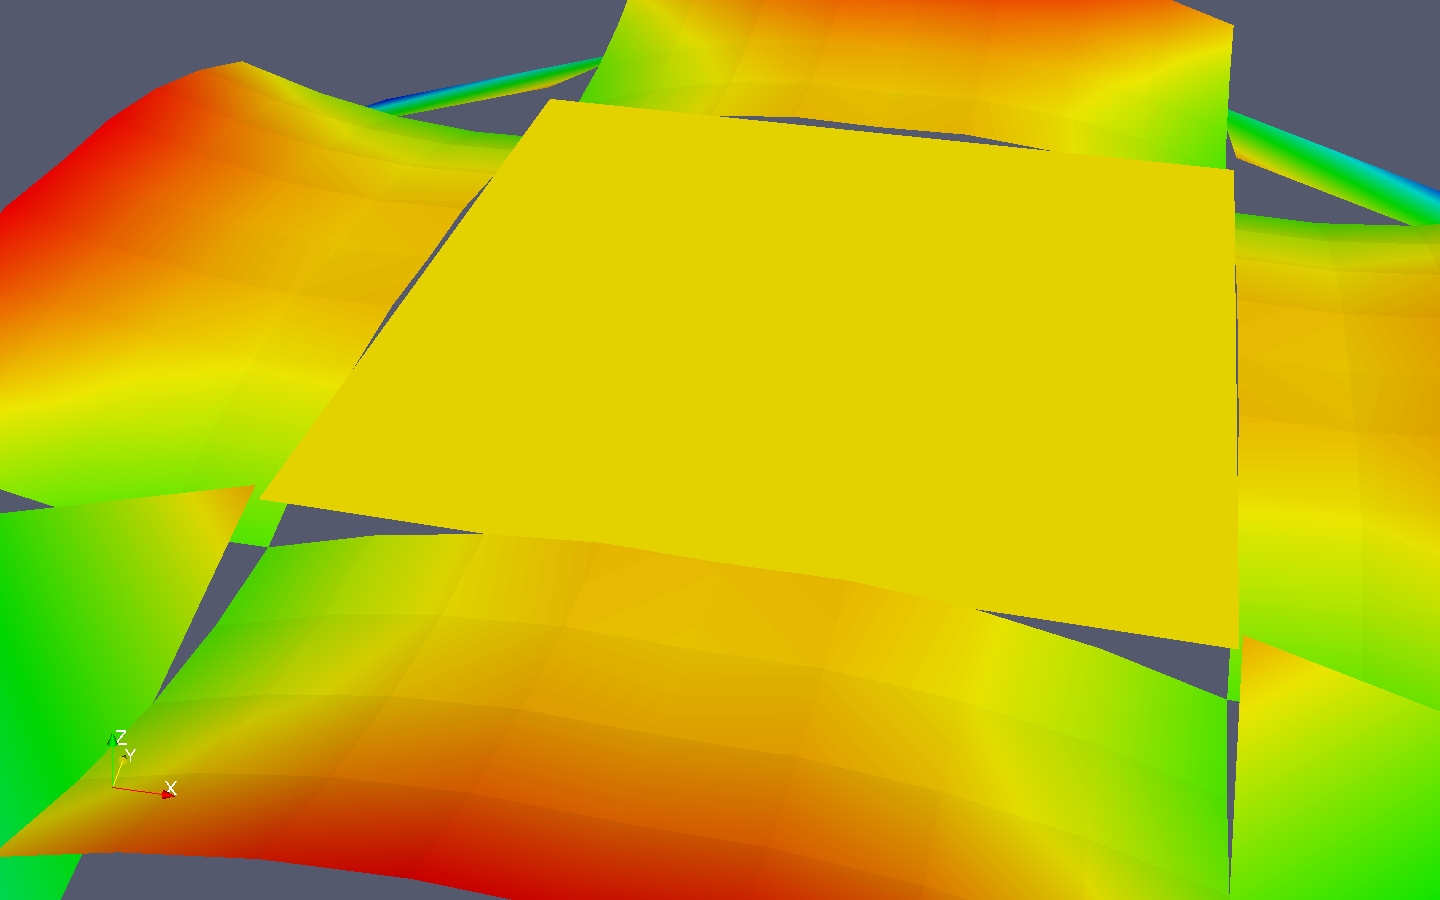
\includegraphics[width=0.9\textwidth]{./EPS/rotbilinear}
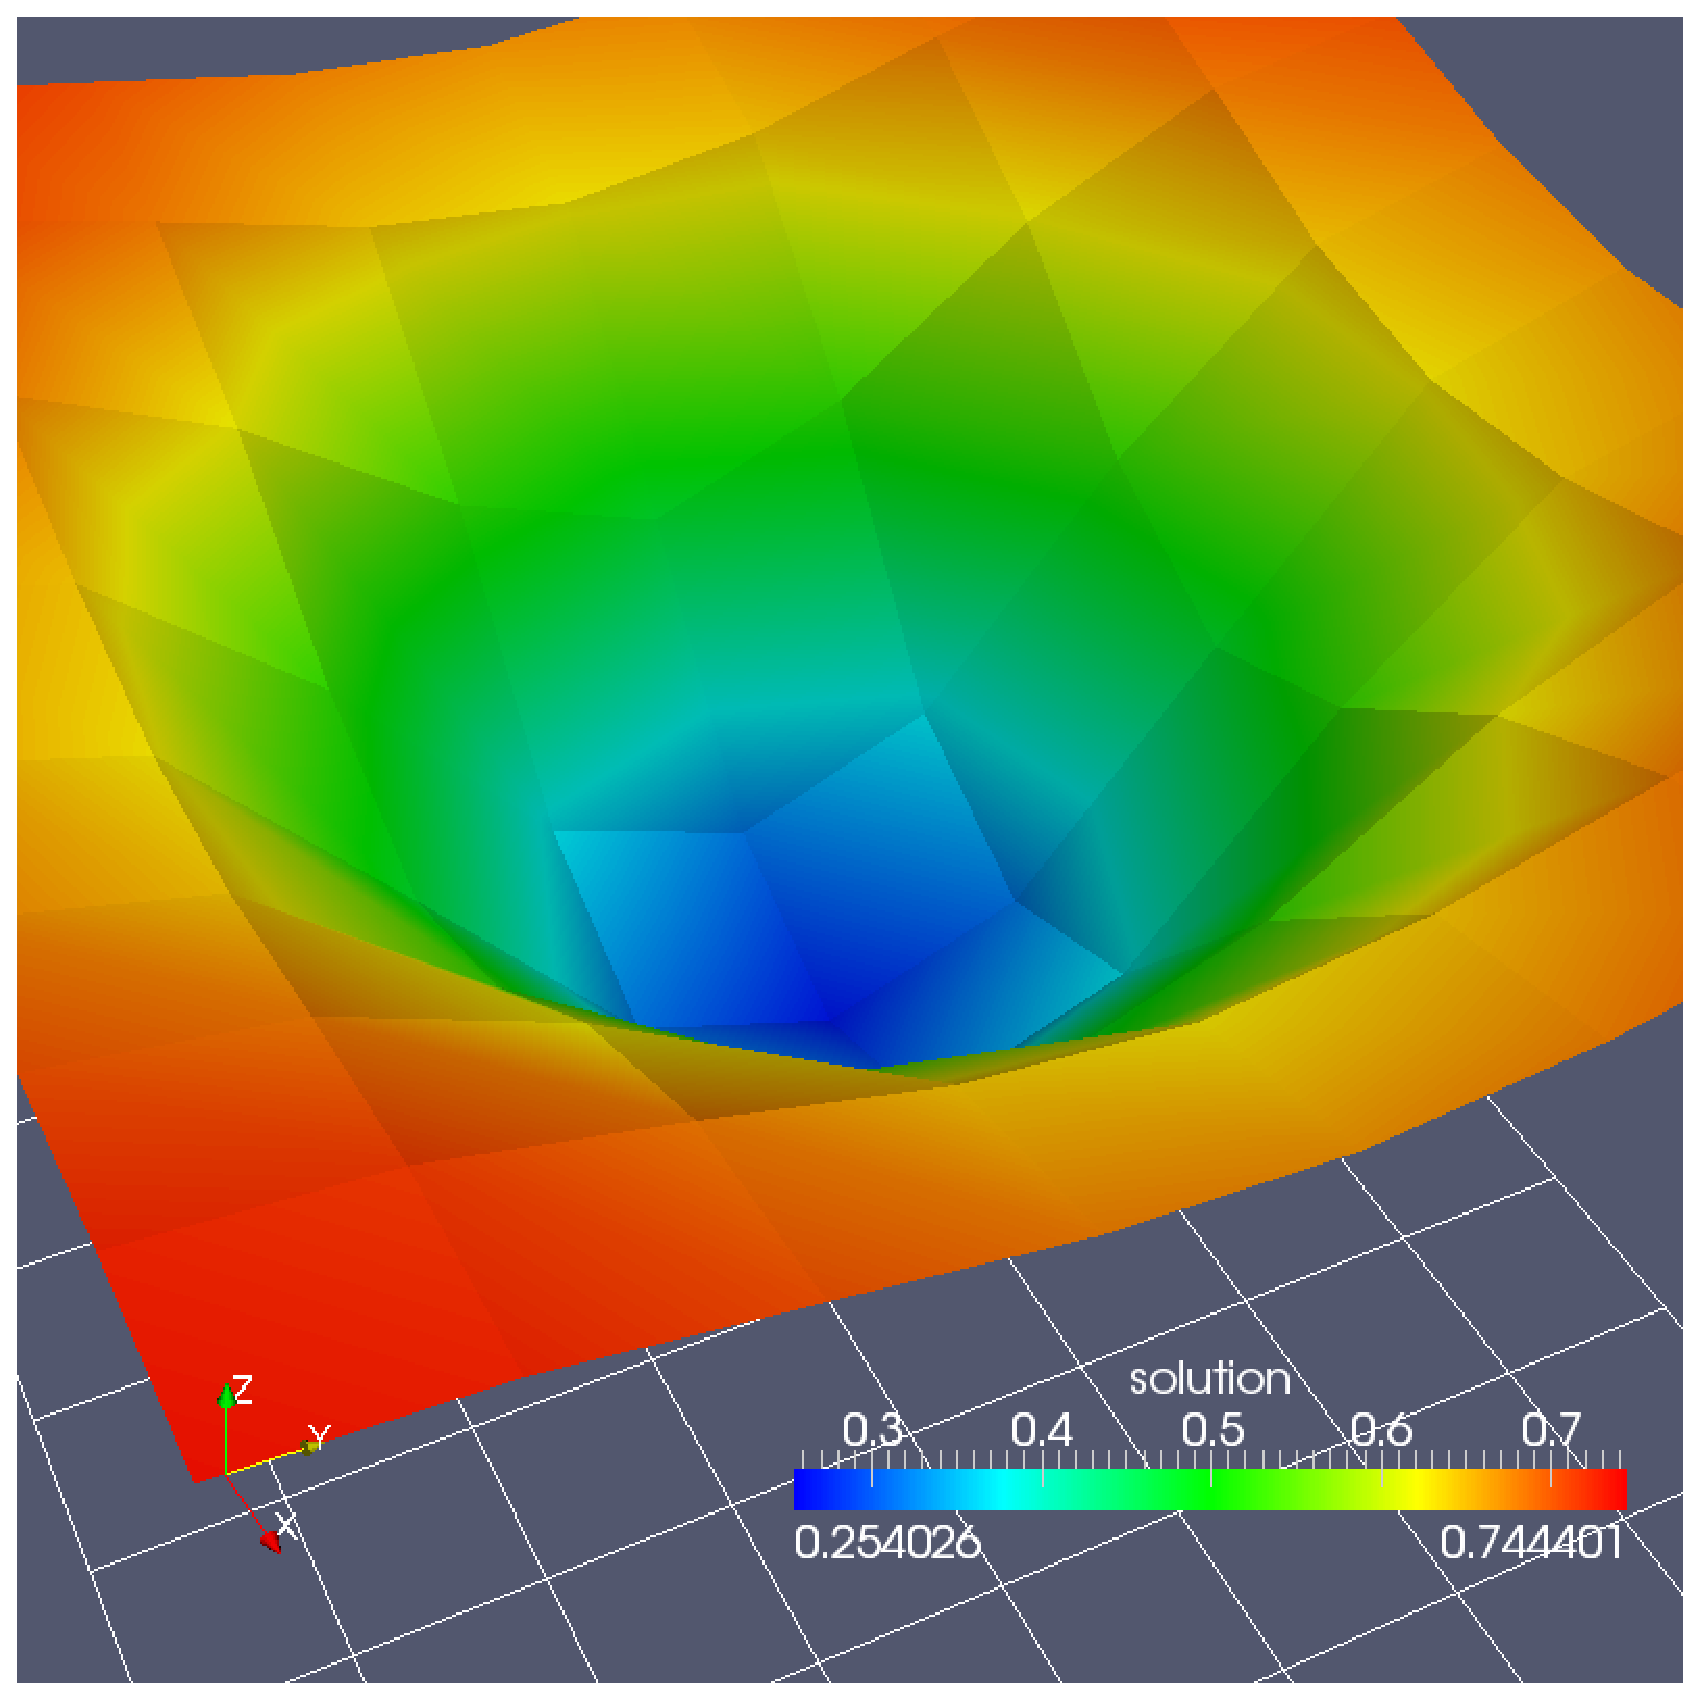
\includegraphics[width=0.32\textwidth]{./EPS/example01a_Q1} $\hspace{1mm}$
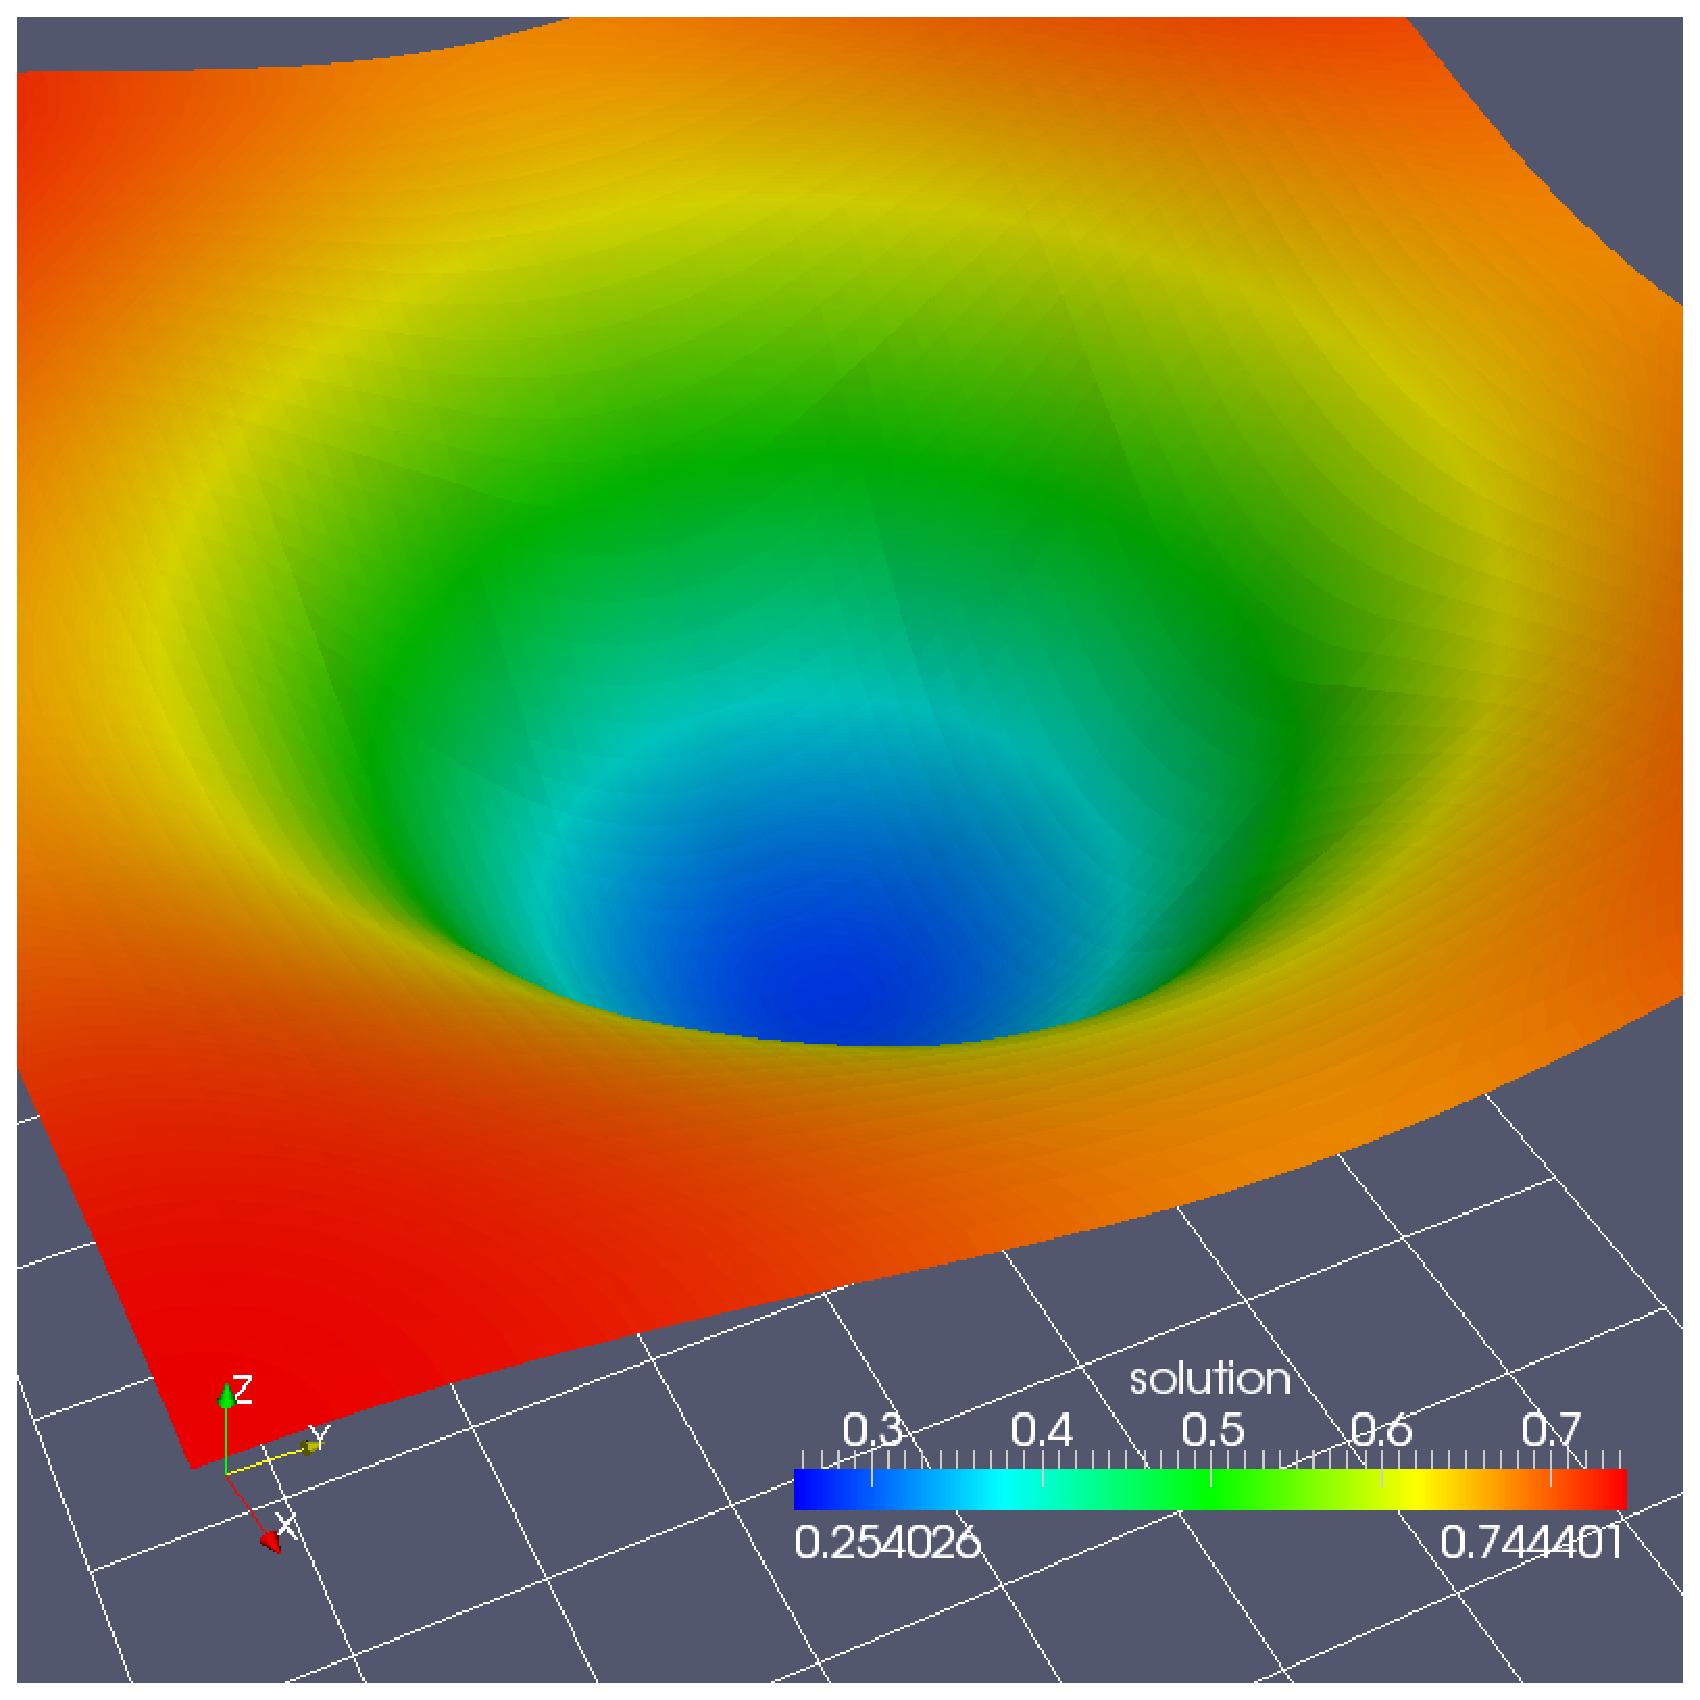
\includegraphics[width=0.32\textwidth]{./EPS/example01a_Q2} $\hspace{1mm}$
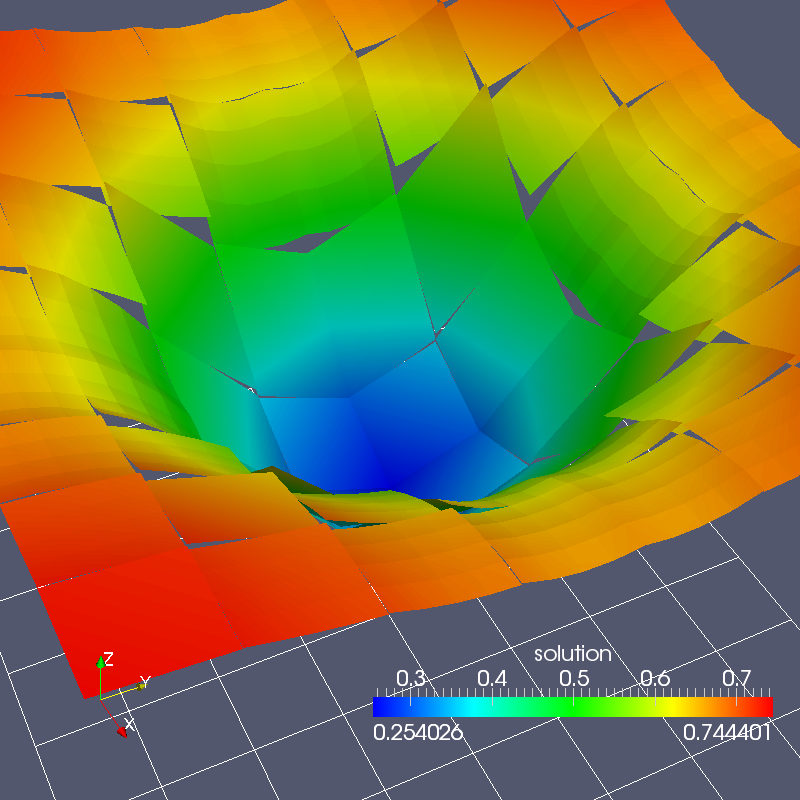
\includegraphics[width=0.32\textwidth]{./EPS/example01a_RT}
  \\
  \vspace{10mm}
  \url{http://www.dune-project.org/}\\
  }
}

% logo nach oben
\mode<presentation>
{
% No navigation symbols and no lower logo
\setbeamertemplate{sidebar right}{}

% logo
\newsavebox{\logobox}
\sbox{\logobox}{%
    \hskip\paperwidth%
    \rlap{%
      % putting the logo should not change the vertical possition
      \vbox to 0pt{%
        \vskip-\paperheight%
        \vskip0.35cm%
        \llap{\insertlogo\hskip0.1cm}%
        % avoid overfull \vbox messages
        \vss%
      }%
    }%
}

\addtobeamertemplate{footline}{}{%
    \usebox{\logobox}%
}
}

% number equations within sections in article mode
%\numberwithin{equation}{section}

% math symbols
\newcommand{\diffd}{\,d}

%%%%%%%%%%%%%%%%%%%%%%%%%%%%%%%%%%%%%%%%%%%%%%%%%%%%%%%%%%%%%%%%%%%%%%%%%%%%%%%%
%%%%%%%%%%%%%%%%%%%%%%%%%%%%%%%%%%%%%%%%%%%%%%%%%%%%%%%%%%%%%%%%%%%%%%%%%%%%%%%%
%
% now comes the individual stuff lecture by lecture
%
%%%%%%%%%%%%%%%%%%%%%%%%%%%%%%%%%%%%%%%%%%%%%%%%%%%%%%%%%%%%%%%%%%%%%%%%%%%%%%%%
%%%%%%%%%%%%%%%%%%%%%%%%%%%%%%%%%%%%%%%%%%%%%%%%%%%%%%%%%%%%%%%%%%%%%%%%%%%%%%%%
\mode<article>
{
\pagestyle{scrheadings}
}

\begin{document}

\mode<presentation>
{
  \begin{frame}
    \titlepage
    % Make sure the cite from the abstract is included in the bibliography, even
    % if the abstract itself is skipped.  Needs to be inside a frame,
    % otherwise presentation mode will ignore it.
    \nocite{Dune2008a,Dune2008b}
  \end{frame}
}
\mode<article>
{
\maketitle
}

\begin{abstract}
This article contains concepts for a general discretization module for
the ``Distributed Numerics Environment'' DUNE \cite{Dune2008a,Dune2008b}. It should enable one
to build up a library of finite element methods in an easy and
extendable way that is closely related to the mathematical formulation
of finite element methods. 
\end{abstract}

\mode<article>
{
\cleardoublepage
}

\mode<presentation>{
\begin{frame}<presentation>
\frametitle{Outline}
\tableofcontents[section,sectionstyle=show/show,subsectionstyle=hide/hide/hide] 
\end{frame}
}

\mode<article>
{
\tableofcontents
}

\mode<article>
{
\cleardoublepage
}

%%%%%%%%%%%%%%%%%%%%%%%%%%%%%%%%%%%%%%%%%%%%%%%%%%%%%%%%%%%%
%%%%%%%%%%%%%%%%%%%%%%%%%%%%%%%%%%%%%%%%%%%%%%%%%%%%%%%%%%%%
%      Sections
%%%%%%%%%%%%%%%%%%%%%%%%%%%%%%%%%%%%%%%%%%%%%%%%%%%%%%%%%%%%
%%%%%%%%%%%%%%%%%%%%%%%%%%%%%%%%%%%%%%%%%%%%%%%%%%%%%%%%%%%%
\mode<all>{%%%%%%%%%%%%%%%%%%%%%%%%%%%%%%%%%%%%%%%%%%%%%%%%%%%%%%%%%%%%
%%%%%%%%%%%%%%%%%%%%%%%%%%%%%%%%%%%%%%%%%%%%%%%%%%%%%%%%%%%%
%%%%%%%%%%%%%%%%%%%%%%%%%%%%%%%%%%%%%%%%%%%%%%%%%%%%%%%%%%%%
\section{Introduction}
%%%%%%%%%%%%%%%%%%%%%%%%%%%%%%%%%%%%%%%%%%%%%%%%%%%%%%%%%%%%
%%%%%%%%%%%%%%%%%%%%%%%%%%%%%%%%%%%%%%%%%%%%%%%%%%%%%%%%%%%%
%%%%%%%%%%%%%%%%%%%%%%%%%%%%%%%%%%%%%%%%%%%%%%%%%%%%%%%%%%%%

\subsection{PDELab Aims and Features}

\begin{frame}
\frametitle<presentation>{DUNE Module Architecture}
Major DUNE modules are:
\begin{center}
\mode<presentation>{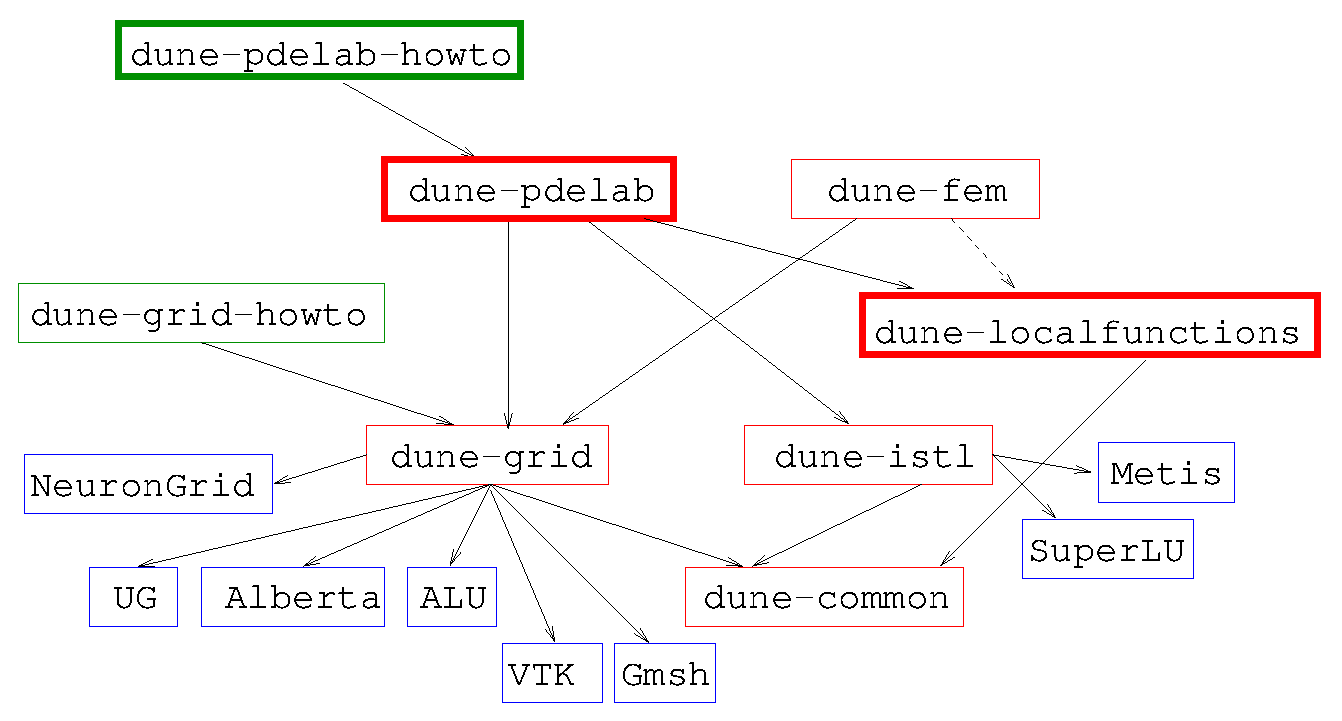
\includegraphics[width=1.0\textwidth]{./EPS/modules}}
\mode<article>{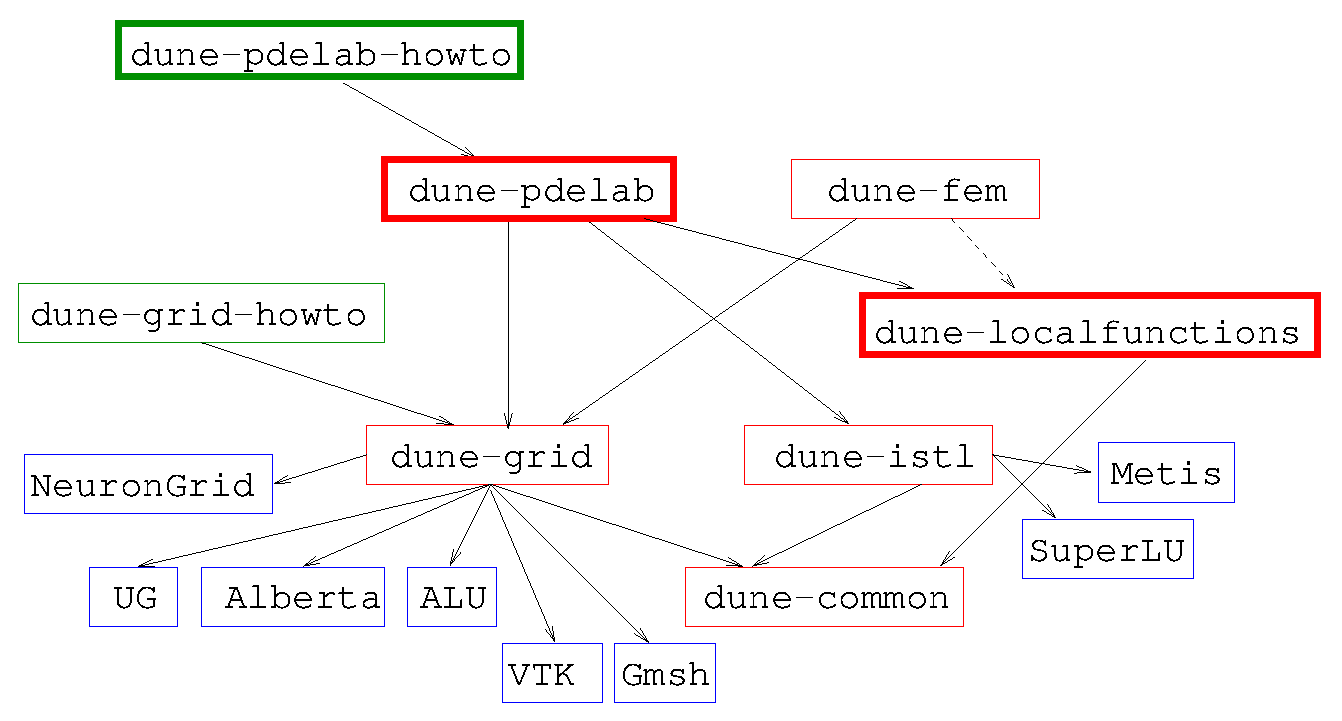
\includegraphics[width=0.7\textwidth]{./EPS/modules}}
\end{center}
\end{frame}

\begin{frame}
\frametitle<presentation>{DUNE PDELab Features}
\begin{itemize}
\item Rapid prototyping: Substantially reduce time to implement
discretizations and solvers for systems of PDEs based on DUNE.
\item Simple things should be simple --- suitable for teaching.
\item Discrete function spaces spaces:
\begin{itemize}
\item Conforming and non-conforming,
\item hp-refinement,
\item general approach to constraints,
\item generic generation of product spaces for systems.
\end{itemize} 
\item Operators based on weighted residual formulation:
\begin{itemize}
\item Linear and nonlinear,
\item stationary and transient,
\item FE and FV schemes requiring at most face-neighbors.
\end{itemize} 
\item Exchangeable linear algebra backend. 
\item User only involved with ``local'' view on (reference) element.
\end{itemize}
\end{frame}

\begin{frame}
\frametitle<presentation>{Coding Effort}
\begin{center}
\small\begin{tabular}{|p{0.5\textwidth}|p{0.3\textwidth}|r|}
\hline
Problem & Scheme & LOC \\
\hline
\hline
$\nabla\cdot\{v u - K\nabla u\}=f$ & $P_k, Q_k$ & 643 \\
 & DG & 1034 \\
\hline
$-\nabla\cdot\{K\nabla u\}=f$ & CCFV & 223 \\
 & RT$_0$ & 289 \\
 & Mimetic & 278 \\
\hline
Two-phase flow in porous media & $p_l, p_c$, CCFV & 700 \\
& $p_l, p_c$, DG & 931 \\  
& CCFV, 2c & 986 \\
\hline
Navier-Stokes & $P_2/P_1$, $Q_2/Q_1$ & 539 \\
           & DG & 1122 \\
\hline
Linear acoustics & DG & 700 \\
\hline
Maxwell in time domain & DG & 857 \\
 & Nedelec & 488 \\
\hline
\end{tabular}
\end{center}
This does \textbf{not} include finite element spaces and problem setup.
\end{frame}

\begin{frame}
\frametitle<presentation>{Required Modules}
To work through the examples the following DUNE modules are required: 
\begin{itemize}
\item \lstinline{dune-common},
\item \lstinline{dune-geometry},
\item \lstinline{dune-grid},
\item \lstinline{dune-istl},
\item \lstinline{dune-localfunctions},
\item \lstinline{dune-pdelab},
\item \lstinline{dune-pdelab-howto},
\end{itemize}

In addition, at least one of the grid managers UG, ALU or Alberta is
required to do the examples on simplex grids. 
\end{frame}



\subsection{How to Read this Manual}

The main idea of this howto is to introduce the concepts by working
through a set of increasingly complex examples. We will start by 
solving stationary elliptic problems first without and then with constrained spaces
(Dirichlet boundary conditions). After some excursion to linear algebra backends and 
working with CAD models instationary problems and systems will be treated.

\cleardoublepage
}
\mode<all>{%%%%%%%%%%%%%%%%%%%%%%%%%%%%%%%%%%%%%%%%%%%%%%%%%%%%%%%%%%%%
%%%%%%%%%%%%%%%%%%%%%%%%%%%%%%%%%%%%%%%%%%%%%%%%%%%%%%%%%%%%
%%%%%%%%%%%%%%%%%%%%%%%%%%%%%%%%%%%%%%%%%%%%%%%%%%%%%%%%%%%%
\section{Solving Stationary Problems}\label{Sec:EllipticProblems}
%%%%%%%%%%%%%%%%%%%%%%%%%%%%%%%%%%%%%%%%%%%%%%%%%%%%%%%%%%%%
%%%%%%%%%%%%%%%%%%%%%%%%%%%%%%%%%%%%%%%%%%%%%%%%%%%%%%%%%%%%
%%%%%%%%%%%%%%%%%%%%%%%%%%%%%%%%%%%%%%%%%%%%%%%%%%%%%%%%%%%%

\begin{frame}
\frametitle<presentation>{Abstraction}
\begin{itemize}
\item Code reuse requires abstraction.
\item Abstractions for function spaces.
\item Abstractions for PDE discretizations.
\end{itemize}
\end{frame}

\subsection{Unconstrained Elliptic Model Problem}

\begin{frame}
\frametitle{Problem and Weak Formulation}
Consider the following model problem:
\begin{subequations} \label{Eq:Example01}
\begin{align*}
-\Delta u + a u &= f &&\text{in $\Omega\subset\mathbb{R}^d$ (open, connected)},\\
\nabla u \cdot n &= 0 &&\text{on $\partial\Omega$}.
\end{align*}
\end{subequations}
\medskip
Weak formulation. Set $U = H^1(\Omega)$.
\begin{equation*}
u\in U \quad : \quad \underbrace{\int_\Omega \nabla u \cdot \nabla v + 
a u v - f v \,dx}_{r(u,v)} = 0 \qquad \forall v\in U.
\end{equation*}
Has unique solution for $a(x)\geq a_0>0$.

We call $r(u,v)$ residual form.

Other boundary conditions are treated later.
\end{frame}

\begin{frame}
\frametitle{Conforming Finite Element Method}
Needs conforming triangulation $E_h^0 = \{e_o,\ldots,e_{N_h^0-1} \}$ of $\Omega$. 

Define the conforming finite element space
\begin{equation*}
U_h^k = \left\{  u\in C^0(\overline{\Omega}) \ : \ u|_{\Omega_e} \in P_{k_e} \forall e\in E_h^0\right\} \subset H^1(\Omega).
\end{equation*}
\begin{itemize}
\item $\Omega_e$: domain of element $e\in E_h^0$.
\item $P_k$: Polynomials of degree $k$.
\item $k_e$: Polynomial degree on element $e$.
\end{itemize}
Discrete problem then reads:
\begin{equation*}
u_h \in U_h^k \quad : \quad r(u_h,v) = 0 \qquad \forall v \in U_h^k.
\end{equation*}
\end{frame}

\begin{frame}
\frametitle{Affine Finite Element Spaces}
Construct functions in $U_h^k$ from local basis on reference elements:
\begin{equation*}
U_h^k\ni u_h(x) = \sum_{e\in E_h^0} \sum_{l=0}^{n(e)-1} (\mathbf{u})_{g(e,l)}
\, \hat{\phi}_{e,l}(\mu_e^{-1}(x)) \, \chi_e(x).
\end{equation*}
\begin{itemize}
\item $n(e)$: Number of basis functions on element $e\in E_h^0$.
\item $\hat\Omega_e$: Reference element of element $e\in E_h^0$.
\item $\mu_e : \hat\Omega_e \to \Omega_e$: Element transformation.
\item $\hat\phi_{e,l} : \hat\Omega_e \to \mathbb{R}$: Local basis function.
\item $\mathcal{I}_{U_h^k} = \{0,\ldots,N_{U_h^k}-1\}$: Global index set.
\item $g : E_h^0 \times \mathbb{N}_0 \to \mathcal{I}_{U_h^k}$: Local to global index map.
\item $\mathbf{u} \in \mathbf{U} = \mathbb{R}^{\mathcal{I}_{U_h^k}}$: Global vector of degrees of freedom.
\item $\chi_e$: Characteristic function of element $e$.
\end{itemize}
Note: We might have a different set of basis functions on each element.
\end{frame}

\begin{frame}
\frametitle{Global Basis; Finite Element Isomorphism}
For $j\in \mathcal{I}_{U_h^k}$ set $L(j) = \{ (e,l) \, : \, g(e,l) = j\}$ (all local degrees 
of freedom associated with global degree of freedom $j$.

Global basis:
\begin{equation*}
\Phi_{U_h^k} = \left\{ \phi_j(x) = \sum_{(e,l)\in L(j)} \hat{\phi}_{e,l}(\mu_e^{-1}(x)) \, \chi_e(x) 
\, : \, j \in \mathcal{I}_{U_h^k} \right\}.
\end{equation*}

Finite Element Isomorphism:
\begin{align*}
\text{FE}_{\Phi_{U_h^k}} : \mathbf{U} &\to U_h^k, &
\text{FE}_{\Phi_{U_h^k}}(\mathbf{u}) &= \sum_{j\in \mathcal{I}_{U_h^k}} (\mathbf{u})_j \phi_j.
\end{align*}
\end{frame}

\begin{frame}
\frametitle{Algebraic Problem}
Using the basis the discrete problem can be written equivalently as a (in general nonlinear) algebraic problem:
\begin{align*}
&&& u_h \in U_h^k \quad : \quad r(u_h,v) = 0 && \forall v \in U_h^k,\\
&\Leftrightarrow && \mathbf{u}\in\mathbf{U} \quad : \quad
r\left(\text{FE}_{\Phi_{U_h^k}}(\mathbf{u}),\phi_i\right) = 0 &&
i\in\mathcal{I}_{U_h^k}, \\
&\Leftrightarrow && \mathbf{u}\in\mathbf{U} \quad : \quad
\mathcal{R}(\mathbf{u}) = \mathbf{0}.
\end{align*}
where
\begin{align*}
\mathcal{R} &: \mathbf{U} \to \mathbf{U}, &
\left(\mathcal{R}(\mathbf{u}) \right)_i :=  r\left(\text{FE}_{\Phi_{U_h^k}}(\mathbf{u}),\phi_i\right) .
\end{align*}

For linear PDEs $\mathcal{R}$ is affine linear: $\mathcal{R}(\mathbf{u}) = \mathbf{A} \mathbf{u} - \mathbf{b}$.
\end{frame}

\begin{frame}
\frametitle{Residual Assembly}
\begin{equation*}
\begin{split}
&(\mathcal{R}(\mathbf{u}) )_i  = r\left(\text{FE}(\mathbf{u}),\phi_i\right)
= \sum_{e\in E_h^0} \int_{\Omega_e} \nabla \text{FE}(\mathbf{u}) \cdot \nabla\phi_i 
+ a \, \text{FE}_{\Phi_{U_h^k}}(\mathbf{u}) \phi_i - f \phi_i \,dx\\
&= \sum_{e\in E_h^0} \int_{\Omega_e} 
\left[ \sum_{l=0}^{n(e)-1} (\mathbf{u})_{g(e,l)} \nabla_x \hat\phi_{e,l}(\mu_e^{-1}(x))\right]
\cdot \nabla_x \underbrace{\hat\phi_{e,m}}_{g(e,m)=i}(\mu_e^{-1}(x))\\
& + a \, \left[ \sum_{l=0}^{n(e)-1} (\mathbf{u})_{g(e,l)} \hat\phi_{e,l}(\mu_e^{-1}(x)) \right] \hat\phi_{e,m}(\mu_e^{-1}(x))
- f \hat\phi_{e,m}(\mu_e^{-1}(x)) \, dx\\
&= \sum_{e\in E_h^0} \int_{\hat\Omega_e} 
\Biggl\{\left[ \sum_{l=0}^{n(e)-1} (\mathbf{u})_{g(e,l)} (\nabla \mu_e(\hat{x}))^{-T}\nabla_{\hat{x}} \hat\phi_{e,l}(\hat{x})\right]
\cdot (\nabla \mu_e(\hat{x}))^{-T} \nabla_{\hat{x}} \hat\phi_{e,m}(\hat{x})\\
& + a \, \left[ \sum_{l=0}^{n(e)-1} (\mathbf{u})_{g(e,l)} \hat\phi_{e,l}(\hat{x}) \right] \hat\phi_{e,m}(\hat{x})
- f \hat\phi_{e,m}(\hat{x}) \Biggr\} \text{det} \nabla\mu_e(\hat{x}) \, d\hat{x} .
\end{split}
\end{equation*}
\end{frame}

\begin{frame}
\frametitle{Local Operator}
Define restriction to local degrees of freedom
\begin{align*}
\mathbf{U}_e &= \mathbb{R}^{n(e)}, &
\mathbf{R}_e &: \mathbf{U} \to \mathbf{U}_e, &
\left(\mathbf{U}_e(\mathbf{u})\right)_l &= (\mathbf{u})_{g(e,l)} \quad 0\leq l < n(e).
\end{align*}
Define \textit{local operator} $\bm{\alpha}^{\text{vol}}_{h,e} : \mathbf{U}_e \to \mathbf{U}_e$ (user part):
\begin{equation*}
\begin{split}
&\bigl(\bm{\alpha}^{\text{vol}}_{h,e}({\color{cyan}\mathbf{u}})\bigr)_m  = \\
&\sum_{e\in E_h^0} \int_{\hat\Omega_e} 
\Biggl\{\left[ \sum_{l=0}^{n(e)-1} ({\color{cyan}\mathbf{u}})_{l} {\color{purple}
(\nabla \mu_e(\hat{x}))^{-T}} {\color{blue}\nabla_{\hat{x}} \hat\phi_{e,l}(\hat{x})} \right]
\cdot {\color{purple}(\nabla \mu_e(\hat{x}))^{-T}} {\color{blue}\nabla_{\hat{x}} \hat\phi_{e,m}(\hat{x})}\\
& + {\color{olive} a} \, \left[ \sum_{l=0}^{n(e)-1} ({\color{cyan}\mathbf{u}})_{l}
 {\color{blue}\hat\phi_{e,l}(\hat{x})} \right] {\color{blue}\hat\phi_{e,m}(\hat{x})}
- {\color{olive} f} {\color{blue}\hat\phi_{e,m}(\hat{x})} \Biggr\} {\color{purple}\text{det} \nabla\mu_e(\hat{x})} \, d\hat{x} .
\end{split}
\end{equation*}
Residual assembly is written generically:
\begin{equation*}
\mathcal{R}(\mathbf{u}) = \sum_{e\in E_h^0} \mathbf{R}_e^T \bm{\alpha}^{\text{vol}}_{h,e} (\mathbf{R}_e \mathbf{u})
\end{equation*}
\end{frame}


\begin{frame}
\frametitle{Solving the Algebraic System}
Use damped Newton method.

Given $\mathbf{u}^0\in\mathbf{U}$. Compute $\mathbf{r}^0 = \mathcal{R}(\mathbf{u}^0)$. Set $k=0$.

Iterate until convergence:
\begin{enumerate}
\item Assemble Jacobian System $\mathbf{A}^k = \nabla\mathcal{R}(\mathbf{u}^k)$.
\item Solve $\mathbf{A}^k \mathbf{z}^k = \mathbf{r}^k$ with some linear solver.
\item Update $\mathbf{u}^{k+1} = \mathbf{u}^{k} - \sigma^k \mathbf{z}^{k+1}$. $\sigma\in(0,1]$.
\item Compute new residual $\mathbf{r}^{k+1} = \mathcal{R}(\mathbf{u}^{k+1})$.
\item Set $k = k +1$.
\end{enumerate}

We need methods to compute $\mathcal{R}(\mathbf{u})$ and $\nabla\mathcal{R}(\mathbf{u})$.
\end{frame}

\begin{frame}
\frametitle{Jacobian}
The Jacobian matrix is defined as
\begin{equation*}
(\mathbf{A}^k)_{i,j} = (\nabla\mathcal{R}(\mathbf{u}^k))_{i,j} 
= \frac{\partial (\mathcal{R})_i}{\partial (\mathbf{u})_j}(\mathbf{u}^k)
= \sum_{e\in E_h^0} \frac{\partial (\bm{\alpha}_{h,e}^{\text{vol}})_m }{\partial (\mathbf{u})_l } (\mathbf{R}_e \mathbf{u}),
\end{equation*}
where $g(e,m)=l, g(e,l)=j$.

Again, the Jacobian can be computed from local contributions:
\begin{equation*}
\mathbf{A}^k = \sum_{e\in E_h^0} \mathbf{R}_e^T \nabla\bm{\alpha}_{h,e}^{\text{vol}}(\mathbf{R}_e \mathbf{u}) \, \mathbf{R}_e.
\end{equation*}

The local Jacobians can be
\begin{itemize}
\item programmed explicitly by the user, or
\item derived generically through numerical differentiation. This requires only coding
of the local residual contributions $\bm{\alpha}_{h,e}^{\text{vol}}$.
\end{itemize}
\end{frame}


\begin{frame}
\frametitle{The Linear Case}
is a special case of the nonlinear case \ldots
\begin{enumerate}
\item Given $\mathbf{u}^0\in\mathbf{U}$.
\item Compute $\mathbf{r} = \mathcal{R}(\mathbf{u}^0)$.
\item Assemble Jacobian System $\mathbf{A} = \nabla\mathcal{R}(\mathbf{u}^0)$.
\item Solve $\mathbf{A} \mathbf{z} = \mathbf{r}$ with some linear solver.
\item Update $\mathbf{u} = \mathbf{u}^{0} - \mathbf{z}$.
\end{enumerate}
\end{frame}

\subsection{Example 1}

\begin{frame}
\frametitle{Example 1 Overview}
The first example implements model problem \eqref{Eq:Example01}.

It consists of the following files:
\begin{itemize}
\item \lstinline{example01.cc} -- the file to be compiled. 
\item \lstinline{example01_main.hh} -- main function. Instantiates a grid and runs the variants.
\item \lstinline{example01a_Q1.hh} -- solve model problem \eqref{Eq:Example01} with $Q_1$ elements.
\item \lstinline{example01a_Q2.hh} -- same with $Q_2$ elements.
\item \lstinline{example01a_RT.hh} -- same with nonconforming rotated bilinear (``Rannacher-Turek'' element).
\item \lstinline{example01a_operator.hh} -- local operator implementing $\bm{\alpha}_{h,e}^{\text{vol}}$.
\item \lstinline{example01b_Q2.hh} -- solve nonlinear variant of the model problem \eqref{Eq:Example01} with $Q_2$ elements.
\item \lstinline{example01b_operator.hh} -- the local operator for the nonlinear variant.
\end{itemize}
\end{frame}

\begin{frame}<presentation>[fragile,allowframebreaks,allowdisplaybreaks]
\frametitle<presentation>{Function \lstinline{main}}
\framesubtitle<presentation>{File \texttt{examples/example01\_main.hh}}
\lstinputlisting[basicstyle=\ttfamily\tiny,numbers=left, 
numberstyle=\tiny, numbersep=2pt]{../../examples/example01_main.hh}
\end{frame}
\mode<article>{
For completeness we show the main function that just instantiates a \lstinline{YaspGrid} object
and calls the variants.

Main functions will not be shown in later examples.

\begin{Lst}[File examples/example01\_main.hh] \mbox
\nopagebreak
\lstinputlisting[basicstyle=\ttfamily\scriptsize,numbers=left, 
numberstyle=\tiny, numbersep=2pt]{../../examples/example01_main.hh}
\end{Lst}}


\begin{frame}
\frametitle{Driver for Solving Stationary Linear Problems}
\framesubtitle{About \lstinline{example01a_Q1.hh}}
\begin{enumerate}
\item Define useful constants/types like dimension or basic numeric type.
\item Make \textit{grid function space} which corresponds here to $U_h^k$. It requires
\begin{itemize}
\item a \textit{finite element map} defining a local basis on each element.
\item a method to set up \textit{constraints} on the function space (empty here).
\item a suitable vector backend.
\end{itemize}
\item Make \textit{grid operator space} computing $\mathcal{R}(\mathbf{u})$, $\nabla\mathcal{R}(\mathbf{u})$. It requires
\begin{itemize}
\item a local operator which provides $\bm{\alpha}_{h,e}^{\text{vol}}$.
\item trial and test grid function spaces, possibly with constraints.
\item a suitable matrix backend.
\end{itemize}
\item Select a linear solver backend (see vector/matrix backend).
\item Solve the linear problem given with the selected solver backend.
\begin{itemize}
\item \textit{Vector container} is used to store degrees of freedom $\mathbf{u}\in\mathbf{U}$.
\end{itemize}
\item Output graphics files to visualize solution with ParaView.
\begin{itemize}
\item \textit{Discrete grid function} implements finite element isomorphism.
\end{itemize}
\end{enumerate}
\end{frame}


\begin{frame}<presentation>[fragile,allowframebreaks,allowdisplaybreaks]
\frametitle<presentation>{Unconstrained Elliptic Problem with $Q_1$}
\framesubtitle<presentation>{File \texttt{examples/example01a\_Q1.hh}}
\lstinputlisting[basicstyle=\ttfamily\tiny,numbers=left, 
numberstyle=\tiny, numbersep=2pt]{../../examples/example01a_Q1.hh}
\end{frame}
\mode<article>{
\begin{Lst}[File examples/example01a\_Q1.hh] \mbox
\nopagebreak
\lstinputlisting[basicstyle=\ttfamily\scriptsize,numbers=left, 
numberstyle=\tiny, numbersep=2pt]{../../examples/example01a_Q1.hh}
\end{Lst}}


\begin{frame}
\frametitle{Local Operator}
\begin{itemize}
\item The local operator implements $\bm{\alpha}_{h,e}^{\text{vol}}$ (and more).
\item Class template \lstinline{GridOperatorSpace} builds on a local operator and
provides $\mathcal{R}(\mathbf{u})$, $\nabla\mathcal{R}(\mathbf{u})$ \textit{generically}.
\item Works for many different discretizations (see below).
\item Works as well for systems of PDEs (see below).
\end{itemize}
\end{frame}

\begin{frame}
\frametitle{Local Operator Implementation}
\framesubtitle{About \lstinline{example01a_operator.hh}}
A local operator is a class providing the following:
\begin{itemize}
\item Flags controlling the sparsity pattern assembly.
\item Method \lstinline{pattern_volume} assembling sparsity pattern (default provided).
\item Flags controlling which terms to assemble.
\item Method \lstinline{alpha_volume} computing $\bm{\alpha}_{h,e}^{\text{vol}}(\mathbf{u})$.
\item Method \lstinline{jacobian_volume} computing $\nabla\bm{\alpha}_{h,e}^{\text{vol}}(\mathbf{u})$. 
This method can be provided generically through numerical differentiation.
\item Method \lstinline{jacobian_apply_volume} computing $\nabla\bm{\alpha}_{h,e}^{\text{vol}}(\mathbf{u})\mathbf{u}$. 
This method can be provided generically through numerical differentiation.
\item Possibly more methods (to be introduced later):
\begin{itemize}
\item \lstinline{alpha_boundary}, \lstinline{alpha_skeleton} -- boundary/interior face integrals.
\item \lstinline{lambda_volume}, \lstinline{lambda_boundary} -- parts of the residual depending on the test function only (optional).
\end{itemize}
\end{itemize}
\end{frame}

\begin{frame}[fragile]
\frametitle{\lstinline{alpha_volume} Method}
The method \lstinline{alpha_volume} has the following signature: 
\begin{lstlisting}[basicstyle=\ttfamily\scriptsize]
template<typename EG, typename LFSU, typename X, 
         typename LFSV, typename R>
void alpha_volume (const EG& eg, const LFSU& lfsu, const X& x, 
                   const LFSV& lfsv, R& r) const;
\end{lstlisting}
Where the arguments are:
\begin{itemize}
\item \lstinline{eg} -- a codim 0 entity $e\in E_h^0$.
\item \lstinline{lfsu} -- local basis $\hat\phi_{e,l}$ for trial space.
\item \lstinline{x} -- local coefficients $(\mathbf{u})_l$.
\item \lstinline{lfsv} -- local basis $\hat\psi_{e,l}$ for the test space 
\item \lstinline{r} -- local contribution to residual (the result).
\end{itemize}
\end{frame}


\begin{frame}<presentation>[fragile,allowframebreaks,allowdisplaybreaks]
\frametitle<presentation>{Local Operator for Unconstrained Elliptic Problem}
\framesubtitle<presentation>{File \texttt{examples/example01a\_operator.hh}}
\lstinputlisting[basicstyle=\ttfamily\tiny,numbers=left, 
numberstyle=\tiny, numbersep=2pt]{../../examples/example01a_operator.hh}
\end{frame}
\mode<article>{
\begin{Lst}[File examples/example01a\_operator.hh] \mbox
\nopagebreak
\lstinputlisting[basicstyle=\ttfamily\scriptsize,numbers=left, 
numberstyle=\tiny, numbersep=2pt]{../../examples/example01a_operator.hh}
\end{Lst}}

\begin{frame}<presentation>
\frametitle{Visualization of Example 1 Results}
Left figure shows the results for $Q_1$ elements.

But we can do easily other elements as well \ldots

\begin{center}
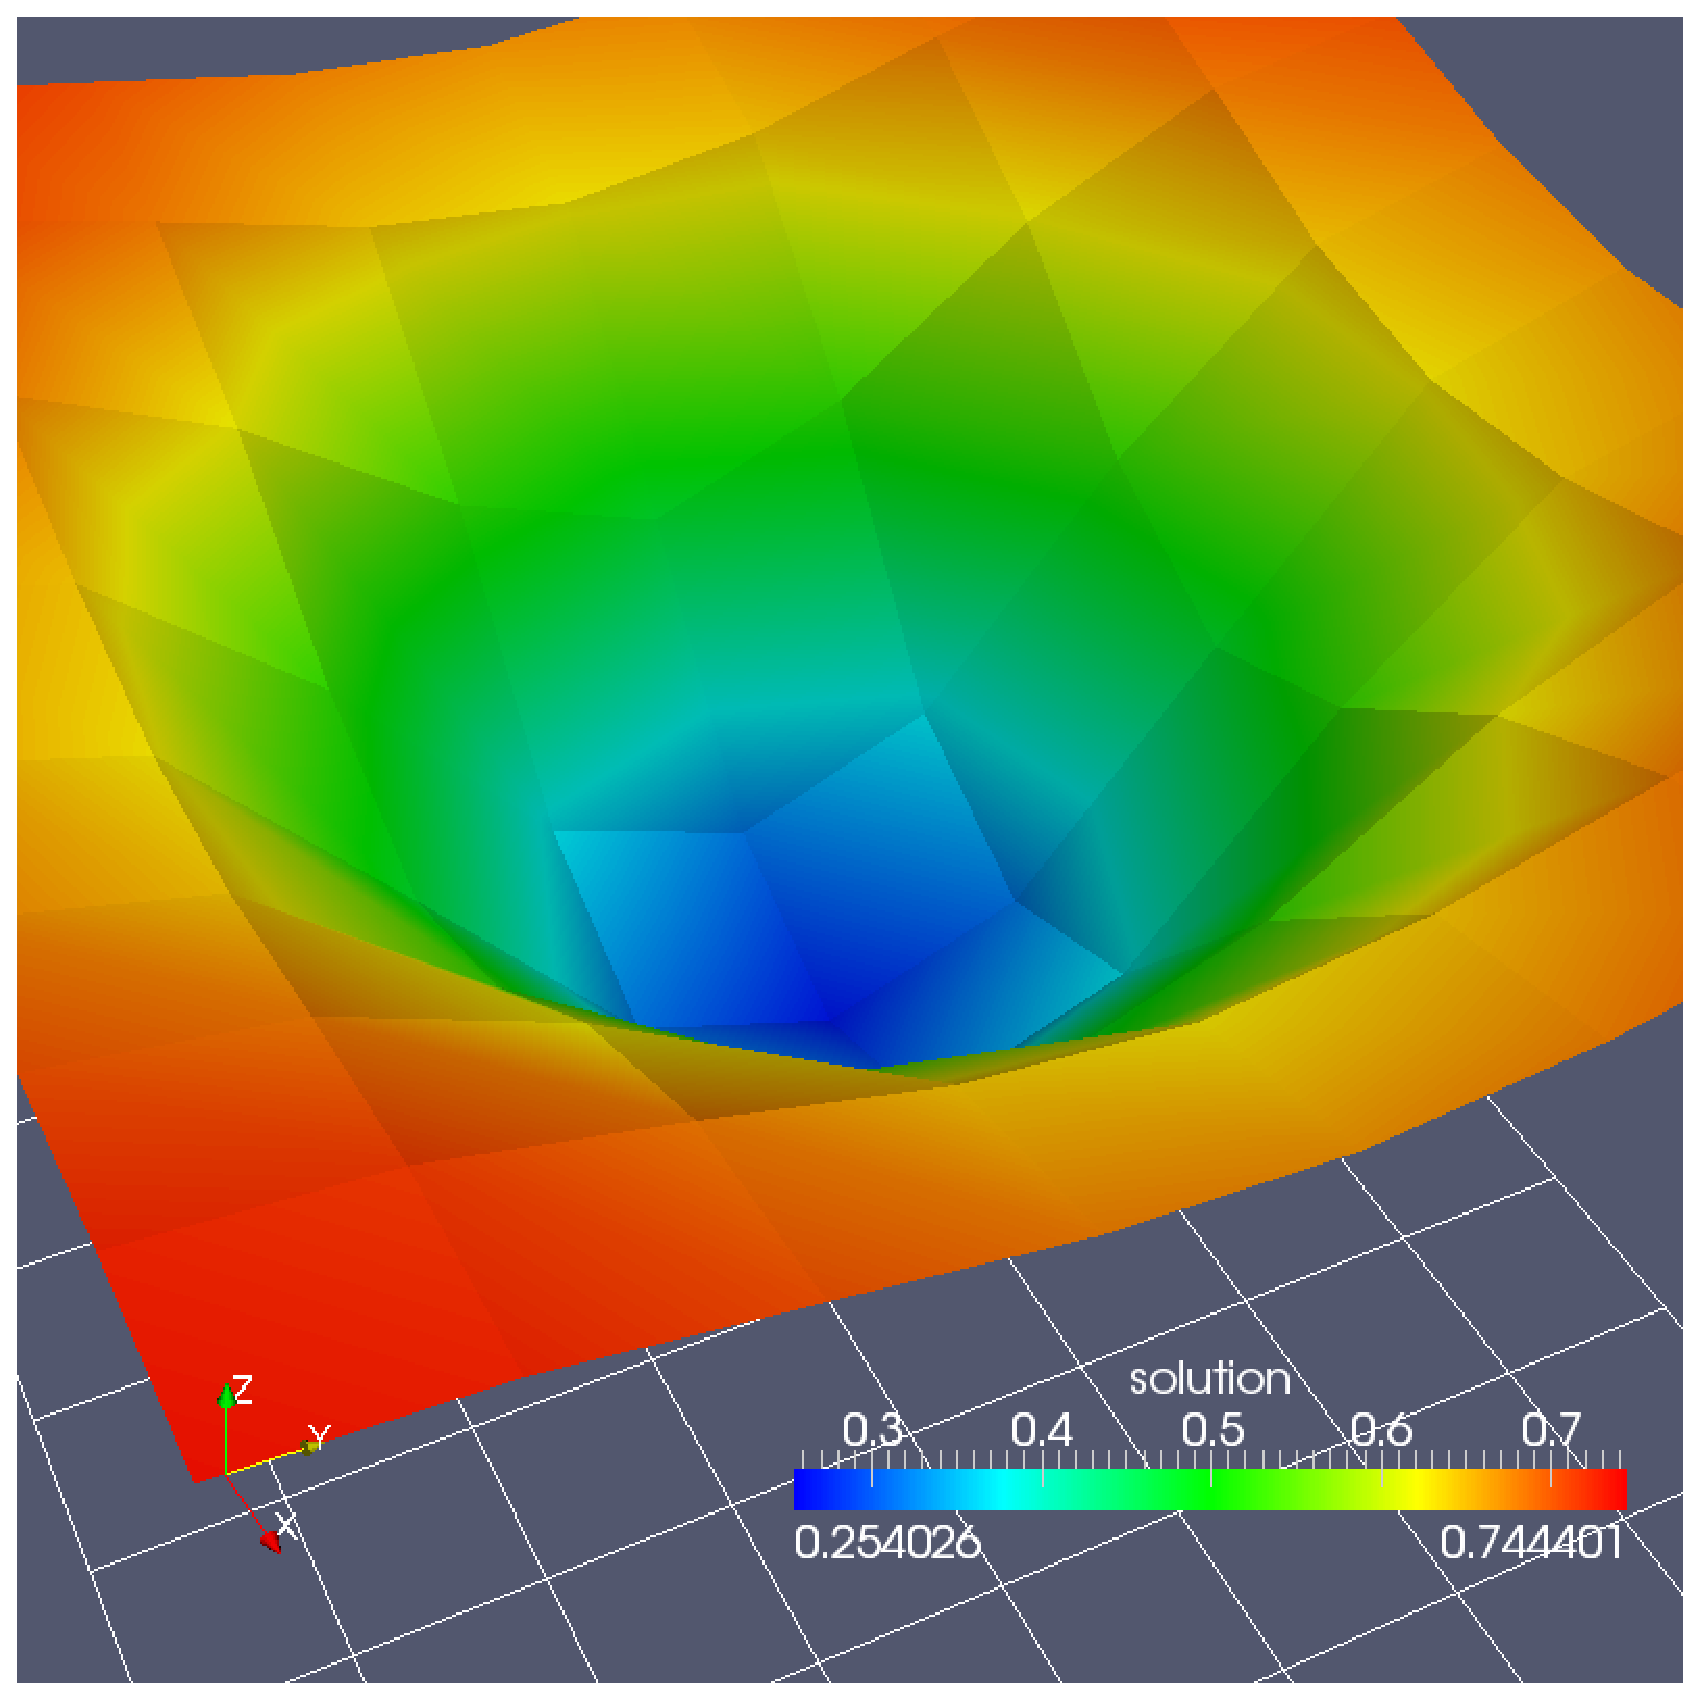
\includegraphics[width=0.32\textwidth]{./EPS/example01a_Q1} $\hspace{1mm}$
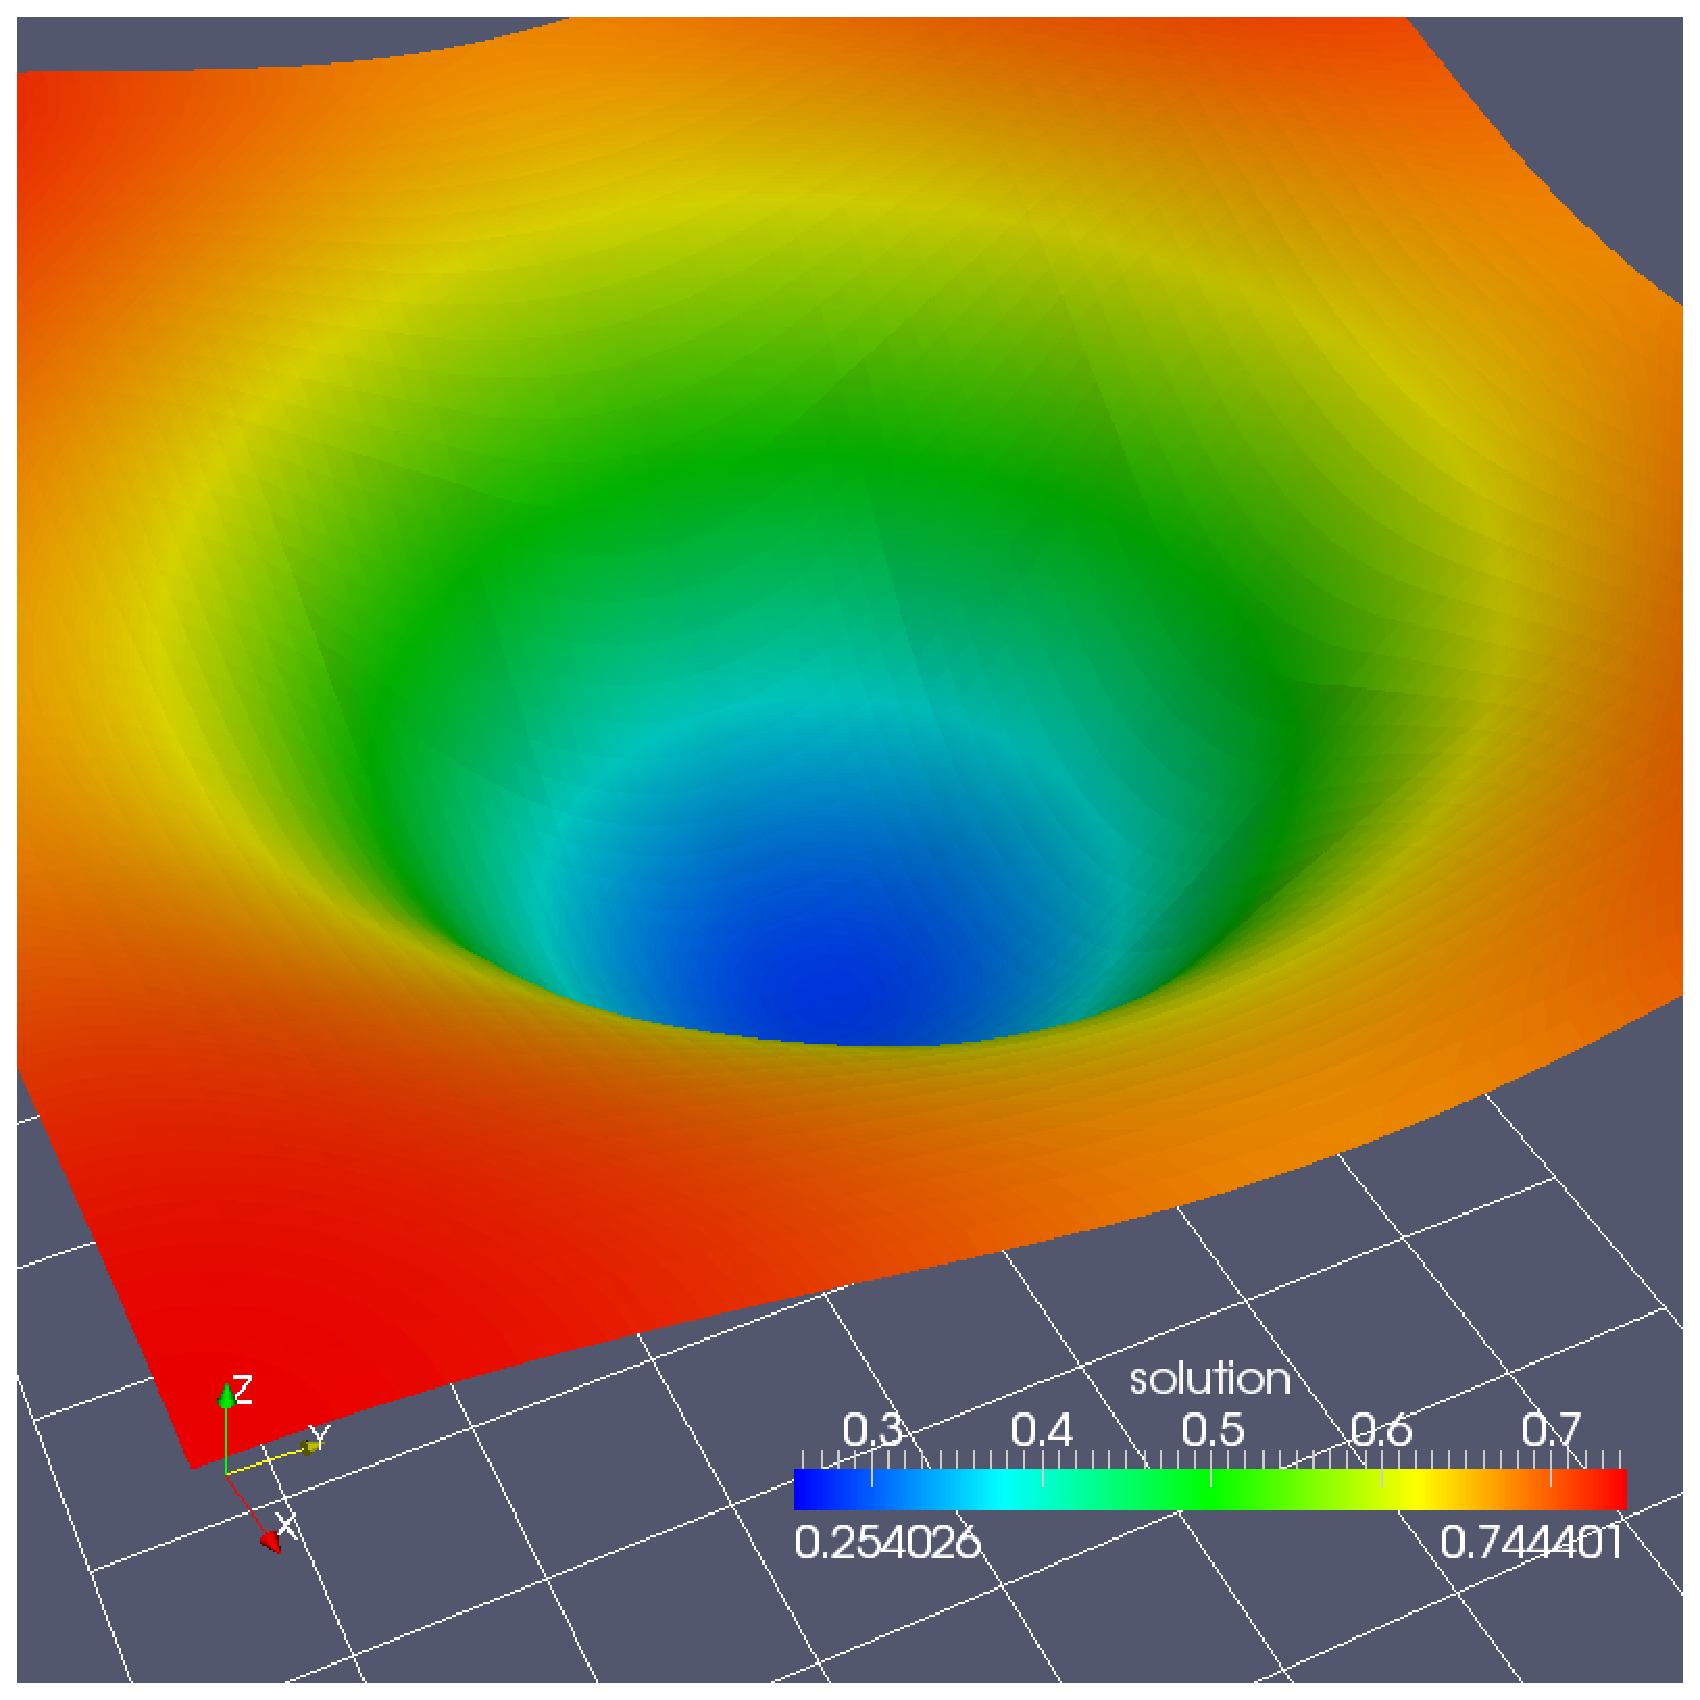
\includegraphics[width=0.32\textwidth]{./EPS/example01a_Q2} $\hspace{1mm}$
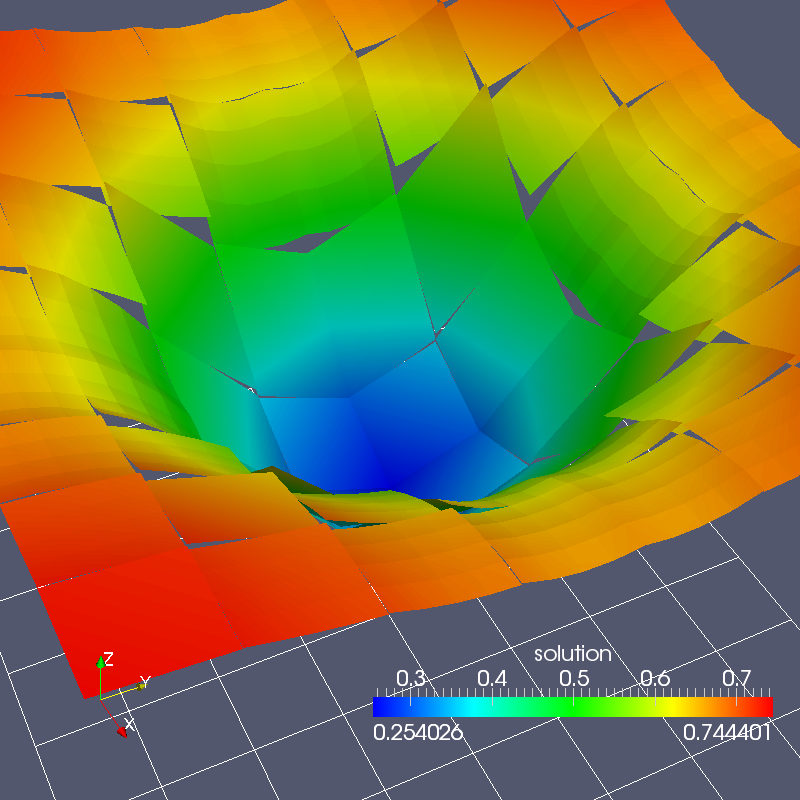
\includegraphics[width=0.32\textwidth]{./EPS/example01a_RT}

$Q_1$ \hspace{30mm} $Q_2$ \hspace{30mm} $RT$
\end{center}

\mode<presentation>{
More on that in the excercises!
}
\end{frame}

\mode<article>{
Figure \ref{fig:Example01aResults} shows visualizations of the results computed
with \lstinline{example01}.
\begin{figure}
\begin{center}
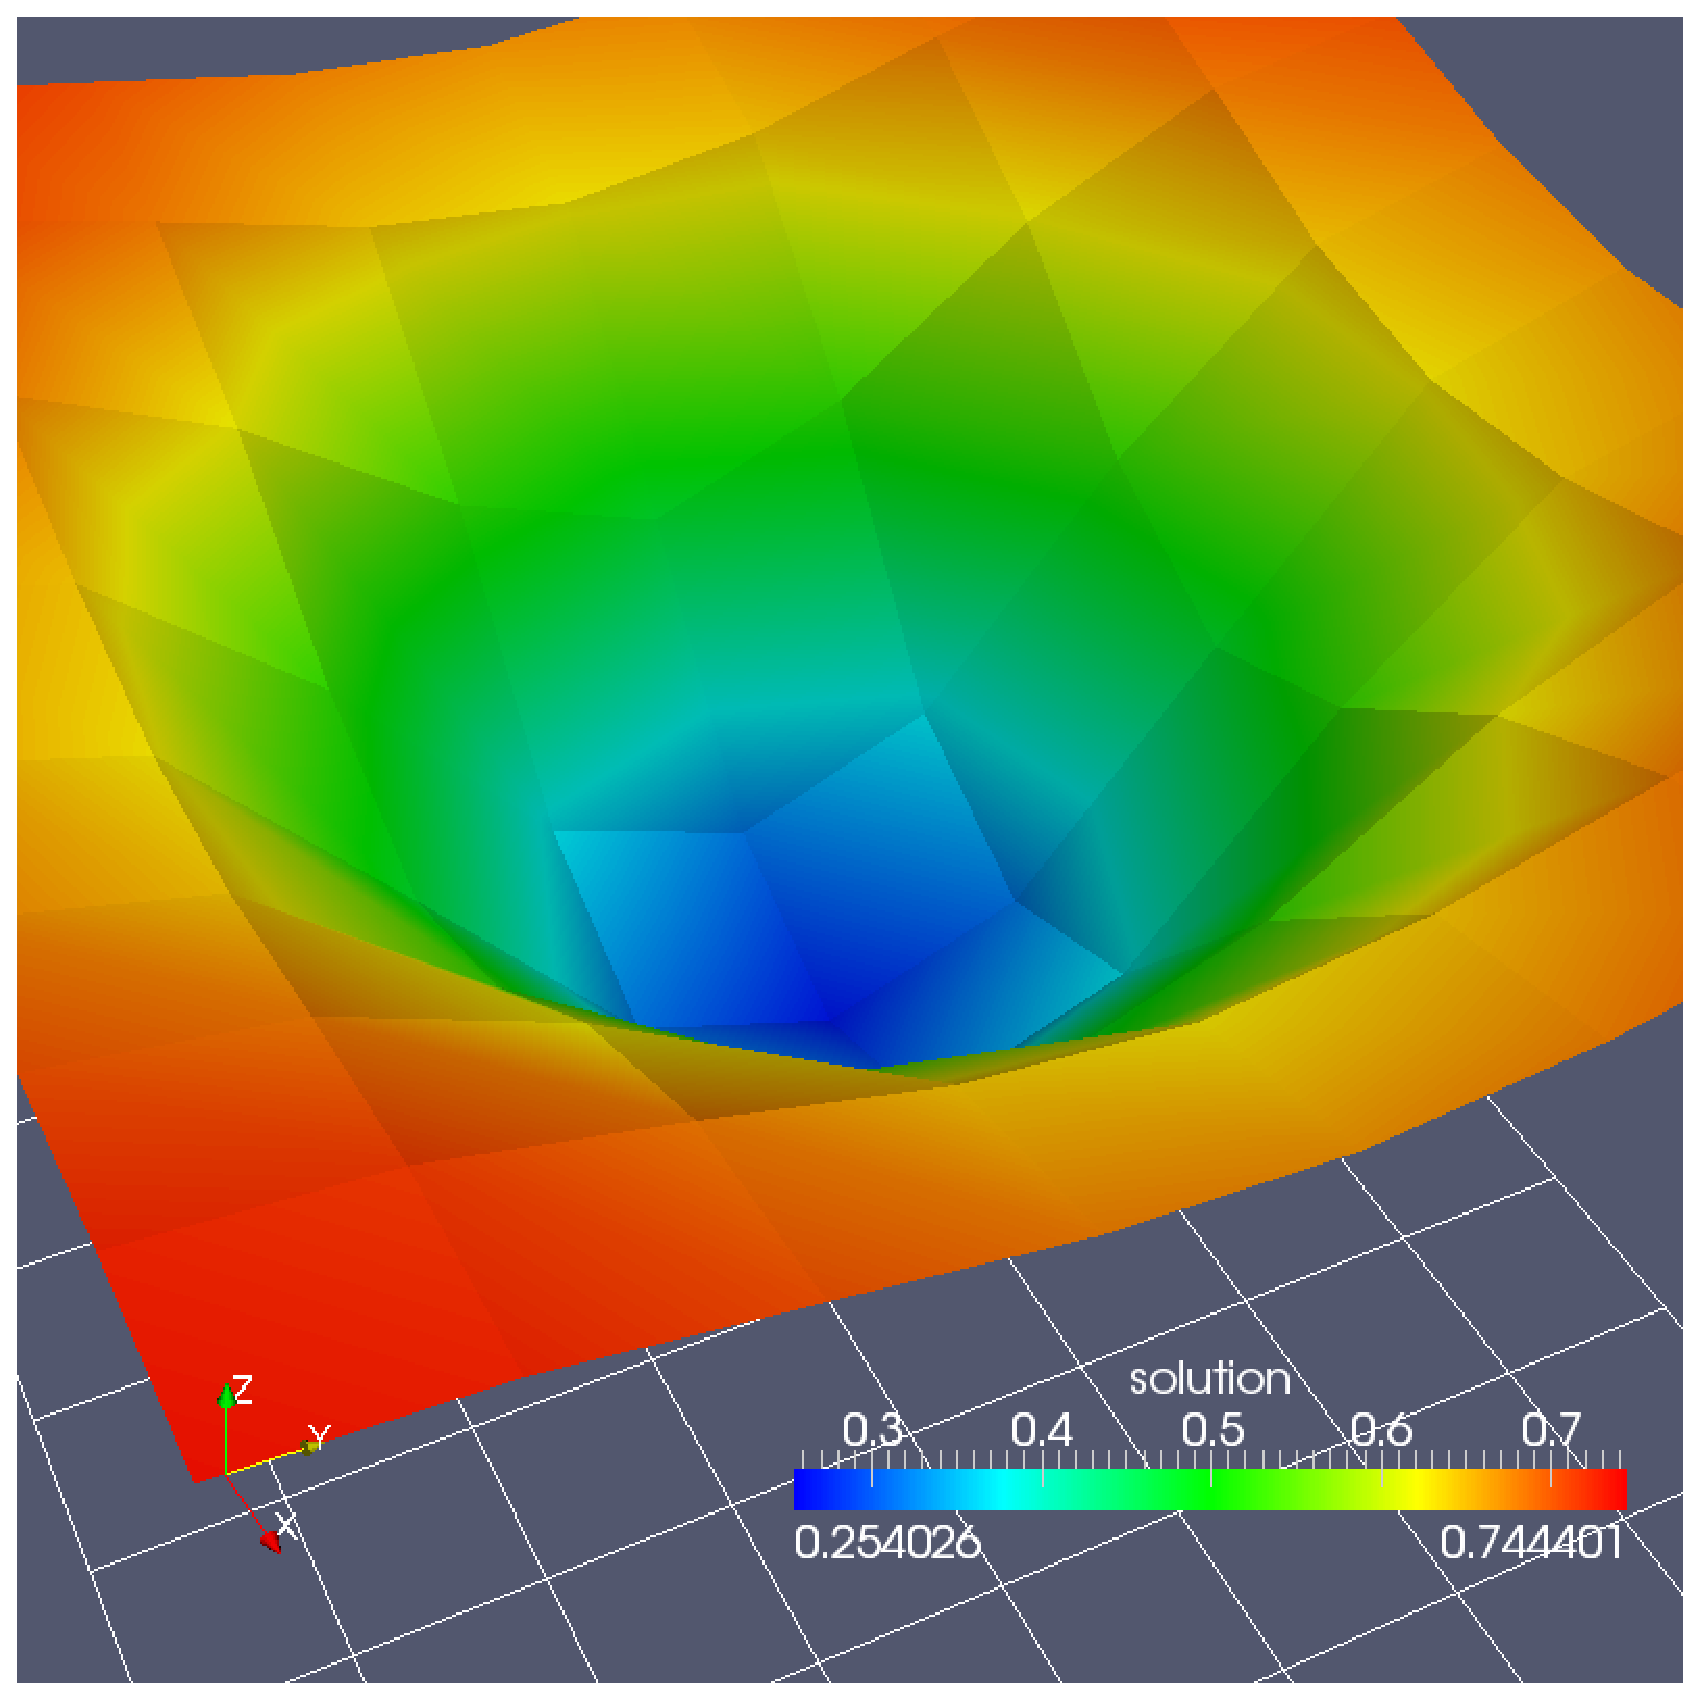
\includegraphics[width=0.32\textwidth]{./EPS/example01a_Q1} $\hspace{1mm}$
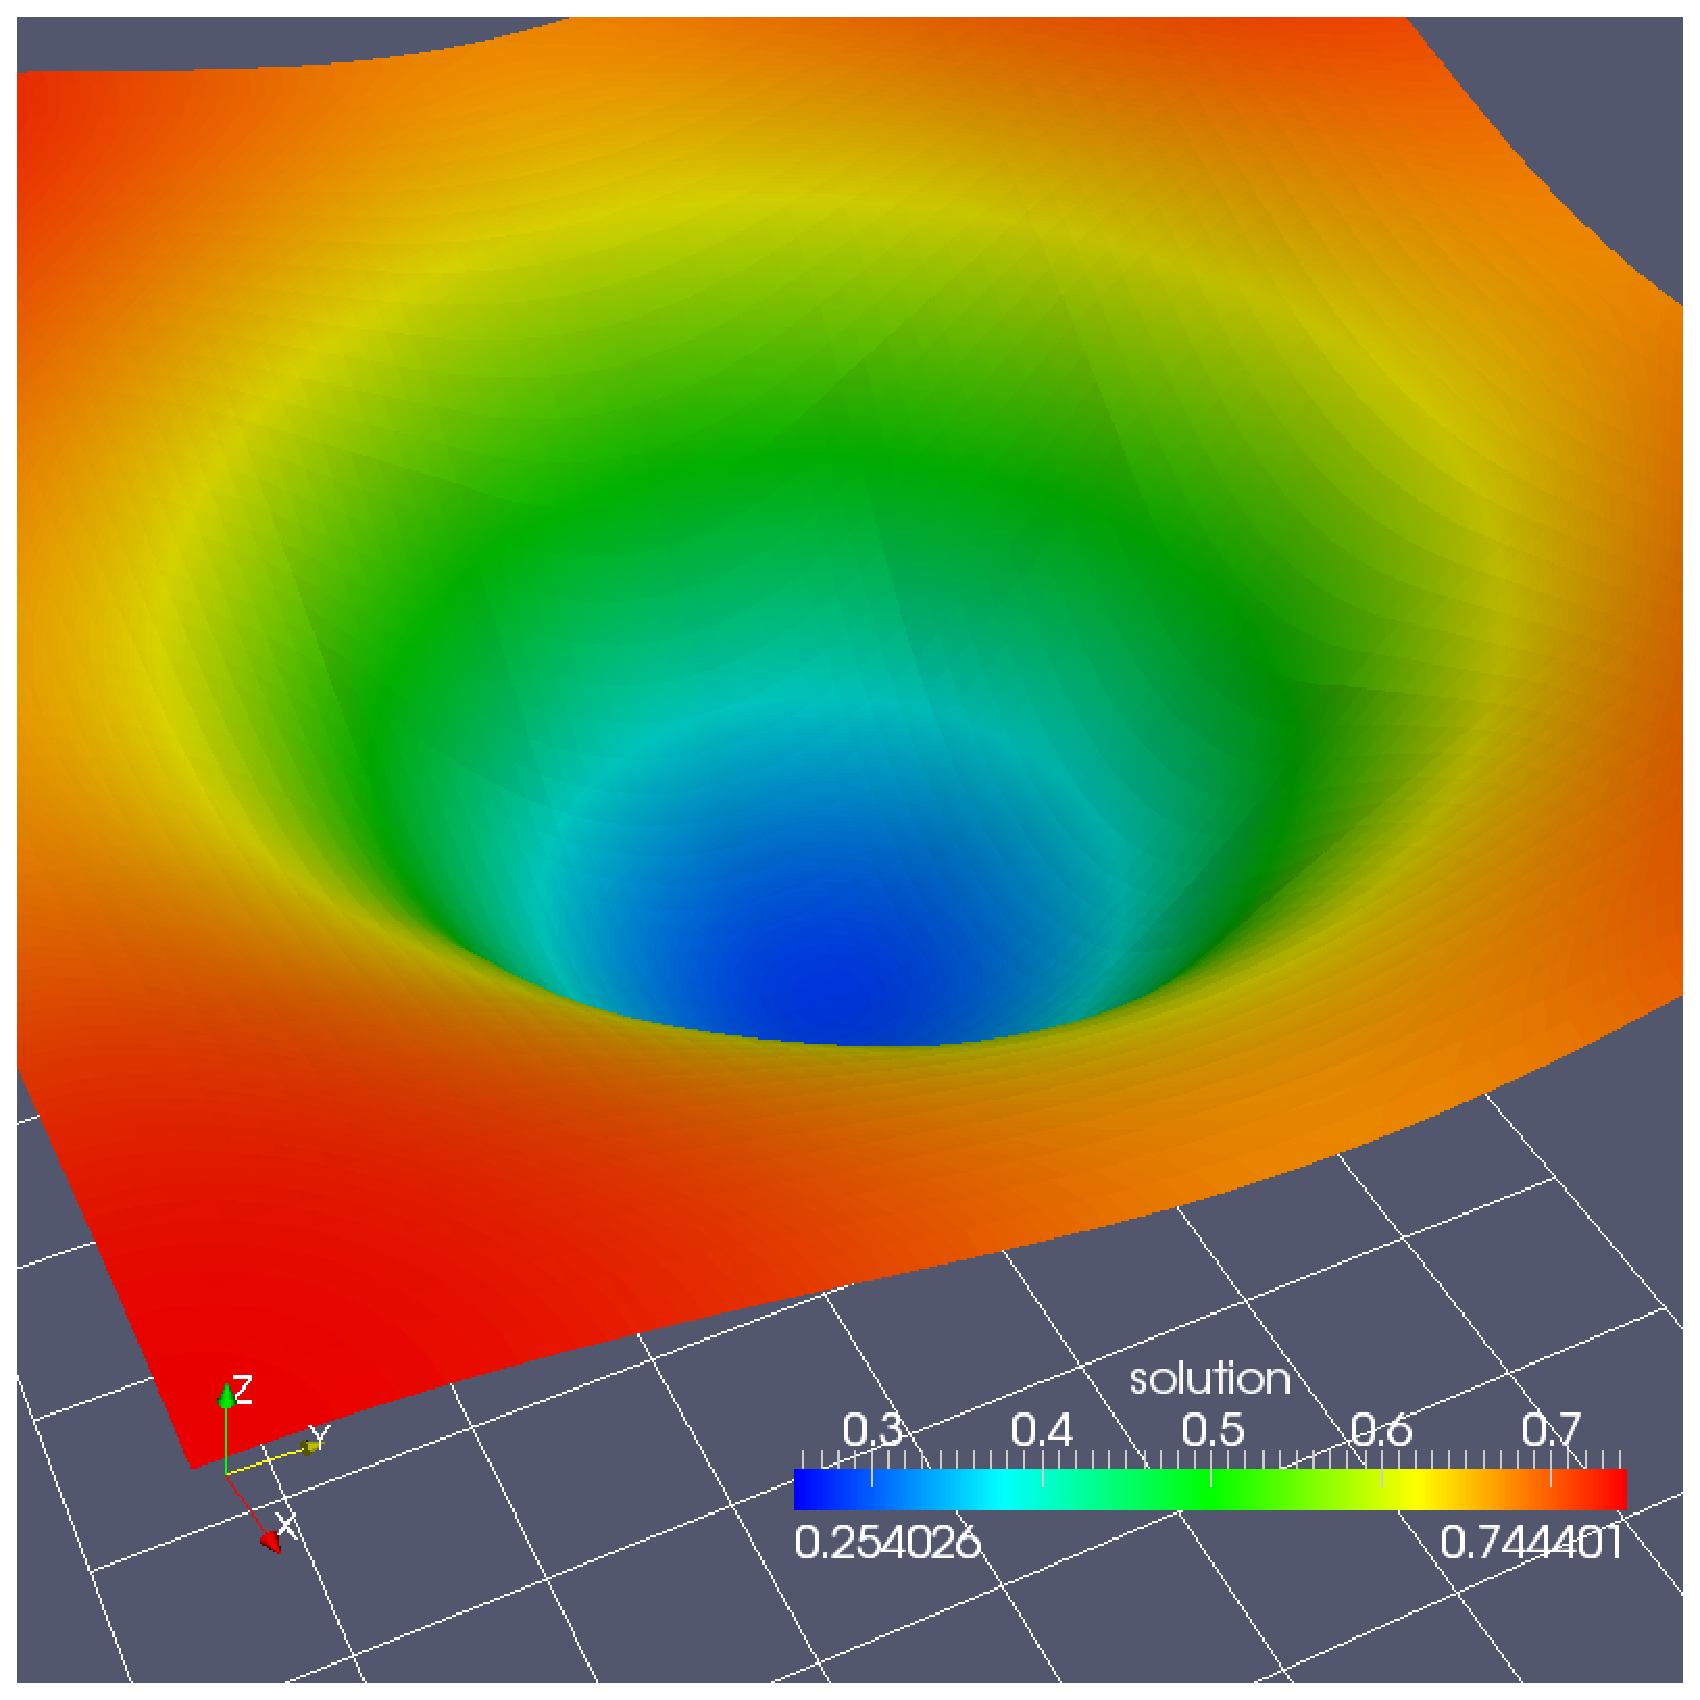
\includegraphics[width=0.32\textwidth]{./EPS/example01a_Q2} $\hspace{1mm}$
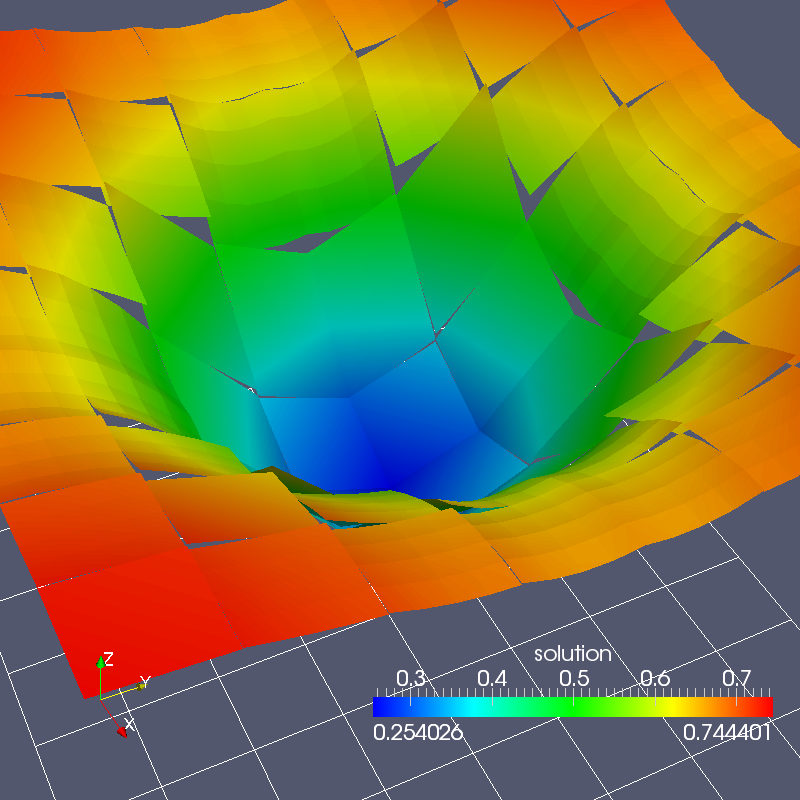
\includegraphics[width=0.32\textwidth]{./EPS/example01a_RT}
\end{center}
\caption{Results for example 1a computed with three different finite element spaces.
From left: $Q_1$ elements, $Q_2$ elements, rotated bilinear (Rannacher-Turek) element.}
\label{fig:Example01aResults}
\end{figure}
}


\begin{frame}
\frametitle{Using $Q_2$ Elements}
\ldots is quite simple, see \lstinline{example01a_Q2.hh}. Just
\begin{itemize}
\item Use another finite element map \lstinline{Q22DLocalFiniteElementMap}.
\item Increase quadrature order on the local operator to 4.
\item Use \lstinline{SubsamplingVTKWriter} to allow visualization of higher order polynomials.
\item Use a new name for the output file.
\end{itemize}

Explore the Rannacher Turek element in \lstinline{example01a_RT.hh}
\end{frame}


\begin{frame}<presentation>[fragile,allowframebreaks,allowdisplaybreaks]
\frametitle<presentation>{Unconstrained Elliptic Problem with $Q_2$}
\framesubtitle<presentation>{File \texttt{examples/example01a\_Q2.hh}}
\lstinputlisting[basicstyle=\ttfamily\tiny,numbers=left, 
numberstyle=\tiny, numbersep=2pt]{../../examples/example01a_Q2.hh}
\end{frame}
\mode<article>{
\begin{Lst}[File examples/example01a\_Q2.hh] \mbox
\nopagebreak
\lstinputlisting[basicstyle=\ttfamily\scriptsize,numbers=left, 
numberstyle=\tiny, numbersep=2pt]{../../examples/example01a_Q2.hh}
\end{Lst}}


\begin{frame}
\frametitle{Going Nonlinear}
\ldots is also easy. Just 
\begin{itemize}
\item Make a new local operator where the coefficients $a$ and $f$ depend on the solution $u$,
see \lstinline{example01b_operator}.
\item Use this new local operator in the grid operator space.
\item Use class \lstinline{Newton} to solve the nonlinear algebraic problem.
\item Use a new name for the output file :-).
\end{itemize}
\end{frame}

\begin{frame}<presentation>[fragile,allowframebreaks,allowdisplaybreaks]
\frametitle<presentation>{Unconstrained Nonlinear Elliptic Problem with $Q_2$}
\framesubtitle<presentation>{File \texttt{examples/example01b\_Q2.hh}}
\lstinputlisting[basicstyle=\ttfamily\tiny,numbers=left, 
numberstyle=\tiny, numbersep=2pt]{../../examples/example01b_Q2.hh}
\end{frame}
\mode<article>{
\begin{Lst}[File examples/example01b\_Q2.hh] \mbox
\nopagebreak
\lstinputlisting[basicstyle=\ttfamily\scriptsize,numbers=left, 
numberstyle=\tiny, numbersep=2pt]{../../examples/example01b_Q2.hh}
\end{Lst}}


\subsection{Constrained Elliptic Model Problem}

\begin{frame}
\frametitle{Problem and Weak Formulation}
Consider now the following model problem:
\begin{subequations} \label{Eq:Example02}
\begin{align*}
 -\Delta u + a u  &= f &&\text{in $\Omega\subset\mathbb{R}^d$},\\
                u &= g &&\text{on $\Gamma_D\subseteq\partial\Omega$},\\
-\nabla u \cdot n &= j &&\text{on $\Gamma_N=\partial\Omega\setminus\Gamma_D$},
\end{align*}
\end{subequations}
where $a>0$ when $\Gamma_D=\emptyset$.

Weak formulation. For $w\in H^1(\Omega)$, $w = g$ on 
$\Gamma_D$ (``extension of $g$''), set
\begin{align*}
\tilde{U} &= H_D^1(\Omega) = \{ u \in H^1(\Omega) \,:\, u|_{\Gamma_D}=0 \} \subset H^1(\Omega), \\
w + \tilde{U} &= \{ u \in H^1(\Omega) \,:\, u = w+\tilde{u} \wedge \tilde{u}\in\tilde{U}\},
\end{align*}

Then find
\begin{equation*}
u\in w+\tilde{U} \quad : \quad \underbrace{\int_\Omega \nabla u \cdot \nabla v + 
a u v - f v \,dx + \int_{\Gamma_N} j v \,ds}_{r(u,v)} = 0 \qquad \forall v\in\tilde{U}.
\end{equation*}
\end{frame}

\begin{frame}
\frametitle{What is different ?}
\begin{itemize}
\item The residual form has a new term which is a boundary integral.
\begin{itemize}
\item There will be an additional method on the local operator.
\end{itemize}
\item The problem is solved in an affine subspace. 
We call $\tilde{U}$ a \textit{constrained space}. 
\item In the linear case it suffices to solve a problem with homogeneous Dirichlet
boundary conditions:
\begin{subequations}
\begin{align*}
 -\Delta \bar{u} + a \bar{u}  &= f + \Delta w - a w &&\text{in $\Omega\subset\mathbb{R}^d$},\\
                \bar{u} &= 0 &&\text{on $\Gamma_D\subseteq\partial\Omega$},\\
-\nabla \bar{u} \cdot n &= j+\nabla w\cdot n &&\text{on $\Gamma_N=\partial\Omega\setminus\Gamma_D$},
\end{align*}
where $w$ is an extension of $g$ to $\Omega$ and $u = w + \bar{u}$.
\end{subequations}
\item In the nonlinear case this is not possible.
\end{itemize} 
\end{frame}


\begin{frame}
\frametitle{Finite Element Spaces in Constrained Case}
\begin{itemize}
\item Define appropriate finite-dimensional subspaces:
\begin{equation*}
\tilde{U}_h^k = \left \{ u \in U_h^k \,:\, u|_{\Gamma_D} = 0 \right\} \subset U_h^k.
\end{equation*}
(Mesh resolves the Dirichlet bopundary $\Gamma_D$.
\item Provide extension $w\in U_h^k$ with ``$w=g$'' on $\Gamma_D$ in an appropriate sense.
\item Obviously, $\text{dim}\tilde{U}_h^k < \text{dim} U_h^k$.
\item Note: Dirichlet boundary conditions could also be handled by penalty methods. 
This can be done easily in PDELab but is not shown here. 
\end{itemize}
\end{frame}

\begin{frame}
\frametitle{Realization of Dirichlet Constraints}
\begin{itemize}
\item Assume $\Phi_{U_h^k}$ is a Lagrange basis: 
\begin{equation*}
\phi_j(x_i)=\delta_{i,j} \quad\text{where $x_i$ are the Lagrange points}.
\end{equation*}
\item Construct subspace via basis representation:
\begin{itemize}
\item $\mathcal{I}_{\tilde{U}_h^k} = \left\{ j\in \mathcal{I}_{U_h^k} \,:\, 
x_j \not\in \Gamma_D \right\} \subset \mathcal{I}_{U_h^k}$.
\item $\Phi_{\tilde{U}_h^k} = \left\{ \phi_j\in \Phi_{U_h^k} \,:\, 
j \in \mathcal{I}_{\tilde{U}_h^k} \right\} \subset \Phi_{U_h^k}$.
\item $\tilde{U}_h^k = \text{span}\Phi_{\tilde{U}_h^k}$.
\end{itemize}
\item For the coefficient space there are two options:
\begin{enumerate}
\item $\tilde{\mathbf{U}} = \mathbb{R}^{\mathcal{I}_{\tilde{U}_h^k}} \not\subseteq \mathbf{U}$.
\item $\tilde{\mathbf{U}} = \left\{ \mathbf{u}\in\mathbf{U} \,:\, (\mathbf{u})_j = 0 \  \forall
j \in \mathcal{I}_{U_h^k} \setminus \mathcal{I}_{\tilde{U}_h^k} \right\} \subset \mathbf{U}$. 
\end{enumerate}
\item We choose (2) because
\begin{itemize}
\item $w + \tilde{u}$ is just adding coefficient vectors.
\item Changing $\Gamma_D$, e.g. in time-dependent problems is easy.
\end{itemize}
\end{itemize}
\end{frame}


\begin{frame}
\frametitle{General Constrained Spaces}
\begin{itemize}
\item Constrained spaces turn up in a number of other cases:
\begin{itemize}
\item Hanging nodes.
\item Functions with zero average, rigid body modes.
\item Varying polynomial degree in conforming finite elements ($p$-method).
\item Periodic boundary conditions.
\item Artificial essential boundary conditions or ghost degrees of freedom in parallelization.
\end{itemize}
\item PDELab has a general concept to handle all types of constraints. 
\item Given $U_h$ with index set $\mathcal{I}_{U_h^k}$, construct a basis of the subspace:
\begin{itemize}
\item Partition index set: $\mathcal{I}_{U_h^k} = \tilde{\mathcal{I}} \cup \bar{\mathcal{I}}$.
\item Construct new basis from given basis:
\begin{equation*}
\tilde\phi_i = \phi_i + \sum\limits_{j\in\bar{\mathcal{I}}} \omega_{i,j} \phi_j, \qquad i\in\tilde{\mathcal{I}}.
\end{equation*}
\item $\tilde{U}_h$ is spanned by the new basis.
\end{itemize}
\item Constrained space defined by splitting $\tilde{\mathcal{I}} \cup \bar{\mathcal{I}}$ 
and coefficients $\omega_{i,j}$.
\end{itemize}
\end{frame}


\subsection{Example 2}

\begin{frame}
\frametitle{Example 2 Overview}
The first example implements model problem \eqref{Eq:Example01}.

It consists of the following files:
\begin{itemize}
\item \lstinline{example02.cc} -- the file to be compiled, main function. 
\item \lstinline{example02_bctype.hh} -- a function giving the splitting $\partial\Omega = \Gamma_D \cup \Gamma_N$.
\item \lstinline{example02_bcextension.hh} -- a function for $g$ and its extension $w$.
\item \lstinline{example02_operator.hh} -- local operator including inhomogeneous Neumann boundary conditions.
\item \lstinline{example02_Q1.hh} -- driver setting up and solving the problem. 
\end{itemize}
\end{frame}

\begin{frame}
\frametitle{Driver for Solving Constrained Linear Problem}
\framesubtitle{About \lstinline{example02_Q1.hh}}
\begin{itemize}
\item Class \lstinline{ConformingDirichletConstraints} parametrizes the grid function space
with the possibility of having Dirichlet constraints.
\item Function \lstinline{constraints} assembles constraints (i.e. the splitting 
$\mathcal{I}_{U_h^k} = \tilde{\mathcal{I}} \cup \bar{\mathcal{I}}$) from a given function.
\item Function \lstinline{interpolate} initializes a coefficient vector from a given function.
At the same time this defines the extension $w$ of $g$.
\item The rest is the same as before.
\end{itemize}
\end{frame}

\begin{frame}<presentation>[fragile,allowframebreaks,allowdisplaybreaks]
\frametitle<presentation>{Constrained Elliptic Problem}
\framesubtitle<presentation>{File \texttt{examples/example02\_Q1.hh}}
\lstinputlisting[basicstyle=\ttfamily\tiny,numbers=left, 
numberstyle=\tiny, numbersep=2pt]{../../examples/example02_Q1.hh}
\end{frame}
\mode<article>{
\begin{Lst}[File examples/example02\_Q1.hh] \mbox
\nopagebreak
\lstinputlisting[basicstyle=\ttfamily\scriptsize,numbers=left, 
numberstyle=\tiny, numbersep=2pt]{../../examples/example02_Q1.hh}
\end{Lst}}

\begin{frame}<presentation>[fragile,allowframebreaks,allowdisplaybreaks]
\frametitle<presentation>{Boundary Condition Type Function}
\framesubtitle<presentation>{File \texttt{examples/example02\_bctype.hh}}
\lstinputlisting[basicstyle=\ttfamily\tiny,numbers=left, 
numberstyle=\tiny, numbersep=2pt]{../../examples/example02_bctype.hh}
\end{frame}
\mode<article>{
\begin{Lst}[File examples/example02\_bctype.hh] \mbox
\nopagebreak
\lstinputlisting[basicstyle=\ttfamily\scriptsize,numbers=left, 
numberstyle=\tiny, numbersep=2pt]{../../examples/example02_bctype.hh}
\end{Lst}}

\begin{frame}<presentation>[fragile,allowframebreaks,allowdisplaybreaks]
\frametitle<presentation>{Boundary Condition Extension Function}
\framesubtitle<presentation>{File \texttt{examples/example02\_bcextension.hh}}
\lstinputlisting[basicstyle=\ttfamily\tiny,numbers=left, 
numberstyle=\tiny, numbersep=2pt]{../../examples/example02_bcextension.hh}
\end{frame}
\mode<article>{
\begin{Lst}[File examples/example02\_bcextension.hh] \mbox
\nopagebreak
\lstinputlisting[basicstyle=\ttfamily\scriptsize,numbers=left, 
numberstyle=\tiny, numbersep=2pt]{../../examples/example02_bcextension.hh}
\end{Lst}}

\begin{frame}[fragile]
\frametitle{\lstinline{alpha_boundary} Method}
Local operator is extended by a new method \lstinline{alpha_boundary}
computing the boundary integral.

\lstinline{alpha_boundary} has the following signature: 
\begin{lstlisting}[basicstyle=\ttfamily\scriptsize]
template<typename IG, typename LFSU, typename X, 
         typename LFSV, typename R>
void alpha_boundary (const IG& ig, const LFSU& lfsu_s, const X& x_s, 
                     const LFSV& lfsv_s, R& r_s) const
\end{lstlisting}
Where the arguments are:
\begin{itemize}
\item \lstinline{ig} -- intersection with domain boundary.
\item \lstinline{lfsu_s} -- local basis $\hat\phi_{e,l}$ for trial space on inside element.
\item \lstinline{x_s} -- local coefficients on inside element.
\item \lstinline{lfsv_s} -- local basis $\hat\psi_{e,l}$ for test space on inside element. 
\item \lstinline{r_s} -- local contribution to residual on inside element.
\end{itemize}
\end{frame}


\begin{frame}<presentation>[fragile,allowframebreaks,allowdisplaybreaks]
\frametitle<presentation>{Local Operator with Neumann Boundary}
\framesubtitle<presentation>{File \texttt{examples/example02\_operator.hh}}
\lstinputlisting[basicstyle=\ttfamily\tiny,numbers=left, 
numberstyle=\tiny, numbersep=2pt]{../../examples/example02_operator.hh}
\end{frame}
\mode<article>{
\begin{Lst}[File examples/example02\_operator.hh] \mbox
\nopagebreak
\lstinputlisting[basicstyle=\ttfamily\scriptsize,numbers=left, 
numberstyle=\tiny, numbersep=2pt]{../../examples/example02_operator.hh}
\end{Lst}}

\begin{frame}<presentation>
\frametitle{Visualization of Example 2 Results}
Neumann boundary condition at $x=1$, Dirichlet elsewhere.

\begin{center}
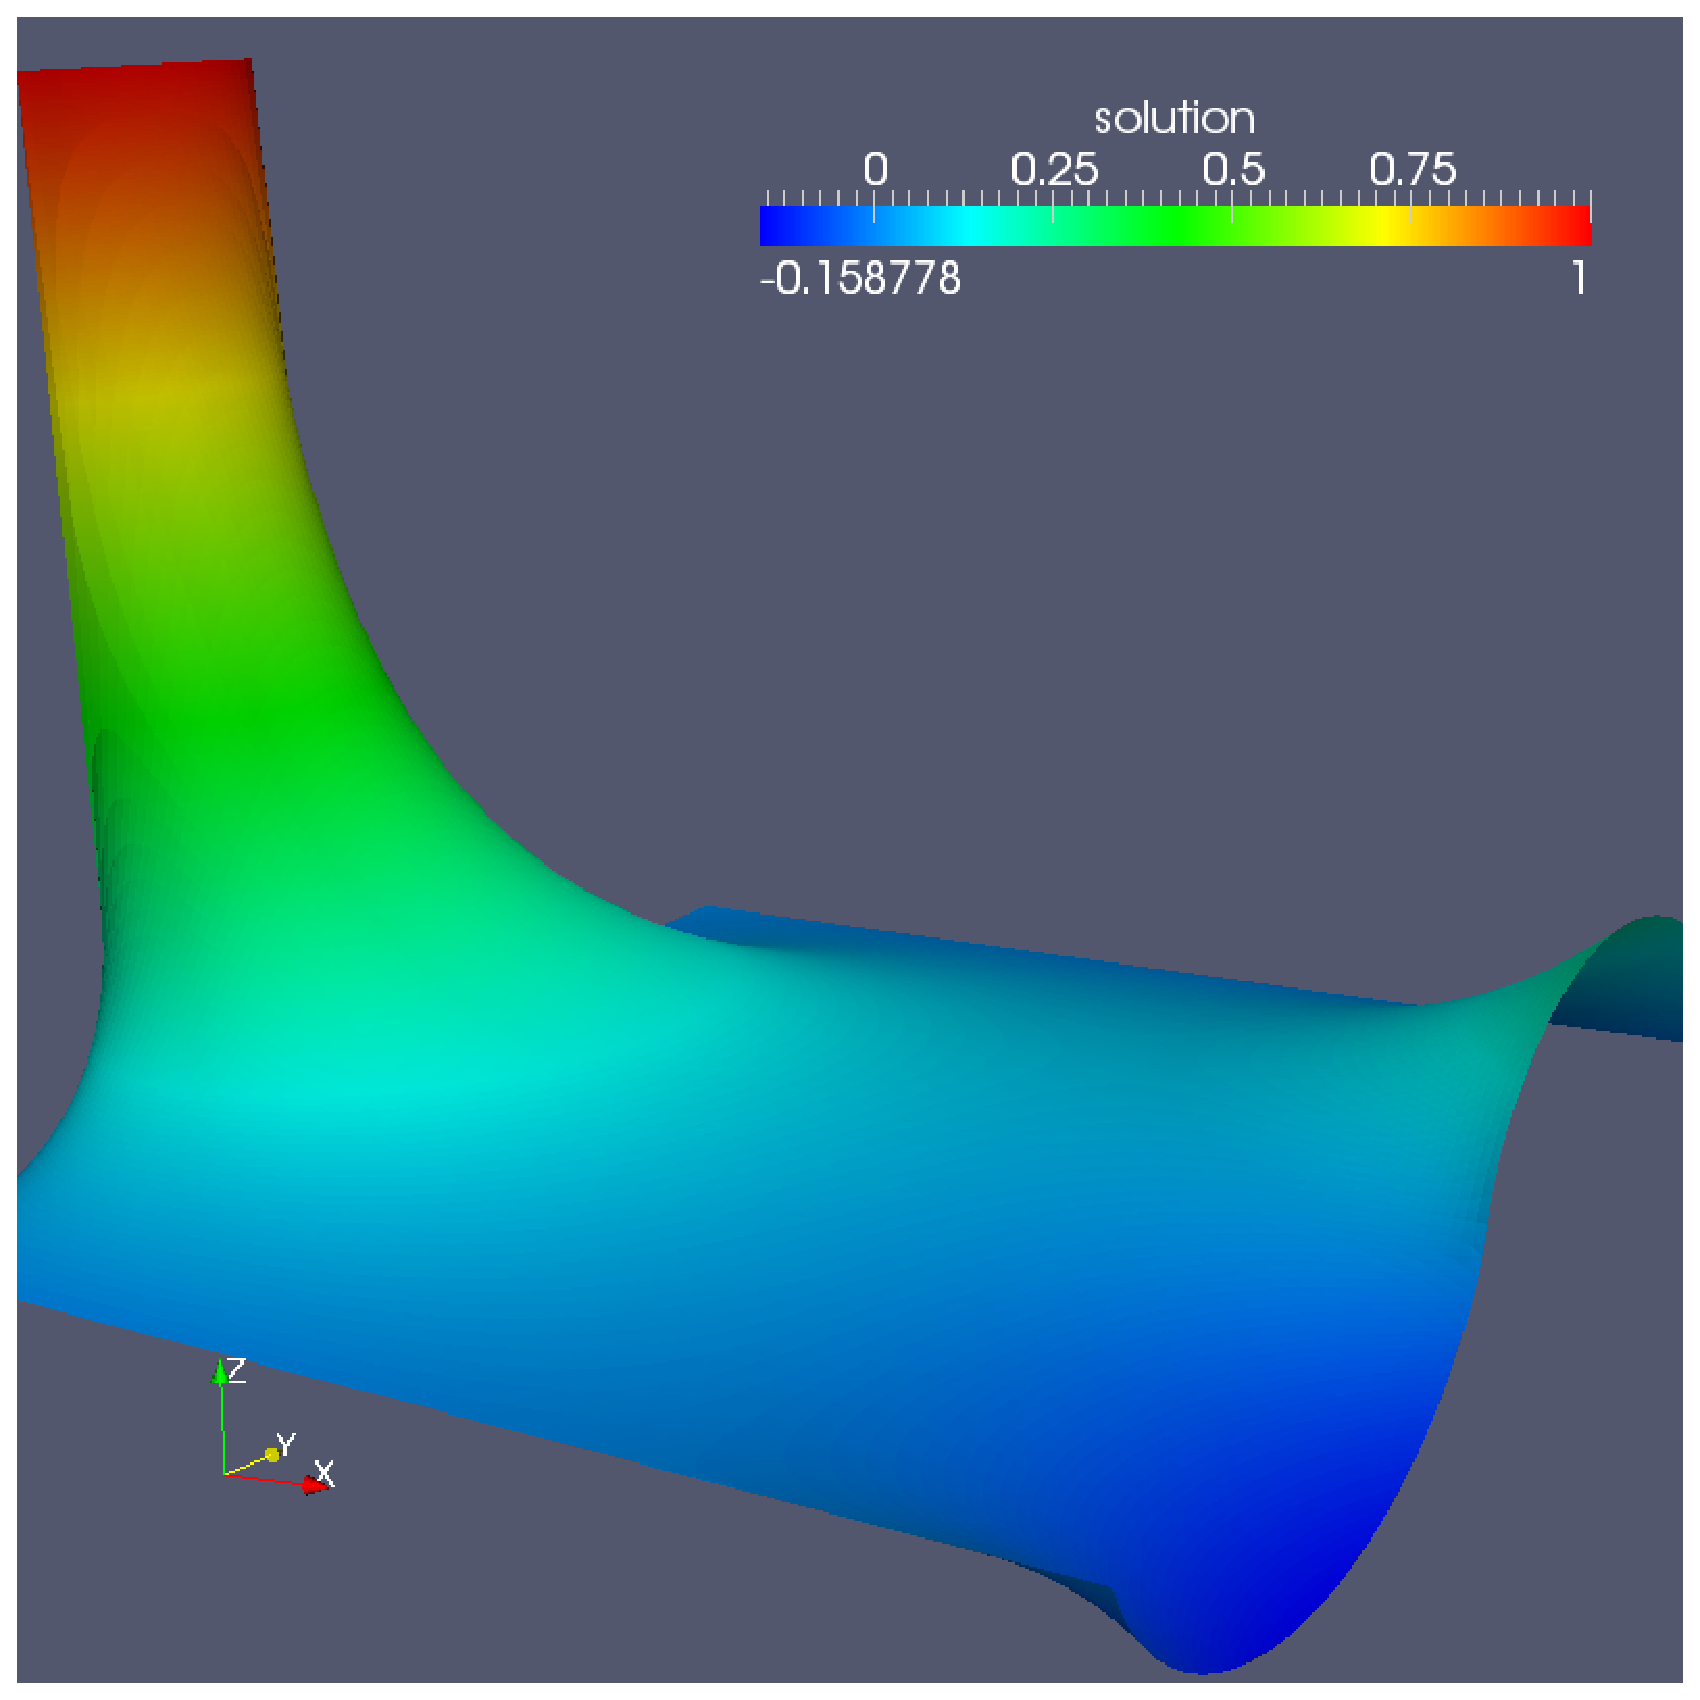
\includegraphics[width=0.58\textwidth]{./EPS/example02_Q1}
\end{center}
\end{frame}

\mode<article>{
Figure \ref{fig:Example01aResults} shows visualizations of the results computed
with \lstinline{example01}.
\begin{figure}
\begin{center}
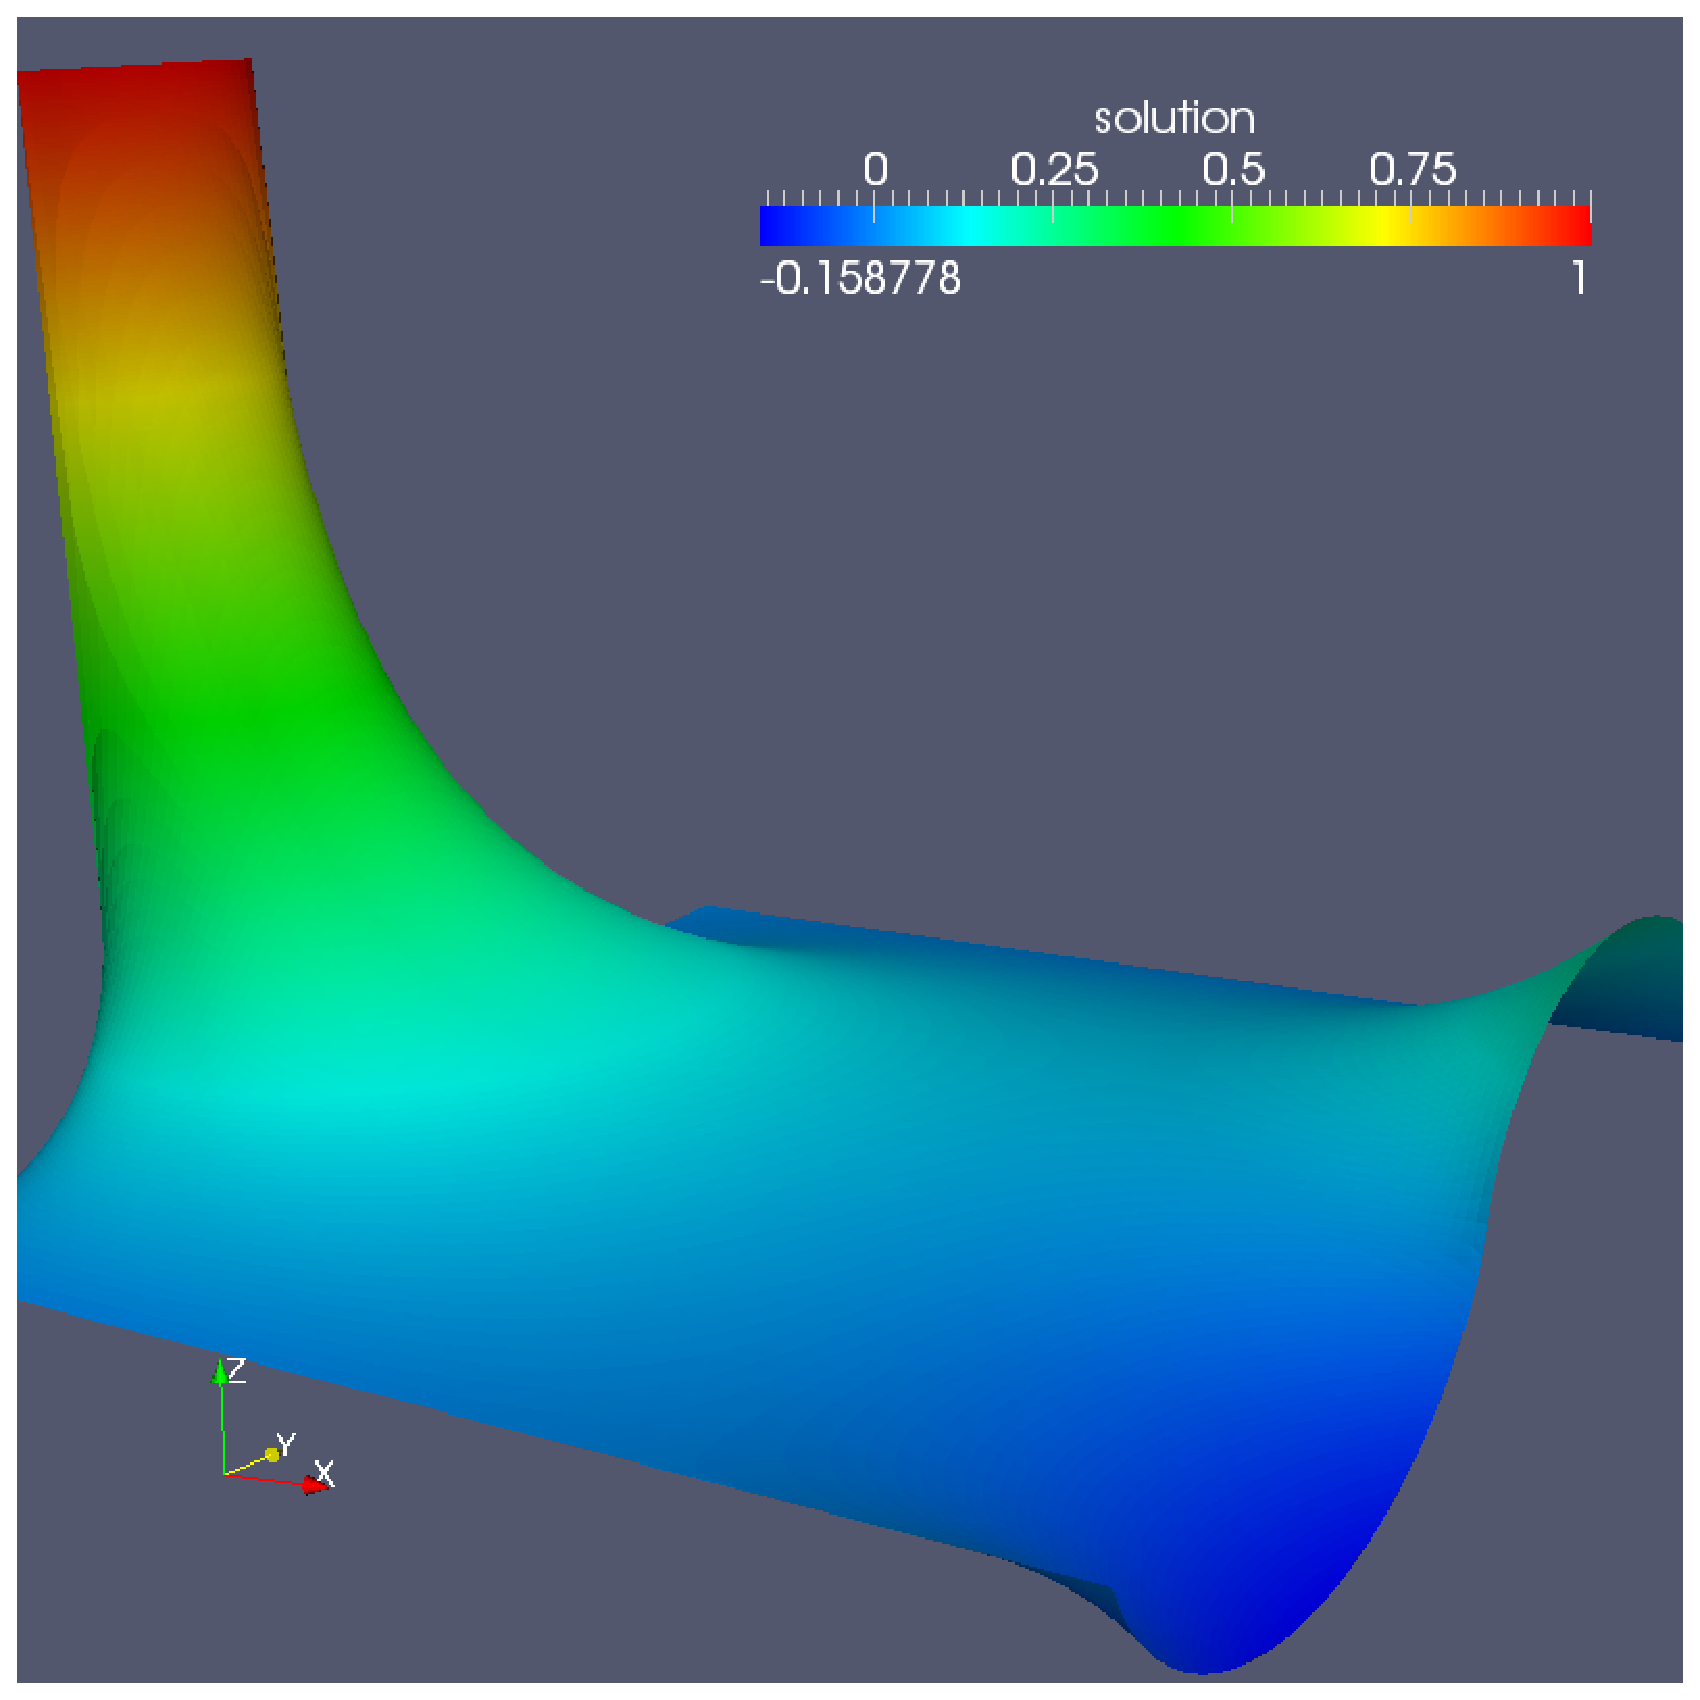
\includegraphics[width=0.5\textwidth]{./EPS/example02_Q1}
\end{center}
\caption{Result for example 2 computed with $Q_1$ elements.}
\label{fig:Example02Results}
\end{figure}
}

\begin{frame}
\frametitle{Remark on Local Operators}
In practice one would access parameter functions such as $a, f, j$ and the boundary condition
type from the implementation of the local operator.
\end{frame}


\subsection{Cell-centered Finite Volumes}

\subsection{Example 4}

}
\mode<all>{{
\lstset{breakatwhitespace=true,breaklines=true}
\section{PDELab backends}
\label{sec:pdelab-backends}

\begin{frame}
  \frametitle<presentation>{PDELab backend}
  \begin{itemize}
  \item Linear algebra is decoupled from the discretization.
  \item Provides unique access interface for matrices, vectors and
    solvers.
  \item (Often) easily extensible for use of other libraries.
  \item Minimal knowledge of the underlying libraries required.
  \end{itemize}
\end{frame}

\begin{frame}
  \frametitle{PDELab backend in UML}
  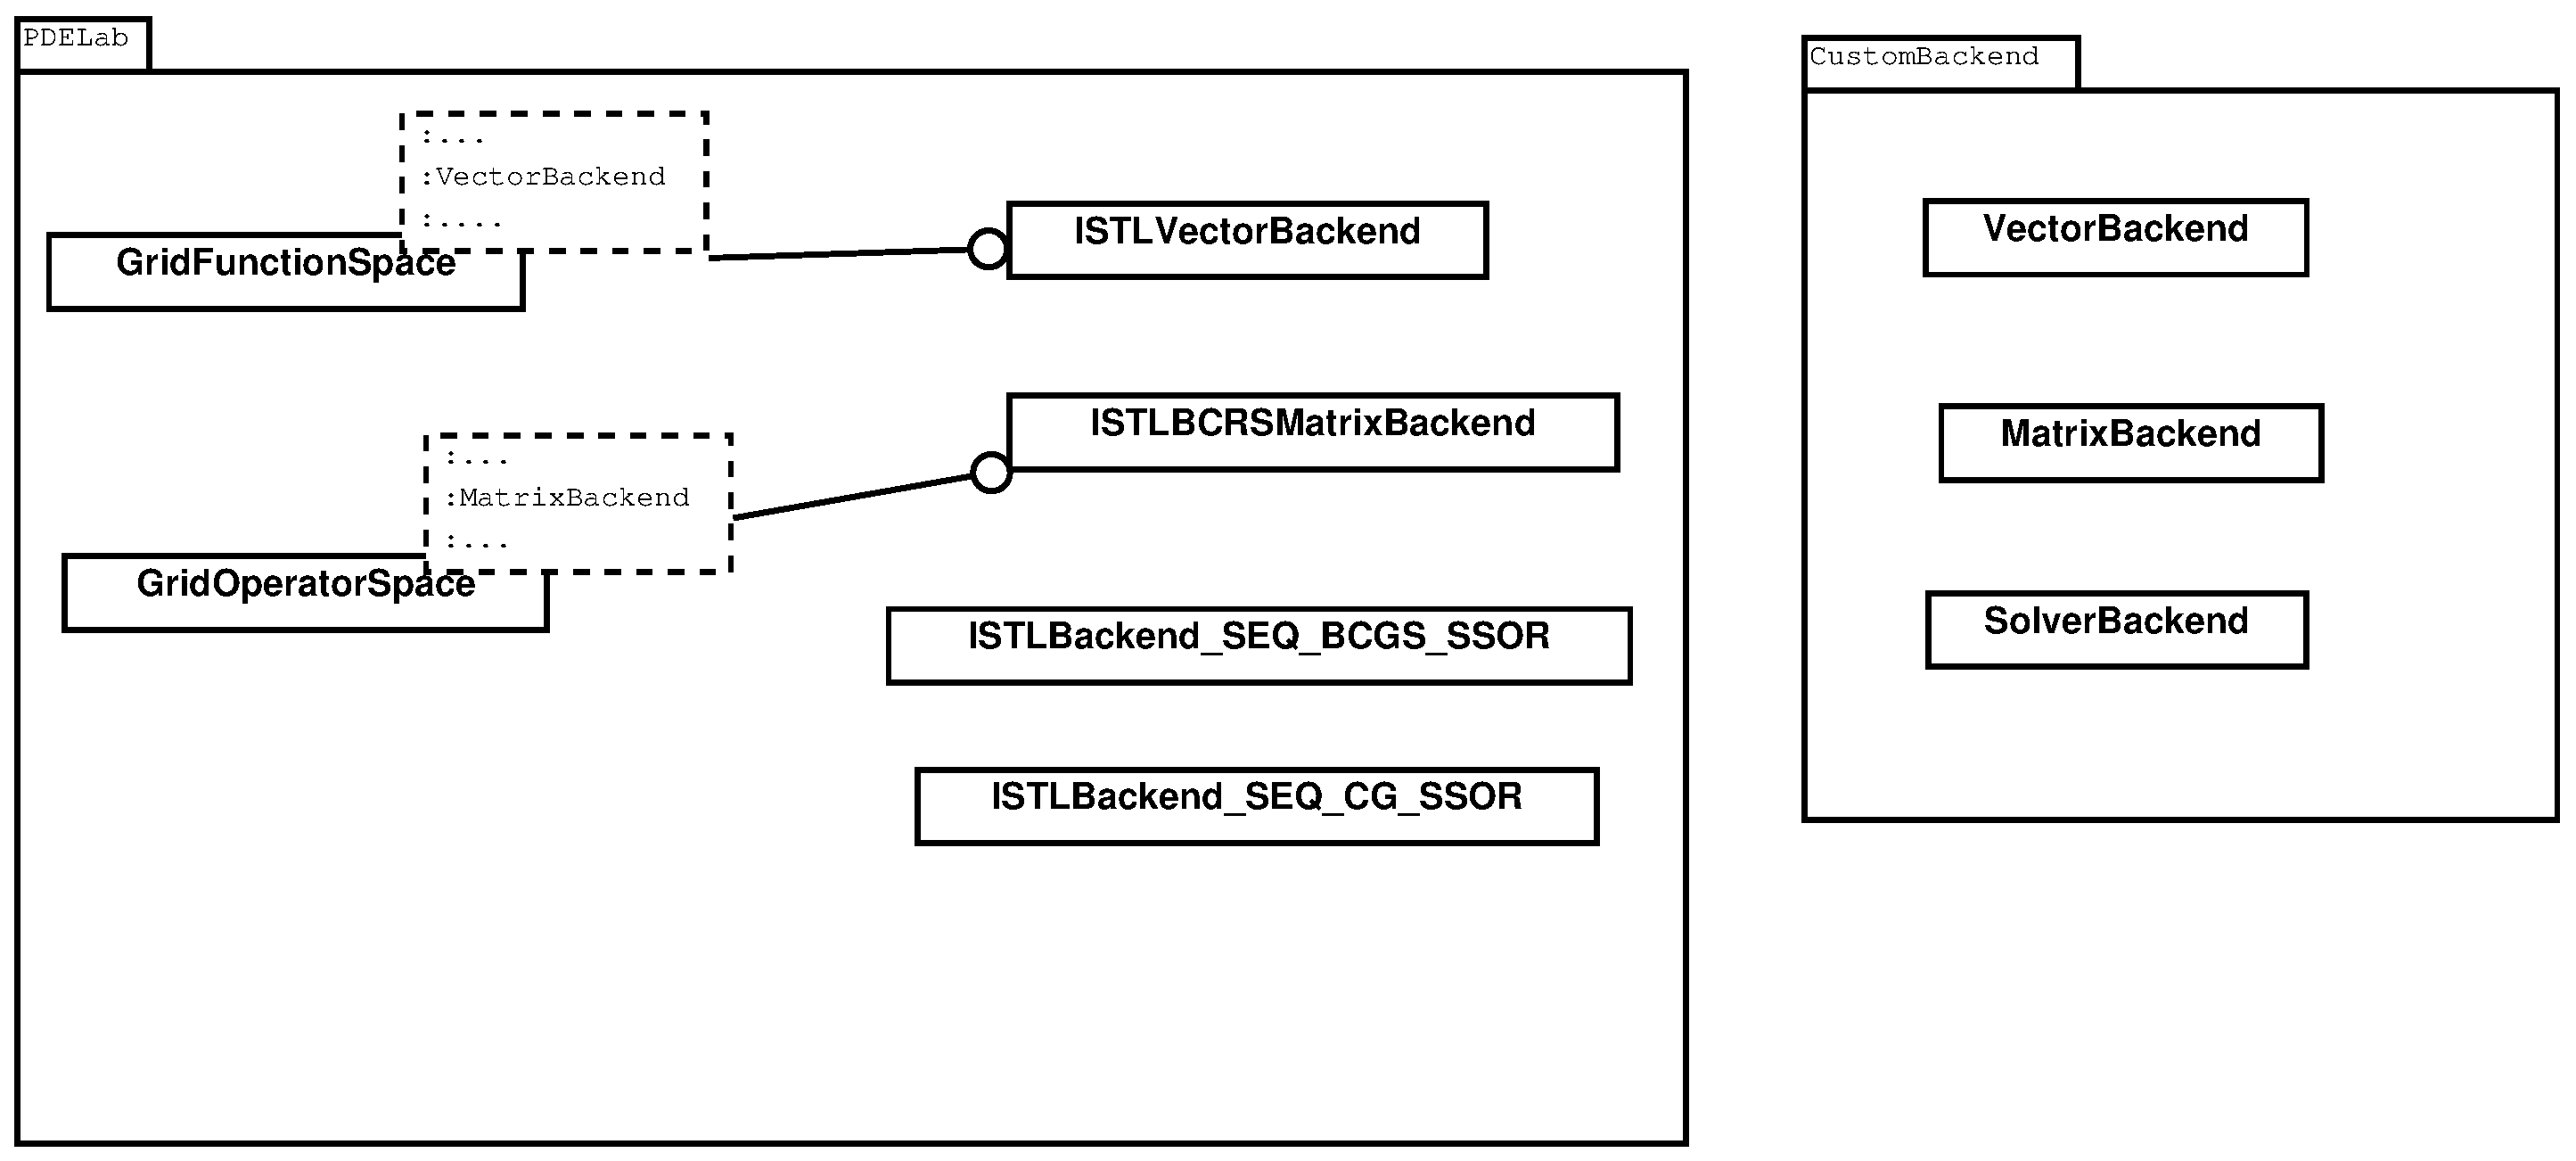
\includegraphics[width=\textwidth]{./EPS/backend}
\end{frame}
\subsection{Interface}
\label{sec:interface}

\subsubsection{The Vector Backend}
\label{sec:vector-backend}

\begin{frame}
  \frametitle<presentation>{The Vector Backend}
  \begin{itemize}
  \item It is a class not a namespace to allow template parameterization!
  \item Provides the actual container type as
    \lstinline!template<class T, class E> Vector!.
  \item Associated type \lstinline!size_type! used for index access.
  \item Const and mutable data access with 
    \lstinline!access(Vector<T,E>& cont, size_type i)!
  \end{itemize}
\end{frame}

\begin{frame}[fragile]
  \frametitle{Sample Vector Container}
  \begin{itemize}
  \item Template parameter T is the type of the grid function used.
  \item Template parameter E is the value type (e.g. double, float).
  \end{itemize}
  \begin{lstlisting}[basicstyle=\scriptsize]
    template<typename T, typename E>
    class VectorContainer 
    {
      public:
      // The stored element type
      typedef E ElementType;
      // The backend we are associated with
      typedef ISTLVectorBackend<BLOCKSIZE> Backend;
      
      //constructor with grid function space t
      VectorContainer (const T& t_);

      //constructor with grid function space t, initial value e
      VectorContainer (const T& t_, const E& e);
      
      // assignment
      VectorContainer& operator= (const E& e);
    };
  \end{lstlisting}
\end{frame}
\subsubsection{The Matrix Backend}
\label{sec:vector-backend}

\begin{frame}
  \frametitle<presentation>{The Matrix Backend}
  \begin{itemize}
  \item It is a class not a namespace to allow template
    parameterization!
  \item Provides the actual container type as
    \lstinline!template<class T, class E> Matrix!.
%  \item Provides associated type \lstinline!Pattern! for setting up
%    the sparsity pattern.
  \item Provides method \lstinline!clearRow(RI i, C& c)! for setting
    the values of row with index $i$ of container \lstinline!c! to zero.
  \end{itemize}
\end{frame}

\begin{frame}[fragile]
  \frametitle{The Matrix Container}
\begin{itemize}
  \item Template parameter T is the type of the grid function used.
  \item Template parameter E is the value type (e.g. double, float).
  \end{itemize}
  \begin{lstlisting}[basicstyle=\scriptsize]
template<class T, class E>
class MatrixContainer{
  public:
    // The stored element type
    typedef typename E ElementType;
    // The backend we are associated with
    typedef ISTLMatrixBackend<ROWBLOCKSIZE,COLBLOCKSIZE> Backend;
      
    //constructor with grid operator space t
    // Needs to setup the whole sparsity pattern.
    MatrixContainer (const T& t_);
      
    // assignment
    MatrixContainer& operator= (const E& e);
};
  \end{lstlisting}
\end{frame}
\begin{frame}[fragile]
  \frametitle{Sparse Matrix Setup in PDELab}
  \begin{itemize}
  \item Setting up a sparse matrix is a two step procedure:
    \begin{enumerate}
    \item Setting up the sparsity pattern.
    \item Filling the matrix with the values.
    \end{enumerate}
  \item First step is performed by the contructor of the matrix
    container.
  \item Second step is performed by the member function
    \lstinline!jacobian! of the grid operator space.
  \end{itemize}

\end{frame}

\subsubsection{The Linear Solver Backend}
\label{sec:line-solv-back}

\begin{frame}[fragile]
  \frametitle<presentation>{The Linear Solver Backend}
  \begin{itemize}
  \item Provides vector norm method needed by nonlinear PDELab solvers:
      \begin{lstlisting}
template<class V>
typename V::ElementType norm(const V& v) const;
      \end{lstlisting}
    \item Member function \lstinline!result()! returns statistics
      about the solution phase in an instance of the
      \lstinline!template<class T> LinearSolverResult! class template.
\item Use member function 
  \begin{lstlisting}
template<class M.class V,class W>
apply(M& A, V& z, W& r, typename V::ElementType reduction);
  \end{lstlisting}
  to (iteratively) solve $Az=r$ until the prescribed relative defect
  reduction is achieved.
  \item For ISTL it hides a lot of the compexity that heavy usage of
    templates imposes on the user.
  \end{itemize}
\end{frame}

\subsection{The Iterative Solver Template Library}
\label{sec:iter-solv-templ}

\subsubsection{Block Structure in FE Matrices}
\label{sec:motivation}
\begin{frame} \frametitle{PDE Systems}
  \begin{block}{}
      We have several unknowns and therefore several grid functions
      when dealing with PDE Systems.
      For the simple case that each function has the same structure we
      can use the following special ordering and blocking approaches:
  \begin{itemize}
  \item Equation-wise blocking: All degrees of freedom associated with
    the same unknown are blocked together.
  \item Point-wise blocking: All degrees of freedom associated with
    the same point (or element) are blocked together.
  \item No blocking is used.
  \end{itemize}
  \end{block}
  Currently the last two approaches are supported by PDELab with the
  ISTL backend.
\end{frame}
In the pictures below the degrees of freedom are visualized using
circles at the positions/entities they are associated with. Circles
with the same colour are blocked together. In the the entries in the
resulting matrix are dense and sparse matrices for the equation-wise
and point-wise blocking, respectively.
\begin{frame}
\frametitle{Some Examples for Block Structure}
\begin{block}{}
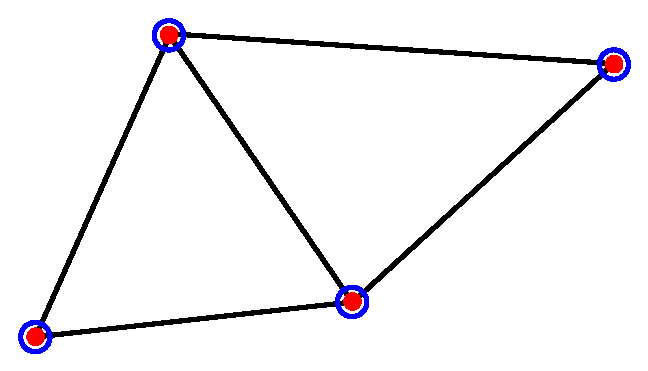
\includegraphics[width=0.48\textwidth]{./EPS/P1P1}\hfill
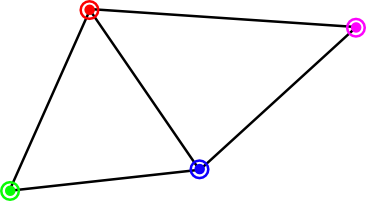
\includegraphics[width=0.48\textwidth]{./EPS/P1P1b}

\begin{minipage}{0.48\textwidth}
\centering $P_1\times P_1$ equation-wise
\end{minipage}
\begin{minipage}{0.48\textwidth}
\centering $P_1\times P_1$ point block
\end{minipage}

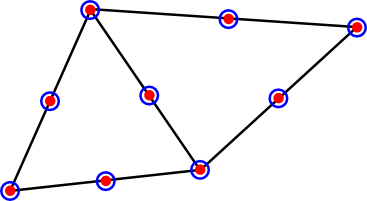
\includegraphics[width=0.48\textwidth]{./EPS/P2P2}\hfill
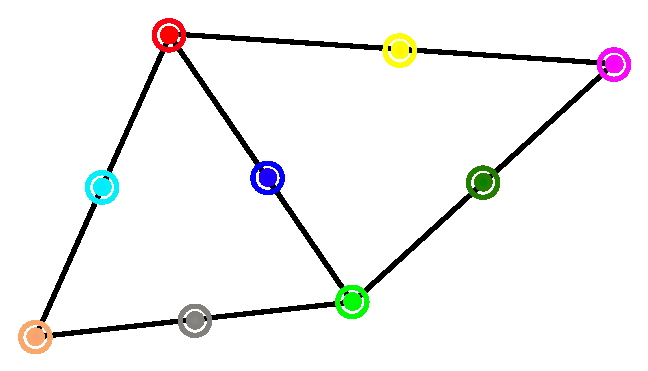
\includegraphics[width=0.48\textwidth]{./EPS/P2P2b}

\begin{minipage}{0.48\textwidth}
\centering $P_2\times P_2$ equation-wise
\end{minipage}
\begin{minipage}{0.48\textwidth}
\centering $P_2\times P_2$ point block
\end{minipage}
\end{block}
\end{frame}

\subsubsection{Matrix Vector Components}
\label{sec:matr-vect-comp}

\begin{frame}[fragile]
\frametitle{Block Structure in ISTL Matrices}
\begin{block}{}
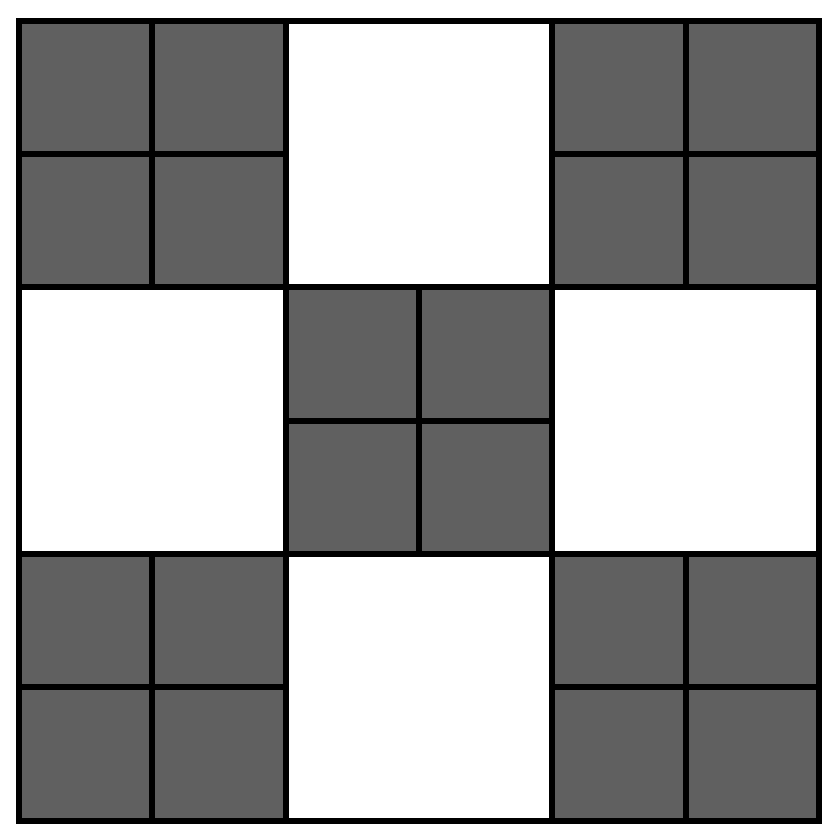
\includegraphics[width=0.3\textwidth]{./EPS/pointblockmatrix}\hfill
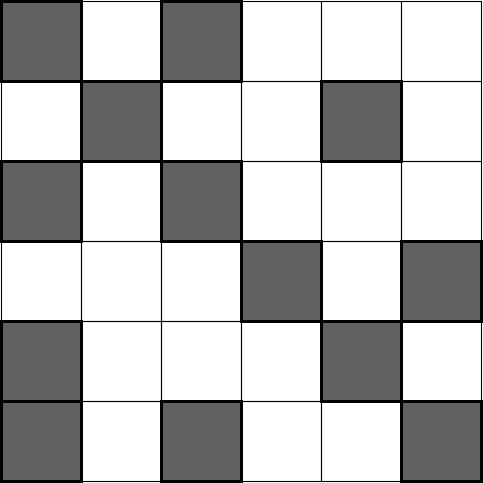
\includegraphics[width=0.3\textwidth]{./EPS/scalarmatrix}

\begin{minipage}{0.48\textwidth}
  \begin{itemize}
  \item  Point block matrix is a sparse matrix with small dense
blocks.
\item Realized by \lstinline!BCRSMatrix< FieldMatrix<E,2,2> >!. 
  \end{itemize}
\end{minipage}
\begin{minipage}{0.48\textwidth}
  \begin{itemize}
  \item Sparse matrix of scalars.
  \item Realized by \lstinline!BCRSMatrix< FieldMatrix<E,1,1> >!.
  \end{itemize}
\end{minipage}
\end{block}
\end{frame}


\subsubsection{The Backend}
\label{sec:backend}

\begin{frame}
  \frametitle{ISTL Vector Backend}
  \begin{itemize}
  \item \lstinline!template<int blocksize> class ISTLVectorBackend!
    is the currently available backend for ISTL vectors.
  \item The backend uses
    \lstinline!BlockVector<FieldVector<E,blocksize> >! as the
    underlying container.
  \item Attention: Make sure everything is correct for nonscalar backends
    \lstinline!blocksize!$>1$
  \end{itemize}
\end{frame}

\begin{frame}
  \frametitle{ISTL Matrix Backend}
  \begin{itemize} 
    \item \lstinline!template<int brows,int bcols> class ISTLBCRSMatrixBackend!
      is the currently available backend for ISTL sparse
      matrices.
    \item \lstinline!brows! is the number rows and \lstinline!bcols!
      is the number of columns of each matrix block.
  \item The backend uses
    \lstinline!BCRSMatrix<FieldMatrix<E,brows,bcols> >! as the
    underlying container.
  \item Attention: Make sure everything is correct for nonscalar backends
    \lstinline!blocksize!$>1$.
  \end{itemize}
\end{frame}
\begin{frame}[fragile]
  \frametitle{ISTL Sequential Solver Backends}
    \begin{itemize}
    \item \lstinline!ISTLBackend_SEQ_CG_SSOR!:  conjugate gradient method with SSOR preconditioner
    \item \lstinline!ISTLBackend_SEQ_BCGS_SSOR!: stabilized bi-conjugate gradient
      method with SSOR preconditioner
    \item \lstinline!ISTLBackend_SEQ_SuperLU!: SuperLU, a sparse
      direct solver
    \item \lstinline!template<class T> class ISTLBackend_SEQ_CG_AMG_SSOR! and
      \lstinline!template<class T> class ISTLBackend_SEQ_BICGS_AMG_SSOR! the
      above methods 
      preconditioned point-block AMG based on aggregation smoothed by SSOR.
    \end{itemize}
    Currently these sequential solvers are just a subset of the ones
  available in ISTL directly. More will follow in due time.
\end{frame}

\subsection{Parallel PDELab}
\label{sec:parallelization}

\begin{frame}
  \frametitle<presentatio>{Parallel PDELab}
  \begin{itemize}
  \item Go parallel by choosing
    \begin{enumerate}
    \item a suitable parallel grid (e.g. an overlapping one for
      overlapping domain decomposition methods),
    \item the correct constraints for the discretization of
      the PDE, and
    \item a suitable and matching parallel solver backend of the
      PDELab backend.
    \end{enumerate}
  \end{itemize}
\end{frame}

\begin{frame}
  \frametitle<presentation>{Parallel Solver Backends}
  
  There are three different kinds of parallel solvers classes
  available in the ISTL backend:
  \begin{itemize}
  \item Nonoverlapping domain decomposition
    methods.
  \item Overlapping domain decomposition metods.
  \item Data parallel solvers (e.g. AMG).
  \end{itemize}
\end{frame}

\begin{frame}
  \frametitle{Building Blocks for Parallel Solvers}

  \begin{itemize}
  \item The solvers in ISTL do not use matrix and vector structures
    directly,
  \item but implementations of \lstinline!Preconditioner!,
    \lstinline!LinearOperator! and \lstinline!ScalarProduct!.
  \item These components must match in the solver category
    (e.g. sequential, overlapping, nonoverlapping) and thus support
    the same data decomposition.
  \item Simply plugin parallel instances of the components to get
    parallel solvers.
  \end{itemize}
\end{frame}

\begin{frame}
  \frametitle<presentation>{Building Blocks for Parallel Solvers}
  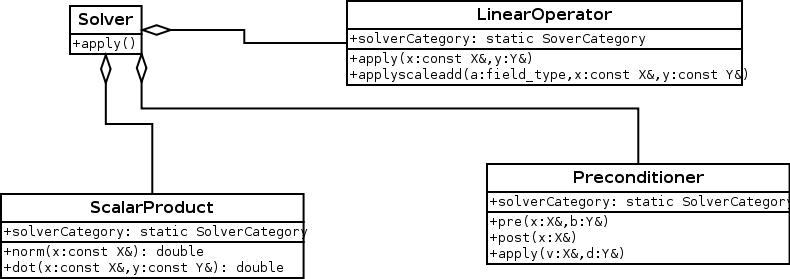
\includegraphics[width=\textwidth]{EPS/istlsolver}
\end{frame}

\begin{frame}
  \frametitle{Some Parallel Solver Backends}
  The solver backends can be found in header
  dune/pdelab/backend/istlsolverbackend.hh. Template parameter GFS is
  the type of the grid function space, template parameter C the type
  of the parallel constraints used.
  \begin{itemize}
  \item \lstinline!template<class GFS> class ISTLBackend_NOVLP_BCGS_NOPREC!:
    parallel unpreconditioned
    stabilized bi-conjugate gradient method for nonoverlapping grids.
    \item \lstinline!template<class GFS> class ISTLBackend_OVLP_BCGS_SSORk!:
      the above preconditioned with $k$ steps of SSOR.
    \item \lstinline!template<class GFS, class C> class ISTLBackend_OVLP_BCGS_SuperLU!:
      the first method preconditioned by an overlapping domain
      decomposition method with SuperLU for the problems local to the
      processors.
      \item \lstinline!template<class GFS> ISTLBackend_BCGS_AMG_SSOR!:
        the first method preconsitioned by parallel AMG smoothed by
        SSOR. Requires an overlapping grid!
  \end{itemize}
\end{frame}

\begin{frame}[fragile]
  \frametitle{Nonoverlapping example}
  \begin{lstlisting}[basicstyle=\tiny]
// 1. Create an non-overlapping grid
Dune::FieldVector<double,2> L(1.0);
Dune::FieldVector<int,2> N(16);
Dune::FieldVector<bool,2> periodic(false);
int overlap=0; // needs overlap 0 because overlap elements are not assembled
Dune::YaspGrid<2> grid(helper.getCommunicator(),L,N,periodic,overlap);
typedef Dune::YaspGrid<2>::LeafGridView GV;
const GV& gv=grid.leafView();

// 2. Create correctly constrained grid function space
typedef Dune::PDELab::Q1LocalFiniteElementMap<Coord,Real,dim> FEM;
FEM fem;
typedef Dune::PDELab::NonoverlappingConformingDirichletConstraints CON;
CON con;
typedef Dune::PDELab::ISTLVectorBackend<1> VBE;
typedef Dune::PDELab::GridFunctionSpace<GV,FEM,CON,VBE,
Dune::PDELab::SimpleGridFunctionStaticSize> GFS;
GFS gfs(gv,fem,con);
con.compute_ghosts(gfs); // con stores indices of ghost dofs
typedef ConvectionDiffusionProblem<GV,Real> Param;
Param param;
typedef Dune::PDELab::BoundaryConditionType_CD<Param> B;
B b(gv,param);
typedef Dune::PDELab::DirichletBoundaryCondition_CD<Param> G;
G g(gv,param);
\end{lstlisting}
\end{frame}
\begin{frame}[fragile]
\frametitle<presentation>{Nonoverlapping Example Continued}
  \begin{lstlisting}[basicstyle=\tiny]
// Compute constrained space
typedef typename GFS::template ConstraintsContainer<Real>::Type C;
C cg;
Dune::PDELab::constraints(b,gfs,cg);

// Compute affine shift
typedef typename GFS::template VectorContainer<Real>::Type V;
V x(gfs,0.0);
Dune::PDELab::interpolate(g,gfs,x);
Dune::PDELab::set_nonconstrained_dofs(cg,0.0,x);

// Make grid operator space
typedef Dune::PDELab::ConvectionDiffusion<Param> LOP; 
LOP lop(param,2);
typedef Dune::PDELab::ISTLBCRSMatrixBackend<1,1> MBE;
typedef Dune::PDELab::GridOperatorSpace<GFS,GFS,LOP,C,C,MBE,true> GOS;
GOS gos(gfs,cg,gfs,cg,lop);

// 3. Choose a linear solver 
typedef Dune::PDELab::ISTLBackend_NOVLP_BCGS_NOPREC<GFS> LS;
LS ls(gfs,5000,1);
...
\end{lstlisting}
  
\end{frame}

\begin{frame}[fragile]
  \frametitle{Overlapping Example}
  \begin{lstlisting}[basicstyle=\tiny]
// 1. Create an overlapping grid
Dune::FieldVector<double,2> L(1.0);
Dune::FieldVector<int,2> N(16);
Dune::FieldVector<bool,2> periodic(false);
int overlap=2; 
Dune::YaspGrid<2> grid(helper.getCommunicator(),L,N,periodic,overlap);
typedef Dune::YaspGrid<2>::LeafGridView GV;
const GV& gv=grid.leafView();

// 2. Create correctly constrained grid function space
typedef Dune::PDELab::Q1LocalFiniteElementMap<Coord,Real,dim> FEM;
FEM fem;
typedef Dune::PDELab::OverlappingConformingDirichletConstraints CON;
typedef Dune::PDELab::ISTLVectorBackend<1> VBE;
typedef Dune::PDELab::GridFunctionSpace<GV,FEM,CON,VBE,
Dune::PDELab::SimpleGridFunctionStaticSize> GFS;
GFS gfs(gv,fem);

//  define problem parameters
typedef ConvectionDiffusionProblem<GV,Real> Param;
Param param;
typedef Dune::PDELab::BoundaryConditionType_CD<Param> B;
B b(gv,param);
typedef Dune::PDELab::DirichletBoundaryCondition_CD<Param> G;
G g(gv,param);
\end{lstlisting}  
\end{frame}
\begin{frame}[fragile]
\frametitle<presentation>{Overlapping Example Continued}
  \begin{lstlisting}[basicstyle=\tiny]

//  Compute constrained space
typedef typename GFS::template ConstraintsContainer<Real>::Type C;
C cg;
Dune::PDELab::constraints(b,gfs,cg);
//  Compute affine shift
typedef typename GFS::template VectorContainer<Real>::Type V;
V x(gfs,0.0);
Dune::PDELab::interpolate(g,gfs,x);
Dune::PDELab::set_nonconstrained_dofs(cg,0.0,x);
// Make grid operator space
typedef Dune::PDELab::ConvectionDiffusion<Param> LOP; 
LOP lop(param,2);
typedef Dune::PDELab::ISTLBCRSMatrixBackend<1,1> MBE;
typedef Dune::PDELab::GridOperatorSpace<GFS,GFS,LOP,C,C,MBE> GOS;
GOS gos(gfs,cg,gfs,cg,lop);

// 3. Choose a linear solver 
typedef Dune::PDELab::ISTLBackend_OVLP_BCGS_SuperLU<GFS,C> LS;
LS ls(gfs,cg,5000,2);
...
\end{lstlisting}
  
\end{frame}
}
%%% Local Variables: 
%%% mode: latex
%%% TeX-master: 
%%% End: 
}
\mode<all>{%\only<presentation>{

%\lstset{language=C++, basicstyle=\ttfamily, 
%  keywordstyle=\color{red}\bfseries, tabsize=4, stringstyle=\ttfamily,
%  commentstyle=\it, extendedchars=true, escapeinside={/*@}{@*/}}

%\lstset{language=C++, basicstyle=\scriptsize\ttfamily,
%  stringstyle=\ttfamily, commentstyle=\it, extendedchars=true,
%  numbers=left, numberstyle=\tiny, stepnumber=2, numbersep=5pt,
%  breakatwhitespace=true, breaklines=true}
%\definecolor{darkgray}{gray}{0.4}
%\lstset{keywordstyle=\color{violet},
%        commentstyle=\color{darkgray},
%        stringstyle=\color{orange},
%        emph={bool,int,unsigned,char,true,false,void}, emphstyle=\color{blue},
%        emph={[2]\#include,\#define,\#ifdef,\#endif}, emphstyle={[2]\color{violet}},
%        }
%}
%\only<article>{
%\lstset{language=C++, basicstyle=\small, 
%  keywordstyle=\bfseries, tabsize=4, stringstyle=\ttfamily,
%  commentstyle=\it, extendedchars=true, escapeinside={/*@}{@*/}}

%\lstset{language=C++, basicstyle=\small\ttfamily,
%  stringstyle=\ttfamily, commentstyle=\it, extendedchars=true,
%  numbers=left, numberstyle=\tiny, stepnumber=2, numbersep=5pt,
%  breakatwhitespace=true, breaklines=true}
%\definecolor{darkgray}{gray}{0.4}
%\lstset{keywordstyle=\color{violet},
%        commentstyle=\color{darkgray},
%        stringstyle=\color{orange},
%        emph={bool,int,unsigned,char,true,false,void}, emphstyle=\color{blue},
%        emph={[2]\#include,\#define,\#ifdef,\#endif}, emphstyle={[2]\color{violet}},
%        }
%        }

\section{Parallel PDELab}
\subsection{Introduction}

\subsubsection{Why Parallel Computing?}

\begin{frame}
\frametitle<presentation>{Why Parallel Computing?}

\begin{itemize}
\item The speed of individual computer cores is not increasing 
essentially since some years
\item The number of cores is increasing. Dual-cores are the rule, 
up to 12-core processors are available.
\item Several multi-core processors can be used on one mainboard (e.g. four 12-core processors)
\item Computer cluster with several multi-core multi-processor servers are affordable even for small companies
\item High-performance computer have up to 294912 cores (JUGENE).
\end{itemize}

\end{frame}

%-----------------------------------------------------------------------------

\subsubsection{Architectures of Parallel Computers}

\begin{frame}
\frametitle<presentation>{Architectures of Parallel Computers}
\begin{itemize}
\item Shared-memory computing: all cores have access to the whole memory
\begin{itemize}
\item Uniform memory access architecture (UMA): access to every memory location from every processor takes the
same amount of time (multi-core CPUs)
\item Non-uniform memory access architecture (NUMA): memory is associated with processors but address space is 
global. Local memory can be accessed faster than memory attached
to other processors (multi-processor servers)
\end{itemize}
\item Message passing architecture (MP): each processor can only access local memory, information is exchanged
between processors with messages send over a network (computer clusters, super computer)
\end{itemize}
\end{frame}


\begin{frame}
\frametitle{Comparison of Architectures by Example}
\begin{itemize}
\item Given vectors $x,y\in\mathbb{R}^N$, compute scalar product $s =
  \sum_{i=0}^{N-1} x_i y_i$:
\begin{itemize}
\item[(1)] Subdivide index set into $P$ pieces. 
\item[(2)] Compute $s_p=\sum_{i=pN/P}^{(p+1)N/P-1} x_i y_i$ in
  parallel.
\item[(3)] Compute $s = \sum_{i=0}^{P-1} s_i$.
\end{itemize}
\item \textit{Uniform memory access architecture}: Store vectors as in
  sequential program:
\begin{center}
  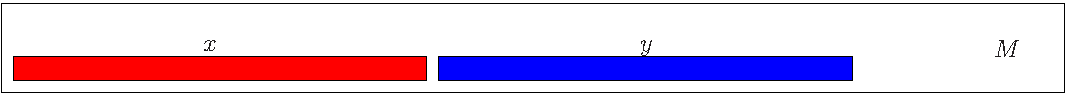
\includegraphics[width=0.9\textwidth]{EPS/umalayout}
\end{center}
\item \textit{Nonuniform memory access architecture}: Distribute
  data to the local memories:
\begin{center}
  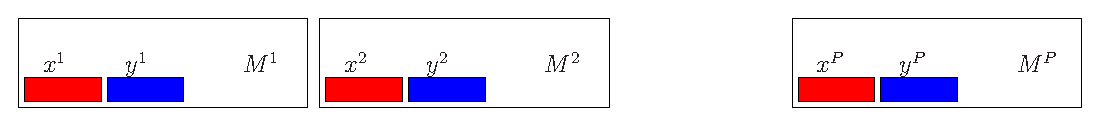
\includegraphics[width=0.9\textwidth]{EPS/numalayout}
\end{center}
\item \textit{Private memory architecture}: Same as for NUMA! 
\item Distributing data structures is hard and not automatic in
  general.
\item Parallelisation effort for NUMA and MP is almost the same.
\end{itemize}
\end{frame}


\subsubsection{Message Passing}
\begin{frame}
\frametitle<presentation>{Message Passing}

\begin{itemize}
\item Users view: Copy (contiguous) memory block from one address space to the
  other.
\item Message is subdivided into individual packets.
\item Network is packet-switched. 
\item A packet consists of an envelope and
  the data:
\begin{center}
  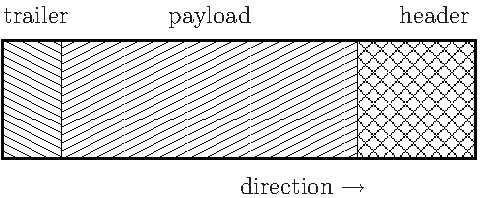
\includegraphics[width=0.49\textwidth]{EPS/paket}
\end{center}
\item Header: Destination, size and kind of data.
\item Payload: Size ranges from some bytes to kilobytes.
\item Trailer: E.g. checksum for error detection.
\end{itemize}
\end{frame}

%----------------------------------------------------------------------------------------
\begin{frame}
\frametitle{The Message Passing Interface (MPI)}

\begin{itemize}
\item Portable Library with functions for message exchange between processes
\item Developed 1993-94 by a international board
\item Available on nearly all computer platforms
\item Free Implementations also for LINUX Clusters: {\bf MPICH}\footnote{\href{http://www-unix.mcs.anl.gov/mpi/mpich}{{\tiny http://www-unix.mcs.anl.gov/mpi/mpich}}}
 and {\bf OpenMPI}\footnote{\href{http://www.open-mpi.org/}{{\tiny http://www.open-mpi.org/}}} (former {\bf LAM})
\item Properties of MPI:
\begin{itemize}
\item library with C-, C++ and Fortran bindings (no language extension)
\item large variety of point-to-point communication functions
\item global communication
\item data conversion for heterogeneous systems
\item subset formation and topologies possible
\end{itemize}

\end{itemize}

\begin{small}\textit{Remark:} There is a special MPICH version for shared-memory machines using memory copy operations instead of slower mesage passing algorithms.
OpenMPI can even distinguish between processes which share the same address space and
processes on remote machines and use either memory copy or message passing.
\end{small}
\end{frame}

\subsubsection{Strong Scalability Example}
\begin{frame}
\frametitle<presentation>{Strong Scalability of 3D Parallel Computation}
\begin{center}
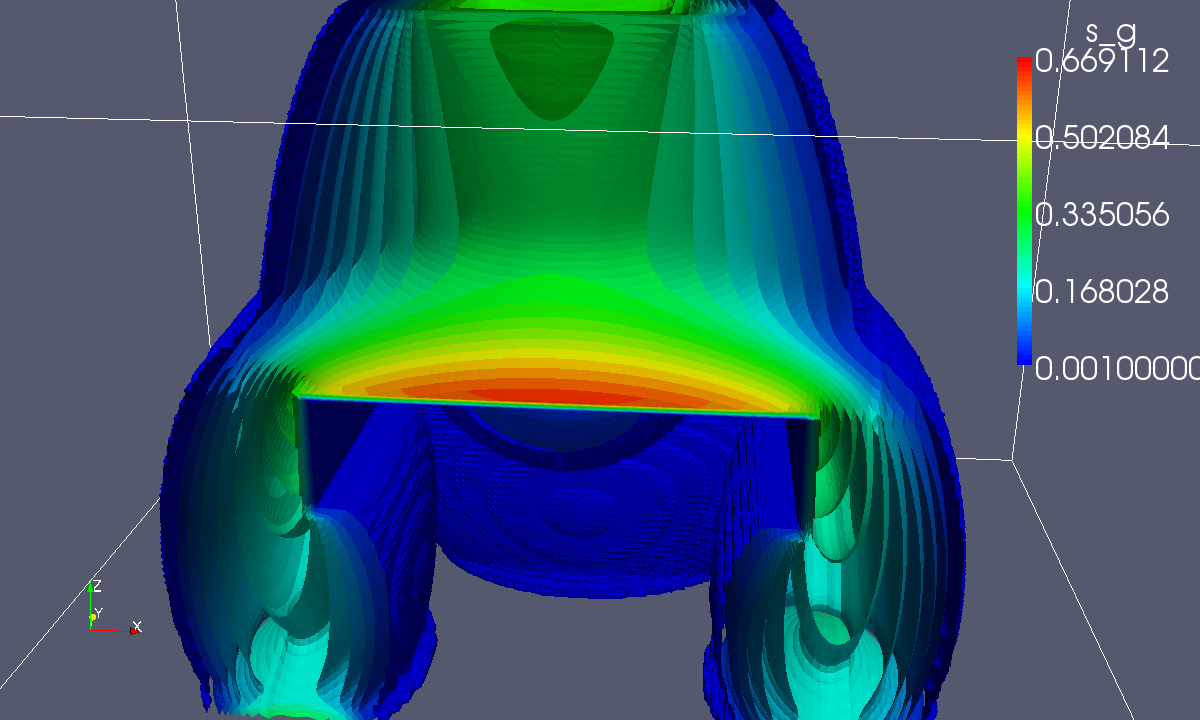
\includegraphics[width=0.9\textwidth]{EPS/dnapl-3d-het-iso}\\
3D DNAPL Infiltration
\end{center}
\end{frame}


\begin{frame}
\frametitle<presentation>{Strong Scalability of 3D Parallel Computation}
Simulation of a DNAPL infiltration with a coarse lense on a grid with  $160 \times 160 \times 96$
unknowns on a server with 4$\times$12  AMD Magny Cours, 2.1 GHz, 12$\times$0.5MB L2, 12MB
L3 processors.

Computation time for one time step with BiCGStab + AMG preconditioner:

\begin{center}
\begin{tabular}{r|rrr|rr|rr}
\hline
P  & \#IT(max) & $T_{it}$ & S & $T_{asm}$ & S & $T_{total}$ & S \\
\hline
 1  &  6.5 & 4.60 &      - &  43.7 &      - & 713.8 &    - \\
 4  &  10  & 1.85 &   2.5 &  17.5 &   2.5 & 295.9 & 2.4 \\
 8  &  9    & 0.63 &   7.3 &    8.4 &   5.2 & 127.1 & 5.6 \\
16 &  9.5 & 0.40 & 11.5 &    4.1 & 10.7 &   73.1 & 9.8 \\
32 &  15  & 0.27 & 17.0 &    1.9 & 23.0 &   43.5 & 16.4 \\ 
\hline
\end{tabular}
\end{center} 

Comparison with T3E from 1999

\begin{center}
\begin{tabular}{r|rrrr}
\hline
Machine  & Cells & Time steps & Newton steps & $T_{total}$ \\
\hline
256 T3E        & 2621440 &  50 & 264 & 14719\\
16 Cores AMD & 2457600 & 50 & 231 & 2500\\ 
\hline
\end{tabular}
\end{center} 
\end{frame}


\subsection{Domain Decomposition}
\begin{frame}
  \frametitle<presentation>{Domain Decomposition}

  \begin{itemize}
  \item partition a problem by splitting the domain it into small subdomains
  \item each part is solved by a different processor
  \item goes back to an idea of H.A. Schwarz who in 1890 presented a method to prove the existence of
        solutions of the Laplace equation on ``complicated'' domains.
  \item Different variants:
    \begin{itemize}
    \item overlapping domain decomposition
    \item non-overlapping domain decomposition
    \end{itemize}
  \end{itemize}
  
  \begin{center}
    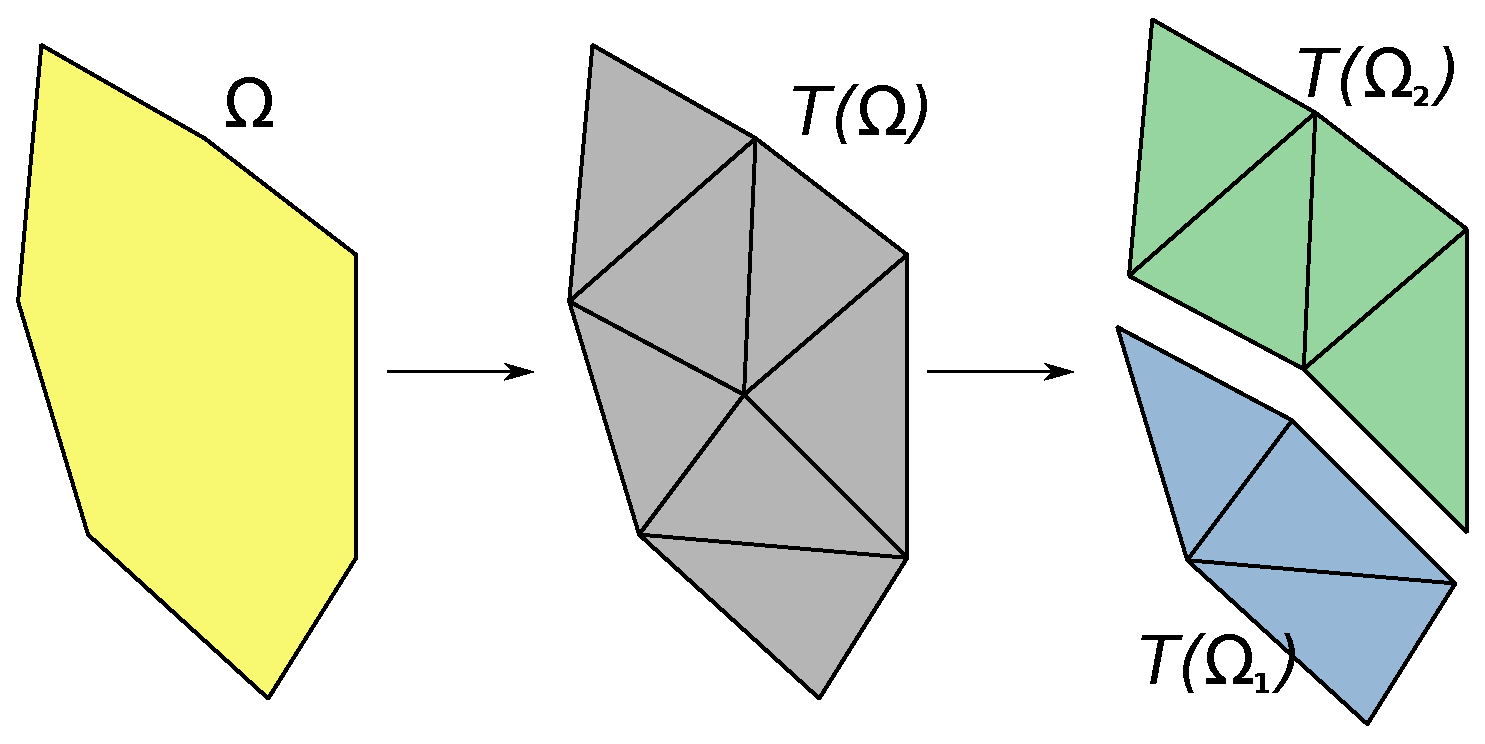
\includegraphics[width=.6\linewidth]{EPS/dd}
  \end{center}

\end{frame}

\subsubsection{Nonoverlapping Domain Decomposition}
\begin{frame}
  \frametitle<presentation>{Nonoverlapping Domain Decomposition}

  \begin{columns}
    \begin{column}{0.6\linewidth}
      % In overlapping domain decomposition methods, the subdomains
      % overlap by more than the interface. Overlapping domain
      % decomposition methods
      % include the Schwarz alternating method and the additive
      % Schwarz
      % method. Many domain decomposition methods can be written and
      % analyzed as a special case of the abstract additive Schwarz
      % method.
    
      \begin{itemize}
      \item Given a domain $\Omega\subseteq\mathbb{R}^d$
        % and a triangulation $T(\Omega) = \{E\}$
        % \item partition the cells $E$ such that there is exactly one
        %   processor with $E \in T(\Omega_i)$
      \item partition $\Omega$ into \emph{non-overlapping}
        sub-domains:
        \[
        \Omega_i\colon\quad \bigcup_{i=1}^p \overline{\Omega_i} = \overline{\Omega}, \quad
        \Omega_i\cap\Omega_j=\emptyset \;\forall i\ne j.
        \]
      \end{itemize}
    \end{column}
    \begin{column}{0.4\linewidth}
      \begin{onlyenv}<presentation>
        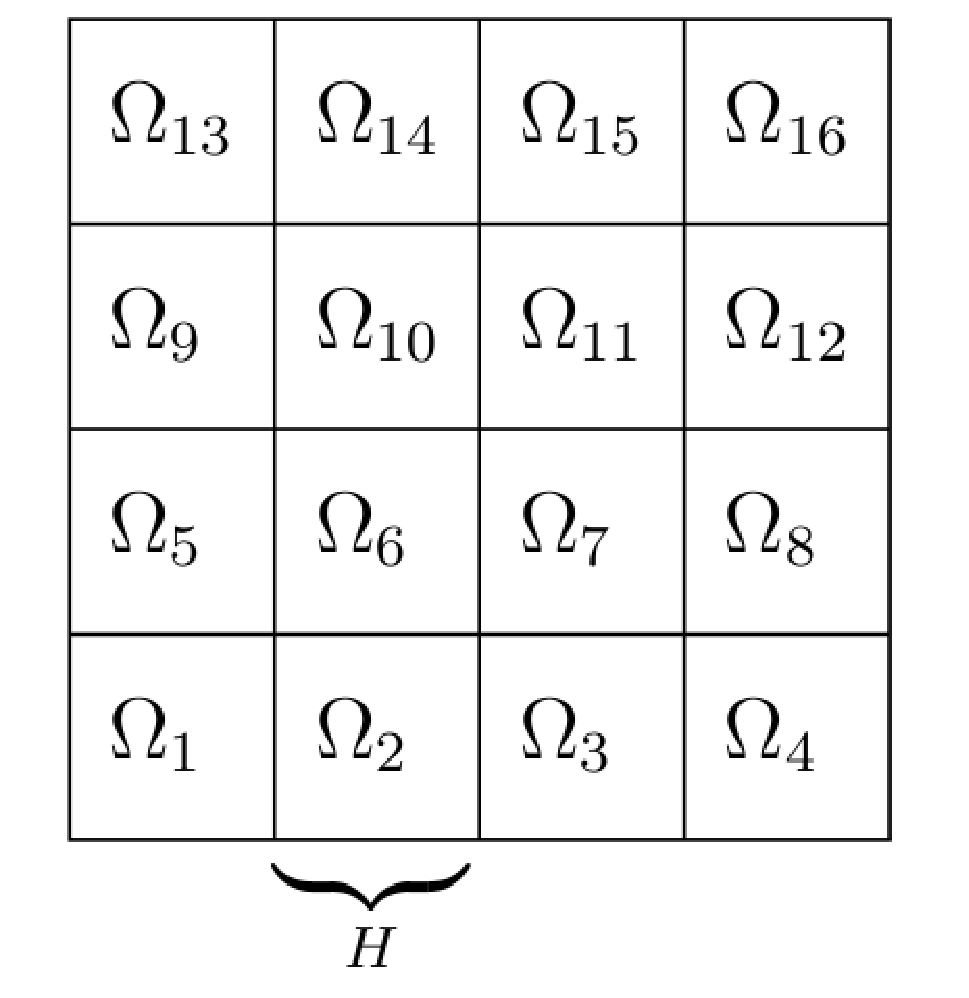
\includegraphics[width=0.6\linewidth]{EPS/konstr_n_uberl_str}
        \vskip5mm
        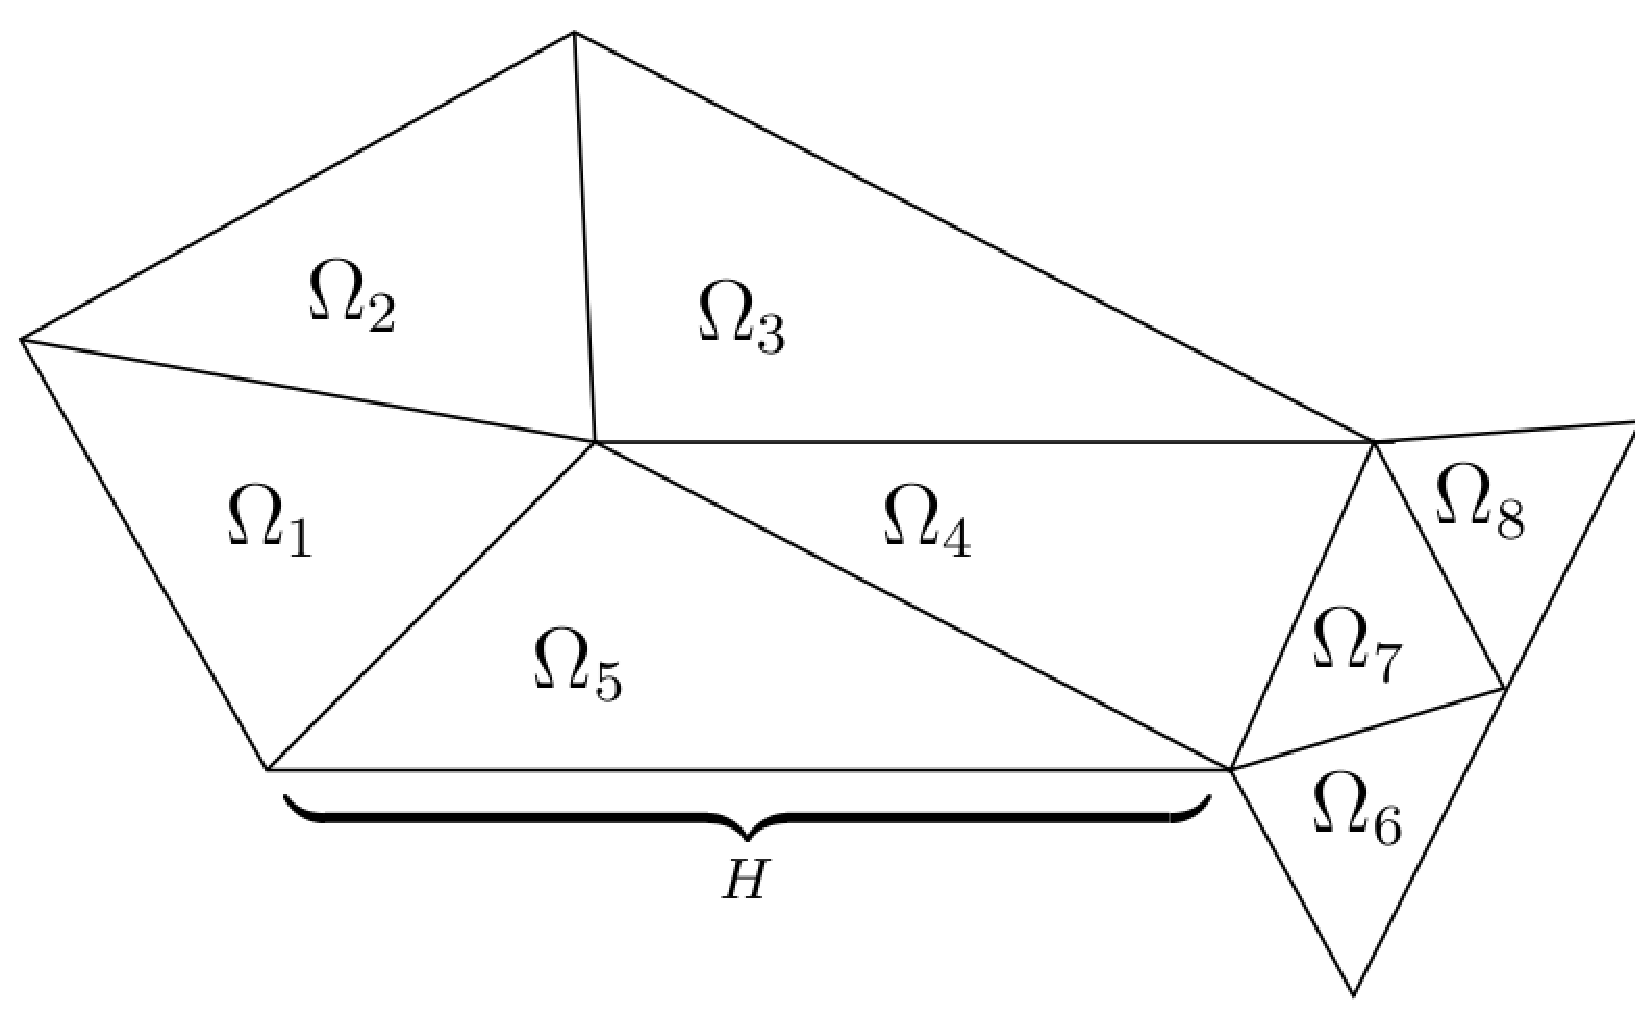
\includegraphics[width=0.9\linewidth]{EPS/konstr_n_uberl_unstr}
      \end{onlyenv}
      \begin{onlyenv}<article>
        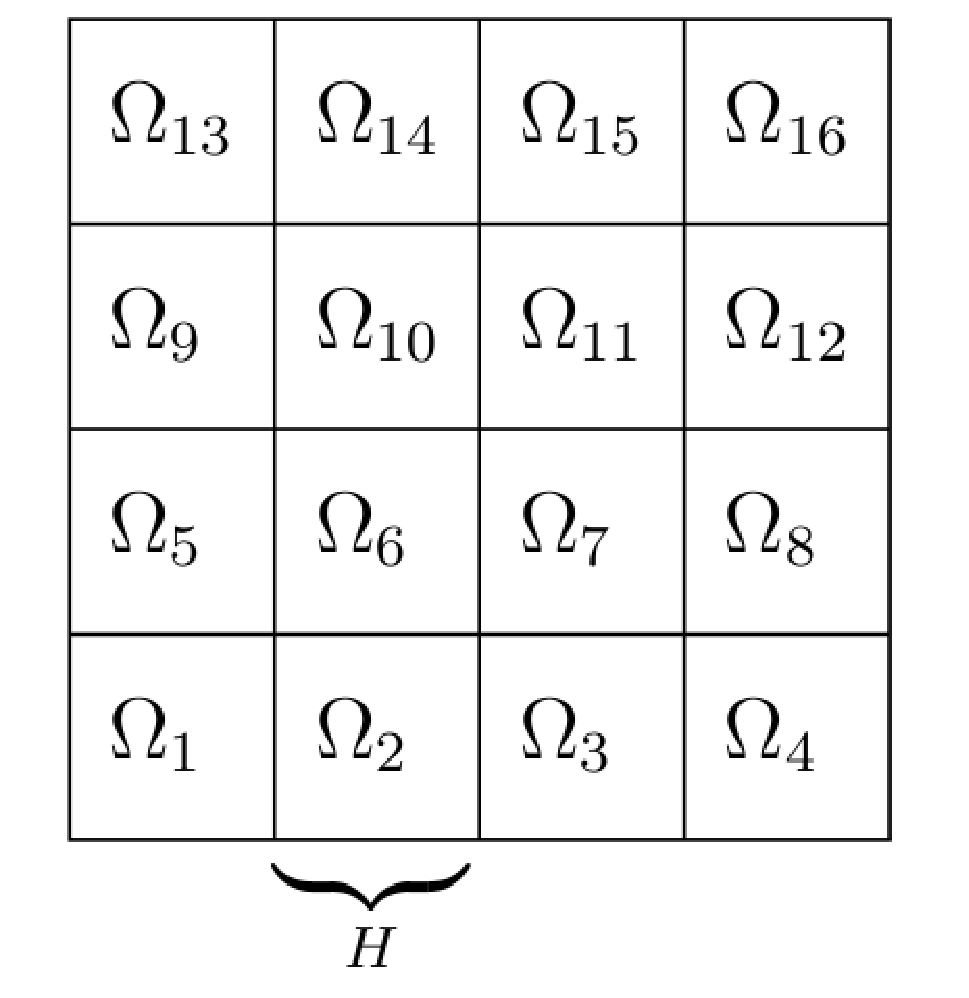
\includegraphics[width=0.25\linewidth]{EPS/konstr_n_uberl_str}
        \vskip5mm
        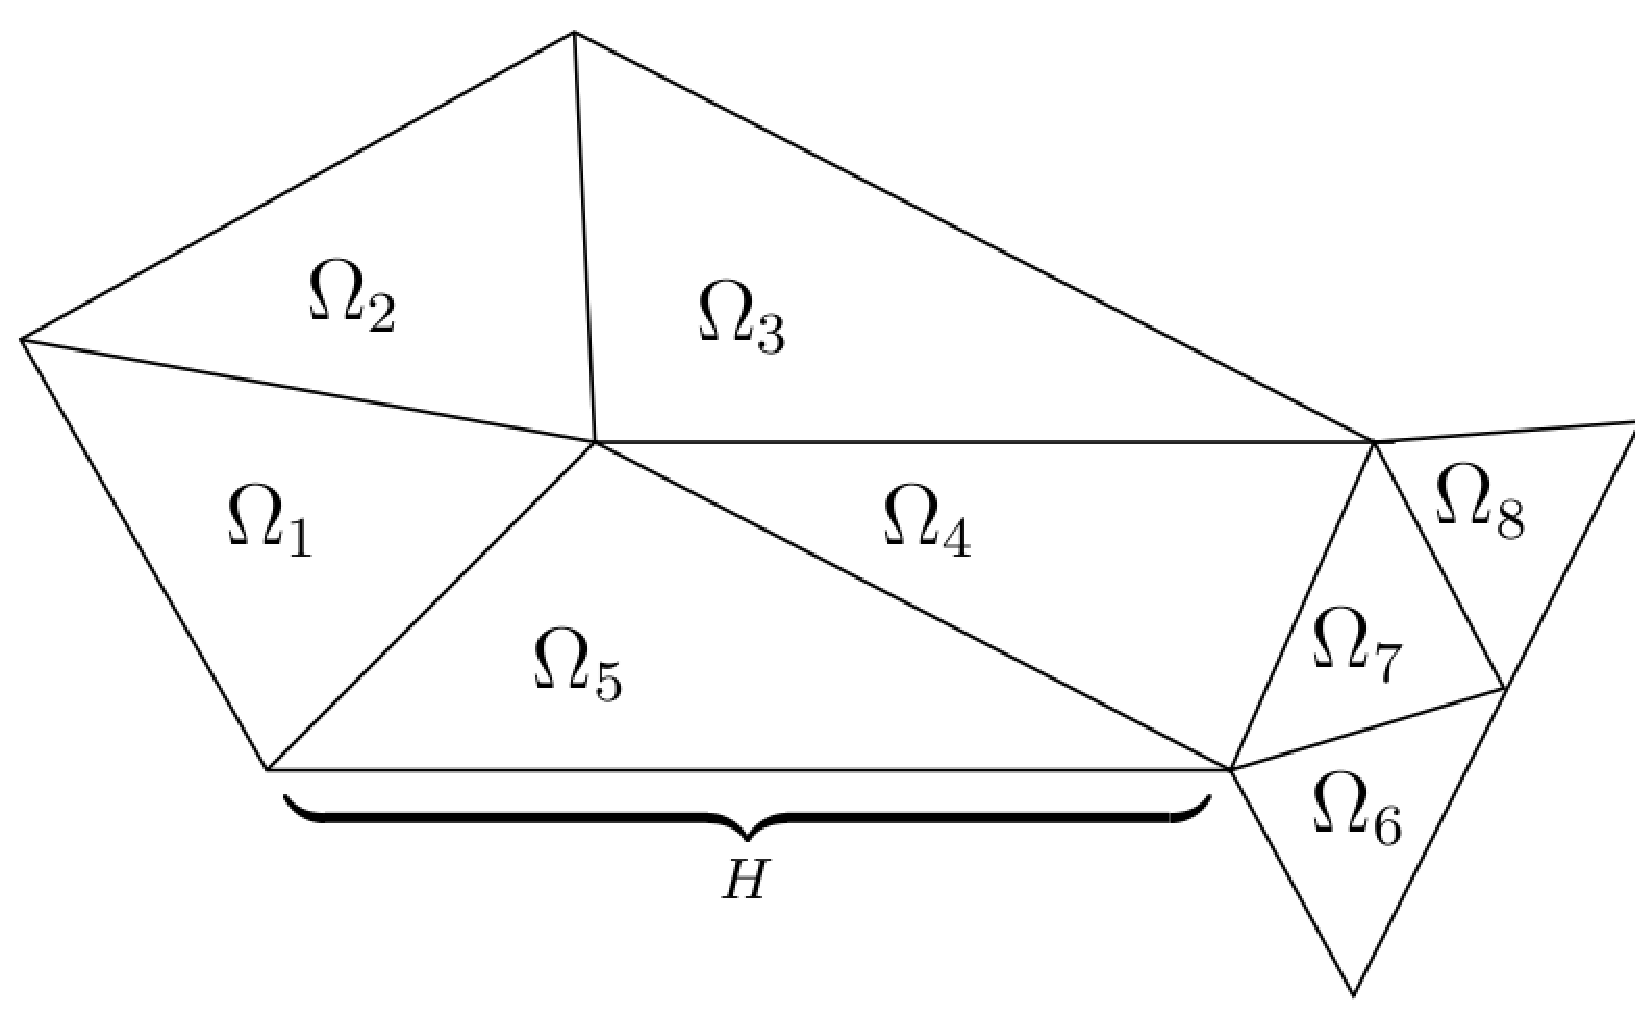
\includegraphics[width=0.36\linewidth]{EPS/konstr_n_uberl_unstr}
      \end{onlyenv}
    \end{column}
  \end{columns}
\end{frame}

\subsubsection{Overlapping Domain Decomposition}
\begin{frame}
  \frametitle<presentation>{Overlapping Domain Decomposition}

  \begin{columns}
    \begin{column}{0.6\linewidth}
      % In overlapping domain decomposition methods, the subdomains
      % overlap by more than the interface. Overlapping domain
      % decomposition methods
      % include the Schwarz alternating method and the additive
      % Schwarz
      % method. Many domain decomposition methods can be written and
      % analyzed as a special case of the abstract additive Schwarz
      % method.
    
      \begin{itemize}
      \item Extend each $\Omega_i$ by an overlap $\hat \Omega_i$ of width
        $\beta\cdot H$:
        \[
        \hat \Omega_i = \left\{ x\in\Omega \mid \mathsf{dist}(x,\Omega_i) < \beta\cdot H \right\}
        \]
      \end{itemize}
    \end{column}
    \begin{column}{0.4\linewidth}
      \begin{onlyenv}<presentation>
        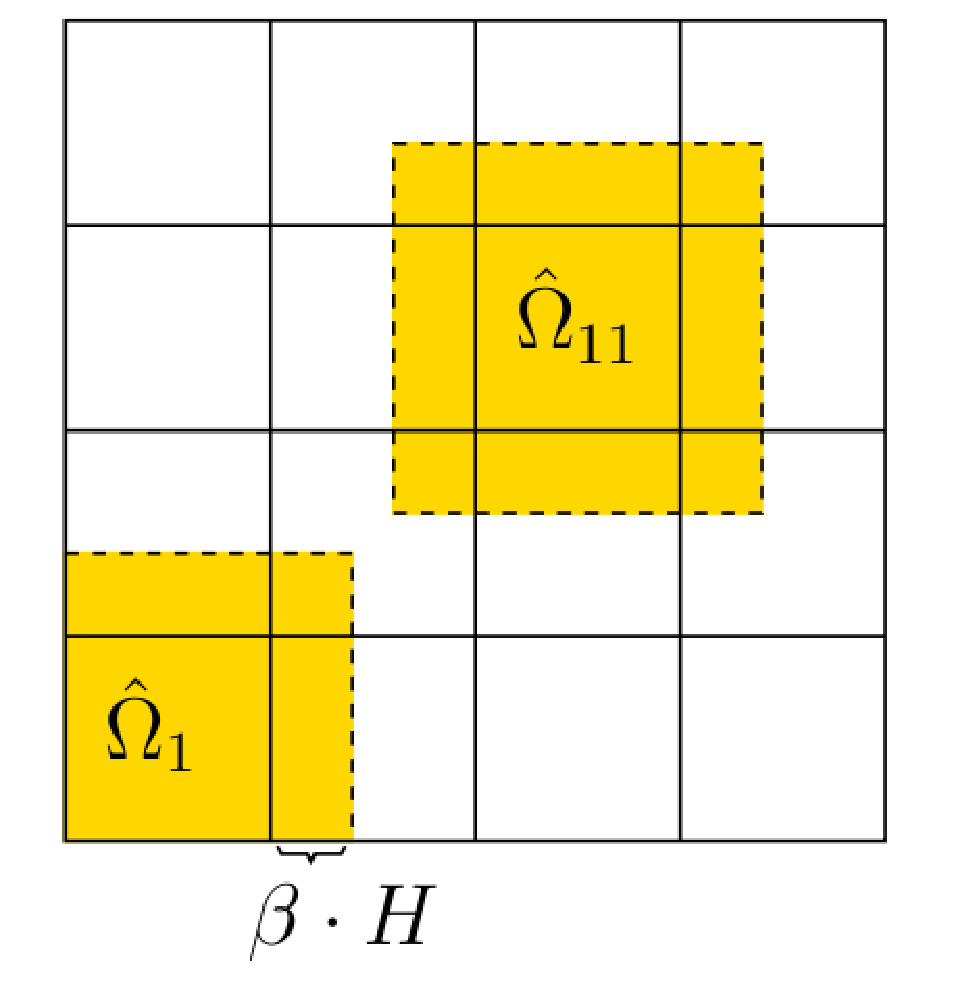
\includegraphics[width=0.6\linewidth]{EPS/konstr_uberl_str}
        \vskip5mm
        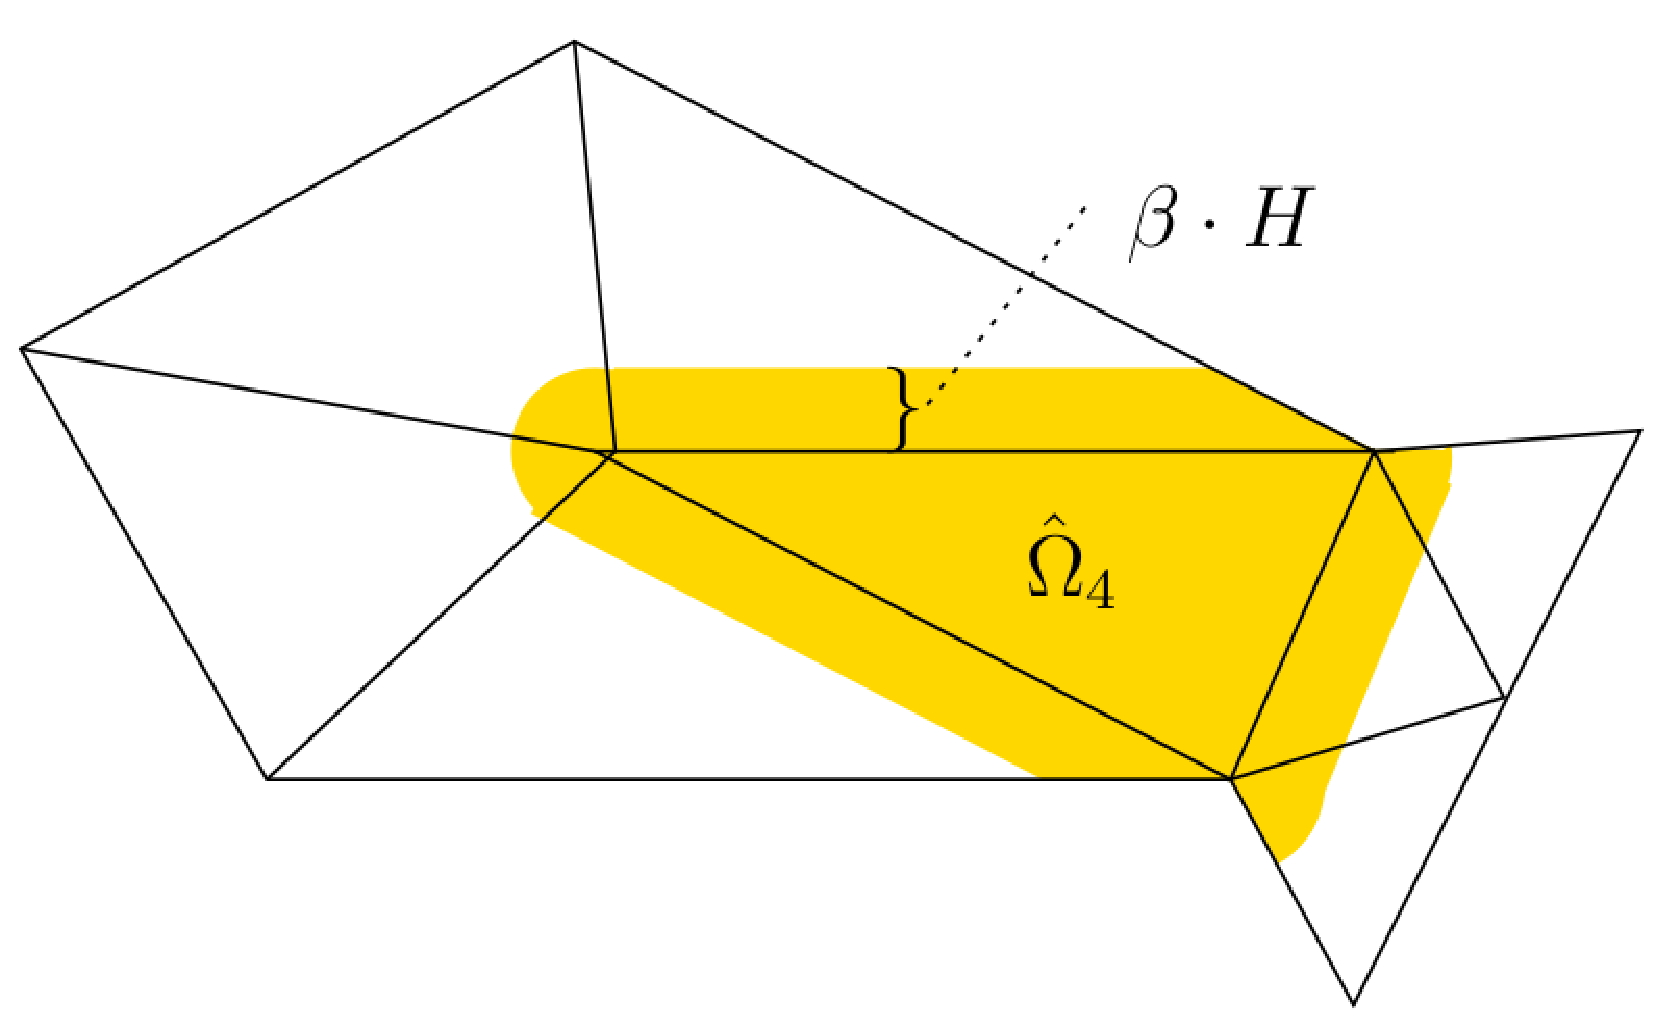
\includegraphics[width=0.9\linewidth]{EPS/konstr_uberl_unstr}
      \end{onlyenv}
      \begin{onlyenv}<article>
        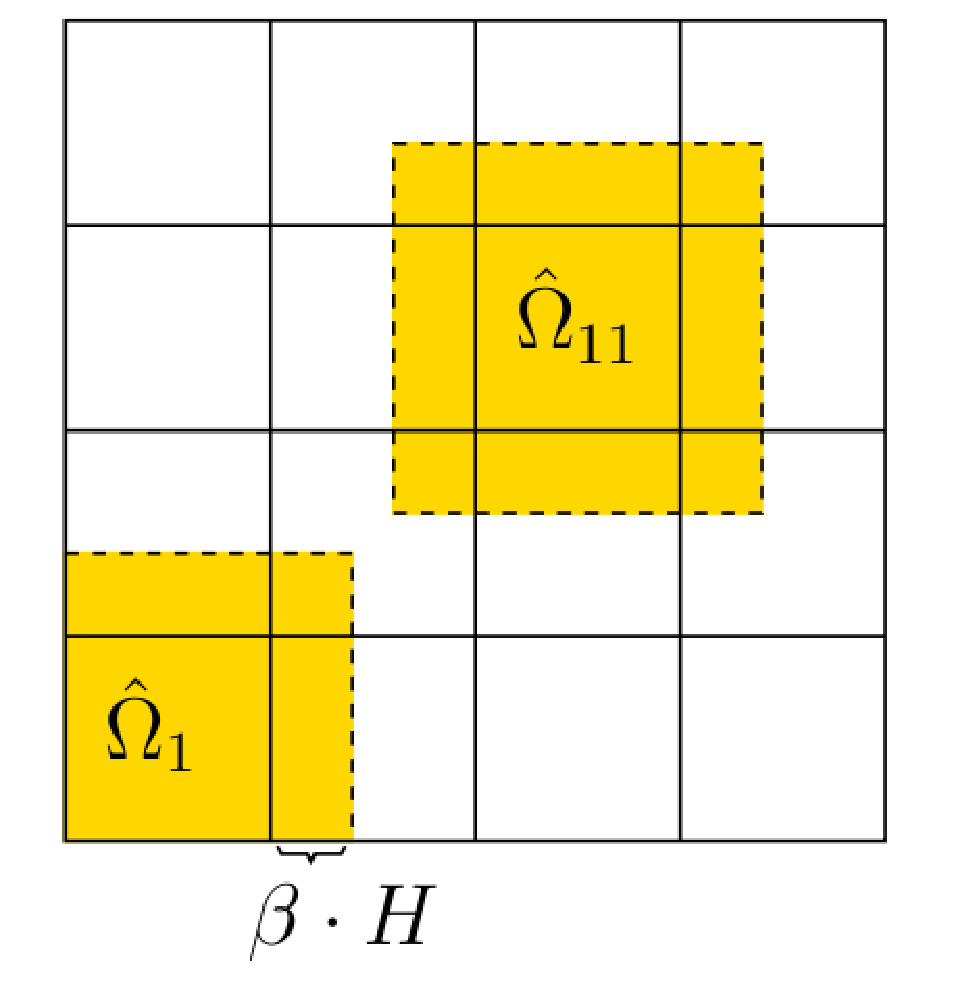
\includegraphics[width=.25\linewidth]{EPS/konstr_uberl_str}
        \vskip5mm
        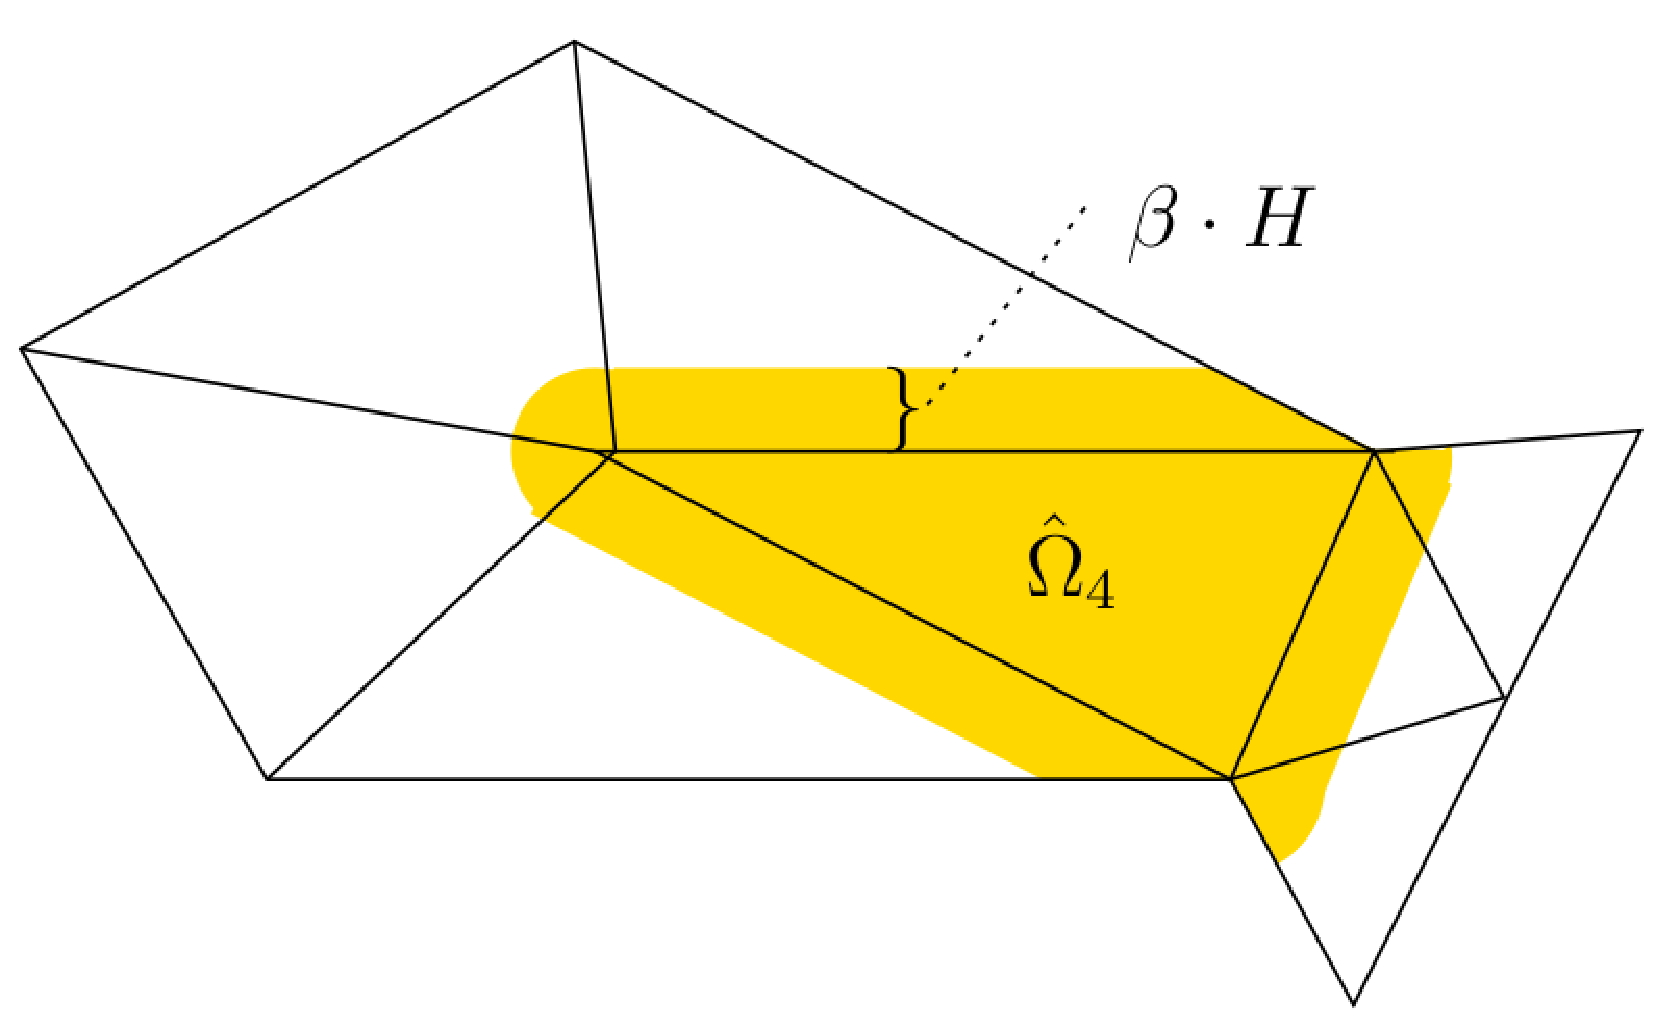
\includegraphics[width=.36\linewidth]{EPS/konstr_uberl_unstr}
      \end{onlyenv}
    \end{column}
  \end{columns}
\end{frame}

\subsection{Parallel Grids}
%-----------------------------------------------------------------------------

\subsubsection{Partition Types}
\begin{frame}[fragile]
\frametitle<presentation>{Partition Types}

\begin{itemize}
\item Each grid entity can be present on one or more processors.
\item Each entity on one processor has a partition type, which can be determined 
by the method\\
        \hspace*{1cm}\lstinline!entity.partitionType()!
\item The possible partition types are:\\
\end{itemize}
\begin{tabular}{ll}
  \em \bfseries interior 
  & Entity is owned by the process\\
  \em \bfseries overlap & Entity is owned by a different process, but a full copy exists\\
  \em \bfseries ghost
  & Entity is owned by a different process, but a partial copy\\
  & exists\\
  \em \bfseries border
  & Boundary of interior. (only exists for entities with \\
  & codimension$>$0)\\
  \em \bfseries front
  & Boundary of interior+overlap if not {\em \bfseries border} (only exists for\\
  & entities with codimension$>$0)
\end{tabular}
\end{frame}


\begin{frame}[fragile]
\frametitle{Partition Types Example}
\begin{columns}[c]
\begin{column}{0.7\textwidth}

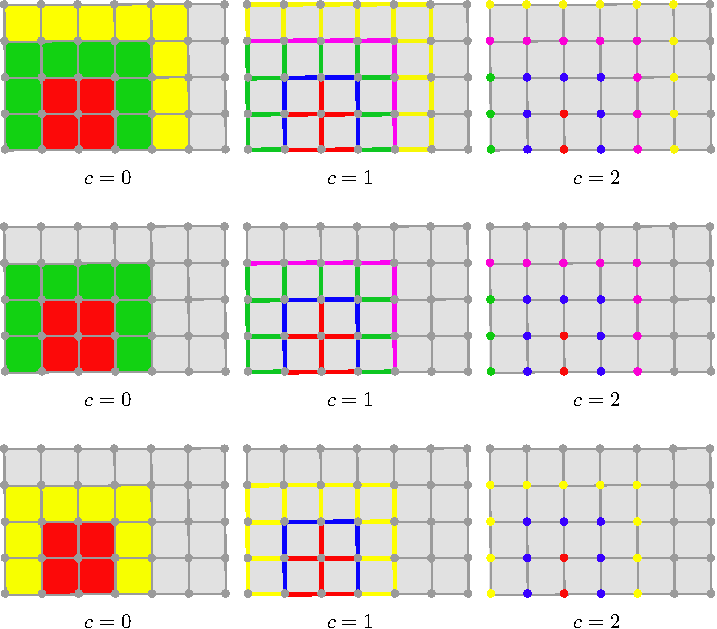
\includegraphics[width=\textwidth]{EPS/partitionsingle}
\end{column}
\begin{column}{0.3\textwidth}
\vskip0.5cm
\textbf{First row}: with overlap and ghosts\\
\textbf{Second row}: with overlap only\\
\textbf{Third row}: with ghosts only
\vskip5mm
\begin{center}
\begin{tabular}{|c|}
\hline\color{red} interior\\\hline
\color{green} overlap\\\hline
\color{yellow} ghost\\\hline
\color{blue} border\\\hline
\color{magenta} front\\\hline
\color{gray} not stored\\\hline
\end{tabular}
\end{center}
\end{column}
\end{columns}

\end{frame}

\subsubsection{Parallel Grids in Dune}

\begin{frame}
  \frametitle<presentation>{Parallel Grids in Dune}
  \begin{itemize}
  \item<1-> \lstinline[basicstyle=\normalfont\ttfamily]!YaspGrid!
      \begin{itemize}
      \item structured
      \item 2D/3D
      \item arbitrary overlap
      \end{itemize}
  \item<2-> \lstinline[basicstyle=\normalfont\ttfamily]!UGGrid!
      \begin{itemize}
      \item unstructured
      \item 2D/3D
      \item multi-element
      \item one layer of ghost cells
      \item (conforming) red-green refinement
      \item (non-free!)
      \end{itemize}
  \item<3-> \lstinline[basicstyle=\normalfont\ttfamily]!ALUGrid!
      \begin{itemize}
      \item unstructured
      \item 3D
      \item tetrahedral or hexahedral elements
      \item ghost cells
      \item (non-conforming) bisection refinement
      \end{itemize}
  \end{itemize}
\end{frame}

\subsubsection{Iterators in a parallel Grid}

\begin{frame}[fragile]
  \frametitle<presentation>{Iterators in a parallel Grid}
  \small
  Dune offers Iterators which only iterate over elements with certain partition types:\\
\begin{lstlisting}
Grid::template Codim<c>::template Partition<ptype>::Iterator it = gridView.template begin<c,ptype>();
\end{lstlisting}

\lstinline!ptype! is one of:
  \begin{center}
    \begin{tabular}{ll}
      \texttt{Interior\_Partition} & interior entities only\\
      \texttt{InteriorBorder\_Partition} & interior entities plus border (identical to \\
                                         & \texttt{Interior\_Partition} for entities of \\
                                         & codimension==0)\\
      \texttt{Overlap\_Partition} & overlap entities only\\
      \texttt{OverlapFront\_Partition} & overlap entities plus front (identical to \\
                                       & \texttt{Overlap\_Partition} for entities of \\
                                       & codimension==0)\\
      \texttt{Ghost\_Partition} & ghost entities only\\
      \texttt{All\_Partition} & all entities available to the process
    \end{tabular}
  \end{center}
%   \item<2>[\em Note:] \emph{The index set always contains indices for all
%     entities in the \lstinline!All_Partition!.}
%   \end{description}
\end{frame}

\subsubsection{Additional Remarks}

%-----------------------------------------------------------------------------
\begin{frame}
\frametitle<presentation>{Additional Remarks}
\begin{itemize}
\item On each intersection there exists a method \lstinline!neighbor()!. This method returns \lstinline!true! if there is a 
neighbor available on the same process.
\item The method \lstinline!boundary()! only returns \lstinline!true! at the domain boundary (even if the grid is periodic at this boundary) not at a process boundary.
\end{itemize}
\end{frame}

\subsection{Communicating Data with Dune}
\begin{frame}[fragile]
  \frametitle<presentation>{Communicating Data with Dune}

%% local index

  \begin{itemize}
  \item Data is associated with grid entities using an \texttt{IndexSet}.
  \item The index set provides indices for all entities stored on the process (i.e. the \texttt{All\_Partition})
  \item Data is stored locally.
  \item Algorithms may require data exchange e.g. for synchronization or the calculation of updates 
  \item Dune provides methods for the communication of data and methods for collective communication
  \end{itemize}

\end{frame}

\subsubsection{Communication API}
\begin{frame}[fragile]
  \frametitle<presentation>{Communication API}

  \texttt{GridView} provides a method for the communication between processes
    \begin{lstlisting}
template<class DHImp, class DataType>
void communicate ( CommDataHandleIF<DHImp, DataType> &datahandle, InterfaceType interface, CommunicationDirection dir ) const;
    \end{lstlisting}
where
    \begin{itemize}
    \item \lstinline!CommDataHandleIF!\\
      is a user defined class describing what data should be communicated. The class has to provide methods to read (gather) the data on the
      source process and write (scatter) the data on the target process.
    \end{itemize}
\end{frame}


\begin{frame}[fragile]
  \frametitle<presentation>{Communication API}
  \begin{onlyenv}<presentation>
  \texttt{GridView} provides a method for the communication between processes
    \begin{lstlisting}
template<class DHImp, class DataType>
void communicate ( CommDataHandleIF<DHImp, DataType> &datahandle, InterfaceType interface, CommunicationDirection dir ) const;
    \end{lstlisting}
where
    \end{onlyenv}
    \begin{itemize}
    \item \lstinline!InterfaceType!\\
    Determines the partition type of the entities to be sent and received. With \lstinline!InteriorBorder_InteriorBorder_Interface! only
border entities are sent. With \lstinline!All_All_Interface!,
    \lstinline!InteriorBorder_All_Interface! and
    \lstinline!Overlap_All_Interface! all entities, only interior and border entities or only overlap entities are sent. Only processes with common
data communicate and only the entities present on both processes are included in the communication.
    \item \lstinline!CommunicationDirection!
      The direction of the communication can be changed with either \lstinline!ForwardDirection! or
      \lstinline!BackwardDirection!
    \end{itemize}
\end{frame}



\subsubsection{Collective Communication}

\begin{frame}[fragile]
  \frametitle<presentation>{CollectiveCommunication}
  \structure{Problem:}
  \begin{itemize}
  \item parallel computations require global communication (e.g. sum(defect) or $\min(\Delta t)$ 
        and synchronization (e.g. a barrier needed for a timing)
  \item Dune grids provide a collective communicator method:
    \lstinline!  const CollectiveCommunication & comm () const;!
  \end{itemize}
  
  \lstinline[basicstyle=\normalfont\ttfamily]!Dune::Grid::CollectiveCommunication! provides:
 \begin{center}
    \scriptsize
    \begin{tabular}{l|l}
      \hline
      Method name & Description\\\hline
      \lstinline!rank! & obtain number (rank) of this process\\
      \lstinline!size! & obtain number of processes \\
      \lstinline!barrier! & wait till all process arrived\\
      \lstinline!min! & global min of local values\\
      \lstinline!max! & global max of local values\\
      \lstinline!sum! & global sum of local values\\
      \lstinline!broadcast! & broadcast from one process to all other processes\\
      \dots\\
      \hline
    \end{tabular}    
 \end{center}
  
\end{frame}

\subsubsection{Load-Balancing and Adaptation}
\begin{frame}[fragile]
  \frametitle<presentation>{Load-Balancing}
  \structure{Problem:}
  \begin{itemize}
  \item parallelization only scales well if all processes have the
    same work load\\
    $\Rightarrow$ well balanced grids
  \item adaptation leads to unbalanced work load
  \item only 3D ALUGrid provides working load balance methods to re-balance the work load
  \begin{description}[123]
  \item[\tt loadBalance(DataHandle \&data)]:\\
    re-balances a parallel grid, optionally send also user data
  \item[\tt DataHandle]:\\
    works like the data handle for the communicate methods
  \end{description}
   \item with UGGrid you can initialize a coarse grid and then call \lstinline!loadBalance! before starting the
         computation.
  \end{itemize}
\end{frame}

\begin{frame}[fragile]
  \frametitle{Grid-Distribution with YaspGrid}
With YaspGrid you can determine how the grid is partitioned (as it is a structured grid
adaptive grid refinement and load-balancing are not possible) by writing a class derived from
\lstinline!Dune::YLoadBalance<dim>!

\begin{lstlisting}
template<int dim>
class YaspPartition : public Dune::YLoadBalance<dim>
{
  private:
    const unsigned &numProc;  // number of processes
  public:
    YaspPartition( const unsigned &numProc_ ) : numProc( numProc_ )
    {}

    typedef Dune::FieldVector<int, dim>  iTupel;
    void loadbalance (const iTupel& size, int P, iTupel& dims) const
    {
      dims = 1;
      dims[1]= numProc;
    }
};
\end{lstlisting}
\end{frame}

\begin{frame}[fragile]
  \frametitle<presentation>{Grid-Distribution with YaspGrid}
Now you can pass the object to the constructor during grid creation
\begin{lstlisting}
Dune::FieldVector<int,2> n(10), overlap(1);
Dune::FieldVector<double,2> upper(1.0);
Dune::FieldVector<bool,dim> periodic(false);
YaspGrid<2> grid(upper, n, periodic, 0);
YaspPartition<dim> yp(mpiHelper.size());
GRID grid(mpiHelper.getCommunicator(), upper, n, periodic, overlap, &yp );
\end{lstlisting}
\end{frame}

\subsection{Parallel PDELab}

\begin{frame}
  \frametitle<presentation>{Parallel PDELab}
Parallel computing in PDELab is very easy. 
  \begin{itemize}
  \item Go parallel by choosing
    \begin{enumerate}
    \item a suitable parallel grid,
    \item the correct constraints for the discretization of
      the PDE (either \lstinline!OverlappingConformingDirichletConstraints! or \lstinline!NonoverlappingConformingDirichletConstraints!) , and
    \item a suitable and matching parallel solver backend of the
      PDELab backend.
    \end{enumerate}
  \end{itemize}
\end{frame}

\subsubsection{Parallel Solver Backends}
\begin{frame}
  \frametitle<presentation>{Parallel Solver Backends}

\begin{itemize}
\item ISTL solvers need to be provided a \lstinline!Preconditioner! (like Jacobi, SSOR or ILU), a 
\lstinline!LinearOperator! (providing a matrix-vector product) and
a \lstinline!ScalarProduct!. These versions of these components have to fit together.
\item Parallel solver backends make sure that the correct implementations of 
\lstinline!Preconditioner!, \lstinline!LinearOperator! and \lstinline!ScalarProduct!
are choosen matching the type of domain decomposition.
\item Different solver backends are provided for overlapping and nonoverlapping domain
decomposition.
\item The solver backends can be found in the headers \lstinline!dune/pdelab/backend/istlsolverbackend.hh!,
\lstinline!dune/pdelab/backend/ovlpistlsolverbackend.hh! and
\lstinline!dune/pdelab/backend/novlpistlsolverbackend.hh!.
\end{itemize}

\only<2>{
\alert{Please make sure that you always choose a matching solver for your type
of domain decomposition!!!}}
\end{frame}

\begin{frame}
  \frametitle<presentation>{Building Blocks for Parallel Solvers}
  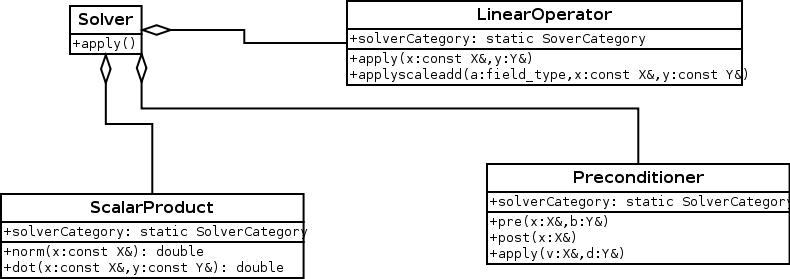
\includegraphics[width=\textwidth]{EPS/istlsolver}
\end{frame}

%-----------------------------------------------------------------------------

\begin{frame}
\frametitle{Parallel Preconditioners}
\begin{itemize}
\item To run in parallel Conjugate Gradients (CG) and BiCGStab solvers have to be able to compute parallel matrix vector
products and scalar products.
\item As parallel preconditioners to the CG and BiCGStab solvers additive Schwarz methods can be used:
\begin{itemize}
\item In this schemes the local subproblem on each processor is solved
where the values of the last iteration are used as Dirichlet constraints at the process boundary. 
\item Different solvers can be choosen for the local problems (e.g. a direct solver like SuperLU or some steps of an 
iterative solver like SSOR).
\item In an overlapping decomposition corrections are computed for the overlap at more than one process. The sum of the corrections multiplied with a relaxation 
coefficient is applied. 
\item With an overlapping Schwarz method the convergence is better the larger the overlap.
\end{itemize}
\item For overlapping domain decomposition there exists also an algebraic multigrid preconditioner.
\end{itemize}
\end{frame}


\begin{frame}
  \frametitle{Parallel Solver Backends for Overlapping DD}
The linear solvers in this table are preconditioned with an overlapping domain decomposition
using the respective smoother or with a parallel algebraic multigrid scheme with an SSOR smoother (AMG).
\begin{center}
\begin{tabular}{|l|l|l|}\hline
solver backend & smoother & linear solver\\\hline
\lstinline!ISTLBackend_OVLP_CG_SSORk<GFS,C>! & SSOR & CG\\\hline
\lstinline!ISTLBackend_OVLP_CG_SuperLU<GFS,C>! & SuperLU & CG\\\hline
\lstinline!ISTLBackend_CG_AMG_SSOR<GFS>! & AMG & CG\\\hline
\lstinline!ISTLBackend_OVLP_BCGS_SSORk<GFS,C>! & SSOR & BiCGStab\\\hline
\lstinline!ISTLBackend_OVLP_BCGS_SuperLU<GFS,C>! & SuperLU & BiCGStab\\\hline
\lstinline!ISTLBackend_BCGS_AMG_SSOR<GFS>! & AMG & BiCGStab\\\hline
\end{tabular}
\end{center}
\lstinline!ISTLBackend_OVLP_ExplicitDiagonal<GFS>! is a solver for explicit 
time-steppers with (block-)diagonal mass matrix.

The template parameter \lstinline!GFS! is the grid function space, \lstinline!C! is the type of the 
constraints container (usually \lstinline!OverlappingConformingDirichletConstraints!).
\end{frame}

\begin{frame}[fragile]
  \frametitle{Overlapping Example}
  \begin{lstlisting}[basicstyle=\small]
// 1. Create an overlapping grid
Dune::FieldVector<double,2> L(1.0);
Dune::FieldVector<int,2> N(16);
Dune::FieldVector<bool,2> periodic(false);
int overlap=2; 
Dune::YaspGrid<2> grid(helper.getCommunicator(),L,N,periodic,overlap);
typedef Dune::YaspGrid<2>::LeafGridView GV;
const GV& gv=grid.leafView();

// 2. Create correctly constrained grid function space
typedef Dune::PDELab::Q1LocalFiniteElementMap<Coord,Real,dim> FEM;
FEM fem;
typedef Dune::PDELab::OverlappingConformingDirichletConstraints CON;
typedef Dune::PDELab::ISTLVectorBackend<> VBE;
typedef Dune::PDELab::GridFunctionSpace<GV,FEM,CON,VBE> GFS;
GFS gfs(gv,fem);

//  define problem parameters
typedef ConvectionDiffusionProblem<GV,Real> Param;
Param param;
typedef Dune::PDELab::BoundaryConditionType_CD<Param> B;
B b(gv,param);
typedef Dune::PDELab::DirichletBoundaryCondition_CD<Param> G;
G g(gv,param);
\end{lstlisting}  
\end{frame}
\begin{frame}[fragile]
\frametitle<presentation>{Overlapping Example Continued}
  \begin{lstlisting}[basicstyle=\small]

//  Compute constrained space
typedef typename GFS::template ConstraintsContainer<Real>::Type C;
C cg;
Dune::PDELab::constraints(b,gfs,cg);
// Make grid operator space
typedef Dune::PDELab::ConvectionDiffusion<Param> LOP;
LOP lop(param,2);
typedef Dune::PDELab::ISTLMatrixBackend MBE;
typedef Dune::PDELab::GridOperator<GFS,GFS,LOP,MBE,double,double,double,C,C> GO;
GO go(gfs,cg,gfs,cg,lop);

//  Compute affine shift
typedef typename GO::Traits::Domain V;
V x(gfs,0.0);
Dune::PDELab::interpolate(g,gfs,x);
Dune::PDELab::set_nonconstrained_dofs(cg,0.0,x);

// 3. Choose a linear solver 
typedef Dune::PDELab::ISTLBackend_OVLP_BCGS_SuperLU<GFS,C> LS;
LS ls(gfs,cg,5000,2);
...
\end{lstlisting}
\end{frame}

\begin{frame}
  \frametitle{Parallel Solver Backends for Nonoverlapping DD}
The linear solvers in this table are preconditioned with a nonoverlapping domain decomposition
using the respective smoother.
\begin{center}
\begin{tabular}{|l|l|l|}\hline
solver backend & smoother & linear solver\\\hline
\lstinline!ISTLBackend_NOVLP_CG_NOPREC<GFS>! & -- & CG\\\hline
\lstinline!ISTLBackend_NOVLP_CG_Jacobi<GFS>! & Jacobi & CG\\\hline
\lstinline!ISTLBackend_NOVLP_CG_SSORk<GOS,Scalar>! & SSOR & CG\\\hline
\lstinline!ISTLBackend_NOVLP_BCGS_NOPREC<GFS>! & -- & BiCGStab\\\hline
\lstinline!ISTLBackend_NOVLP_BCGS_SSORk<GOS,Scalar>! & SSOR & BiCGStab\\\hline
\end{tabular}
\end{center}
\lstinline!ISTLBackend_NOVLP_ExplicitDiagonal! is a solver for explicit 
time-steppers with (block-)diagonal mass matrix.

The template parameter \lstinline!GFS! is the grid function space, \lstinline!GOS! is the grid operator space
and \lstinline!Scalar! the type of a scalar value in the matrix.
\end{frame}

\begin{frame}[fragile]
  \frametitle{Nonoverlapping example}
  \begin{lstlisting}[basicstyle=\small]
// 1. Create an non-overlapping grid
Dune::FieldVector<double,2> L(1.0);
Dune::FieldVector<int,2> N(16);
Dune::FieldVector<bool,2> periodic(false);
int overlap=0; // needs overlap 0 because overlap elements are not assembled
Dune::YaspGrid<2> grid(helper.getCommunicator(),L,N,periodic,overlap);
typedef Dune::YaspGrid<2>::LeafGridView GV;
const GV& gv=grid.leafView();

// 2. Create correctly constrained grid function space
typedef Dune::PDELab::Q1LocalFiniteElementMap<Coord,Real,dim> FEM;
FEM fem;
typedef Dune::PDELab::NonoverlappingConformingDirichletConstraints CON;
CON con;
typedef Dune::PDELab::ISTLVectorBackend<> VBE;
typedef Dune::PDELab::GridFunctionSpace<GV,FEM,CON,VBE> GFS;
GFS gfs(gv,fem,con);
con.compute_ghosts(gfs); // con stores indices of ghost dofs
typedef ConvectionDiffusionProblem<GV,Real> Param;
Param param;
typedef Dune::PDELab::BoundaryConditionType_CD<Param> B;
B b(gv,param);
typedef Dune::PDELab::DirichletBoundaryCondition_CD<Param> G;
G g(gv,param);
\end{lstlisting}
\end{frame}
\begin{frame}[fragile]
\frametitle<presentation>{Nonoverlapping Example Continued}
  \begin{lstlisting}[basicstyle=\small]
// Compute constrained space
typedef typename GFS::template ConstraintsContainer<Real>::Type C;
C cg;
Dune::PDELab::constraints(b,gfs,cg);

// Make grid operator space
typedef Dune::PDELab::ConvectionDiffusion<Param> LOP;
LOP lop(param,2);
typedef Dune::PDELab::ISTLMatrixBackend MBE;
typedef Dune::PDELab::GridOperator<GFS,GFS,LOP,MBE,double,double,double,C,C,true> GO;
GO gos(gfs,cg,gfs,cg,lop);

// Compute affine shift
typedef typename GO::Traits::Domain V;
V x(gfs,0.0);
Dune::PDELab::interpolate(g,gfs,x);
Dune::PDELab::set_nonconstrained_dofs(cg,0.0,x);

// 3. Choose a linear solver 
typedef Dune::PDELab::ISTLBackend_NOVLP_BCGS_NOPREC<GFS> LS;
LS ls(gfs,5000,1);
...
\end{lstlisting}
  
\end{frame}

}
\mode<all>{\section{Using Adaptivity and Local Refinement}

\subsection{Adaptivity in general}

\subsubsection*{What is adaptivity all about?}

\begin{frame}
  \frametitle<presentation>{What is adaptivity all about?}
  \begin{center}
    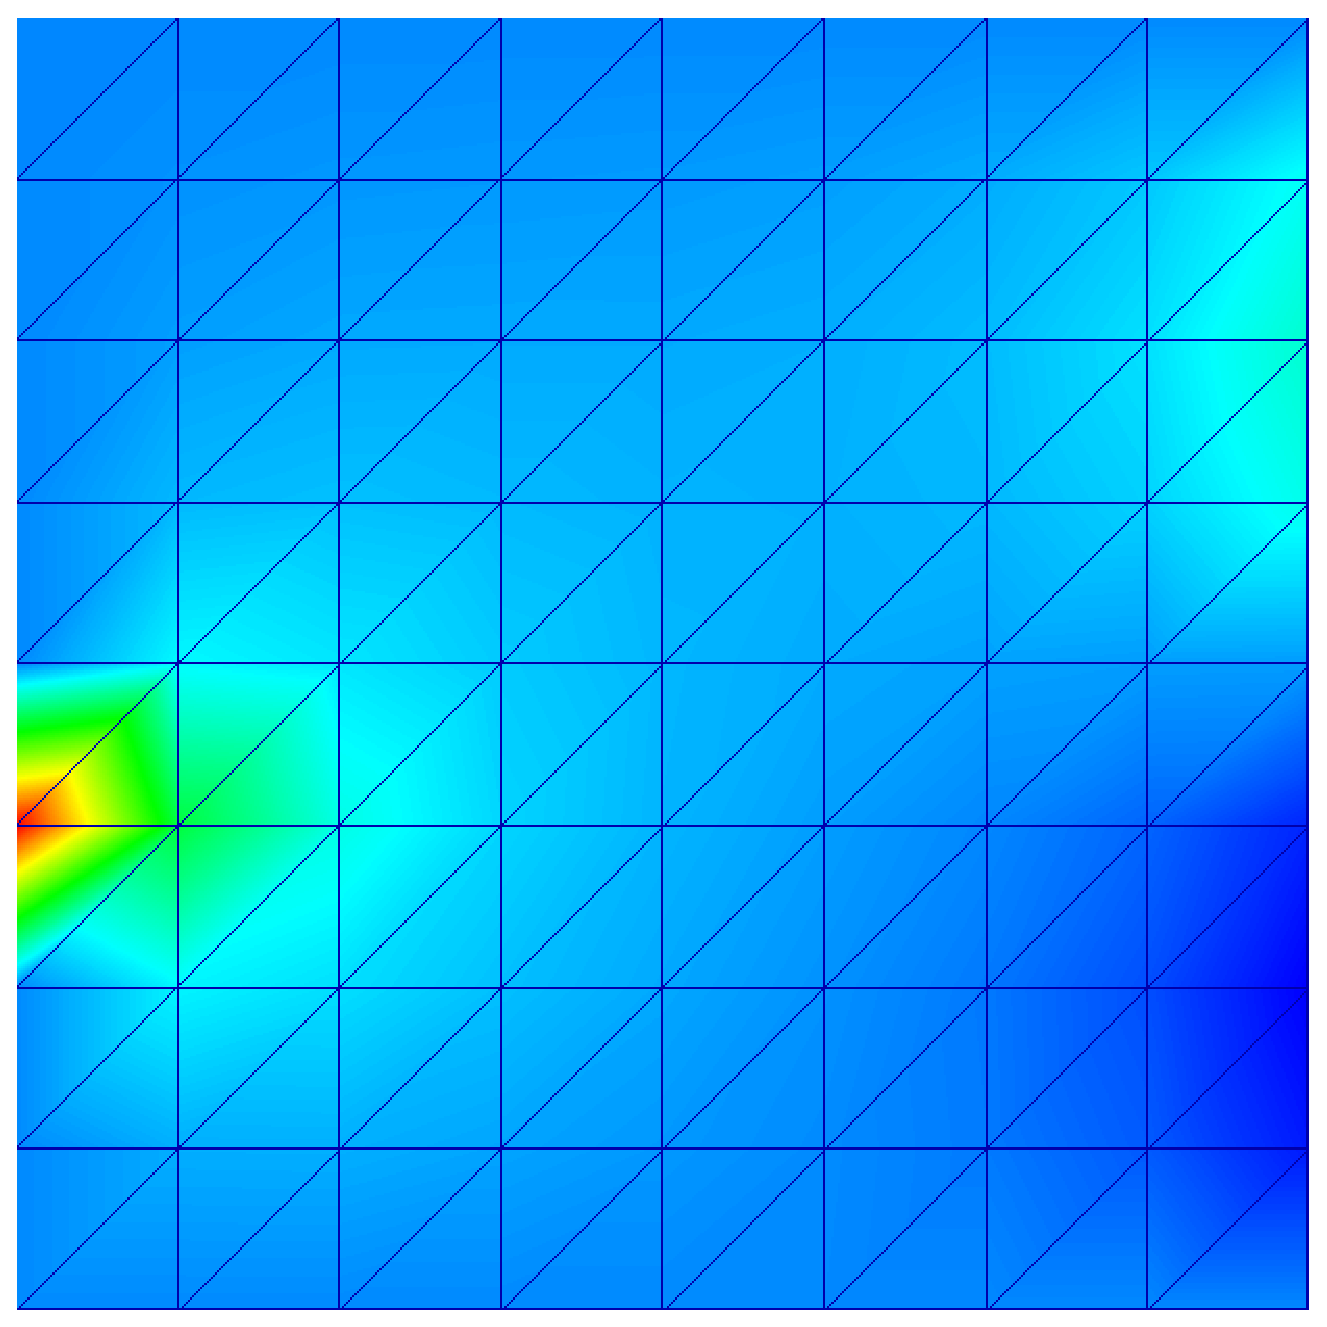
\includegraphics[width=0.4\textwidth]{EPS/adaptivity/low_resolution}

    A coarse discretisation may not be able to capture \\ all the features of the solution \ldots

    \begin{tabular}{rl}
      $h$:          & $2^{-3}$ \\
      DOF:          & 81       \\
      Time (total): & 0.026 s
    \end{tabular}
  \end{center}
\end{frame}

\begin{frame}
  \frametitle<presentation>{What is adaptivity all about?}
  \begin{center}
    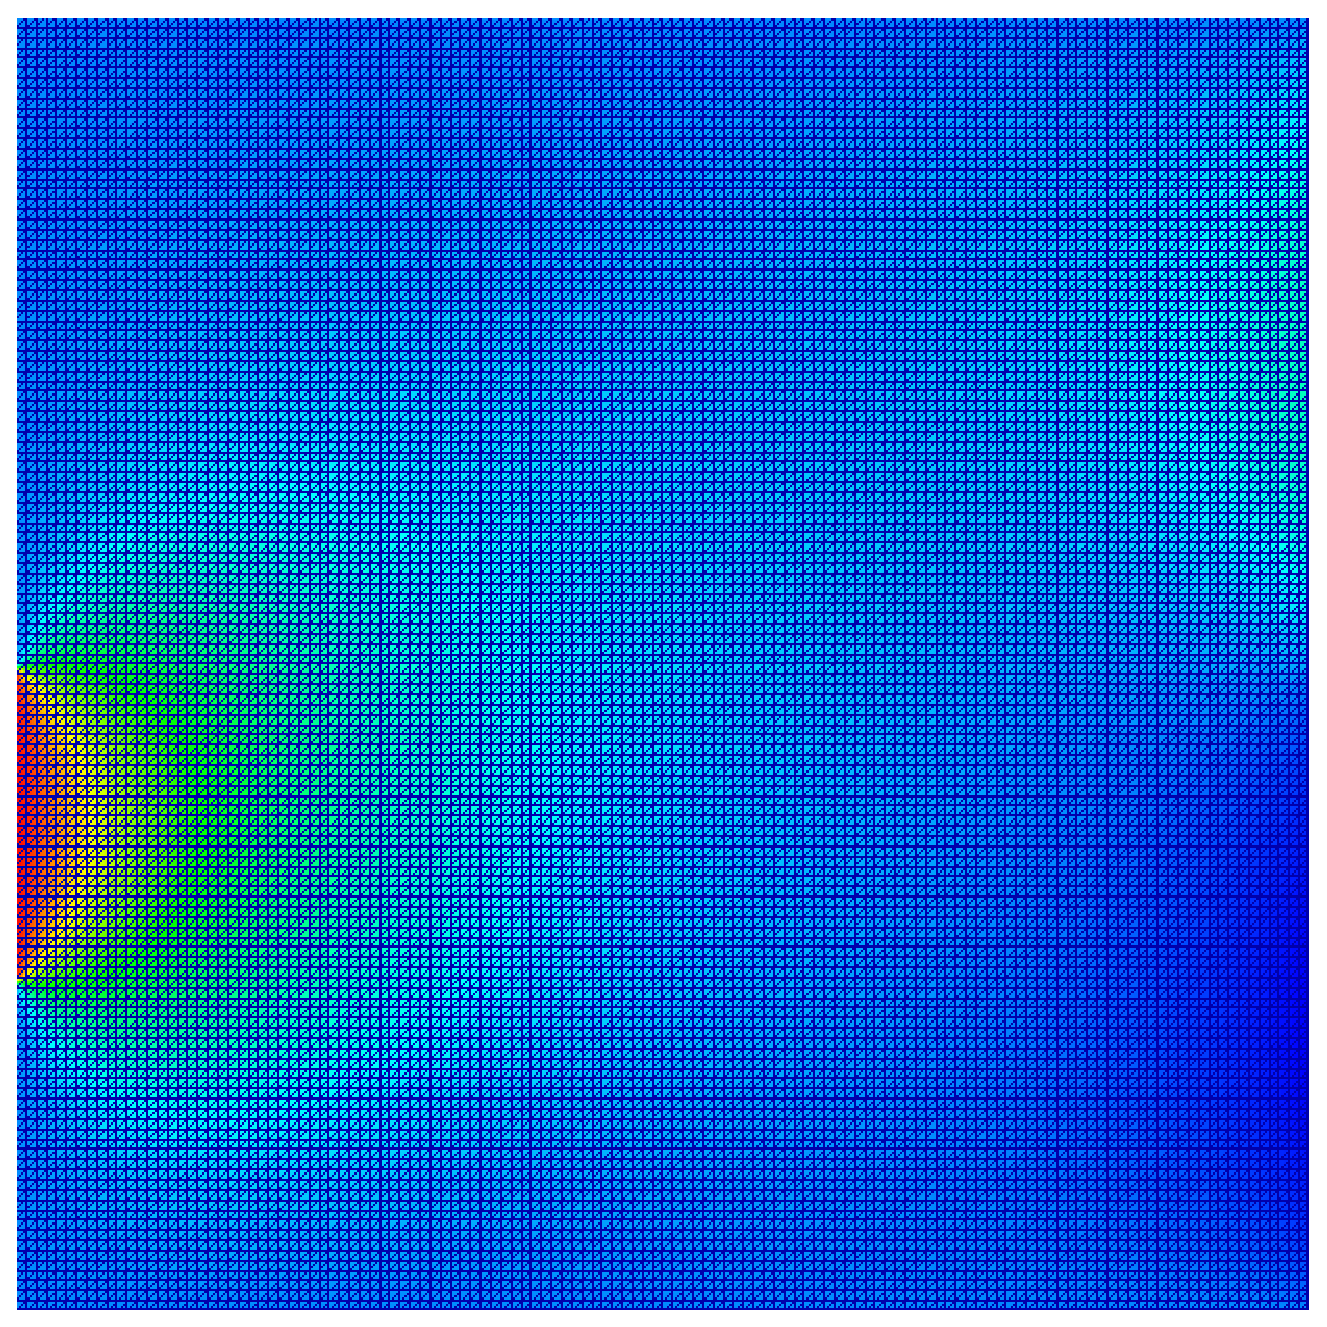
\includegraphics[width=0.4\textwidth]{EPS/adaptivity/high_resolution}

    \ldots while a fine discretisation may have \\ too many degrees of freedom to be feasable.

    \begin{tabular}{rl}
      $h$:          & $2^{-7}$ \\
      DOF:          & 16641    \\
      Time (total): & 38.3 s
    \end{tabular}
  \end{center}
\end{frame}

\begin{frame}<presentation>
  \frametitle<presentation>{What is adaptivity all about?}
  \begin{center}

    \only<1>{
    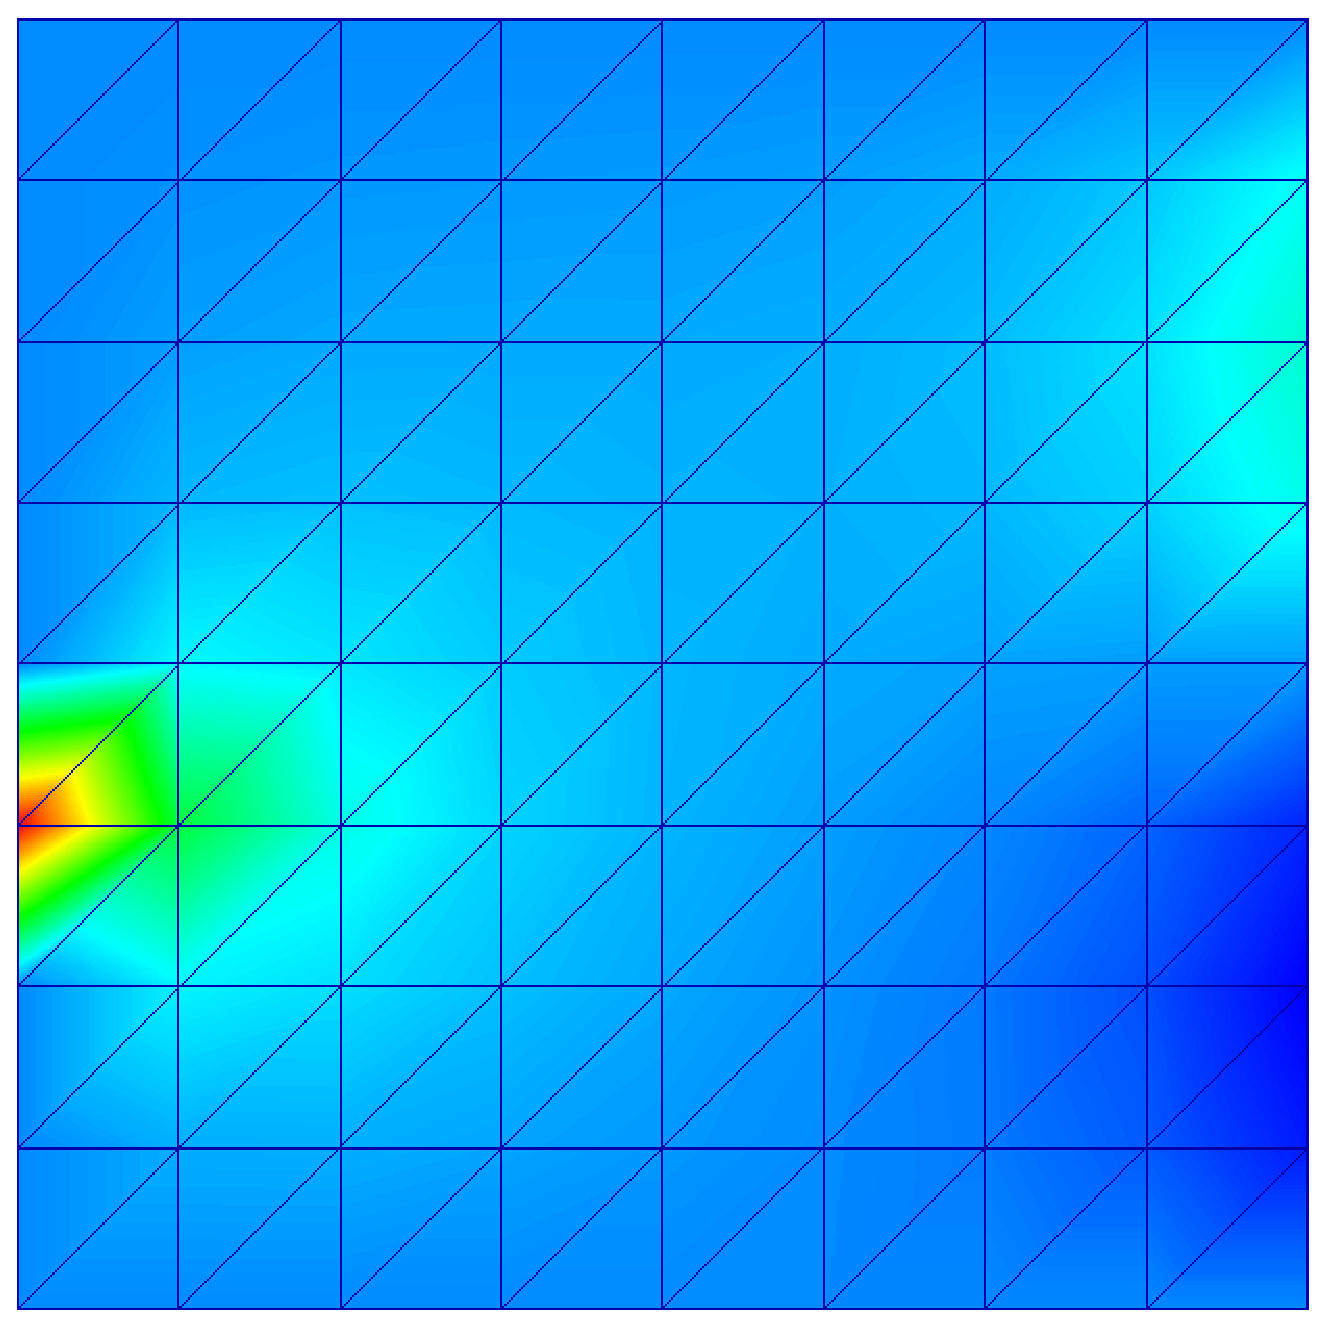
\includegraphics[width=0.4\textwidth]{EPS/adaptivity/adaptivity1}
    }

    \only<2>{
    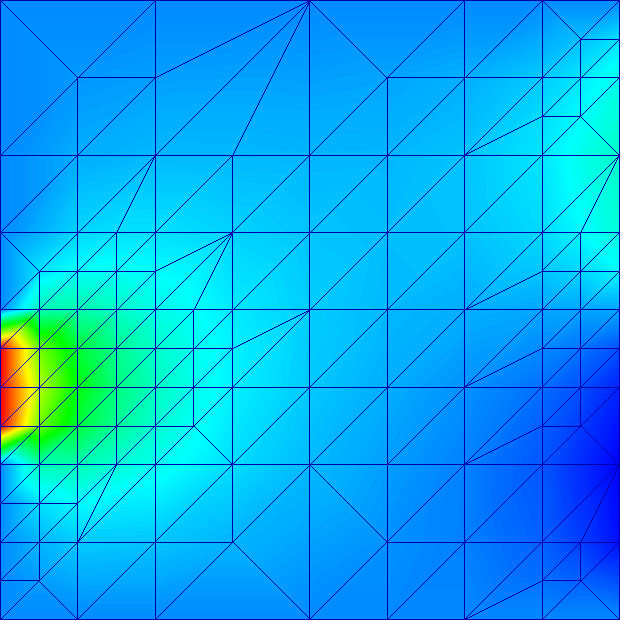
\includegraphics[width=0.4\textwidth]{EPS/adaptivity/adaptivity2}
    }

    \only<3>{
    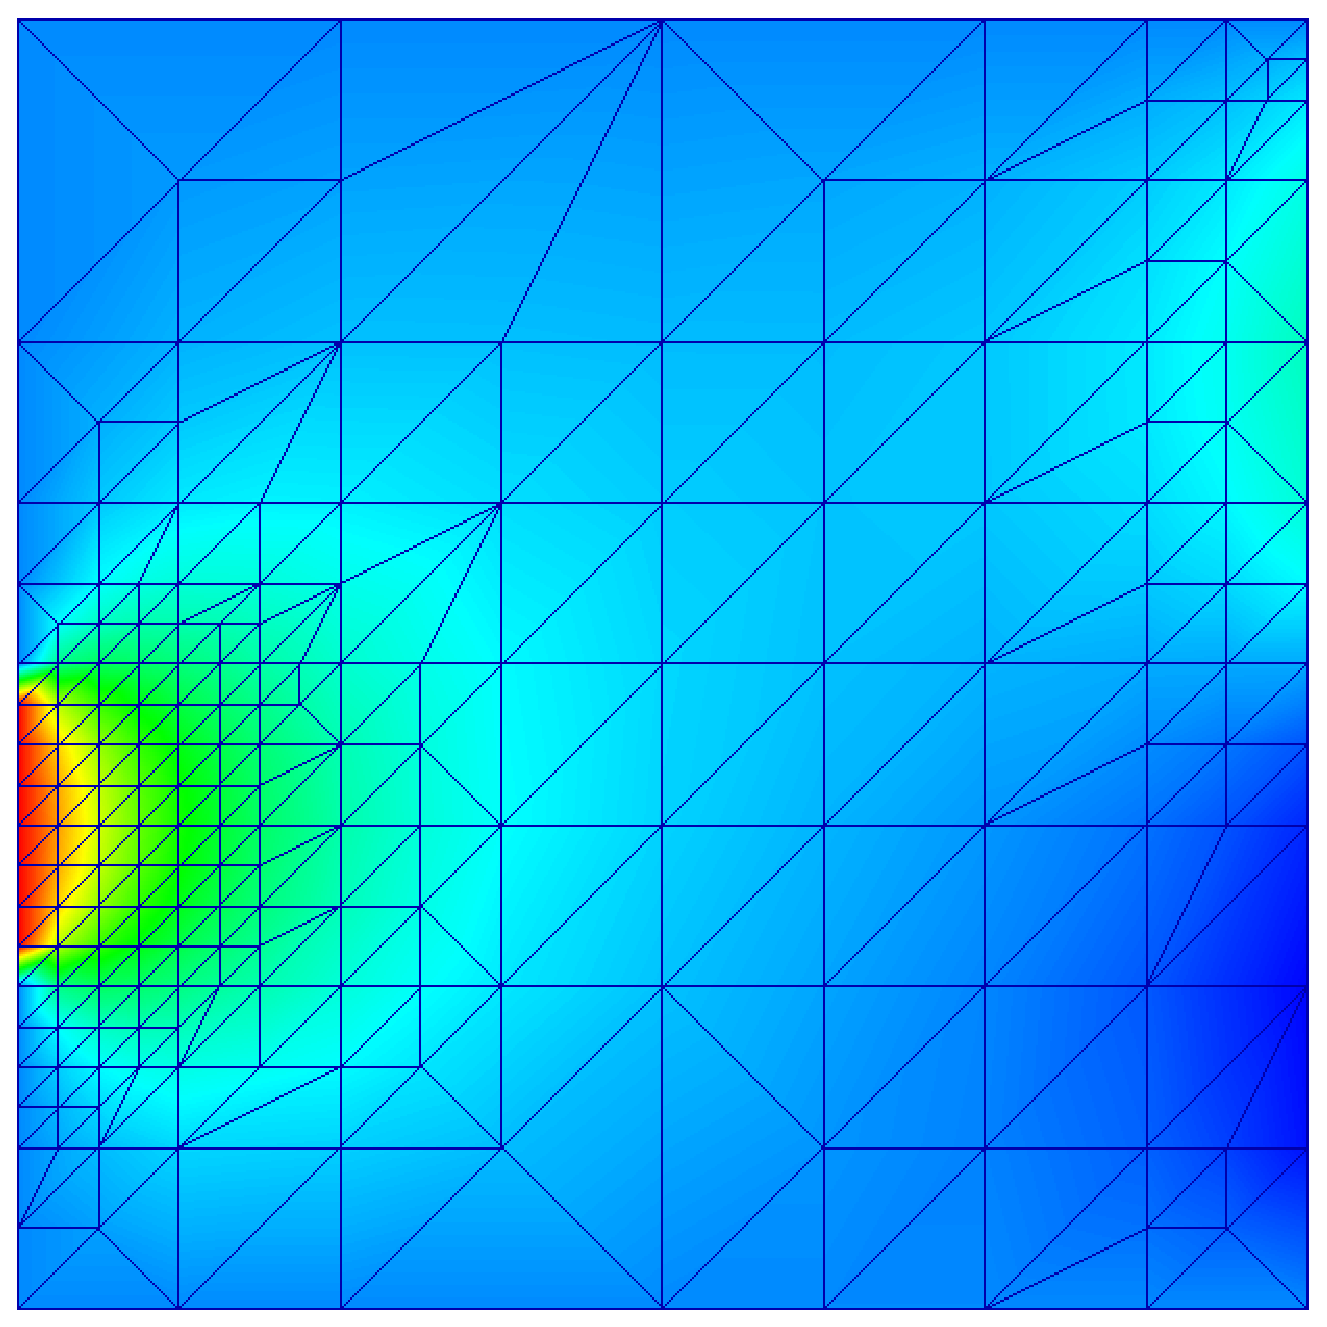
\includegraphics[width=0.4\textwidth]{EPS/adaptivity/adaptivity3}
    }

    \only<4>{
    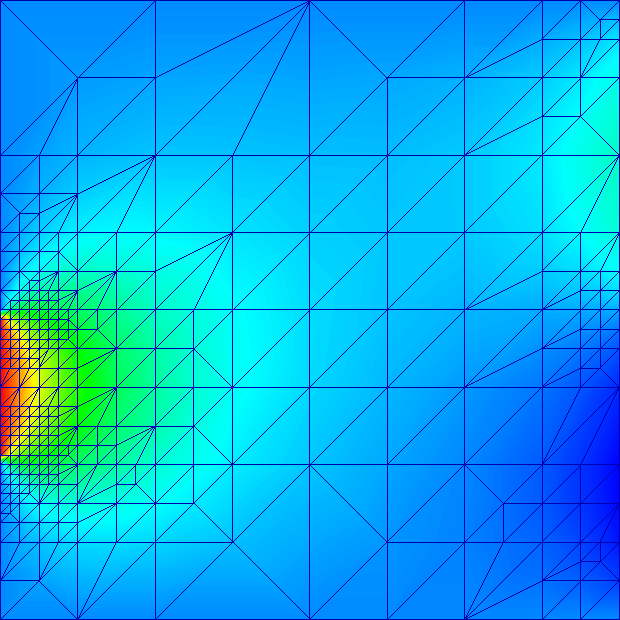
\includegraphics[width=0.4\textwidth]{EPS/adaptivity/adaptivity4}
    }

    \only<5>{
    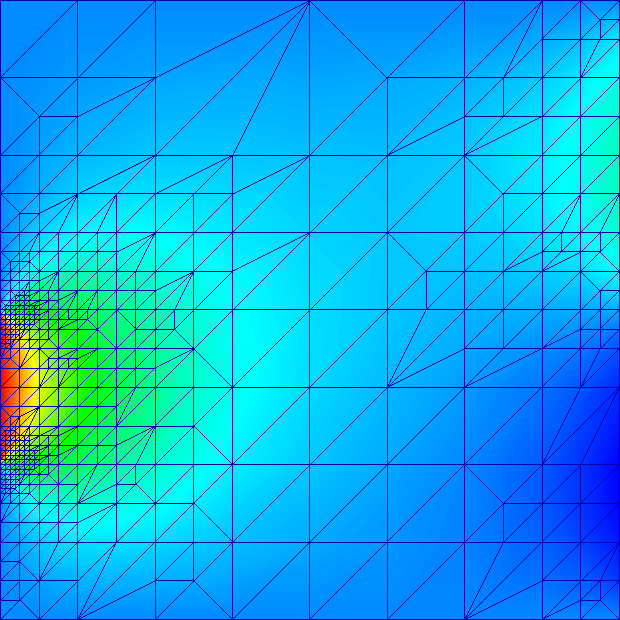
\includegraphics[width=0.4\textwidth]{EPS/adaptivity/adaptivity5}
    }

    \emph{Idea:} Use a higher resolution only in areas where it is beneficial.

    \only<1>{
    \begin{tabular*}{0.95\textwidth}{rl}
      $h_{\min}$:   & $2^{-3}$ \\ 
      DOF:          & 81       \\
      Time (total): & 0.026s
    \end{tabular*}
    }

    \only<2>{
    \begin{tabular*}{0.95\textwidth}{rl}
      $h_{\min}$:   & $2^{-4}$                         \\
      DOF:          & 81 + 124        = \alert{205}    \\
      Time (total): & 0.026s + 0.059s = \alert{0.085s}
    \end{tabular*}
    }

    \only<3>{
    \begin{tabular*}{0.95\textwidth}{rl}
      $h_{\min}$:   & $2^{-5}$                                  \\
      DOF:          & 81 + 124 + 200           = \alert{405}    \\
      Time (total): & 0.026s + 0.059s + 0.090s = \alert{0.175s}
    \end{tabular*}
    }

    \only<4>{
    \begin{tabular*}{0.95\textwidth}{rl}
      $h_{\min}$:   & $2^{-6}$                                          \\
      DOF:          & 81 + 124 + 200 + 323             = \alert{728}    \\
      Time (total): & 0.026s + 0.059s + 0.090s + 0.15s = \alert{0.325s}
    \end{tabular*}
    }

    \only<5>{
    \begin{tabular*}{0.95\textwidth}{rl}
      $h_{\min}$:   & $2^{-7}$                                                  \\
      DOF:          & 81 + 124 + 200 + 323 + 506               = \alert{1234}   \\
      Time (total): & 0.026s + 0.059s + 0.090s + 0.15s + 0.27s = \alert{0.595s}
    \end{tabular*}
    }

  \end{center}
\end{frame}

\begin{frame}<article>
  \begin{center}

    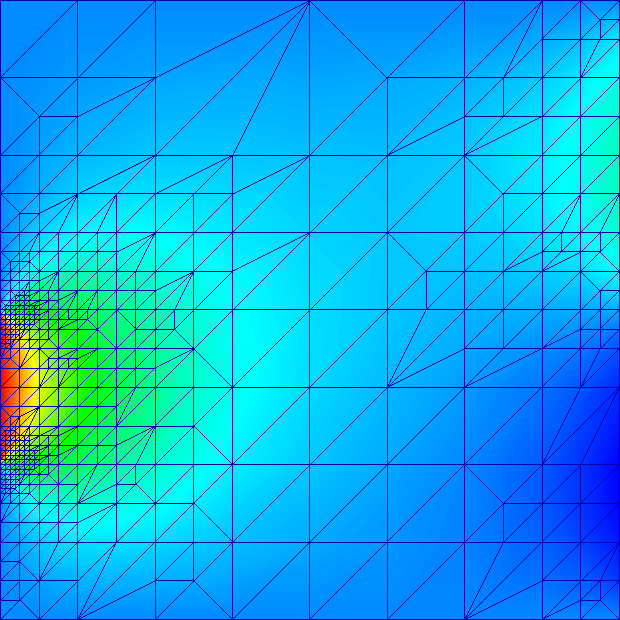
\includegraphics[width=0.4\textwidth]{EPS/adaptivity/adaptivity5}

    \emph{Idea:} Use a higher resolution only in areas where it is beneficial.

    \begin{tabular*}{0.95\textwidth}{rl}
      $h_{\min}$:   & $2^{-7}$                                                  \\
      DOF:          & 81 + 124 + 200 + 323 + 506               = \alert{1234}   \\
      Time (total): & 0.026s + 0.059s + 0.090s + 0.15s + 0.27s = \alert{0.595s}
    \end{tabular*}

  \end{center}
\end{frame}

\begin{frame}
  \frametitle<presentation>{What is adaptivity all about?}
  \begin{center}
    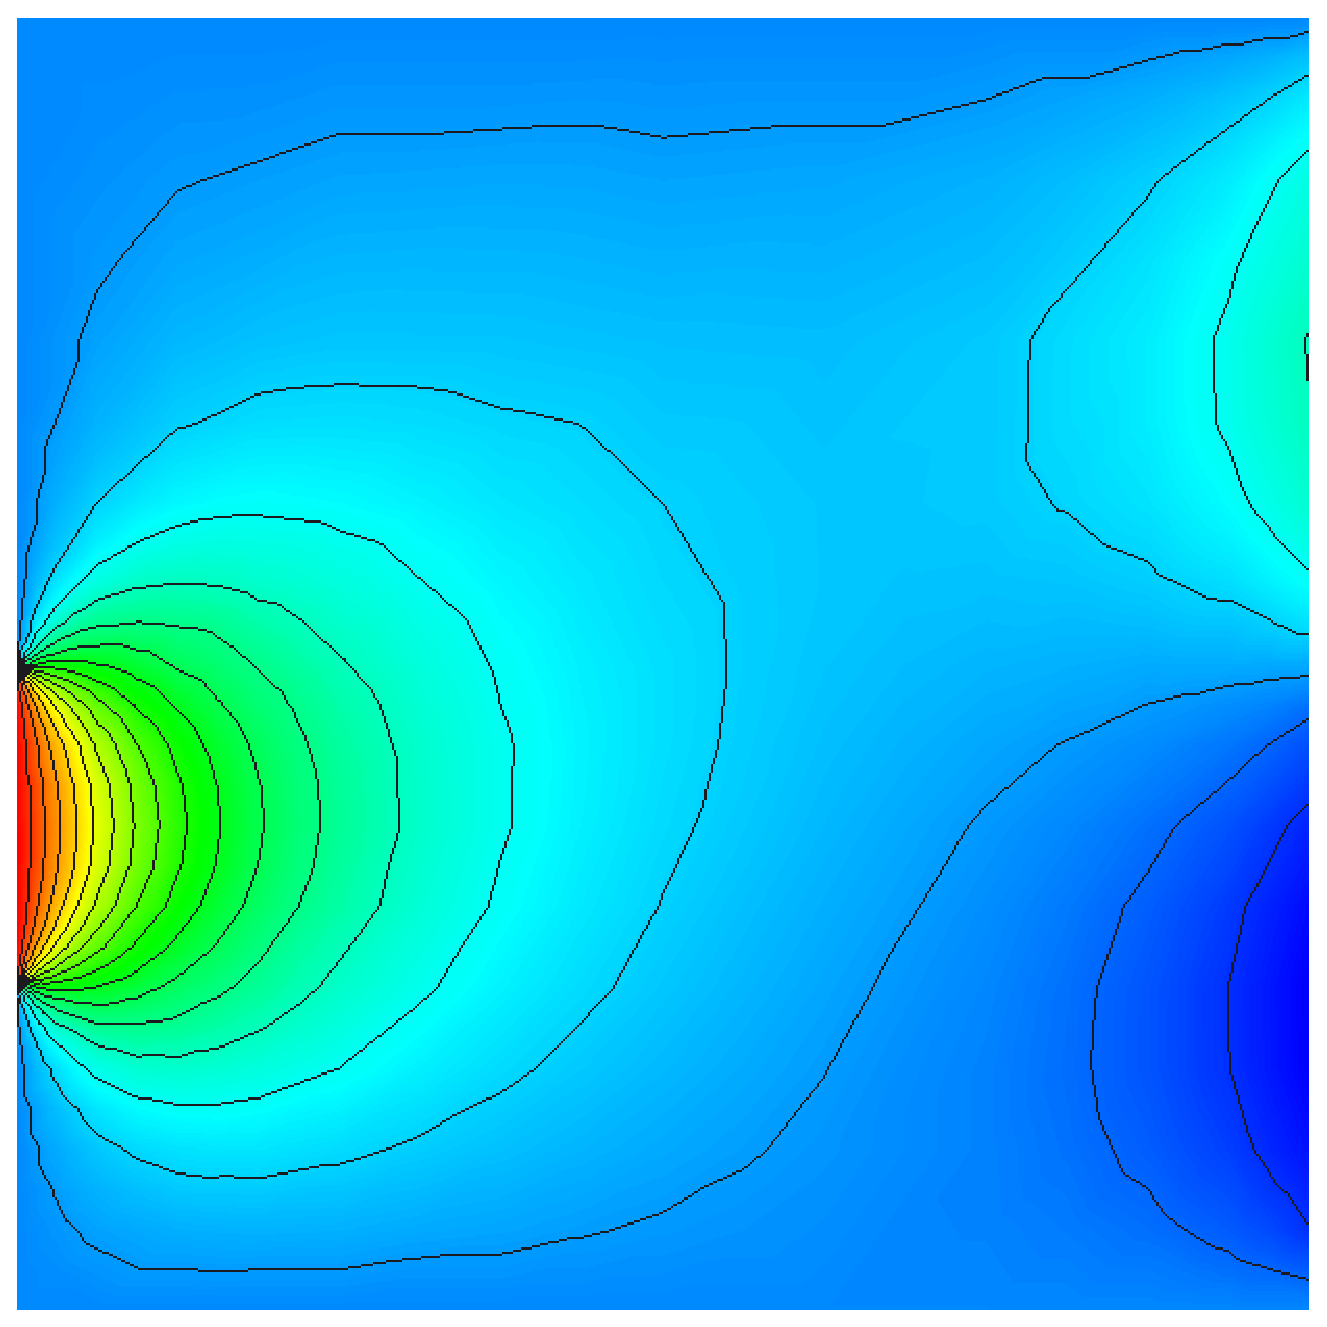
\includegraphics[width=.45\textwidth]{EPS/adaptivity/adaptive_iso} \hfill
    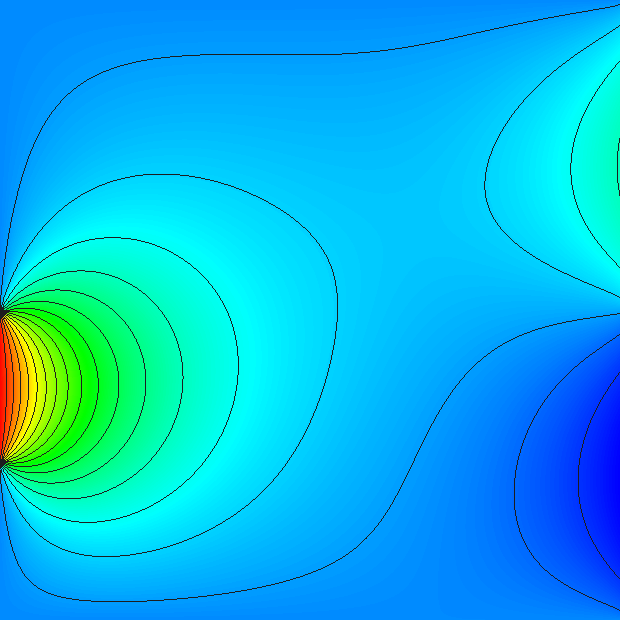
\includegraphics[width=.45\textwidth]{EPS/adaptivity/fine_iso}

    Adaptive     \hfill \hspace{7ex}Local refinement may lead to   \hfill Globally refined

    506 DOFs     \hfill \hspace{3ex}similar results using far less \hfill 16641 DOFs

    \alert{0.6s} \hfill computational effort.                      \hfill \alert{38s}

  \end{center}
\end{frame}

\begin{frame}
  \frametitle<presentation>{What is adaptivity all about?} 

  Adaptive Scheme
  \[
  (\mathbb{T}_n,C_{n}) \stackrel{\nu_n}{\rightarrow} (\mathbb{T}_{n+1},C_{n+1})
  \]

  Combined with \emph{error control}, adaptivity aims for optimization of the computational effort with a constraint on the maximum tolerated discretization error.

  \begin{block}{Adaptation goals}
    \begin{itemize}
      \item enhance accuracy in a localized manner
      \item reduce cost of the simulation.
    \end{itemize}
  \end{block}
\end{frame}

\begin{frame}
  \frametitle<presentation>{What is adaptivity all about?}
  \begin{block}{\emph{Main Problem}}
    How do we decide which regions are to be refined?

    It would be best to e.g.~spread the discretisation error evenly over the domain.
  \end{block}

  \pause
  \begin{block}{\emph{Solution}}
    Implement an \emph{\emph{error estimator}} with local \emph{\emph{error indicators}} computing a rough estimate of the discretisation error and refine regions with high local error.
  \end{block}

  Error estimators are taylored to the problem at hand, and the creation of \emph{efficient} error estimators is an active area of research.
\end{frame}

\begin{frame}[fragile]
  \frametitle<presentation>{Error Indication}

  \begin{center}
    \begin{minipage}{0.75\textwidth}
      \begin{center}
        Error indication by maximal concentration difference

        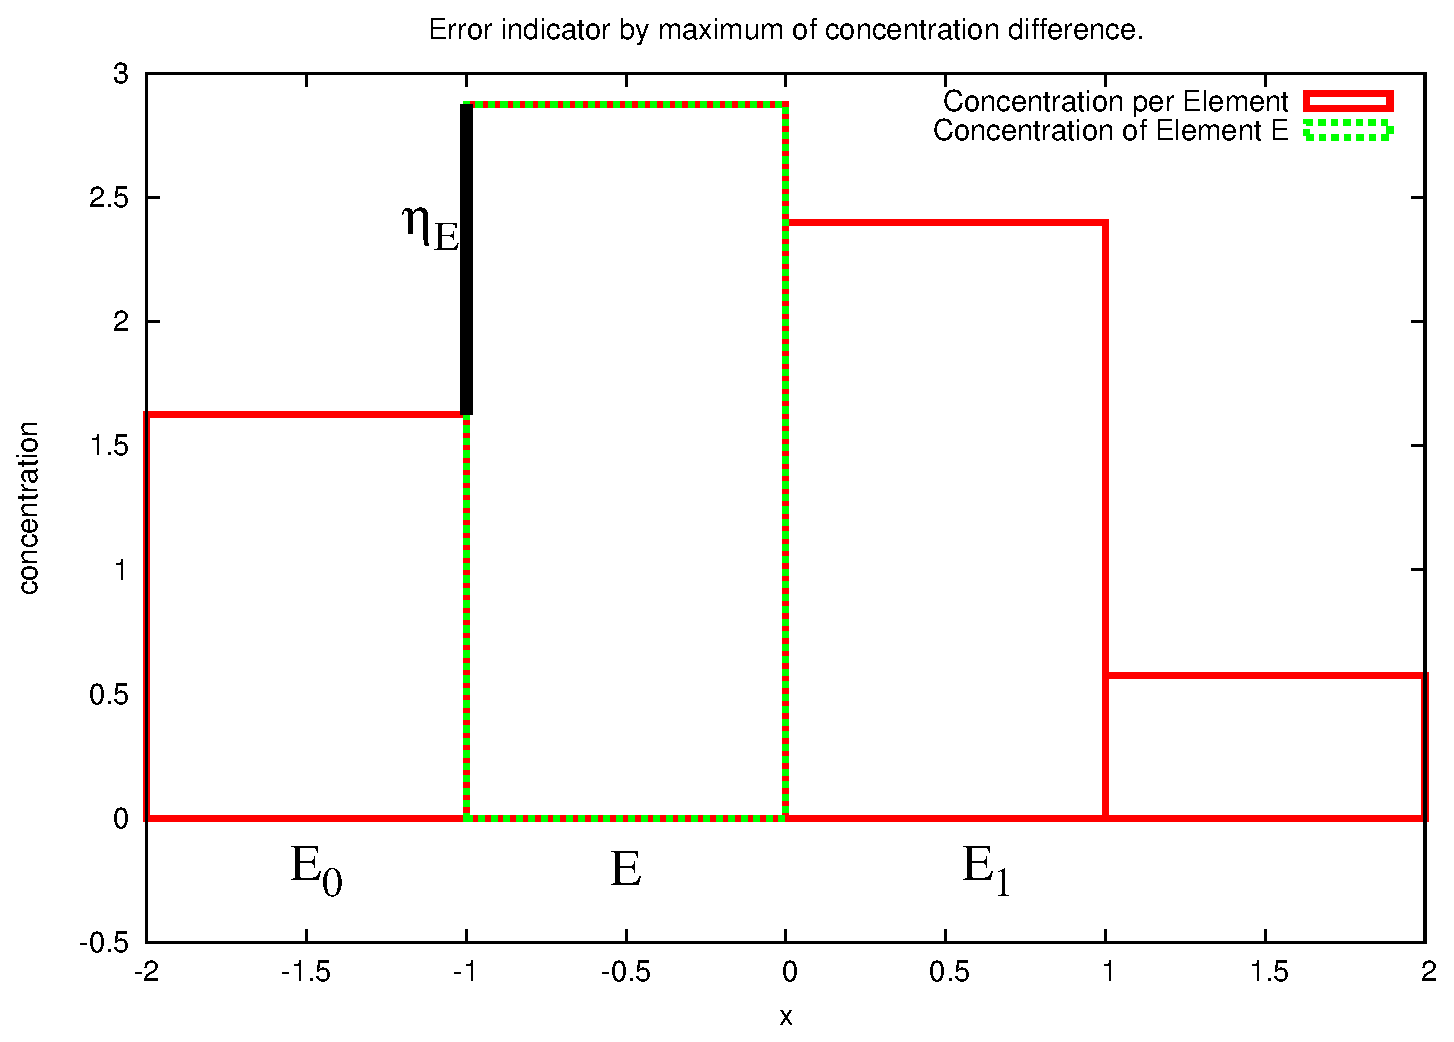
\includegraphics[width=0.95\textwidth]{EPS/adaptivity/errind_maxconc}
      \end{center}
    \end{minipage}
  \end{center}
\end{frame}

\begin{frame}
  \frametitle<presentation>{What is adaptivity all about?}
  There are two main ways to increase the local resolution:
  \begin{itemize}
    \item Use smaller elements at the points of interest (\emph{$h$-Refinement})
    \item Increase the polynomial degree of the elements (\emph{$p$-Refinement})
  \end{itemize}

  The two approaches can be combined, of course. This is called $hp$-Refinement.

  We will focus on $h$-Refinement.

\end{frame}

\subsection{$h$-Refinement}

\begin{frame}
  \frametitle<presentation>{$h$-Refinement}
  In \emph{$h$-Refinement}, the mesh size $h$ is decreased in areas that need a high resolution. To achieve this, the cells in the affected areas are replaced by cells with a \emph{smaller diameter}.

  There are several different strategies for finding a suitable refinement. Things to consider are e.g.~the \emph{construction effort} and the \emph{quality} of the resulting cells (anisotropy, inner angles, distance between nodes\ldots).

  We will have a look at
  \begin{itemize}
    \item Edge Bisection
    \item Red-Green Refinement
  \end{itemize}
\end{frame}

\subsubsection*{Bisection}

\begin{frame}
  \frametitle<presentation>{Edge Bisection}
  \begin{center}
    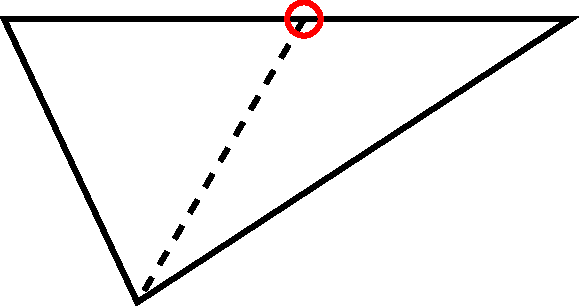
\includegraphics[width=0.45\textwidth]{EPS/adaptivity/bisection}
  \end{center}
  \begin{itemize}
    \item each element is split into two
    \item choice of edge is important: \newline
      bisection of the shortest edge will lead to poor mesh quality
    \item used in \emph{AlbertaGrid}
  \end{itemize}
\end{frame}

\subsubsection*{Red-Green Refinement}

\begin{frame}
  \frametitle<presentation>{Red-Green Refinement}
  \begin{center}
    \includegraphics[width=0.45\textwidth]{EPS/adaptivity/redgreen}
  \end{center}
  \begin{itemize}
    \item is also called \emph{regular refinement}
    \item used in \emph{ALUGrid} and \emph{UGGrid}
    \item simplicial case (triangle, tetrahedron): \newline
      new vertices are placed in the center of edges,
    \item quadrilateral, hexadron: new vertices are placed in the center of edges, sides and volumes
    \item results are \emph{similar} (i.e.~congruent up to scaling)
  \end{itemize}
\end{frame}

\begin{frame}
  \frametitle{Regular Refinement of Elements}

  \begin{center}
    \begin{minipage}{0.8\textwidth}
      \begin{center}
        \includegraphics[width=0.45\linewidth]{EPS/adaptivity/refinetet}
        \hfill
        \includegraphics[width=0.45\linewidth]{EPS/adaptivity/refinepyr}\\

        Tetrahedron \hspace*{3cm} Pyramid
      \end{center}
      \vspace{0.5cm}
      \begin{center}
        \includegraphics[width=0.45\linewidth]{EPS/adaptivity/refinepri}
        \hfill
        \includegraphics[width=0.45\linewidth]{EPS/adaptivity/refinehex}

        Prism \hspace*{3cm} Hexahedron
      \end{center}
    \end{minipage}
  \end{center}
\end{frame}


\subsubsection*{Hanging nodes}

\begin{frame}
  \frametitle<presentation>{Hanging Nodes}

  \begin{center}
    \includegraphics[width=0.95\textwidth]{EPS/adaptivity/hanging}
  \end{center}

  Local refinement may lead to so called hanging nodes, sitting on the edge of a coarser element.

  In contrast to regular nodes, hanging nodes may not be true degrees of freedom, e.g.~in the case of a conforming ansatz space.
\end{frame}

\begin{frame}
  \frametitle<presentation>{Hanging Nodes}
  \includegraphics[width=\linewidth]{EPS/adaptivity/hexclosurenew}

  \begin{block}{Conforming Closure}
    \begin{itemize}
      \item Regular (red), irregular (green) and copy (yellow) refinements
      \item Conforming closure for each possible situation ($2^{19}$ cases for hexahedra)
      \item no iteration process necessary $\rightarrow$ well suited for parallelization
    \end{itemize}
  \end{block}
\end{frame}

\subsection{Adaptivity in DUNE}

\subsubsection*{Workflow}

\begin{frame}<presentation>
  \frametitle{Grid Access: Viewing vs. Modification}
  The DUNE Grid interface follows the \emph{View-only} Concept.
  \pause
  \only<presentation>{\vfill}
  \structure{View-Only Concept}
  \begin{itemize}
    \item Views offer (read-only) access to the data
      \begin{itemize}
        \item Read-only access to grid entities allow the consequent use of const.
        \item Access to entities is only through iterators for a
          certain view. 
          \begin{itemize}
            \item[$\Rightarrow$] \emph{This allows on-the-fly implementations.}
          \end{itemize}
      \end{itemize}
    \item  Data can only be modified in the primal container \emph{(the Grid)}
  \end{itemize}
  \pause
  \only<presentation>{\vfill}
  \structure{Modification Methods:}
  \begin{itemize}
    \item  Global Refinement

    \item  \textcolor{red}{Local Refinement \& Adaptation}

    \item  Load Balancing
  \end{itemize}
\end{frame}

\begin{frame}
  \frametitle<presentation>{Marking Elements} 

  {\bf First phase:} {Marking of elements}
  \begin{itemize}
    \item The method\newline
      \lstinline{bool mark (int refCount, const Codim<0>::Entity& e)}\newline
      is used to mark an entity \lstinline{e} for 
      \begin{itemize}
        \item refinement (refCount $> 0$) or 
        \item coarsening (refCount $< 0$)
        \item neither (refCount = 0).
      \end{itemize}
      It returns \lstinline{true} if the counter has been updated
      successfully.
    \item  Calling the method\newline
      \lstinline{int getMark (const Codim<0>::Entity& e) const}\newline
      returns the current refinement counter of an entity.
  \end{itemize}
\end{frame}

\begin{frame}
  \frametitle<presentation>{Grid Adaptation} 

  {\bf Second phase:} {Grid modification}
  \begin{enumerate}
    \item Call the grid's method \lstinline{grid.preAdapt()}. This method \emph{prepares}
      the grid for adaptation. It returns \lstinline{true} if at least one entity was
      marked for coarsening.

      \pause

    \item If \lstinline{grid.preAdapt()} returned \lstinline{true}, any data associated with
      entities that might be coarsened during the following adaptation
      cycle has to be \emph{projected} to the father entities.

      \pause

    \item Call \lstinline{grid.adapt()}. The grid is \emph{modified} according to the
      adaptation marks.

      \pause

    \item If \lstinline{grid.adapt()} returned \lstinline{true}, new entities were created.
      Existing data must be \emph{prolongated} to newly created entities.

      \pause

    \item Call \lstinline{grid.postAdapt()} to \emph{clean up} refinement markers.
  \end{enumerate}

  \pause

  As the data management is the user's responsibility, he or she has to
  take care of restriction and prolongation of data attached to the grid. 
  This is possible using the persistent index maps 
  i.\,e., \lstinline{LocalIdSet} and \lstinline{GlobalIdSet}.
\end{frame}

\begin{frame}
  \frametitle{Data Transfer between Grids}

  The {\sc Dune} \lstinline{Entity<0>} class provides two methods, which are
  needed during the grid modification phase for solution transfer:
  \begin{itemize}
    \item The method\newline
      \lstinline{bool mightVanish () const}\newline
      returns \lstinline{true} if the entity {\bf \emph{might}} be removed when
      \lstinline{grid.adapt()} is called. 

      \pause

    \item The method\newline
      \lstinline{bool isNew () const}\newline
      returns \lstinline{true} if the entity was newly generated in the
      grid modification process, otherwise \lstinline{false}.
  \end{itemize}

  \pause

  \begin{block}{\emph{Note:}}
    Both methods may only be called between \lstinline{grid.preAdapt()}
    and \lstinline{grid.postAdapt()}.
  \end{block}

\end{frame}

\begin{frame}
  \frametitle{Solution Transfer during Adaptation I}  

  \begin{center}
    \includegraphics[width=0.9\textwidth]{EPS/adaptivity/hadapt}
  \end{center}

\end{frame}

\begin{frame}
  \frametitle{Solution Transfer during Adaptation II}  

  \begin{center}
    \includegraphics[width=0.8\textwidth]{EPS/adaptivity/hadapt1}
  \end{center}

\end{frame}

\begin{frame}
  \frametitle<presentation>{Summary}
  \begin{block}{\emph{Summary}}
    \begin{enumerate}
      \item mark the appropriate cells
      \item backup/project your data (preAdapt, mightVanish-Flags)
      \item adapt the grid proper
      \item restore/interpolate your data (postAdapt, isNew-Flags)
    \end{enumerate}
  \end{block}
  \pause
  \begin{block}{\emph{But:}}
    PDELab does all of this for you!
  \end{block}
\end{frame}

\subsubsection*{The Grids and their abilities}

\paragraph{YaspGrid}

\begin{frame}
  \frametitle<presentation>{YaspGrid}
  \begin{center}
    \includegraphics{EPS/adaptivity/cartesian}
  \end{center}
  \begin{block}{\emph{YaspGrid}}
    is used in most of the examples.

    It is a \emph{Cartesian} grid, i.e.~a tensor grid with equidistant spacing in each dimension, and therefore \emph{cannot} be locally refined.
  \end{block}
\end{frame}

\paragraph{Other Grids}

\begin{frame}
  \frametitle<presentation>{Other Grids}

  \begin{block}{\emph{AlbertaGrid}}
    The grid manager of the ALBERTA toolbox. 
    ALBERTA is sequential code and supports simplicial grids in one, two, and 
    three space dimensions with \emph{bisection refinement}.

  \end{block}

  \begin{block}{\emph{ALUGrid}}
    A parallel 2d and 3d hexahedral and tetrahedral grid with \emph{nonconforming regular refinement} and dynamic load balancing.

  \end{block}

  \begin{block}{\emph{UGGrid}}
    The grid manager of the UG toolbox.
    UG provides a parallel grid manager in two and three space dimensions 
    that supports hybrid meshes with local \emph{red--green or nonconforming 
    refinement}.


  \end{block}
\end{frame}


\subsection{Adaptivity in PDELab}

\subsubsection*{Refinement loop}

The adaptive refinement loop in listing 20 starts at the line 53. For $i=0$, our
PDE is solved (line 64) on the base grid level. The solution is stored in the
vector of degrees of freedom $u$ (line 31). Afterwards, we will compute
a local error indicator $\eta$ (lines 78-79) for the solution $u$.
Based on this information, we will be able to decide which grid elements
should be marked for refinement (or coarsening) in the next step.
For this decision, we offer two different strategies: element fraction or error fraction.

Example: If you choose a refinement fraction $\alpha=0.2$, this means in the
case of element fraction that the top $20\%$ of all
elements in terms of local error will be refined, or, in the case of error
fraction, the contribution of all refined cells to the total error is $20\%$.

After the grid function space and the solution are also adapted on the grid,
note that the Dirichlet boundary constraints need to be
re-applied on the adapted solution vector $u$ (line 104).


\subsubsection*{Error indicator $\eta$}
$\eta$ is supposed to be cell-wise constant. Therefore, we setup a grid function space using the $P_0$
finite element. Since we need to traverse the whole grid once, we can
simply use the infra\/struture provided by Dune::PDELab::GridOperator.
All you need to contribute yourself is a local operator (line 49) that
implements the evaluation of the local error indicator.
It is highly dependent upon the actual differential equation and on your
choice. A simple example is given in \lstinline{example07_error_indicator.hh}.
It uses large jumps in the normal component of the gradient across element
boundaries as an indicator.



\subsubsection*{Refinement/coarsening fraction and threshold}
\begin{block}{Function call}
  \lstinline{element_fraction( eta, alpha, beta, eta_alpha, eta_beta, verbose  );}\\
  or: \lstinline{error_fraction( eta, alpha, beta, eta_alpha, eta_beta, verbose );}
\end{block}

\begin{tabular}{l|lll}
  parameter   & meaning                                          & type    &  \\
\hline
  eta         & DOF vector containing the local error indicators & U0      & input \\
  alpha       & refinement fraction                              & double  & input  \\
  beta        & coarsening fraction                              & double  & input  \\
  eta\_alpha  & refinement threshold                             & double  & output \\
  beta\_alpha & coarsening threshold                             & double  & output \\
  verbose     & verbosity flag                                   & int     & input  \\
\end{tabular}



\subsubsection*{Marking the grid for local adaptation}
\begin{block}{Function call}
  \lstinline{mark_grid( grid, eta, eta_alpha, eta_beta );}
\end{block}

\begin{tabular}{l|lll}
  parameter   & meaning                                          & type    &  \\
  \hline
  grid        & the grid object                                  & Grid    & input+output \\
  eta         & DOF vector containing the local error indicators & U0      & input \\
  eta\_alpha  & refinement threshold                             & double  & input \\
  beta\_alpha & coarsening threshold                             & double  & input \\
\end{tabular}


\subsubsection*{Adapting the grid and adjusting the solution vector}
\begin{block}{Function call}
  \lstinline{adapt_grid( grid, gfs, u );}
\end{block}

\begin{tabular}{l|lll}
  parameter   & meaning                                          & type    &  \\
  \hline
  grid        & the grid object                                  & Grid    & input+output \\
  gfs         & the grid function space                          & GFS     & input+output \\
  u           & DOF vector containing the solution of the PDE    & U       & input+output \\
\end{tabular}




\subsection{Example 7}

\begin{frame}
  \frametitle{Example 7 Overview}

  Example 7 applies an adaptation scheme to the problem of Example 2, generating the series of solutions seen in the beginning of this section.

  It consists of the files
  \begin{itemize}
    \item \lstinline{example07.cc} -- main program.
    \item \lstinline{example07_adaptivity.hh} -- driver using adaptivity.
    \item \lstinline{example07_error_indicator.hh} -- local indicators.
    \item \lstinline{example02_(...).hh} -- problem definition as before.
  \end{itemize}
\end{frame}

\begin{frame}<presentation>[fragile,allowframebreaks,allowdisplaybreaks]
  \frametitle<presentation>{Adaptive Driver}
  \framesubtitle<presentation>{File \texttt{src/course-examples/example07\_adaptivity.hh}}
  \lstinputlisting[basicstyle=\tiny,numbers=left, 
  numberstyle=\tiny, numbersep=2pt]{../../src/course-examples/example07_adaptivity.hh}
\end{frame}

\mode<article>{
\begin{Lst}[File src/course-examples/example07\_adaptivity.hh] \mbox
  \nopagebreak
  \lstinputlisting[basicstyle=\scriptsize,numbers=left, 
  numberstyle=\tiny, numbersep=2pt]{../../src/course-examples/example07_adaptivity.hh}
\end{Lst}}

}
\mode<all>{%%%%%%%%%%%%%%%%%%%%%%%%%%%%%%%%%%%%%%%%%%%%%%%%%%%%%%%%%%%%
%%%%%%%%%%%%%%%%%%%%%%%%%%%%%%%%%%%%%%%%%%%%%%%%%%%%%%%%%%%%
%%%%%%%%%%%%%%%%%%%%%%%%%%%%%%%%%%%%%%%%%%%%%%%%%%%%%%%%%%%%
\section{The Dune Workflow for Simulations with CAD-Models}\label{Sec:Workflow}
%%%%%%%%%%%%%%%%%%%%%%%%%%%%%%%%%%%%%%%%%%%%%%%%%%%%%%%%%%%%
%%%%%%%%%%%%%%%%%%%%%%%%%%%%%%%%%%%%%%%%%%%%%%%%%%%%%%%%%%%%
%%%%%%%%%%%%%%%%%%%%%%%%%%%%%%%%%%%%%%%%%%%%%%%%%%%%%%%%%%%%

\begin{frame}
  \frametitle<presentation>{Abstraction}
  \begin{itemize}
    \item Real world problems have complex computational domains.
      require abstraction.
    \item Abstractions for function spaces.
    \item Abstractions for PDE discretizations.
  \end{itemize}
\end{frame}

\subsection{Overview}
% Bilder
% Tool Chain

%\begin{frame}
%\frametitle{Problem and Weak Formulation}
%Consider the following model problem:
%\begin{subequations} \label{Eq:Example01}
%\begin{align*}
%-\Delta u + a u &= f &&\text{in $\Omega\subset\mathbb{R}^d$ (open, connected)},\\
%\nabla u \cdot n &= 0 &&\text{on $\partial\Omega$}.
%\end{align*}
%\end{subequations}
%\medskip
%Weak formulation. Set $U = H^1(\Omega)$.
%\begin{equation*}
%u\in U \quad : \quad \underbrace{\int_\Omega \nabla u \cdot \nabla v +
%a u v - f v \,dx}_{r(u,v)} = 0 \qquad \forall v\in U.
%\end{equation*}
%Has unique solution for $a(x)\geq a_0>0$.
%
%We call $r(u,v)$ residual form.
%
%Other boundary conditions are treated later.
%\end{frame}
%
%\begin{frame}
%\frametitle{Conforming Finite Element Method}
%Needs conforming triangulation $E_h^0 = \{e_o,\ldots,e_{N_h^0-1} \}$ of $\Omega$.
%
%Define the conforming finite element space
%\begin{equation*}
%U_h^k = \left\{  u\in C^0(\overline{\Omega}) \ : \ u|_{\Omega_e} \in P_{k_e} \forall e\in E_h^0\right\} \subset H^1(\Omega).
%\end{equation*}
%\begin{itemize}
%\item $\Omega_e$: domain of element $e\in E_h^0$.
%\item $P_k$: Polynomials of degree $k$.
%\item $k_e$: Polynomial degree on element $e$.
%\end{itemize}
%Discrete problem then reads:
%\begin{equation*}
%u_h \in U_h^k \quad : \quad r(u_h,v) = 0 \qquad \forall v \in U_h^k.
%\end{equation*}
%\end{frame}
%
%\begin{frame}
%\frametitle{Affine Finite Element Spaces}
%Construct functions in $U_h^k$ from local basis on reference elements:
%\begin{equation*}
%U_h^k\ni u_h(x) = \sum_{e\in E_h^0} \sum_{l=0}^{n(e)-1} (\mathbf{u})_{g(e,l)}
%\, \hat{\phi}_{e,l}(\mu_e^{-1}(x)) \, \chi_e(x).
%\end{equation*}
%\begin{itemize}
%\item $n(e)$: Number of basis functions on element $e\in E_h^0$.
%\item $\hat\Omega_e$: Reference element of element $e\in E_h^0$.
%\item $\mu_e : \hat\Omega_e \to \Omega_e$: Element transformation.
%\item $\hat\phi_{e,l} : \hat\Omega_e \to \mathbb{R}$: Local basis function.
%\item $\mathcal{I}_{U_h^k} = \{0,\ldots,N_{U_h^k}-1\}$: Global index set.
%\item $g : E_h^0 \times \mathbb{N}_0 \to \mathcal{I}_{U_h^k}$: Local to global index map.
%\item $\mathbf{u} \in \mathbf{U} = \mathbb{R}^{\mathcal{I}_{U_h^k}}$: Global vector of degrees of freedom.
%\item $\chi_e$: Characteristic function of element $e$.
%\end{itemize}
%Note: We might have a different set of basis functions on each element.
%\end{frame}
%
%\begin{frame}
%\frametitle{Global Basis; Finite Element Isomorphism}
%For $j\in \mathcal{I}_{U_h^k}$ set $L(j) = \{ (e,l) \, : \, g(e,l) = j\}$ (all local degrees
%of freedom associated with global degree of freedom $j$.
%
%Global basis:
%\begin{equation*}
%\Phi_{U_h^k} = \left\{ \phi_j(x) = \sum_{(e,l)\in L(j)} \hat{\phi}_{e,l}(\mu_e^{-1}(x)) \, \chi_e(x)
%\, : \, j \in \mathcal{I}_{U_h^k} \right\}.
%\end{equation*}
%
%Finite Element Isomorphism:
%\begin{align*}
%\text{FE}_{\Phi_{U_h^k}} : \mathbf{U} &\to U_h^k, &
%\text{FE}_{\Phi_{U_h^k}}(\mathbf{u}) &= \sum_{j\in \mathcal{I}_{U_h^k}} (\mathbf{u})_j \phi_j.
%\end{align*}
%\end{frame}
%
%\begin{frame}
%\frametitle{Algebraic Problem}
%Using the basis the discrete problem can be written equivalently as a (in general nonlinear) algebraic problem:
%\begin{align*}
%&&& u_h \in U_h^k \quad : \quad r(u_h,v) = 0 && \forall v \in U_h^k,\\
%&\Leftrightarrow && \mathbf{u}\in\mathbf{U} \quad : \quad
%r\left(\text{FE}_{\Phi_{U_h^k}}(\mathbf{u}),\phi_i\right) = 0 &&
%i\in\mathcal{I}_{U_h^k}, \\
%&\Leftrightarrow && \mathbf{u}\in\mathbf{U} \quad : \quad
%\mathcal{R}(\mathbf{u}) = \mathbf{0}.
%\end{align*}
%where
%\begin{align*}
%\mathcal{R} &: \mathbf{U} \to \mathbf{U}, &
%\left(\mathcal{R}(\mathbf{u}) \right)_i :=  r\left(\text{FE}_{\Phi_{U_h^k}}(\mathbf{u}),\phi_i\right) .
%\end{align*}
%
%For linear PDEs $\mathcal{R}$ is affine linear: $\mathcal{R}(\mathbf{u}) = \mathbf{A} \mathbf{u} - \mathbf{b}$.
%\end{frame}
%
%\begin{frame}
%\frametitle{Residual Assembly}
%\begin{equation*}
%\begin{split}
%&(\mathcal{R}(\mathbf{u}) )_i  = r\left(\text{FE}(\mathbf{u}),\phi_i\right)
%= \sum_{e\in E_h^0} \int_{\Omega_e} \nabla \text{FE}(\mathbf{u}) \cdot \nabla\phi_i
%+ a \, \text{FE}_{\Phi_{U_h^k}}(\mathbf{u}) \phi_i - f \phi_i \,dx\\
%&= \sum_{e\in E_h^0} \int_{\Omega_e}
%\left[ \sum_{l=0}^{n(e)-1} (\mathbf{u})_{g(e,l)} \nabla_x \hat\phi_{e,l}(\mu_e^{-1}(x))\right]
%\cdot \nabla_x \underbrace{\hat\phi_{e,m}}_{g(e,m)=i}(\mu_e^{-1}(x))\\
%& + a \, \left[ \sum_{l=0}^{n(e)-1} (\mathbf{u})_{g(e,l)} \hat\phi_{e,l}(\mu_e^{-1}(x)) \right] \hat\phi_{e,m}(\mu_e^{-1}(x))
%- f \hat\phi_{e,m}(\mu_e^{-1}(x)) \, dx\\
%&= \sum_{e\in E_h^0} \int_{\hat\Omega_e}
%\Biggl\{\left[ \sum_{l=0}^{n(e)-1} (\mathbf{u})_{g(e,l)} (\nabla \mu_e(\hat{x}))^{-T}\nabla_{\hat{x}} \hat\phi_{e,l}(\hat{x})\right]
%\cdot (\nabla \mu_e(\hat{x}))^{-T} \nabla_{\hat{x}} \hat\phi_{e,m}(\hat{x})\\
%& + a \, \left[ \sum_{l=0}^{n(e)-1} (\mathbf{u})_{g(e,l)} \hat\phi_{e,l}(\hat{x}) \right] \hat\phi_{e,m}(\hat{x})
%- f \hat\phi_{e,m}(\hat{x}) \Biggr\} \text{det} \nabla\mu_e(\hat{x}) \, d\hat{x} .
%\end{split}
%\end{equation*}
%\end{frame}
%
%\begin{frame}
%\frametitle{Local Operator}
%Define restriction to local degrees of freedom
%\begin{align*}
%\mathbf{U}_e &= \mathbb{R}^{n(e)}, &
%\mathbf{R}_e &: \mathbf{U} \to \mathbf{U}_e, &
%\left(\mathbf{U}_e(\mathbf{u})\right)_l &= (\mathbf{u})_{g(e,l)} \quad 0\leq l < n(e).
%\end{align*}
%Define \textit{local operator} $\bm{\alpha}^{\text{vol}}_{h,e} : \mathbf{U}_e \to \mathbf{U}_e$ (user part):
%\begin{equation*}
%\begin{split}
%&\bigl(\bm{\alpha}^{\text{vol}}_{h,e}({\color{cyan}\mathbf{u}})\bigr)_m  = \\
%&\sum_{e\in E_h^0} \int_{\hat\Omega_e}
%\Biggl\{\left[ \sum_{l=0}^{n(e)-1} ({\color{cyan}\mathbf{u}})_{l} {\color{purple}
%(\nabla \mu_e(\hat{x}))^{-T}} {\color{blue}\nabla_{\hat{x}} \hat\phi_{e,l}(\hat{x})} \right]
%\cdot {\color{purple}(\nabla \mu_e(\hat{x}))^{-T}} {\color{blue}\nabla_{\hat{x}} \hat\phi_{e,m}(\hat{x})}\\
%& + {\color{olive} a} \, \left[ \sum_{l=0}^{n(e)-1} ({\color{cyan}\mathbf{u}})_{l}
% {\color{blue}\hat\phi_{e,l}(\hat{x})} \right] {\color{blue}\hat\phi_{e,m}(\hat{x})}
%- {\color{olive} f} {\color{blue}\hat\phi_{e,m}(\hat{x})} \Biggr\} {\color{purple}\text{det} \nabla\mu_e(\hat{x})} \, d\hat{x} .
%\end{split}
%\end{equation*}
%Residual assembly is written generically:
%\begin{equation*}
%\mathcal{R}(\mathbf{u}) = \sum_{e\in E_h^0} \mathbf{R}_e^T \bm{\alpha}^{\text{vol}}_{h,e} (\mathbf{R}_e \mathbf{u})
%\end{equation*}
%\end{frame}
%
%
%\begin{frame}
%\frametitle{Solving the Algebraic System}
%Use damped Newton method.
%
%Given $\mathbf{u}^0\in\mathbf{U}$. Compute $\mathbf{r}^0 = \mathcal{R}(\mathbf{u}^0)$. Set $k=0$.
%
%Iterate until convergence:
%\begin{enumerate}
%\item Assemble Jacobian System $\mathbf{A}^k = \nabla\mathcal{R}(\mathbf{u}^k)$.
%\item Solve $\mathbf{A}^k \mathbf{z}^k = \mathbf{r}^k$ with some linear solver.
%\item Update $\mathbf{u}^{k+1} = \mathbf{u}^{k} - \sigma^k \mathbf{z}^{k+1}$. $\sigma\in(0,1]$.
%\item Compute new residual $\mathbf{r}^{k+1} = \mathcal{R}(\mathbf{u}^{k+1})$.
%\item Set $k = k +1$.
%\end{enumerate}
%
%We need methods to compute $\mathcal{R}(\mathbf{u})$ and $\nabla\mathcal{R}(\mathbf{u})$.
%\end{frame}
%
%\begin{frame}
%\frametitle{Jacobian}
%The Jacobian matrix is defined as
%\begin{equation*}
%(\mathbf{A}^k)_{i,j} = (\nabla\mathcal{R}(\mathbf{u}^k))_{i,j}
%= \frac{\partial (\mathcal{R})_i}{\partial (\mathbf{u})_j}(\mathbf{u}^k)
%= \sum_{e\in E_h^0} \frac{\partial (\bm{\alpha}_{h,e}^{\text{vol}})_m }{\partial (\mathbf{u})_l } (\mathbf{R}_e \mathbf{u}),
%\end{equation*}
%where $g(e,m)=l, g(e,l)=j$.
%
%Again, the Jacobian can be computed from local contributions:
%\begin{equation*}
%\mathbf{A}^k = \sum_{e\in E_h^0} \mathbf{R}_e^T \nabla\bm{\alpha}_{h,e}^{\text{vol}}(\mathbf{R}_e \mathbf{u}) \, \mathbf{R}_e.
%\end{equation*}
%
%The local Jacobians can be
%\begin{itemize}
%\item programmed explicitly by the user, or
%\item derived generically through numerical differentiation. This requires only coding
%of the local residual contributions $\bm{\alpha}_{h,e}^{\text{vol}}$.
%\end{itemize}
%\end{frame}
%
%
%\begin{frame}
%\frametitle{The Linear Case}
%is a special case of the nonlinear case \ldots
%\begin{enumerate}
%\item Given $\mathbf{u}^0\in\mathbf{U}$.
%\item Compute $\mathbf{r} = \mathcal{R}(\mathbf{u}^0)$.
%\item Assemble Jacobian System $\mathbf{A} = \nabla\mathcal{R}(\mathbf{u}^0)$.
%\item Solve $\mathbf{A} \mathbf{z} = \mathbf{r}$ with some linear solver.
%\item Update $\mathbf{u} = \mathbf{u}^{0} - \mathbf{z}$.
%\end{enumerate}
%\end{frame}

\subsection{The DUNE Gmsh-Reader Interface}
% install with opencascade
% Dune\dotsGmshReader

%\begin{frame}
%\frametitle{Example 1 Overview}
%The first example implements model problem \eqref{Eq:Example01}.
%
%It consists of the following files:
%\begin{itemize}
%\item \lstinline{example01.cc} -- the file to be compiled.
%\item \lstinline{example01_main.hh} -- main function. Instantiates a grid and runs the variants.
%\item \lstinline{example01a_Q1.hh} -- solve model problem \eqref{Eq:Example01} with $Q_1$ elements.
%\item \lstinline{example01a_Q2.hh} -- same with $Q_2$ elements.
%\item \lstinline{example01a_RT.hh} -- same with nonconforming rotated bilinear (``Rannacher-Turek'' element).
%\item \lstinline{example01a_operator.hh} -- local operator implementing $\bm{\alpha}_{h,e}^{\text{vol}}$.
%\item \lstinline{example01b_Q2.hh} -- solve nonlinear variant of the model problem \eqref{Eq:Example01} with $Q_2$ elements.
%\item \lstinline{example01b_operator.hh} -- the local operator for the nonlinear variant.
%\end{itemize}
%\end{frame}
%
%\begin{frame}<presentation>[fragile,allowframebreaks,allowdisplaybreaks]
%\frametitle<presentation>{Function \lstinline{main}}
%\framesubtitle<presentation>{File \texttt{examples/example01\_main.hh}}
%\lstinputlisting[basicstyle=\tiny,numbers=left,
%numberstyle=\tiny, numbersep=2pt]{../../examples/example01_main.hh}
%\end{frame}
%\mode<article>{
%For completeness we show the main function that just instantiates a \lstinline{YaspGrid} object
%and calls the variants.
%
%Main functions will not be shown in later examples.
%
%\begin{Lst}[File examples/example01\_main.hh] \mbox
%\nopagebreak
%\lstinputlisting[basicstyle=\scriptsize,numbers=left,
%numberstyle=\tiny, numbersep=2pt]{../../examples/example01_main.hh}
%\end{Lst}}
%
%
%\begin{frame}
%\frametitle{Driver for Solving Stationary Linear Problems}
%\framesubtitle{About \lstinline{example01a_Q1.hh}}
%\begin{enumerate}
%\item Define useful constants/types like dimension or basic numeric type.
%\item Make \textit{grid function space} which corresponds here to $U_h^k$. It requires
%\begin{itemize}
%\item a \textit{finite element map} defining a local basis on each element.
%\item a method to set up \textit{constraints} on the function space (empty here).
%\item a suitable vector backend.
%\end{itemize}
%\item Make \textit{grid operator space} computing $\mathcal{R}(\mathbf{u})$, $\nabla\mathcal{R}(\mathbf{u})$. It requires
%\begin{itemize}
%\item a local operator which provides $\bm{\alpha}_{h,e}^{\text{vol}}$.
%\item trial and test grid function spaces, possibly with constraints.
%\item a suitable matrix backend.
%\end{itemize}
%\item Select a linear solver backend (see vector/matrix backend).
%\item Solve the linear problem given with the selected solver backend.
%\begin{itemize}
%\item \textit{Vector container} is used to store degrees of freedom $\mathbf{u}\in\mathbf{U}$.
%\end{itemize}
%\item Output graphics files to visualize solution with ParaView.
%\begin{itemize}
%\item \textit{Discrete grid function} implements finite element isomorphism.
%\end{itemize}
%\end{enumerate}
%\end{frame}
%
%
%\begin{frame}<presentation>[fragile,allowframebreaks,allowdisplaybreaks]
%\frametitle<presentation>{Unconstrained Elliptic Problem with $Q_1$}
%\framesubtitle<presentation>{File \texttt{examples/example01a\_Q1.hh}}
%\lstinputlisting[basicstyle=\tiny,numbers=left,
%numberstyle=\tiny, numbersep=2pt]{../../examples/example01a_Q1.hh}
%\end{frame}
%\mode<article>{
%\begin{Lst}[File examples/example01a\_Q1.hh] \mbox
%\nopagebreak
%\lstinputlisting[basicstyle=\scriptsize,numbers=left,
%numberstyle=\tiny, numbersep=2pt]{../../examples/example01a_Q1.hh}
%\end{Lst}}
%
%
%\begin{frame}
%\frametitle{Local Operator}
%\begin{itemize}
%\item The local operator implements $\bm{\alpha}_{h,e}^{\text{vol}}$ (and more).
%\item Class template \lstinline{GridOperatorSpace} builds on a local operator and
%provides $\mathcal{R}(\mathbf{u})$, $\nabla\mathcal{R}(\mathbf{u})$ \textit{generically}.
%\item Works for many different discretizations (see below).
%\item Works as well for systems of PDEs (see below).
%\end{itemize}
%\end{frame}
%
%\begin{frame}
%\frametitle{Local Operator Implementation}
%\framesubtitle{About \lstinline{example01a_operator.hh}}
%A local operator is a class providing the following:
%\begin{itemize}
%\item Flags controlling the sparsity pattern assembly.
%\item Method \lstinline{pattern_volume} assembling sparsity pattern (default provided).
%\item Flags controlling which terms to assemble.
%\item Method \lstinline{alpha_volume} computing $\bm{\alpha}_{h,e}^{\text{vol}}(\mathbf{u})$.
%\item Method \lstinline{jacobian_volume} computing $\nabla\bm{\alpha}_{h,e}^{\text{vol}}(\mathbf{u})$.
%This method can be provided generically through numerical differentiation.
%\item Method \lstinline{jacobian_apply_volume} computing $\nabla\bm{\alpha}_{h,e}^{\text{vol}}(\mathbf{u})\mathbf{u}$.
%This method can be provided generically through numerical differentiation.
%\item Possibly more methods (to be introduced later):
%\begin{itemize}
%\item \lstinline{alpha_boundary}, \lstinline{alpha_skeleton} -- boundary/interior face integrals.
%\item \lstinline{lambda_volume}, \lstinline{lambda_boundary} -- parts of the residual depending on the test function only (optional).
%\end{itemize}
%\end{itemize}
%\end{frame}
%
%\begin{frame}[fragile]
%\frametitle{\lstinline{alpha_volume} Method}
%The method \lstinline{alpha_volume} has the following signature:
%\begin{lstlisting}[basicstyle=\scriptsize]
%template<typename EG, typename LFSU, typename X,
%         typename LFSV, typename R>
%void alpha_volume (const EG& eg, const LFSU& lfsu, const X& x,
%                   const LFSV& lfsv, R& r) const;
%\end{lstlisting}
%Where the arguments are:
%\begin{itemize}
%\item \lstinline{eg} -- a codim 0 entity $e\in E_h^0$.
%\item \lstinline{lfsu} -- local basis $\hat\phi_{e,l}$ for trial space.
%\item \lstinline{x} -- local coefficients $(\mathbf{u})_l$.
%\item \lstinline{lfsv} -- local basis $\hat\psi_{e,l}$ for the test space
%\item \lstinline{r} -- local contribution to residual (the result).
%\end{itemize}
%\end{frame}
%
%
%\begin{frame}<presentation>[fragile,allowframebreaks,allowdisplaybreaks]
%\frametitle<presentation>{Local Operator for Unconstrained Elliptic Problem}
%\framesubtitle<presentation>{File \texttt{examples/example01a\_operator.hh}}
%\lstinputlisting[basicstyle=\tiny,numbers=left,
%numberstyle=\tiny, numbersep=2pt]{../../examples/example01a_operator.hh}
%\end{frame}
%\mode<article>{
%\begin{Lst}[File examples/example01a\_operator.hh] \mbox
%\nopagebreak
%\lstinputlisting[basicstyle=\scriptsize,numbers=left,
%numberstyle=\tiny, numbersep=2pt]{../../examples/example01a_operator.hh}
%\end{Lst}}
%
%\begin{frame}<presentation>
%\frametitle{Visualization of Example 1 Results}
%Left figure shows the results for $Q_1$ elements.
%
%But we can do easily other elements as well \ldots
%
%\begin{center}
%\includegraphics[width=0.32\textwidth]{./EPS/example01a_Q1} $\hspace{1mm}$
%\includegraphics[width=0.32\textwidth]{./EPS/example01a_Q2} $\hspace{1mm}$
%\includegraphics[width=0.32\textwidth]{./EPS/example01a_RT}
%
%$Q_1$ \hspace{30mm} $Q_2$ \hspace{30mm} $RT$
%\end{center}
%
%\mode<presentation>{
%More on that in the excercises!
%}
%\end{frame}
%
%\mode<article>{
%Figure \ref{fig:Example01aResults} shows visualizations of the results computed
%with \lstinline{example01}.
%\begin{figure}
%\begin{center}
%\includegraphics[width=0.32\textwidth]{./EPS/example01a_Q1} $\hspace{1mm}$
%\includegraphics[width=0.32\textwidth]{./EPS/example01a_Q2} $\hspace{1mm}$
%\includegraphics[width=0.32\textwidth]{./EPS/example01a_RT}
%\end{center}
%\caption{Results for example 1a computed with three different finite element spaces.
%From left: $Q_1$ elements, $Q_2$ elements, rotated bilinear (Rannacher-Turek)
%element on an $8 \times 8$ grid.}
%\label{fig:Example01aResults}
%\end{figure}
%}
%
%
%\begin{frame}
%\frametitle{Using $Q_2$ Elements}
%\ldots is quite simple, see \lstinline{example01a_Q2.hh}. Just
%\begin{itemize}
%\item Use another finite element map \lstinline{Q22DLocalFiniteElementMap}.
%\item Increase quadrature order on the local operator to 4.
%\item Use \lstinline{SubsamplingVTKWriter} to allow visualization of higher order polynomials.
%\item Use a new name for the output file.
%\end{itemize}
%
%Explore the Rannacher Turek element in \lstinline{example01a_RT.hh}
%\end{frame}
%
%
%\begin{frame}<presentation>[fragile,allowframebreaks,allowdisplaybreaks]
%\frametitle<presentation>{Unconstrained Elliptic Problem with $Q_2$}
%\framesubtitle<presentation>{File \texttt{examples/example01a\_Q2.hh}}
%\lstinputlisting[basicstyle=\tiny,numbers=left,
%numberstyle=\tiny, numbersep=2pt]{../../examples/example01a_Q2.hh}
%\end{frame}
%\mode<article>{
%\begin{Lst}[File examples/example01a\_Q2.hh] \mbox
%\nopagebreak
%\lstinputlisting[basicstyle=\scriptsize,numbers=left,
%numberstyle=\tiny, numbersep=2pt]{../../examples/example01a_Q2.hh}
%\end{Lst}}
%
%
%\begin{frame}
%\frametitle{Going Nonlinear}
%\ldots is also easy. Just
%\begin{itemize}
%\item Make a new local operator where the coefficients $a$ and $f$ depend on the solution $u$,
%see \lstinline{example01b_operator}.
%\item Use this new local operator in the grid operator space.
%\item Use class \lstinline{Newton} to solve the nonlinear algebraic problem.
%\item Use a new name for the output file :-).
%\end{itemize}
%\end{frame}
%
%\begin{frame}<presentation>[fragile,allowframebreaks,allowdisplaybreaks]
%\frametitle<presentation>{Unconstrained Nonlinear Elliptic Problem with $Q_2$}
%\framesubtitle<presentation>{File \texttt{examples/example01b\_Q2.hh}}
%\lstinputlisting[basicstyle=\tiny,numbers=left,
%numberstyle=\tiny, numbersep=2pt]{../../examples/example01b_Q2.hh}
%\end{frame}
%\mode<article>{
%\begin{Lst}[File examples/example01b\_Q2.hh] \mbox
%\nopagebreak
%\lstinputlisting[basicstyle=\scriptsize,numbers=left,
%numberstyle=\tiny, numbersep=2pt]{../../examples/example01b_Q2.hh}
%\end{Lst}}


\subsection{Importing and Meshing CAD-Geometries with Gmsh}
% CAD-Files
% Import
% Welcher Mesher?

\begin{frame}
  \frametitle{Common CAD-File formats}
  \begin{table}
    Amongst the most common CAD-File formats are
    \begin{center}
      \begin{tabular}{|c|c|c|}
        \hline
        Format & Ending & Description
        \\
        \hline
        STEP & \lstinline!.stp! &
        \\
        \hline
        BREP & \lstinline!.brp! &
        \\
        \hline
        IGES & \lstinline!.igs, .iges! &
        \\
        \hline
        GEO & \lstinline!.geo! & Native Gmsh format
        \\
        \hline
      \end{tabular}
      \caption{Some CAD file formats.}
      \label{tab:CADFileFormats}
    \end{center}
  \end{table}
\end{frame}

%\begin{frame}
%\frametitle{What is different ?}
%\begin{itemize}
%\item The residual form has a new term which is a boundary integral.
%\begin{itemize}
%\item There will be an additional method on the local operator.
%\end{itemize}
%\item The problem is solved in an affine subspace.
%We call $\tilde{U}$ a \textit{constrained space}.
%\item In the linear case it suffices to solve a problem with homogeneous Dirichlet
%boundary conditions:
%\begin{subequations}
%\begin{align*}
% -\Delta \bar{u} + a \bar{u}  &= f + \Delta w - a w &&\text{in $\Omega\subset\mathbb{R}^d$},\\
%                \bar{u} &= 0 &&\text{on $\Gamma_D\subseteq\partial\Omega$},\\
%-\nabla \bar{u} \cdot n &= j+\nabla w\cdot n &&\text{on $\Gamma_N=\partial\Omega\setminus\Gamma_D$},
%\end{align*}
%where $w$ is an extension of $g$ to $\Omega$ and $u = w + \bar{u}$.
%\end{subequations}
%\item In the nonlinear case this is not possible.
%\end{itemize}
%\end{frame}
%
%
%\begin{frame}
%\frametitle{Finite Element Spaces in Constrained Case}
%\begin{itemize}
%\item Define appropriate finite-dimensional subspace:
%\begin{equation*}
%\tilde{U}_h^k = \left \{ u \in U_h^k \,:\, u|_{\Gamma_D} = 0 \right\} \subset U_h^k.
%\end{equation*}
%(Mesh resolves the Dirichlet bopundary $\Gamma_D$.
%\item Provide extension $w\in U_h^k$ with ``$w=g$'' on $\Gamma_D$ in an appropriate sense.
%\item Obviously, $\text{dim}\tilde{U}_h^k < \text{dim} U_h^k$.
%\item Note: Dirichlet boundary conditions could also be handled by penalty methods.
%This can be done easily in PDELab but is not shown here.
%\end{itemize}
%\end{frame}
%
%\begin{frame}
%\frametitle{Realization of Dirichlet Constraints}
%\begin{itemize}
%\item Assume $\Phi_{U_h^k}$ is a Lagrange basis:
%\begin{equation*}
%\phi_j(x_i)=\delta_{i,j} \quad\text{where $x_i$ are the Lagrange points}.
%\end{equation*}
%\item Construct subspace via basis representation:
%\begin{itemize}
%\item $\mathcal{I}_{\tilde{U}_h^k} = \left\{ j\in \mathcal{I}_{U_h^k} \,:\,
%x_j \not\in \Gamma_D \right\} \subset \mathcal{I}_{U_h^k}$.
%\item $\Phi_{\tilde{U}_h^k} = \left\{ \phi_j\in \Phi_{U_h^k} \,:\,
%j \in \mathcal{I}_{\tilde{U}_h^k} \right\} \subset \Phi_{U_h^k}$.
%\item $\tilde{U}_h^k = \text{span}\Phi_{\tilde{U}_h^k}$.
%\end{itemize}
%\item For the coefficient space there are two options:
%\begin{enumerate}
%\item $\tilde{\mathbf{U}} = \mathbb{R}^{\mathcal{I}_{\tilde{U}_h^k}} \not\subseteq \mathbf{U}$.
%\item $\tilde{\mathbf{U}} = \left\{ \mathbf{u}\in\mathbf{U} \,:\, (\mathbf{u})_j = 0 \  \forall
%j \in \mathcal{I}_{U_h^k} \setminus \mathcal{I}_{\tilde{U}_h^k} \right\} \subset \mathbf{U}$.
%\end{enumerate}
%\item We choose (2) because
%\begin{itemize}
%\item $w + \tilde{u}$ is just adding coefficient vectors.
%\item Changing $\Gamma_D$, e.g. in time-dependent problems is easy.
%\end{itemize}
%\end{itemize}
%\end{frame}
%
%
%\begin{frame}
%\frametitle{General Constrained Spaces}
%\begin{itemize}
%\item Constrained spaces turn up in a number of other cases:
%\begin{itemize}
%\item Hanging nodes.
%\item Functions with zero average, rigid body modes.
%\item Varying polynomial degree in conforming finite elements ($p$-method).
%\item Periodic boundary conditions.
%\item Artificial essential boundary conditions or ghost degrees of freedom in parallelization.
%\end{itemize}
%\item PDELab has a general concept to handle all types of constraints.
%\item Given $U_h$ with index set $\mathcal{I}_{U_h^k}$, construct a basis of the subspace:
%\begin{itemize}
%\item Partition index set: $\mathcal{I}_{U_h^k} = \tilde{\mathcal{I}} \cup \bar{\mathcal{I}}$.
%\item Construct new basis from given basis:
%\begin{equation*}
%\tilde\phi_i = \phi_i + \sum\limits_{j\in\bar{\mathcal{I}}} \omega_{i,j} \phi_j, \qquad i\in\tilde{\mathcal{I}}.
%\end{equation*}
%\item $\tilde{U}_h$ is spanned by the new basis.
%\end{itemize}
%\item Constrained space defined by splitting $\tilde{\mathcal{I}} \cup \bar{\mathcal{I}}$
%and coefficients $\omega_{i,j}$.
%\end{itemize}
%\end{frame}


\subsection{Attaching Data to a CAD-Geometry and its Mesh}
% Gruppen in Gmsh
% Gmshreader nur eine Gruppe pro Element!
% PDELab-Code

%\begin{frame}
%\frametitle{Example 2 Overview}
%The first example implements model problem \eqref{Eq:Example01}.
%
%It consists of the following files:
%\begin{itemize}
%\item \lstinline{example02.cc} -- the file to be compiled, main function.
%\item \lstinline{example02_bctype.hh} -- a function giving the splitting $\partial\Omega = \Gamma_D \cup \Gamma_N$.
%\item \lstinline{example02_bcextension.hh} -- a function for $g$ and its extension $w$.
%\item \lstinline{example02_operator.hh} -- local operator including inhomogeneous Neumann boundary conditions.
%\item \lstinline{example02_Q1.hh} -- driver setting up and solving the problem.
%\end{itemize}
%\end{frame}
%
%\begin{frame}
%\frametitle{Driver for Solving Constrained Linear Problem}
%\framesubtitle{About \lstinline{example02_Q1.hh}}
%\begin{itemize}
%\item Class \lstinline{ConformingDirichletConstraints} parametrizes the grid function space
%with the possibility of having Dirichlet constraints.
%\item Function \lstinline{constraints} assembles constraints (i.e. the splitting
%$\mathcal{I}_{U_h^k} = \tilde{\mathcal{I}} \cup \bar{\mathcal{I}}$) from a given function.
%\item Function \lstinline{interpolate} initializes a coefficient vector from a given function.
%At the same time this defines the extension $w$ of $g$.
%\item The rest is the same as before.
%\end{itemize}
%\end{frame}
%
%\begin{frame}<presentation>[fragile,allowframebreaks,allowdisplaybreaks]
%\frametitle<presentation>{Constrained Elliptic Problem}
%\framesubtitle<presentation>{File \texttt{examples/example02\_Q1.hh}}
%\lstinputlisting[basicstyle=\tiny,numbers=left,
%numberstyle=\tiny, numbersep=2pt]{../../examples/example02_Q1.hh}
%\end{frame}
%\mode<article>{
%\begin{Lst}[File examples/example02\_Q1.hh] \mbox
%\nopagebreak
%\lstinputlisting[basicstyle=\scriptsize,numbers=left,
%numberstyle=\tiny, numbersep=2pt]{../../examples/example02_Q1.hh}
%\end{Lst}}
%
%\begin{frame}<presentation>[fragile,allowframebreaks,allowdisplaybreaks]
%\frametitle<presentation>{Boundary Condition Type Function}
%\framesubtitle<presentation>{File \texttt{examples/example02\_bctype.hh}}
%\lstinputlisting[basicstyle=\tiny,numbers=left,
%numberstyle=\tiny, numbersep=2pt]{../../examples/example02_bctype.hh}
%\end{frame}
%\mode<article>{
%\begin{Lst}[File examples/example02\_bctype.hh] \mbox
%\nopagebreak
%\lstinputlisting[basicstyle=\scriptsize,numbers=left,
%numberstyle=\tiny, numbersep=2pt]{../../examples/example02_bctype.hh}
%\end{Lst}}
%
%\begin{frame}<presentation>[fragile,allowframebreaks,allowdisplaybreaks]
%\frametitle<presentation>{Boundary Condition Extension Function}
%\framesubtitle<presentation>{File \texttt{examples/example02\_bcextension.hh}}
%\lstinputlisting[basicstyle=\tiny,numbers=left,
%numberstyle=\tiny, numbersep=2pt]{../../examples/example02_bcextension.hh}
%\end{frame}
%\mode<article>{
%\begin{Lst}[File examples/example02\_bcextension.hh] \mbox
%\nopagebreak
%\lstinputlisting[basicstyle=\scriptsize,numbers=left,
%numberstyle=\tiny, numbersep=2pt]{../../examples/example02_bcextension.hh}
%\end{Lst}}
%
%\begin{frame}[fragile]
%\frametitle{\lstinline{alpha_boundary} Method}
%Local operator is extended by a new method \lstinline{alpha_boundary}
%computing the boundary integral.
%
%\lstinline{alpha_boundary} has the following signature:
%\begin{lstlisting}[basicstyle=\scriptsize]
%template<typename IG, typename LFSU, typename X,
%         typename LFSV, typename R>
%void alpha_boundary (const IG& ig, const LFSU& lfsu_s, const X& x_s,
%                     const LFSV& lfsv_s, R& r_s) const
%\end{lstlisting}
%Where the arguments are:
%\begin{itemize}
%\item \lstinline{ig} -- intersection with domain boundary.
%\item \lstinline{lfsu_s} -- local basis $\hat\phi_{e,l}$ for trial space on inside element.
%\item \lstinline{x_s} -- local coefficients on inside element.
%\item \lstinline{lfsv_s} -- local basis $\hat\psi_{e,l}$ for test space on inside element.
%\item \lstinline{r_s} -- local contribution to residual on inside element.
%\end{itemize}
%\end{frame}
%
%
%\begin{frame}<presentation>[fragile,allowframebreaks,allowdisplaybreaks]
%\frametitle<presentation>{Local Operator with Neumann Boundary}
%\framesubtitle<presentation>{File \texttt{examples/example02\_operator.hh}}
%\lstinputlisting[basicstyle=\tiny,numbers=left,
%numberstyle=\tiny, numbersep=2pt]{../../examples/example02_operator.hh}
%\end{frame}
%\mode<article>{
%\begin{Lst}[File examples/example02\_operator.hh] \mbox
%\nopagebreak
%\lstinputlisting[basicstyle=\scriptsize,numbers=left,
%numberstyle=\tiny, numbersep=2pt]{../../examples/example02_operator.hh}
%\end{Lst}}
%
%\begin{frame}<presentation>
%\frametitle{Visualization of Constrained Problem Results}
%Neumann boundary condition at $x=1$, Dirichlet elsewhere.
%
%\begin{center}
%\includegraphics[width=0.48\textwidth]{./EPS/example02_Q1} \hspace{1mm}
%\includegraphics[width=0.48\textwidth]{./EPS/example04}
%\end{center}
%
%Conforming $Q_1$ from example 2 left and cell-centered finite volumes from example 4 right.
%\end{frame}
%
%\mode<article>{
%Figure \ref{fig:Example01aResults} shows visualizations of the results computed
%with \lstinline{example01}.
%\begin{figure}
%\begin{center}
%\includegraphics[width=0.48\textwidth]{./EPS/example02_Q1} \hspace{1mm}
%\includegraphics[width=0.48\textwidth]{./EPS/example04}
%\end{center}
%\caption{Result for example 2 computed with $Q_1$ elements on the right.
%Same problem solved with cell-centered finite volume method in example 4.}
%\label{fig:Example02Results}
%\end{figure}
%}
%
%\begin{frame}
%\frametitle{Remark on Local Operators}
%In practice one would access parameter functions such as $a, f, j$ and the boundary condition
%type from the implementation of the local operator.
%\end{frame}

\subsection{Salome}
% Gruppen in Gmsh
% Gmshreader nur eine Gruppe pro Element!
% PDELab-Code

\subsection{Other useful open source CAD-Tools}
% Gruppen in Gmsh
% Gmshreader nur eine Gruppe pro Element!
% PDELab-Code

\cleardoublepage
}
\mode<all>{\section{Solving Instationary Problems}

\subsection{One Step Methods}

\begin{frame}
\frametitle{Approach for Instationary Problems}
\begin{itemize}
\item Method of lines approach:
\begin{itemize}
\item Semi-discretization in space.
\item Solve large ODE problem.
\end{itemize}
\item One step methods for ODEs
\begin{itemize}
\item Diagonally implicit Runge-Kutta methods.
\item Explicit Runge-Kutta methods.
\item Includes Explicit/implicit Euler, Crank-Nicolson, fractional
step $\theta$, Alexanders S-stable methods \cite{alexander:77}, 
Shu's explicit TVD Runge-Kutta methods \cite{shu:88}\ldots
\end{itemize}
\item Multistep methods (e.g. BDF) could be implemented easily in current approach.
\item Space-time methods are not yet supported
\begin{itemize}
\item Require extension of grid function space.
\end{itemize}
\end{itemize}
\end{frame}

\begin{frame}
\frametitle{Problem and Finite Element Formulation}
Consider the following model problem:
\begin{subequations} \label{Eq:Example03}
\begin{align*}
\partial_t u -\Delta u + a u &= f &&\text{in $\Omega\times\Sigma$}, \Sigma=(t_0,t_0+T),\\
u(\cdot,t) &= g(\cdot,t) && \text{on $\Gamma_D$},\\ 
-\nabla u(\cdot,t) \cdot n &= j(\cdot,t) &&\text{on $\Gamma_N=\partial\Omega\setminus\Gamma_D$},\\
u(\cdot,t_0) &= u_0(\cdot) && \text{at $t=t_0$}.
\end{align*}
\end{subequations}
Semi-discretization in space. Find $u_h\in L_2(t_0,t_0+T;w_h+\tilde{U}_h^k)$:
\begin{equation*}
\frac{d}{dt} \underbrace{\int_\Omega u_h v \,dx}_{m(u_h(t),v;t)} + \underbrace{\int_\Omega \nabla u_h \cdot \nabla v
+ a u_h v - f v \, dx + \int_{\Gamma_N} jv \, ds}_{r(u_h,v;t)} = 0 \qquad 
\begin{array}{l}
\forall v \in \tilde{U}_h^k,\\
t \in \Sigma.
\end{array}
\end{equation*}
$r(u,v;t)$ is known residual form, except it may depend on time.

$m(u,v;t)$ is a new form but can be described by the same interface.
\end{frame}

\begin{frame}
\frametitle{Implicit Euler Method}
Subdivide time interval
\begin{equation*}
\overline{\Sigma} = \{t^{0}\} \cup (t^0,t^1] \cup \ldots \cup (t^{N-1},t^N]
\end{equation*}
with $t^0=t_0$, $t^N=t_0+T$, $t^{n-1}<t^n$ for $1\leq n\leq N$.

Set $k^n=t^{n+1}-t^n$.

Difference quotient in time. Find $u_h \in w_h(t^{n+1}) + \tilde{U}_h^k(t^{n+1})$:
\begin{equation*}
\begin{split}
\frac{1}{k^n} \bigl\{ m\left(u_h^{n+1},v;t^{n+1}\right) &- m\left(u_h^{n},v;t^{n}\right)\bigr\} \\
&\qquad + r\left(u_h^{n+1},v;t^{n+1}\right) = 0
\qquad  \forall v \in \tilde{U}_h^k(t^{n+1}).
\end{split}
\end{equation*}

Solve (non-) linear problem per time step:
\begin{equation*}
\begin{split}
\underbrace{m\left(u_h^{n+1},v;t^{n+1}\right) + k^n r\left(u_h^{n+1},v;t^{n+1}\right)
 - m\left(u_h^{n},v;t^{n}\right)}_{\tilde{r}(u_h^{n+1},v)} = 0 \ \forall v \in \tilde{U}_h^k(t^{n+1}).
\end{split}
\end{equation*}
\end{frame}


\begin{frame}
\frametitle{General One Step Methods I}
The general scheme reads:
\begin{enumerate}
\item $u_h^{(0)} = u_h^{n}$.
\item For $i=1,\ldots,s\in\mathbb{N}$, find $u_h^{(i)}\in w_h(t^n+d_i k^n) + \tilde{U}^k_h(t^{n+1})$:
\begin{equation*}
\begin{split}
\sum\limits_{j=0}^{s} \biggl[a_{ij} m_h&\left(u_h^{(j)},v;t^n+d_jk^n\right) \\
&\qquad + b_{ij} k^n r_h\left(u_h^{(j)}, v;t^n+d_j k^n\right) \biggr] = 0 \qquad \forall v\in \tilde{U}^k_h(t^{n+1}).
\end{split}
\end{equation*}
\item $u_h^{n+1} = u_h^{(s)}$.
\end{enumerate}
Assumption: Type of boundary condition does not change in $(t^n,t^{n+1}]$.
\end{frame}

\begin{frame}
\frametitle{General One Step Methods II}
\begin{itemize}
\item An $s$-stage scheme is given by the parameters
\begin{equation*}
A = \left[\begin{array}{ccc}
a_{10} & \ldots & a_{1s}\\
\vdots &  & \vdots\\
a_{s0} & \ldots & a_{ss}
\end{array}\right],
\quad B = \left[\begin{array}{ccc}
b_{10} & \ldots & b_{1s}\\
\vdots &  & \vdots\\
b_{s0} & \ldots & b_{ss}
\end{array}\right],
\quad d = \left(
d_{0}, \ldots, d_{s}
\right)^T.
\end{equation*}
\item \textit{Explicit} schemes: $a_{ij} = 0$ for $j>i$ and $b_{ij}=0$ for $j\geq i$.
\item \textit{Diagonally implicit} schemes: $a_{ij} = b_{ij}= 0$ for $j>i$.
\item Fully implicit schemes are not considered.
\item Normalization: $a_{ii}=1$.
\item You can easily add new schemes.
\end{itemize}
\end{frame}

\begin{frame}
\frametitle{Some Examples}
\begin{itemize}
\item One step $\theta$ scheme:
\begin{equation*}
A = \left[\begin{array}{cc}
-1 & 1
\end{array}\right],
\quad B = \left[\begin{array}{cc}
1-\theta & \theta
\end{array}\right],
\quad d = \left(
0, 1
\right)^T.
\end{equation*}
Explicit/implicit Euler ($\theta\in\{0,1\}$), Crank-Nicolson ($\theta=\nicefrac12$).
\item Heun's second order explicit method
\begin{equation*}
A = \left[\begin{array}{ccc}
-1 & 1 & 0\\
-\nicefrac12 & -\nicefrac12 & 1\\
\end{array}\right],
\quad B = \left[\begin{array}{ccc}
1 & 0 & 0\\
0 & \nicefrac12 & 0\\
\end{array}\right],
\quad d = \left(
0, 1, 1
\right)^T.
\end{equation*}
\item Alexander's second order strongly S-stable method:
\begin{equation*}
A = \left[\begin{array}{ccc}
-1 & 1 & 0\\
-1 & 0 & 1\\
\end{array}\right],
\quad B = \left[\begin{array}{ccc}
0 & \alpha     & 0\\
0 & 1-\alpha & \alpha\\
\end{array}\right],
\quad d = \left(
0, \alpha, 1
\right)^T
\end{equation*}
with $\alpha=1-\nicefrac{\sqrt{2}}{2}$.
\end{itemize}
\end{frame}


\begin{frame}
\frametitle{Implicit vs. Explicit Methods}
\begin{itemize}
\item Implicit methods require a ``strong'' solver in each stage.
\item Explicit methods for $m(u,v;t)$ \textit{linear} in $u$ combined with
suitable spatial discretization (e.g. FV) lead to
\begin{equation*}
\mathbf{D} \mathbf{u}^{(i)} = \mathbf{s} + k^n \mathbf{q},
\end{equation*} 
where 
\begin{itemize}
\item $\mathbf{D}$ is a (block-) diagonal or even identity matrix.
\item $k^n$ is determined by stability limit \textit{dynamically} while 
assembling $\mathbf{s}$, $\mathbf{q}$.
\end{itemize}
\item Specialized algorithm for such explicit methods:
\begin{enumerate}
\item Assemble $\mathbf{s}$ and $\mathbf{q}$ separately.
\item Compute optimal $k^n$ while assembling.
\item Vector update $\mathbf{b} = \mathbf{s} + k^n \mathbf{q}$.
\item ``Solve'' diagonal System $\mathbf{D} \mathbf{u}^{(i)} = \mathbf{b}$.
\end{enumerate}
\end{itemize}
\end{frame}


\subsection{Example 3}

\begin{frame}
\frametitle{Example 3 Overview}
Example 3 solves the following problem
\begin{subequations} 
\begin{align*}
\partial_t u -\Delta u + a u &= f &&\text{in $\Omega\times\Sigma$}, \Sigma=(t_0,t_0+T],\\
u(\cdot,t) &= g(\cdot,t) && \text{on $\Gamma_D(t)$},\\ 
-\nabla u(\cdot,t) \cdot n &= j(\cdot,t) &&\text{on $\Gamma_N(t)=\partial\Omega\setminus\Gamma_D(t)$},\\
u(\cdot,t_0) &= u_0(\cdot) && \text{at $t=t_0$}.
\end{align*}
\end{subequations}
and consists of the files
\begin{itemize}
\item \lstinline{example03.cc} -- main program.
\item \lstinline{example03_Q2.hh} -- driver to solve problem on grid view.
\item \lstinline{example03_bctype.hh} -- defines $\partial\Omega = \Gamma_D(t) \cup \Gamma_N(t)$.
\item \lstinline{example03_bcextension.hh} -- defines boundary values.
\item \lstinline{example03_operator.hh} -- $r(u,v;t)$.
\item \lstinline{example03_toperator.hh} -- $m(u,v;t)$.
\end{itemize}
\end{frame}

\begin{frame}
\frametitle{Driver for Solving Instationary Linear Problem}
\framesubtitle{About \lstinline{example03_Q2.hh}}
Major extensions from the stationary \lstinline{example03} are:
\begin{itemize}
\item Boundary condition type and boundary condition extension depend on time.
\begin{itemize}
\item Keep interface, add method \lstinline{setTime()}.
\end{itemize}
\item Two local operators are needed now
\begin{itemize}
\item One for $r(u,v;t)$.
\item Another for $m(u,v;t)$.
\item Same idea: keep interface, add \lstinline{setTime()} method.
\end{itemize}
\item Class \lstinline{InstationaryGridOperatorSpace} takes two local operators.
\item Class \lstinline{OneStepMethod} implements time-stepping scheme.
\item Time loop is under user control.
\end{itemize}
\end{frame}

\begin{frame}<presentation>[fragile,allowframebreaks,allowdisplaybreaks]
\frametitle<presentation>{Instationary Problem Driver}
\framesubtitle<presentation>{File \texttt{src/course-examples/example03\_Q2.hh}}
\lstinputlisting[basicstyle=\tiny,numbers=left, 
numberstyle=\tiny, numbersep=2pt]{../../src/course-examples/example03_Q2.hh}
\end{frame}
\mode<article>{
\begin{Lst}[File src/course-examples/example03\_Q2.hh] \mbox
\nopagebreak
\lstinputlisting[basicstyle=\scriptsize,numbers=left, 
numberstyle=\tiny, numbersep=2pt]{../../src/course-examples/example03_Q2.hh}
\end{Lst}}

\begin{frame}<presentation>[fragile,allowframebreaks,allowdisplaybreaks]
\frametitle<presentation>{Instationary Boundary Condition Type}
\framesubtitle<presentation>{File \texttt{src/course-examples/example03\_bctype.hh}}
\lstinputlisting[basicstyle=\tiny,numbers=left, 
numberstyle=\tiny, numbersep=2pt]{../../src/course-examples/example03_bctype.hh}
\end{frame}
\mode<article>{
\begin{Lst}[File src/course-examples/example03\_bctype.hh] \mbox
\nopagebreak
\lstinputlisting[basicstyle=\scriptsize,numbers=left, 
numberstyle=\tiny, numbersep=2pt]{../../src/course-examples/example03_bctype.hh}
\end{Lst}}

\begin{frame}<presentation>[fragile,allowframebreaks,allowdisplaybreaks]
\frametitle<presentation>{Instationary Boundary Condition Function}
\framesubtitle<presentation>{File \texttt{src/course-examples/example03\_bcextension.hh}}
\lstinputlisting[basicstyle=\tiny,numbers=left, 
numberstyle=\tiny, numbersep=2pt]{../../src/course-examples/example03_bcextension.hh}
\end{frame}
\mode<article>{
\begin{Lst}[File src/course-examples/example03\_bcextension.hh] \mbox
\nopagebreak
\lstinputlisting[basicstyle=\scriptsize,numbers=left, 
numberstyle=\tiny, numbersep=2pt]{../../src/course-examples/example03_bcextension.hh}
\end{Lst}}


\begin{frame}
\frametitle{Local Operator for Spatial Part}
\framesubtitle{About \lstinline{example03_operator.hh}}
\begin{itemize}
\item Local operators have the same interface as in the stationary case extend by some additional methods:
\begin{itemize}
\item \lstinline{setTime(T t)} -- set time for subsequent evaluations.
\item \lstinline{preStep(T time, T dt, int stages)} -- called once at beginning of time step.
\item \lstinline{postStep()} -- called once at end of time step.
\item \lstinline{preStage(T time, int i)} -- called once at begin of stage.
\item \lstinline{postStage()} -- called once at end of stage.
\item T \lstinline{suggestTimestep(T dt)} -- optimal time step for explicit methods.
\end{itemize}
\item If operator does not depend on time import default implementation from base class.
\item Allows easy reuse of existing stationary operators.
\end{itemize}
\end{frame}

\begin{frame}<presentation>[fragile,allowframebreaks,allowdisplaybreaks]
\frametitle<presentation>{Local Operator for Spatial Part}
\framesubtitle<presentation>{File \texttt{src/course-examples/example03\_operator.hh}}
\lstinputlisting[basicstyle=\tiny,numbers=left, 
numberstyle=\tiny, numbersep=2pt]{../../src/course-examples/example03_operator.hh}
\end{frame}
\mode<article>{
\begin{Lst}[File src/course-examples/example03\_operator.hh] \mbox
\nopagebreak
\lstinputlisting[basicstyle=\scriptsize,numbers=left, 
numberstyle=\tiny, numbersep=2pt]{../../src/course-examples/example03_operator.hh}
\end{Lst}}

\begin{frame}<presentation>[fragile,allowframebreaks,allowdisplaybreaks]
\frametitle<presentation>{Local Operator for Temporal Part}
\framesubtitle<presentation>{File \texttt{src/course-examples/example03\_toperator.hh}}
\lstinputlisting[basicstyle=\tiny,numbers=left, 
numberstyle=\tiny, numbersep=2pt]{../../src/course-examples/example03_toperator.hh}
\end{frame}
\mode<article>{
\begin{Lst}[File src/course-examples/example03\_toperator.hh] \mbox
\nopagebreak
\lstinputlisting[basicstyle=\scriptsize,numbers=left, 
numberstyle=\tiny, numbersep=2pt]{../../src/course-examples/example03_toperator.hh}
\end{Lst}}

\begin{frame}<presentation>
\frametitle{Example 3 Visualization of Result}
\begin{center}
\movie{\includegraphics[width=0.65\textwidth]{./EPS/example03}}{example03.avi}
\end{center}
\end{frame}

\cleardoublepage

}
\mode<all>{\section{Solving Systems}

\subsection{Composite Function Spaces}

\begin{frame}
\frametitle{Model Problem in Mixed Formulation}
Rewrite elliptic model problem as a system of first order equations:
\begin{subequations}
\label{Eq:DiffusionEquationMixedForm}
\begin{align*}
\sigma + \nabla u &= 0 & \text{in }& \Omega,\\
\nabla \cdot \sigma     &= f & \text{in }& \Omega,\\
                      u &= g& \text{on }& \Gamma_D\subseteq\partial\Omega,\\
        \sigma\cdot n  &= j& \text{on }& \Gamma_N=\partial\Omega\setminus\Gamma_D.
\end{align*}
\end{subequations}

Weak formulation. Define $H(\text{div};\Omega)$ and its subspace:
\begin{subequations}
\begin{align*}
S &= \{\sigma\in \left(L_2(\Omega)\right)^d \,|\,
\nabla\cdot \sigma \in L_2(\Omega)\}, &
\tilde{S} &= \{\sigma\in S \,|\, \text{``$\sigma\cdot n=0$'' on $\Gamma_N$} \}.
\end{align*}
\end{subequations}

Find $(\sigma,u)\in (w+\tilde{S})\times L_2(\Omega)$ ($w$ extension of $j$ !) s. t.
\begin{align*}
\int\limits_\Omega \sigma\cdot v \, dx  -\int\limits_\Omega
u \, \nabla\cdot v \, dx & =  
-\int\limits_{\Gamma_D} g v\cdot n \, ds 
& \forall v &\in \tilde{S}\\
- \int\limits_\Omega \nabla\cdot\sigma \, q \, dx      &= 
- \int\limits_\Omega f q \, ds &
\forall q &\in L_2(\Omega)
\end{align*}
\end{frame}


\begin{frame}
\frametitle{$H(\text{div};\Omega)$ Conforming Finite Elements}
Raviart-Thomas space of lowest order on triangles is
\begin{align*}
S_h = \left\{\sigma\in\left(L_2(\Omega) \right)^2  \,\Bigl|\, \sigma|_{\Omega_e} =
\left(\begin{array}{l} a_e\\ b_e \end{array}\right) + 
c_e \left(\begin{array}{l} x\\ y \end{array}\right) \quad\forall e\in E^0_h
\right\}
\end{align*}
with subspace $\tilde{S}_h = \{\sigma_h\in S_h \,|\, \text{``$\sigma_h\cdot n=0$'' on $\Gamma_N$} \}$.

Define the residual form
\begin{equation*}
\begin{split}
r^\text{mixed}((\sigma,u)&,(v,q)) = 
\int\limits_\Omega \sigma\cdot v \, dx  -\int\limits_\Omega
u \, \nabla\cdot v \, dx 
 - \int\limits_\Omega \nabla\cdot\sigma \, q \, dx\\ 
&\quad + \int\limits_{\Gamma_D} g v\cdot n \, ds + \int\limits_\Omega f q \,
ds .
\end{split}
\end{equation*}
Discrete problem in residual form reads
\begin{equation*}
(\sigma_h, u_h) \in (w_h+\tilde{S}_h)\times W_h : \quad 
r_h^\text{mixed}\left((\sigma_h,u_h),(v,q)\right) = 0 \quad \forall
(v,q) \in \tilde{S}_h\times W_h .
\end{equation*}
\textbf{Systems of PDEs lead to tensor product function spaces !}
\end{frame}

\begin{frame}
\frametitle{Function Space Composition}
Given $k>1$ function spaces $U_0, \ldots, U_{k-1}$ we define the
composite function space 
\begin{equation*}
U = U_0 \times U_1 \times \ldots \times U_{k-1} .
\end{equation*}

If all component spaces are the same we can also write
\begin{equation*}
U = V^k
\end{equation*}

This can be done \textit{recursively}. E.g. for solving the Stokes equation
in dimension $d$ using Taylor-Hood elements we would require
\begin{equation*}
U_h^\text{TH} = \left( U_h^2\right)^d \times U_h^1
\end{equation*}

Composite function spaces have tree structure:
\begin{minipage}[c]{0.2\textwidth}
\begin{tikzpicture}[scale=1.0]
\draw (0,0) node {$U_h^2$};
\draw (1,0) node {$U_h^2$};
\draw (2,0) node {$U_h^2$};
\draw (1,1) node {$(U_h^2)^d$};
\draw (2,2) node {$(U_h^2)^d\times U_h^1$};
\draw (3,1) node {$U_h^1$};
\draw[thick] (0.3,0.3) -- (0.9,0.7);
\draw[thick] (1,0.3) -- (1,0.7);
\draw[thick] (1.7,0.3) -- (1.1,0.7);
\draw[thick] (1,1.3) -- (1.9,1.7);
\draw[thick] (3,1.3) -- (2.1,1.7);
\end{tikzpicture}
\end{minipage}
\end{frame}

\begin{frame}
\frametitle{Implementation of Function Space Composition}
\begin{itemize}
\item \lstinline{Dune::PDELab::PowerGridFunctionSpace<GFS,k,M>} builds a
new grid function space that is \lstinline{k}-times the product of \lstinline{GFS}.
\item \lstinline{D...::CompositeGridFunctionSpace<M,GFS0,...,GFS8>}
builds a new grid function space out of up to 9 existing grid function
spaces. 
\item \lstinline{M} controls construction of local to global map.
\item This can be applied recursively leading to a type tree.
\item Leaves of the tree are scalar or vector-valued finite element spaces.
\item The local function spaces given to local operators reflects this tree structure.
\item \lstinline{Dune::PDELab::GridFunctionSubSpace} allows the selection of subspaces.
\item Grid functions can be composed in a similar way.
\end{itemize}
\end{frame}

Now the Taylor-Hood interpolation example.

\begin{frame}<presentation>[fragile,allowframebreaks,allowdisplaybreaks]
\frametitle<presentation>{Taylor Hood Example Listing}
\framesubtitle<presentation>{File \texttt{examples/thinterpolate.hh}}
\lstinputlisting[basicstyle=\tiny,numbers=left, 
numberstyle=\tiny, numbersep=2pt]{../../examples/thinterpolate.hh}
\end{frame}
\mode<article>{
\begin{Lst}[File examples/thinterpolate.hh] \mbox
\nopagebreak
\lstinputlisting[basicstyle=\scriptsize,numbers=left, 
numberstyle=\tiny, numbersep=2pt]{../../examples/thinterpolate.hh}
\end{Lst}}

\begin{frame}<presentation>
\frametitle<presentation>{Visualization of Taylor-Hood Function}
\begin{center}
\includegraphics[width=0.5\textwidth]{./EPS/thinterpolate}
\end{center}
\end{frame}

\mode<article>{
\begin{figure}
\begin{center}
\includegraphics[width=0.5\textwidth]{./EPS/thinterpolate}
\end{center}
\caption{Visualization of velocity field and pressure in the
Taylor-Hood example.}
\label{fig:THInterpolation}
\end{figure}
Figure \ref{fig:THInterpolation} visualizes the result of this
example.
}

\begin{frame}<presentation>[fragile,allowframebreaks,allowdisplaybreaks]
\frametitle<presentation>{Analytic Velocity Field Listing}
\framesubtitle<presentation>{File \texttt{examples/thvelocity.hh}}
For completeness here is the definition of the analytic velocity field.
\lstinputlisting[basicstyle=\tiny,numbers=left, 
numberstyle=\tiny, numbersep=2pt]{../../examples/thvelocity.hh}
\end{frame}
\mode<article>{
For completeness here is the definition of the analytic velocity field for interpolation.
\begin{Lst}[File examples/thvelocity.hh] \mbox
\nopagebreak
\lstinputlisting[basicstyle=\scriptsize,numbers=left, 
numberstyle=\tiny, numbersep=2pt]{../../examples/thvelocity.hh}
\end{Lst}}

\subsection{Example 5}

\begin{frame}
\frametitle{Problem Definition}
We solve a two-component diffusion-reaction problem with FitzHugh-Nagumo 
reaction\footnote{\url{http://en.wikipedia.org/wiki/Reaction-diffusion_system}}:
\begin{subequations}
\begin{align*}
\partial_t u_0 - d_0 \Delta u_0 - f(u_0) + \sigma u_1 &= 0 &&\text{in $\Omega=(0,2)^2$},\\
\tau\partial_t u_1 - d_1 \Delta u_1 - u_0 + u_1 &= 0 &&\text{in $\Omega$},\\
\nabla u_0 \cdot n = \nabla u_1 \cdot n &= 0 &&\text{on $\partial\Omega$},\\
u_0(\cdot,t_0) &= U_0(\cdot), \\ 
u_1(\cdot,t_0) &= U_1(\cdot),
\end{align*}
\end{subequations}
with $f(u) = \lambda u - u^3 - \kappa$.
We will combine
\begin{itemize}
\item Conforming finite elements: $Q_1$, $Q_2$.
\item Various implicit time discretizations.
\item Newton's method.
\end{itemize}
\end{frame}

\begin{frame}
\frametitle{Example 5 Overview}
Example 5 solves the diffusion reaction problem with conforming finite elements.

It consists of the following files:
\begin{itemize}
\item \lstinline{example05.cc} -- the file to be compiled, main function. 
\item \lstinline{example05_Q1Q1.hh} -- driver using $Q_1$ elements. 
\item \lstinline{example05_Q2Q2.hh} -- driver using $Q_2$ elements.
\item \lstinline{example05_operator.hh} -- local operator for spatial part.
\item \lstinline{example05_toperator.hh} -- local operator for temporal part.
\item \lstinline{example05_initial.hh} -- set up initial conditions.
\end{itemize}
\end{frame}

\begin{frame}
\frametitle{Main Features of the Driver}
\framesubtitle{About \lstinline{example05_Q1Q1.hh}}
\begin{itemize}
\item Make a composit grid function space with two components.
\item Use \lstinline{GridFunctionSpaceBlockwiseMapper} to order 
both degrees of freedom of the system consecutively.
\item Local operator of the system takes a number of parameters.
\item Graphical output requires subspaces to extract the components.
\item Start with small time steps that are increased later.
\end{itemize}
\end{frame}

\begin{frame}<presentation>[fragile,allowframebreaks,allowdisplaybreaks]
\frametitle<presentation>{Driver Using $Q_1$ Elements}
\framesubtitle<presentation>{File \texttt{examples/example05\_Q1Q1.hh}}
\lstinputlisting[basicstyle=\tiny,numbers=left, 
numberstyle=\tiny, numbersep=2pt]{../../examples/example05_Q1Q1.hh}
\end{frame}
\mode<article>{
\begin{Lst}[File examples/example05\_Q1Q1.hh] \mbox
\nopagebreak
\lstinputlisting[basicstyle=\scriptsize,numbers=left, 
numberstyle=\tiny, numbersep=2pt]{../../examples/example05_Q1Q1.hh}
\end{Lst}}

\begin{frame}
\frametitle{New Features of the Local Operators}
\framesubtitle{About \lstinline{example05_operator.hh}, \lstinline{example05_toperator.hh}}
\begin{itemize}
\item Local function spaces (trial and test) are now composite as well.
\item They reflect the structure of the grid function spaces.
\item Components are extracted with template magic.
\item \lstinline{localIndex()} method on local function space maps
a degree of freedom from this space to all degrees of freedom of the element.
\item This local operator would work also when $u_0$ and $u_1$ are discretized
with different finite element spaces.
\item Same features are used in the temporal part.
\end{itemize}
\end{frame}

\begin{frame}<presentation>[fragile,allowframebreaks,allowdisplaybreaks]
\frametitle<presentation>{Local Operator Spatial Part}
\framesubtitle<presentation>{File \texttt{examples/example05\_operator.hh}}
\lstinputlisting[basicstyle=\tiny,numbers=left, 
numberstyle=\tiny, numbersep=2pt]{../../examples/example05_operator.hh}
\end{frame}
\mode<article>{
\begin{Lst}[File examples/example05\_operator.hh] \mbox
\nopagebreak
\lstinputlisting[basicstyle=\scriptsize,numbers=left, 
numberstyle=\tiny, numbersep=2pt]{../../examples/example05_operator.hh}
\end{Lst}}

\begin{frame}<presentation>[fragile,allowframebreaks,allowdisplaybreaks]
\frametitle<presentation>{Local Operator Temporal Part}
\framesubtitle<presentation>{File \texttt{examples/example05\_toperator.hh}}
\lstinputlisting[basicstyle=\tiny,numbers=left, 
numberstyle=\tiny, numbersep=2pt]{../../examples/example05_toperator.hh}
\end{frame}
\mode<article>{
\begin{Lst}[File examples/example05\_toperator.hh] \mbox
\nopagebreak
\lstinputlisting[basicstyle=\scriptsize,numbers=left, 
numberstyle=\tiny, numbersep=2pt]{../../examples/example05_toperator.hh}
\end{Lst}}

\begin{frame}<presentation>
\frametitle{Visualization of Example 5 Results}
\begin{center}
\includegraphics[width=0.3\textwidth]{./EPS/example05_0_05} $\hspace{1mm}$
\includegraphics[width=0.3\textwidth]{./EPS/example05_0_5} $\hspace{1mm}$
\includegraphics[width=0.3\textwidth]{./EPS/example05_0_50}\\
\includegraphics[width=0.3\textwidth]{./EPS/example05_1_05} $\hspace{1mm}$
\includegraphics[width=0.3\textwidth]{./EPS/example05_1_5} $\hspace{1mm}$
\includegraphics[width=0.3\textwidth]{./EPS/example05_1_50}\\
{\tiny $t=0.5$ \hspace{30mm} $t=5.0$ \hspace{30mm} $t=50.0$}
\end{center}
\end{frame}

\mode<article>{
Figure \ref{fig:Example05Results} shows visualizations of the results computed
with \lstinline{example05}.
\begin{figure}
\begin{center}
\includegraphics[width=0.3\textwidth]{./EPS/example05_0_05} $\hspace{1mm}$
\includegraphics[width=0.3\textwidth]{./EPS/example05_0_5} $\hspace{1mm}$
\includegraphics[width=0.3\textwidth]{./EPS/example05_0_50}

\medskip

\includegraphics[width=0.3\textwidth]{./EPS/example05_1_05} $\hspace{1mm}$
\includegraphics[width=0.3\textwidth]{./EPS/example05_1_5} $\hspace{1mm}$
\includegraphics[width=0.3\textwidth]{./EPS/example05_1_50}
\end{center}
\caption{Results for example 5 computed with $Q_1$ elements on a $128\times 128$ grid
at times $0.5, 5$ and $50$ (left to right) and components 0 and 1 (top to bottom).
Parameters of the FitzHugh-Nagumo model were $d_0=0.00028$, $d_1=0.005$, 
$\lambda=1$, $\sigma=1$, $\kappa=-0.05$ and $\tau=0.1$.}
\label{fig:Example05Results}
\end{figure}
}

\begin{frame}<presentation>
\frametitle{Example 5 Animations}
\begin{center}
\movie{\includegraphics[width=0.48\textwidth]{./EPS/turing}}{turing.avi}$\hspace{1mm}$
\movie{\includegraphics[width=0.48\textwidth]{./EPS/turing_3D}}{turing_3D.avi}
\end{center}
\end{frame}


\subsection{Example 6}

\begin{frame}
\frametitle{Example 6 Overview}
We demonstrate orthogonality of concepts by parallelizing example 5.

Example 6 consist of the following files
\begin{itemize}
\item \lstinline{example06.cc} -- the file to be compiled, main function. 
\item \lstinline{example06_Q1Q1.hh} -- parallel driver for \textit{overlapping} grids. 
\item \lstinline{example06_bctype.hh} -- dummy boundary condition type for overlapping constraints class.
\end{itemize}
\end{frame}

\begin{frame}
\frametitle{Main Features of the Parallel Driver}
\framesubtitle{About \lstinline{example06_Q1Q1.hh}}
\begin{itemize}
\item Needs \lstinline{OverlappingConformingDirichletConstraints}
to assemble Dirichlet constraints at artificial processor boundaries.
\item Needs boundary condition type function to call \lstinline{constraints()} function.
\item Operators and initial conditions are taken from example 5.
\item Select a parallel solver backend for overlapping grids.
\item Invoke driver with a parallel overlapping grid (see \lstinline{example06.cc}).
\item Thats it.
\end{itemize}
\end{frame}

\begin{frame}<presentation>[fragile,allowframebreaks,allowdisplaybreaks]
\frametitle<presentation>{Parallel Instationary Nonlinear Driver}
\framesubtitle<presentation>{File \texttt{examples/example06\_Q1Q1.hh}}
\lstinputlisting[basicstyle=\tiny,numbers=left, 
numberstyle=\tiny, numbersep=2pt]{../../examples/example06_Q1Q1.hh}
\end{frame}
\mode<article>{
\begin{Lst}[File examples/example06\_Q1Q1.hh] \mbox
\nopagebreak
\lstinputlisting[basicstyle=\scriptsize,numbers=left, 
numberstyle=\tiny, numbersep=2pt]{../../examples/example06_Q1Q1.hh}
\end{Lst}}

\cleardoublepage

}
\mode<all>{%%%%%%%%%%%%%%%%%%%%%%%%%%%%%%%%%%%%%%%%%%%%%%%%%%%%%%%%%%%%
%%%%%%%%%%%%%%%%%%%%%%%%%%%%%%%%%%%%%%%%%%%%%%%%%%%%%%%%%%%%
\section{Building a Finite Element Space}\label{Sec:General}
%%%%%%%%%%%%%%%%%%%%%%%%%%%%%%%%%%%%%%%%%%%%%%%%%%%%%%%%%%%%
%%%%%%%%%%%%%%%%%%%%%%%%%%%%%%%%%%%%%%%%%%%%%%%%%%%%%%%%%%%%

\subsection{General Construction}

\begin{frame}
\frametitle{Introduction}
\begin{itemize}
\item We consider affine finite element spaces: 
\begin{itemize}
\item Global functions are pieced together from local functions on each element.
\item Local functions are constructed by transformation from a reference element.
\end{itemize}
\item Global functions need not be continuous and can be vector-valued.
\item The functions on the reference element are collected in the module \lstinline{dune-localfunctions}.
\item Constructing the global function spaces from this is part of PDELab.
\end{itemize}
\end{frame}


\begin{frame}
\frametitle{Finite-dimensional Function Spaces}
$\Omega\subset\mathbb{R}^n$, $n\geq 1$, is a domain, 
$\mathbb{T}_h$ a grid partitioning the domain $\Omega$.

\begin{Def}[Finite-dimensional function space]\label{Def:Vh}
\begin{equation*}\label{Eq:GenericFESpace}
\begin{split}
U_h(\mathbb{T}_h) &= \Biggl\{ u_h(x) : \bigcup_{e\in E_h^0}\Omega_e
 \to \mathbb{K}^m\,\Bigg| \\
&\quad u_h(x) = \sum_{e\in E_h^0}\sum_{i=0}^{k(e)-1} (\mathbf{u})_{g(e,i)}
\, \pi_e(\hat{x}) \, \hat\phi_{e,i}(\hat{x}) \, \chi_e(x); \, \hat{x}=\mu_e^{-1}(x) 
 \Biggr\}
\end{split}
\end{equation*}
defines a general finite-dimensional function space of element-wise
continuous functions.\hfill$\square$ 
\end{Def}
\end{frame}

\begin{frame}
\frametitle{Building Blocks}
\begin{itemize}
\item $\mathbb{K}=\mathbb{R}$ or $\mathbb{K}=\mathbb{C}$.
  $m\geq 1$ denotes vector-valued function spaces. 
\item $\hat\Omega_e$ is the \textit{reference element} associated with
element $e\in E_h^0$. $\mu_e : \overline{\hat\Omega}_e \to
  \overline{\Omega}_e$ maps the reference element to $\Omega$.
\item $\hat\Phi_e
  = \left\{\hat\phi_{e,i}: \overline{\hat\Omega}_e \to \mathbb{R}^{m'}\,|\,0\leq
  i < k(e)\right\}$ is 
  the set of \textit{local basis functions} for element $e$.
\item $\pi_e(\hat{x})\in\mathbb{R}^{m\times m'}$ is a
  transformation. A non-trivial example is the Piola
  transformation \cite{BrezziFortin}
\begin{equation*}
\pi_e(\hat{x}) = \frac{1}{\text{det}\  \nabla\mu_e(\hat{x})} \nabla \mu_e(\hat{x})
\end{equation*}
where $\nabla \mu_e$ denotes the Jacobian of the map $\mu_e$. For most
finite element spaces $\pi_e$ is just the identity and we have $m'=m$.
\item $g : L \to \mathbb{N}$, $L=\left\{ (e,i)\in E_h^0 \times
  \mathbb{N} \,|\, 0\leq i < k(e)\right\}$ is the \textit{local to global map}
  and $\mathcal{I}_{U_h} = \text{im}\,g$ is the associated \textit{global index set}.
\item $\mathbf{u}\in \mathbf{U}=\mathbb{K}^{\mathcal{I}_{U_h}}$ is a coefficient vector.
\end{itemize}
\end{frame}

\begin{frame}
\frametitle{Global Basis Functions}
For $j\in \mathcal{I}_{U_h}$ we define the \textit{global basis function}
\begin{equation*}
U_h \ni \phi_j(x) = \sum_{(e,i)\in L(j)} \pi_e(\mu_e^{-1}(x)) \,
\hat\phi_{e,i}(\mu_e^{-1}(x)) \, \chi_e(x)
\end{equation*} 
and $L(j) = \left\{ (e,i)\in L \,|\, g(e,i)=j \right\}$.
With that we have
\begin{align}
\Phi_{U_h} &= \{\phi_i \,|\, i\in \mathcal{I}_{U_h}\}, & U_h &= \text{span}\ \Phi_{U_h}.
\end{align}
and the finite element isomorphism
\begin{align}\label{Eq:FiniteElementIsomorphism}
\text{FE}_{\Phi_{U_h}} &: \mathbf{U} \to
U_h, & \text{FE}_{\Phi_{U_h}}(\mathbf{u})
&= \sum_{i\in\mathcal{I}_{U_h}} (\mathbf{u})_i \phi_i \ . 
\end{align} 

Definition \ref{Def:Vh} allows for functions that are
\textit{discontinuous} at element boundaries. 

If limits on the skeleton $\Gamma_h = \Omega\setminus \bigcup_ {e\in
  E_h^0} \Omega_e$ coincide, a function may be extended to 
$\left(C^0(\Omega)\right)^m$.
\end{frame}


\subsection{Local Finite Element Space}

A global finite element space is built up from a collection of local
finite element spaces for each element.

\begin{frame}
\frametitle{Local Finite Element Space}
A finite element space on the reference element (compare \cite{Ciarlet}) 
implements \lstinline{Dune::FiniteElementInterface}:
\begin{enumerate}
\item The type of reference element, given by \lstinline{Dune::GeometryType}.
\item The local basis functions
$\hat\Phi = \{\hat\phi_i : \mathbb{D}^n \to \mathbb{K}^m \,|\, 0\leq i < k\}$
and possibly derivatives in a class implementing e.g \lstinline{C0BasisInterface}.
\item Information that allows to construct the local to global map $g:
(e,i) \mapsto j$ in a class implementing \lstinline{Dune::LocalCoefficientsInterface}. 
\item A method that allows to compute coefficients $z_i$ such that
\begin{equation*}
\sum_{0\leq i < k} z_i \hat\phi_i = \hat{u} \qquad \hat{u}\in\text{span}\hat\Phi 
\end{equation*} 
in a class implementing
from \lstinline{Dune::InterpolationInterface}. For
$\hat{u}\not\in\text{span}\hat\Phi$ the method provides a projection.
\end{enumerate}
The dune module \lstinline{dune-localfunctions} provides a
collection of local finite element spaces.
\end{frame}

\begin{frame}[fragile]
\frametitle{Function Traits}
The local basis is required to contain a class \lstinline{Traits} that
gives the types for
$\mathbb{D}, \mathbb{D}^n, \mathbb{K}, \mathbb{K}^m$, the numbers $n$,
$m$ and a type for the Jacobian:
\begin{lstlisting}[basicstyle=\scriptsize,numbers=left, 
numberstyle=\tiny, numbersep=5pt]
template<class DF, int n, class D, class RF, int m, class R, 
         class J, int dorder=0>
struct LocalBasisTraits 
{
  typedef DF DomainFieldType;  typedef D DomainType;
  typedef RF RangeFieldType;   typedef R RangeType;

  enum { dimDomain = n }; enum { dimRange = m }; 

  typedef J JacobianType;

  enum { diffOrder=dorder };
};
\end{lstlisting}
Later on, other classes representing functions will use the same
traits classes.
\end{frame}

\begin{frame}
\frametitle{$Q_1$ Local Basis}
We now consider the bilinear elements $Q_1$ as an example.

The basis functions are given by
\begin{align*}
\hat\phi_2(\hat{x}) &= (1-\hat{x}_0)\hat{x}_1, &
\hat\phi_3(\hat{x}) &= \hat{x}_0\hat{x}_1, \\
\hat\phi_0(\hat{x}) &= (1-\hat{x}_0)(1-\hat{x}_1), &
\hat\phi_1(\hat{x}) &= \hat{x}_0(1-\hat{x}_1).
\end{align*}

\begin{columns}
\begin{column}{0.65\textwidth}
The numbering of the basis functions corresponds to the reference
quadrilateral.
\end{column}
\mode<presentation>{
\begin{column}{0.3\textwidth}
\includegraphics[width=\textwidth]{./EPS/quadrilateral}
\end{column}}
\end{columns}

\mode<article>{
\begin{figure}
\begin{center}
\includegraphics[width=0.5\textwidth]{./EPS/quadrilateral}
\end{center}
\caption{DUNE reference quadrilateral.}
\end{figure}}
\end{frame}

\begin{frame}[fragile]
\frametitle{$Q_1$ Local Basis Implementation}
\begin{itemize}
\item The following listing gives an implementation of the $Q_1$ local basis
functions in 2D. 
\item We provide also gradients ($C^1$ function).
\item There is also an interface for higher derivatives (not shown).
\item Evaluation always provides the values of \textit{all} basis functions
or gradients at \textit{one} point (in coordinates of the reference element). 
\item Implementations typically use \lstinline{Dune::FieldVector<T,n>} to
represent short vectors.
\item \lstinline{JacobianType} is \lstinline{Dune::FieldMatrix<R,1,2>}.
\item In the jacobian evaluation in lines \ref{q1b:grad0} to \ref{q1b:grad3}
we have
\begin{equation*}
\text{\lstinline{out[i][j][k]}}
= \partial_{\hat{x}_k} \left(\hat\phi_i\right)_j (\hat{x}) . 
\end{equation*}
\end{itemize}
\end{frame}


\begin{frame}<presentation>[fragile,allowframebreaks,allowdisplaybreaks]
\frametitle<presentation>{$Q_1$ Local Basis Listing}
\framesubtitle<presentation>{File \texttt{examples/q1localbasis.hh}}
\lstinputlisting[basicstyle=\scriptsize,numbers=left, 
numberstyle=\tiny, numbersep=5pt]{../../examples/q1localbasis.hh}
\end{frame}
\mode<article>{
\begin{Lst}[File examples/q1localbasis.hh] \mbox
\nopagebreak
\lstinputlisting[basicstyle=\scriptsize,numbers=left, 
numberstyle=\tiny, numbersep=5pt]{../../examples/q1localbasis.hh}
\end{Lst}}


\begin{frame}
\frametitle{$Q_1$ Local Coefficients}
\begin{itemize}
\item Piecing together local functions to global functions (globalization)
may involve some form of continuity.
\item Part of this is \textit{identifying degrees of freedom}:
Associate basis functions with 
(sub-)entities of the reference element.
\item \textit{On the reference element} each (number of a) basis function is 
mapped to
\begin{itemize}
\item a subentity given by a number and a codimension.
\item an offset with in that entity if several indices are mapped to
the same subentity (offset is zero if only one local index is mapped
to the subentity). 
\item \lstinline{Dune::LocalKey} represents such a triple.
\end{itemize} 
\item Globalization may also involve orientation of geometric entities.
\item From this information a local-to-global map $g$ can be
constructed \textit{generically}. 
\item This is \textit{not} part of \lstinline{dune-localfunctions}!
\end{itemize}
\end{frame}

\begin{frame}<presentation>[fragile,allowframebreaks,allowdisplaybreaks]
\frametitle<presentation>{$Q_1$ Local Coefficients Listing}
\framesubtitle<presentation>{File \texttt{examples/q1localcoefficients.hh}}
\lstinputlisting[basicstyle=\scriptsize,numbers=left, 
numberstyle=\tiny, numbersep=5pt]{../../examples/q1localcoefficients.hh}
\end{frame}
\mode<article>{
\begin{Lst}[File examples/q1localcoefficients.hh] \mbox
\nopagebreak
\lstinputlisting[basicstyle=\scriptsize,numbers=left, 
numberstyle=\tiny, numbersep=5pt]{../../examples/q1localcoefficients.hh}
\end{Lst}}


\begin{frame}
\frametitle{$Q_1$ Local Interpolation}
\begin{itemize}
\item Local interpolation takes a function $\hat{u}(\hat{x})$ \textit{on the
reference element} and provides a projection onto the space spanned by
the local basis.
\item It does so by providing the coefficients with respect to the basis 
(inverse of local finite element isomorphism).
\item For Lagrange basis functions this is point-wise evaluation.
\item For other basis functions this might involve the solution of a local
system (e.g. $L_2$-projection).
\item The local interpolation interface is provided by
\lstinline{Dune::LocalInterpolationInterface}.
\item The given function needs to map from \lstinline{Traits::DomainType}
to \lstinline{Traits::RangeType} like the basis.
\end{itemize}
\end{frame}


\begin{frame}<presentation>[fragile,allowframebreaks,allowdisplaybreaks]
\frametitle<presentation>{$Q_1$ Local Interpolation Listing}
\framesubtitle<presentation>{File \texttt{examples/q1localinterpolation.hh}}
\lstinputlisting[basicstyle=\scriptsize,numbers=left, 
numberstyle=\tiny, numbersep=5pt]{../../examples/q1localinterpolation.hh}
\end{frame}
\mode<article>{
\begin{Lst}[File examples/q1localinterpolation.hh] \mbox
\nopagebreak
\lstinputlisting[basicstyle=\scriptsize,numbers=left, 
numberstyle=\tiny, numbersep=5pt]{../../examples/q1localinterpolation.hh}
\end{Lst}}

\begin{frame}
\frametitle{$Q_1$ Local Finite Element}
\begin{itemize}
\item Finally, we need to collect local basis, local coefficients and local
interpolation in a local finite element.

\item Local finite element also provides the reference element.

\item The interface is given
in \lstinline{Dune::FiniteElementInterface}.

\end{itemize}
\end{frame}

\begin{frame}<presentation>[fragile,allowframebreaks,allowdisplaybreaks]
\frametitle<presentation>{$Q_1$ Local Finite Element Listing}
\framesubtitle<presentation>{File \texttt{examples/q1localfiniteelement.hh}}
\lstinputlisting[basicstyle=\scriptsize,numbers=left, 
numberstyle=\tiny, numbersep=5pt]{../../examples/q1localfiniteelement.hh}
\end{frame}
\mode<article>{
\begin{Lst}[File examples/q1localfiniteelement.hh] \mbox
\nopagebreak
\lstinputlisting[basicstyle=\scriptsize,numbers=left, 
numberstyle=\tiny, numbersep=5pt]{../../examples/q1localfiniteelement.hh}
\end{Lst}}

\begin{frame}
\frametitle{List of Elements}
Currently (March 2010), \lstinline{dune-localfunctions} implements the
following elements:
\begin{itemize}
\item $P_0$ for any reference element in any dimension. 
\item Piecewise linear Lagrange elements $P_1$ in $1, 2, 3d$.
\item Piecewise multi-linear Lagrange elements $Q_1$ in $1, 2, 3d$.
\item $P_k$ on triangles and tetrahedra
\item $Q_2$ on quadrilaterals.
\item Lowest order Raviart-Thomas elements on triangles, quadrilaterals, hexahedra.
\item $P_k$ discontinuous on any element in $1, 2, 3d$ (monomial and orthogonal basis).
\item Rotated bilinear element in $2d$.
\item Whitney elements in $2, 3d$.
\item Some hierarchical macro-elements.
\end{itemize}
\end{frame}

\subsection{Building a Global Finite Element Space from Local Spaces}

\begin{frame}
\frametitle{Local Finite Element Map}
\begin{itemize}
\item PDELab uses classes from \lstinline{dune-localfunctions} to 
piece local functions together forming global functions.
\item Each codim 0 entity may have a different local basis (i.e. local finite element).
\item A \textit{local finite element map} provides this basis for each entity.
\item Can handle hybrid meshes and $hp$-methods.
\item To ease implementation there is a variant of the 
local finite element in \lstinline{dune-localfunctions} \textit{with virtual functions}.
\item The local finite element map is responsible for ensuring
the required continuity.
\item The case where each codim 0 entity has the same basis is 
particularly easy. See next code example.
\end{itemize}
\end{frame}

\begin{frame}<presentation>[fragile,allowframebreaks,allowdisplaybreaks]
\frametitle<presentation>{$Q_1$ Local Finite Element Map Listing}
\framesubtitle<presentation>{File \texttt{examples/q1localfiniteelementmap.hh}}
\lstinputlisting[basicstyle=\scriptsize,numbers=left, 
numberstyle=\tiny, numbersep=5pt]{../../examples/q1localfiniteelementmap.hh}
\end{frame}
\mode<article>{
\begin{Lst}[File examples/q1localfiniteelementmap.hh] \mbox
\nopagebreak
\lstinputlisting[basicstyle=\scriptsize,numbers=left, 
numberstyle=\tiny, numbersep=5pt]{../../examples/q1localfiniteelementmap.hh}
\end{Lst}}


\begin{frame}
\frametitle{$Q_1$ Grid Function Space}
\begin{itemize}
\item The local finite element map is a parameter to 
the class template \lstinline{GridFunctionSpace}.

\item The \lstinline{GridFunctionSpace} is responsible for:
\begin{itemize}
\item Building up the local-to-global-map $g$.
\item Provides a type for coefficient vectors (``vector container'').
\item Provides information about the local finite element and degrees of freedoms
on each element (``local function space'').
\end{itemize}

\item The remaining lines construct a function object that can be evaluated
in local coordinates on the reference element (explained below). It is used
by the \lstinline{Dune::SubsamplingVTKWriter}.
\end{itemize}
\end{frame}

\begin{frame}<presentation>[fragile,allowframebreaks,allowdisplaybreaks]
\frametitle<presentation>{$Q_1$ Grid Function Space Listing}
\framesubtitle<presentation>{File \texttt{examples/q1gridfunctionspace.hh}}
\lstinputlisting[basicstyle=\tiny,numbers=left, 
numberstyle=\tiny, numbersep=5pt]{../../examples/q1gridfunctionspace.hh}
\end{frame}
\mode<article>{
\begin{Lst}[File examples/q1gridfunctionspace.hh] \mbox
\nopagebreak
\lstinputlisting[basicstyle=\scriptsize,numbers=left, 
numberstyle=\tiny, numbersep=5pt]{../../examples/q1gridfunctionspace.hh}
\end{Lst}}

Finally, in the main program a \lstinline{Dune::Grid} is instantiated
and the generic function is called.

\begin{frame}<presentation>[fragile,allowframebreaks,allowdisplaybreaks]
\frametitle<presentation>{$Q_1$ GFS Main Program Listing}
\framesubtitle<presentation>{File \texttt{examples/q1gridfunctionspacemain.cc}}
\lstinputlisting[basicstyle=\tiny,numbers=left, 
numberstyle=\tiny, numbersep=5pt]{../../examples/q1gridfunctionspacemain.cc}
\end{frame}
\mode<article>{
\begin{Lst}[File examples/q1gridfunctionspacemain.cc] \mbox
\nopagebreak
\lstinputlisting[basicstyle=\scriptsize,numbers=left, 
numberstyle=\tiny, numbersep=5pt]{../../examples/q1gridfunctionspacemain.cc}
\end{Lst}}


\begin{frame}<presentation>
\frametitle<presentation>{$Q_1$ Global Basis Function Visualization}
\begin{center}
\includegraphics[width=0.65\textwidth]{./EPS/q1}
\end{center}
\end{frame}

Figure \ref{fig:Q1GlobalBasisFunction} shows the result visualized
with ParaView.

\mode<article>{
\begin{figure}
\begin{center}
\includegraphics[width=0.5\textwidth]{./EPS/q1}
\end{center}
\caption{$Q_1$ global basis function visualized with ParaView.}
\label{fig:Q1GlobalBasisFunction}
\end{figure}
}

\subsection{Grid Functions}

\mode<article>{
\begin{figure}
\begin{center}
\includegraphics[width=0.5\textwidth]{./EPS/q1interpolate}
\end{center}
\caption{Interpolation of $\exp(-3\|x-c\|^2)$ with $Q_1$ elements.}
\label{fig:Q1Interpolation}
\end{figure}
}

\begin{frame}<article>
\frametitle{Functions}
Often one wants to prescribe functions for initial or boundary
conditions.

PDELab offers several classes to represent functions:
\begin{itemize}
\item \lstinline{Dune::PDELab::FunctionInterface} is the interface for general
functions $$u : \mathbb{D}^n \to \mathbb{K}^m, \qquad x \mapsto y.$$ 
\item \lstinline{Dune::PDELab::GridFunctionInterface} is the interface
for functions defined on a grid:
$$u : E_h^0 \times \mathbb{D}^n \to \mathbb{K}^m, \qquad
(e,\hat{x}) \mapsto y.$$
$\hat{x}$ is on the \textit{reference element}.
\item \lstinline{Dune::PDELab::BoundaryGridFunctionInterface} is the
interface for \textit{grid functions} living on the boundary:
$$u : (E_h^1\text{``$\cap\partial\Omega$''}) \times \mathbb{D}^{n'} \to \mathbb{K}^m, \qquad
(f,\hat{x}) \mapsto y.$$
\item Functions offer the same \lstinline{Traits} as the local basis.
\end{itemize}
\end{frame}


\begin{frame}<article>
\frametitle{Useful Adapters and Base Classes}
There are various useful adapters and base classes:

\lstinline{Dune::PDELab::DiscreteGridFunction}: Takes a grid
function space and a coefficient vector and makes a grid function out
of it.

\lstinline{Dune::PDELab::VTKGridFunctionAdapter}: Takes a grid
function and makes a VTK function out of it (this is the input
for \lstinline{VTKWriter}). These two classes have been used already above.

\lstinline{Dune::PDELab::AnalyticGridFunctionBase}: Implements
grid function interface from global function by deriving from it.
This class will be used shortly.

\end{frame}

\begin{frame}<article>
\frametitle{Less Useful Adapters}
\lstinline{Dune::PDELab::FunctionToGridFunctionAdapter}: Takes a global
function and makes a grid function out of it.

\lstinline{Dune::PDELab::GlobalFunctionToLocalFunctionAdapter}:
Takes a global function and an element and provides evaluation
w.r.t.~reference element.

\lstinline{Dune::PDELab::GridFunctionToLocalFunctionAdapter}:
Takes grid function and element, acts as function on the
reference element.

\lstinline{Dune::PDELab::SelectComponentAdapter}. Takas
vector-valued function and component number and provides a scalar function.

\lstinline{D...::BoundaryGridFunctionSelectComponentAdapter}:
Same for boundary grid functions.

\lstinline{Dune::PDELab::PiolaBackwardAdapter}: Takes global
vector-valued function, makes grid function tranformed back to
reference element.

For more details see \lstinline{dune/pdelab/common/function.hh}.
\end{frame}

%\begin{frame}<presentation>[fragile,allowframebreaks,allowdisplaybreaks]
%\frametitle<presentation>{\texttt{AnalyticGridFunctionBase} Example Listing}
%\framesubtitle<presentation>{File \texttt{examples/analyticfunction.hh}}
%\lstinputlisting[basicstyle=\scriptsize,numbers=left, 
%numberstyle=\tiny, numbersep=5pt]{../../examples/analyticfunction.hh}
%\end{frame}
\mode<article>{
\begin{Lst}[File examples/analyticfunction.hh] \mbox
\nopagebreak
\lstinputlisting[basicstyle=\scriptsize,numbers=left, 
numberstyle=\tiny, numbersep=5pt]{../../examples/analyticfunction.hh}
\end{Lst}}

\begin{frame}<article>
\frametitle{Generic Interpolation}
Interpolation of a finite element function from a given function is
now generic.
\end{frame}

%\begin{frame}<presentation>[fragile,allowframebreaks,allowdisplaybreaks]
%\frametitle<presentation>{Generic Interpolation Listing}
%\framesubtitle<presentation>{File \texttt{examples/q1interpolate.hh}}
%\lstinputlisting[basicstyle=\scriptsize,numbers=left, 
%numberstyle=\tiny, numbersep=5pt]{../../examples/q1interpolate.hh}
%\end{frame}
\mode<article>{
\begin{Lst}[File examples/q1interpolate.hh] \mbox
\nopagebreak
\lstinputlisting[basicstyle=\scriptsize,numbers=left, 
numberstyle=\tiny, numbersep=5pt]{../../examples/q1interpolate.hh}
\end{Lst}}

%\begin{frame}<presentation>
%\frametitle<presentation>{Visualization of the Result}
%\begin{center}
%\includegraphics[width=0.65\textwidth]{./EPS/q1interpolate}
%\end{center}
%\end{frame}

\subsection{Interpolation Error Example}

\begin{frame}<article>
\frametitle{Interpolation Error Example}
Now, we do a little example that shows how one can work with global
finite element functions.

For a given function $u$ and its interpolant $u_h\in
U_h(\mathbb{T}_h)$ we want to compute the $L_2$ interpolation error 
\begin{equation*}
\begin{split}
\|&u-u_h\|_{L_2(\Omega)} = \int_\Omega (u-u_h)^2\, dx 
= \sum_{e\in E_h^0} \int_{\Omega_e} (u-u_h)^2\, dx \\
&= \sum_{e\in E_h^0} \int_{\hat{\Omega}_e} \left(u(\mu_e(\hat{x})) -
u_h(\mu_e(\hat{x})) \right)^2 \text{det} \nabla\mu_e(\hat{x}) \,
d\hat{x}\\
&= \sum_{e\in E_h^0} \sum_{j=0}^{q(e)-1} w_{e,j} \left( u(\mu_e(\hat{x}_{e,j})) -
u_h(\mu_e(\hat{x}_{e,j})) \right)^2 \text{det} \nabla\mu_e(\hat{x}_{e,j}) \,
d\hat{x} \text{ $+$ error}\\
&= \sum_{e\in E_h^0} \sum_{j=0}^{q(e)-1} w_{e,j} \left(u(\mu_e(\hat{x}_{e,j})) -
\sum_{i=0}^{k(e)-1}(\mathbf{u})_{g(e,i)} \hat\phi_{e,i}(\hat{x}_{e,j}) \right)^2  
\text{det} \nabla\mu_e(\hat{x}_{e,j}) \,  
d\hat{x} \text{ $+$ error} .
\end{split}
\end{equation*}
\end{frame}

\begin{frame}<article>
\frametitle<presentation>{Interpolation Error Example}
In the following code example the
function \lstinline{l2interpolationerror} is parametrized by
\begin{itemize}
\item \lstinline{U}: Type for a function. 
\item \lstinline{GFS}: Type for a grid function space.
\item \lstinline{X}: Type for a coefficient vector.
\end{itemize}
The local function space
\lstinline{GFS::LocalFunctionSpace} in line \ref{l2int:lfs} is a type 
exported by a grid function space which
\begin{itemize}
\item is bound to an element $e$ later in line \ref{l2int:bind},
\item provides the local finite element for that element $e$ ,
\item provides the local to global map $g(e,\cdot)$ for that element,
\item can read, write and add degrees of freedom of element $e$.
\end{itemize}
\lstinline{Dune::QuadratureRule} in line \ref{l2int:quad} provides
quadrature rules for many element types, dimensions and orders.
\end{frame}

%\begin{frame}<presentation>[fragile,allowframebreaks,allowdisplaybreaks]
%\frametitle<presentation>{Interpolation Error Listing}
%\framesubtitle<presentation>{File \texttt{examples/l2interpolationerror.hh}}
%\lstinputlisting[basicstyle=\scriptsize,numbers=left, 
%numberstyle=\tiny, numbersep=5pt]{../../examples/l2interpolationerror.hh}
%\end{frame}
\mode<article>{
\begin{Lst}[File examples/l2interpolationerror.hh] \mbox
\nopagebreak
\lstinputlisting[basicstyle=\scriptsize,numbers=left, 
numberstyle=\tiny, numbersep=5pt]{../../examples/l2interpolationerror.hh}
\end{Lst}}

Next comes the driver that uses the generic $L_2$ interpolation error
function.

%\begin{frame}<presentation>[fragile,allowframebreaks,allowdisplaybreaks]
%\frametitle<presentation>{Interpolation Error Driver Listing}
%\framesubtitle<presentation>{File \texttt{examples/q1interpolationerror.hh}}
%\lstinputlisting[basicstyle=\scriptsize,numbers=left, 
%numberstyle=\tiny, numbersep=5pt]{../../examples/q1interpolationerror.hh}
%\end{frame}
\mode<article>{
\begin{Lst}[File examples/q1interpolationerror.hh] \mbox
\nopagebreak
\lstinputlisting[basicstyle=\scriptsize,numbers=left, 
numberstyle=\tiny, numbersep=5pt]{../../examples/q1interpolationerror.hh}
\end{Lst}}

\begin{frame}<article>[fragile]
\frametitle{$Q_1$ Interpolation Error Results}
Evaluating the interpolaton error for our $Q_1$ basis for different
levels of refinement produces the following result:
\begin{lstlisting}[basicstyle=\scriptsize]
interpolation error:        1 elements 4.63081768e-01
interpolation error:        4 elements 1.02612039e-01
interpolation error:       16 elements 3.03000305e-02
interpolation error:       64 elements 7.77518775e-03
interpolation error:      256 elements 1.95618596e-03
interpolation error:     1024 elements 4.89819655e-04
interpolation error:     4096 elements 1.22503221e-04
interpolation error:    16384 elements 3.06288243e-05
interpolation error:    65536 elements 7.65739477e-06
interpolation error:   262144 elements 1.91436048e-06
interpolation error:  1048576 elements 4.78590858e-07
\end{lstlisting}
Obviously, we get second order approximation.
\end{frame}

\begin{frame}<article>
\frametitle{Modification for $Q_2$}
Now it is very easy to compute the interpolation error for other
function spaces.

Just replace \lstinline{Q1LocalFiniteElementMap}
with \lstinline{Dune::PDELab::Q22DLocalFiniteElementMap} in
lines \ref{l2int:q2} and \ref{l2int:q22}!
\end{frame}

%\begin{frame}<presentation>[fragile,allowframebreaks,allowdisplaybreaks]
%\frametitle<presentation>{$Q_2$ Interpolation Error Driver Listing}
%\framesubtitle<presentation>{File \texttt{examples/q2interpolationerror.hh}}
%\lstinputlisting[basicstyle=\scriptsize,numbers=left, 
%numberstyle=\tiny, numbersep=5pt]{../../examples/q2interpolationerror.hh}
%\end{frame}
\mode<article>{
\begin{Lst}[File examples/q2interpolationerror.hh] \mbox
\nopagebreak
\lstinputlisting[basicstyle=\scriptsize,numbers=left, 
numberstyle=\tiny, numbersep=5pt]{../../examples/q2interpolationerror.hh}
\end{Lst}}

\begin{frame}<article>[fragile]
\frametitle{$Q_2$ Interpolation Error Result}
And we see third order approximation:
\begin{lstlisting}[basicstyle=\scriptsize]
interpolation error:        1 elements 4.65290291e-02
interpolation error:        4 elements 1.20509875e-02
interpolation error:       16 elements 1.36558258e-03
interpolation error:       64 elements 1.71127393e-04
interpolation error:      256 elements 2.14102072e-05
interpolation error:     1024 elements 2.67692161e-06
interpolation error:     4096 elements 3.34635709e-07
interpolation error:    16384 elements 4.18301070e-08
interpolation error:    65536 elements 5.22878350e-09
interpolation error:   262144 elements 6.53598587e-10
interpolation error:  1048576 elements 8.16998215e-11
\end{lstlisting}
\end{frame}

\cleardoublepage
}
\mode<article>{%%%%%%%%%%%%%%%%%%%%%%%%%%%%%%%%%%%%%%%%%%%%%%%%%%%%%%%%%%%%
%%%%%%%%%%%%%%%%%%%%%%%%%%%%%%%%%%%%%%%%%%%%%%%%%%%%%%%%%%%%
%%%%%%%%%%%%%%%%%%%%%%%%%%%%%%%%%%%%%%%%%%%%%%%%%%%%%%%%%%%%
\section{More on Constrained Function Spaces}\label{Sec:ConstrainedSpaces}
%%%%%%%%%%%%%%%%%%%%%%%%%%%%%%%%%%%%%%%%%%%%%%%%%%%%%%%%%%%%
%%%%%%%%%%%%%%%%%%%%%%%%%%%%%%%%%%%%%%%%%%%%%%%%%%%%%%%%%%%%
%%%%%%%%%%%%%%%%%%%%%%%%%%%%%%%%%%%%%%%%%%%%%%%%%%%%%%%%%%%%

\subsection{How to Construct Constrained Spaces}

As we have seen we often have the situation that problems have to be solved in a
subspace $\tilde{U}_h\subset U_h$ or even an affine subspace
$w_h+\tilde{U}_h$, where $w_h\in U_h$.

\paragraph{Basis transformation} 

\begin{frame}
\frametitle<presentation>{Basis Transformation}
\begin{Def}[Basis Transformation] Consider an alternative basis
$\Phi_{U_h}'=\{\phi_i'\,|\, i\in \mathcal{I}_{U_h}\}$ of $U_h$
obtained by
\begin{equation}
\phi_i' = \sum_{j\in\mathcal{I}_{U_h}}
\left(\mathbf{T}_{U_h}\right)_{i,j} \phi_j, \qquad i\in \mathcal{I}_{U_h}.
\end{equation}
$\mathbf{T}_{U_h}$ is the \textit{transformation matrix}.\hfill$\square$
\end{Def}
For $\mathbf{U}'=\mathbb{K}^{\mathcal{I}_{U_h}}$ we have the isomorphism
$\text{FE}_{\Phi_{U_h}'}(\mathbf{u}') = \sum_{i\in\mathcal{I}_{U_h}}
(\mathbf{u}')_i \phi_i'$ and get
\begin{equation}
\begin{split}
u_h &= \text{FE}_{\Phi_{U_h}'}(\mathbf{u}') = 
\sum_{j\in\mathcal{I}_{\tilde{U}_h}} (\mathbf{u}')_j \phi'_j = 
\sum_{j\in\mathcal{I}_{U_h}} (\mathbf{u}')_j \left (
\sum_{i\in\mathcal{I}_{U_h}}
\left(\mathbf{T}_{U_h}\right)_{j,i} \phi_i \right)\\
&= \sum_{i\in \mathcal{I}_{U_h}} \left (\sum_{j\in\mathcal{I}_{U_h}}
\left(\mathbf{T}^T_{U_h}\right)_{i,j} (\mathbf{u}')_j \right ) \phi_i
= \text{FE}_{\Phi_{U_h}}\left( \mathbf{T}^T_{U_h} \mathbf{u}' \right) .
\end{split}
\end{equation}
\end{frame}

\paragraph{Splitting and Subspaces} 

\begin{frame}
\frametitle<presentation>{Splitting and Subspaces}
Subspaces are introduced by a splitting of
the index set into unconstrained and constrained indices:
\begin{equation*}
\mathcal{I}_{U_h} = \tilde{\mathcal{I}}_{U_h} \cup
\bar{\mathcal{I}}_{U_h}, \qquad  \tilde{\mathcal{I}}_{U_h} \cap
\bar{\mathcal{I}}_{U_h} = \emptyset.
\end{equation*}
With respect to this splitting we define the subspaces
\begin{align*}
\tilde{U}_h' &= \text{span}\ \{\phi_i'\,|\,
i\in\tilde{\mathcal{I}}_{U_h}\}, &
\bar{U}_h' &= \text{span}\ \{\phi_i'\,|\,
i\in\bar{\mathcal{I}}_{U_h}\}
\end{align*}
and the corresponding coefficient spaces
\begin{align*}
\tilde{\mathbf{U}}' &=
\mathbb{K}^{\tilde{\mathcal{I}}_{U_h}}, &
\bar{\mathbf{U}}' &=
\mathbb{K}^{\bar{\mathcal{I}}_{U_h}}.
\end{align*}

$\tilde{U}_h := \tilde{U}_h'\subseteq U_h$ is the desired subspace of
$U_h$ where we want to solve the constrained problem.
\end{frame}


\begin{frame}
\frametitle<presentation>{Simplified Transformation Matrix}
The transformation matrix $\mathbf{T}_{U_h}$ is written in block
form w.r.t. the splitting:
\begin{equation*}
\mathbf{T}_{U_h} = \left(\begin{array}{cc}
\mathbf{T}_{\tilde{U}_h,\tilde{U}_h} & \mathbf{T}_{\tilde{U}_h,\bar{U}_h}\\
\mathbf{T}_{\bar{U}_h,\tilde{U}_h} & \mathbf{T}_{\bar{U}_h,\bar{U}_h}
\end{array}\right) .
\end{equation*}
We show below that it suffices to consider transformations of the form
\begin{equation}\label{Eq:StructureTransformation}
\mathbf{T}_{U_h} = \left(\begin{array}{cc}
\mathbf{I} & \mathbf{T}_{\tilde{U}_h,\bar{U}_h}\\
\mathbf{0} & \mathbf{I}
\end{array}\right)
\end{equation}
which means transformations have the form
\begin{equation*}
\phi_i' = \phi_i + \sum_{j\in\bar{\mathcal{I}}_{U_h}}
\left(\mathbf{T}_{\tilde{U}_h,\bar{U}_h}\right)_{i,j} \phi_j, \qquad i\in \tilde{\mathcal{I}}_{U_h}.
\end{equation*}
The $\tilde{\mathcal{I}}_{U_h} \times \bar{\mathcal{I}}_{U_h}$  matrix
$\mathbf{T}_{\tilde{U}_h,\bar{U}_h}$ will usually be very sparse (or
even zero).
\end{frame}

\paragraph{Restrictions} 

\begin{frame}<article>
\frametitle<presentation>{Restriction Operators}
Below we will make use of the following restriction operators
\begin{align*}
\mathbf{R}_{\tilde{\mathbf{U}}',\mathbf{U}'} &: \mathbf{U}' \to \tilde{\mathbf{U}}', & 
(\mathbf{R}_{\tilde{\mathbf{U}}',\mathbf{U}'}\mathbf{u}')_i &= 
(\mathbf{u}')_i \quad \forall i\in \tilde{\mathcal{I}}_{U_h},\\
\mathbf{R}_{\bar{\mathbf{U}}',\mathbf{U}'} &: \mathbf{U}' \to \bar{\mathbf{U}}', & 
(\mathbf{R}_{\bar{\mathbf{U}}',\mathbf{U}'}\mathbf{u}')_i &= 
(\mathbf{u}')_i \quad \forall i\in \bar{\mathcal{I}}_{U_h}.
\end{align*}

Note that $\mathbf{Q}_{\tilde{\mathbf{U}}}
= \mathbf{R}_{\tilde{\mathbf{U}}',\mathbf{U}'}^T \mathbf{R}_{\tilde{\mathbf{U}}',\mathbf{U}'}$
is an orthogonal projection.

It can be used to project a function from $U_h$ to $\tilde{U}_h$ as
follows:
\begin{align*}
P_h &: U_h \to \tilde{U}_h, & P_h  =
FE_{\Phi_h'} \circ \mathbf{Q}_{\tilde{\mathbf{U}}} \circ
FE_{\Phi_h'}^{-1} .
\end{align*}

The projection $P_h$ will play a major role below.
\end{frame}

\subsection{Examples of Constrained Spaces}

\paragraph{Dirichlet Boundary Conditions}

\begin{frame}
\frametitle<presentation>{Dirichlet Boundary Conditions}
$U_h^1$ :  piecewise-linear, conforming finite
element functions.

$\tilde{U}_h^1 = \{u\in U_h^1 \,|\, \text{``$u(x)=0$'' for
$x\in \Gamma_D$}\}$.

Then just set 
\begin{align*}
\bar{\mathcal{I}}_{U_h} &= \{i\in \mathcal{I}_{U_h} \,|\,
x_{z_i}\in\Gamma_D\}, &
\tilde{\mathcal{I}}_{U_h} =  \mathcal{I}_{U_h}\setminus\bar{\mathcal{I}}_{U_h}
\end{align*}
and
\begin{equation*}
\phi_i' = \phi_i \qquad i\in \tilde{\mathcal{I}}_{U_h}.
\end{equation*}

Obviously, $\mathbf{T}_{\tilde{U}_h,\bar{U}_h}=\mathbf{0}$ in this case.
\end{frame}

\paragraph{Hanging Nodes}

Consider a mesh obtained from non-conforming refinement.

\begin{frame}
\frametitle<presentation>{Hanging Nodes}
\begin{columns}
\begin{column}{0.6\textwidth}
$U_h^1$ now is the space of piecewise linear functions with degrees of
freedom in \textit{all} vertices of the mesh. \\
\medskip
To obtain the subspace $\tilde{U}_h^1 = U_h^1 \cap C^0(\Omega)$ we set 
\begin{align*}
\bar{\mathcal{I}}_{U_h} &= \{i\in \mathcal{I}_{U_h} \,|\, \text{$z_i$ is a
hanging node} \}, \\
\tilde{\mathcal{I}}_{U_h} &=  \mathcal{I}_{U_h}\setminus\bar{\mathcal{I}}_{U_h}.
\end{align*}
\end{column}
\mode<presentation>{
\begin{column}{0.4\textwidth}
\includegraphics[width=\textwidth]{./EPS/function3}
\end{column}}
\end{columns}
\mode<article>{
\begin{figure}
\begin{center}
\includegraphics[width=0.5\textwidth]{./EPS/function3}
\end{center}
\caption{Non-conforming refinement and piecewise linear finite elements.}
\end{figure}}
For the vertex $i$ in the figure we obtain, e.~g., the basis function
\begin{equation*}
\phi_i' = \phi_i + \frac12 \phi_j + \frac12 \phi_k .
\end{equation*}
\end{frame}


\paragraph{Pure Neumann Problem}

\begin{frame}<article>
\frametitle<presentation>{Pure Neumann Problem}
We wish to solve
\begin{align*}
                -\Delta u &= f& \text{in }& \Omega\subseteq\mathbb{R}^n,\\
     - \nabla u\cdot\nu   &= j& \text{on }& \partial\Omega
\end{align*}
where $\int_{\partial\Omega} j \, ds = \int_\Omega f \, dx$.

Again, consider $U_h^1$, the piecewise-linear, conforming finite
element functions.

Then $u$ is only defined up to a constant and we wish to solve in
\begin{equation*}
\tilde{U}^1_h = \left\{u \in U^1_h \,\Biggl |\, \int_\Omega u \, dx = 0\right\}.
\end{equation*}

Set $\bar{\mathcal{I}}_{U_h}=\{0\}$, $\tilde{\mathcal{I}}_{U_h}
= \mathcal{I}_{U_h}\setminus\{0\}$ and
\begin{equation*}
\phi_i' = \phi_i - \frac{\int_\Omega\phi_i\, dx}{\int_\Omega\phi_0\,
dx} \phi_0, \qquad \forall i\in\tilde{\mathcal{I}}_{U_h}.
\end{equation*}
\end{frame}

\paragraph{Other Situations Where Constraints Occur}

\begin{frame}
\frametitle<presentation>{Other Constraints}
In addition to Dirichlet, hanging nodes and pure Neumann constraints we can also treat
\begin{itemize}
\item Varying polynomial degree in conforming finite elements
($p$-refinement).
\item Combination of $p$-refinement, non-conforming refinement and essential
boundary conditions.
\item Non-conforming refinement in mixed finite elements.
\item Periodic boundary conditions.
\item Constraints in parallel overlapping Schwarz methods.
\end{itemize}
\end{frame}


\subsection{Implementation of Dirichlet Constraints}

We now show how constraints can be added to a grid function space.

\begin{frame}
\frametitle<presentation>{Adding Constraints to a Grid Function Space}
Constraints are a property of a grid function space.

In addition to the local finite elements we have to
parametrize \lstinline{Dune::PDELab::GridFunctionSpace} with a type
that can provide the sparse transformation matrix
$\mathbf{T}_{\tilde{U}_h,\bar{U}_h}$ from \eqref{Eq:StructureTransformation}. 

Information should be provided only locally. One
column of $\mathbf{T}_{\tilde{U}_h,\bar{U}_h}$ may only involve
degrees of freedom of two (intersecting) elements.

A constraints class provides rows of
$\mathbf{T}^T_{\tilde{U}_h,\bar{U}_h}$ and may have methods
\begin{itemize}
\item \lstinline{volume}: Constrain degrees of freedom associated with
volume (useful in parallelization).
\item \lstinline{skeleton}: Constrain degrees of freedom associated
with interior intersections (useful for hanging nodes).
\item \lstinline{boundary}: Constrain degrees of freedom on boundary
intersections (for boundary conditions).
\end{itemize}
Flags \lstinline{do...} control which methods must be provided.
\end{frame}

\begin{onlyenv}<article>
  Depending on the type of the constraints, certain additional
  information are necessary,
  e.g. in the following example, the class \lstinline{Dune::PDELab::Q1Constraints} needs to know, if a
  given point on a boundary belongs to a Dirichlet boundary, or
  not. These information usually depend on the given problem and can
  differs for different components of the
  \lstinline{Dune::PDELab::GridFunctionSpace} tree.
\end{onlyenv}

\begin{frame}<presentation>[fragile,allowframebreaks,allowdisplaybreaks]
\frametitle<presentation>{Constraints Assembler Listing}
\framesubtitle<presentation>{File \texttt{src/course-gridfunctionspace/q1constraints.hh}}
\lstinputlisting[basicstyle=\scriptsize,numbers=left, 
numberstyle=\tiny, numbersep=5pt]{../../src/course-gridfunctionspace/q1constraints.hh}
\end{frame}
\mode<article>{
\begin{Lst}[File src/course-gridfunctionspace/q1constraints.hh] \mbox
\nopagebreak
\lstinputlisting[basicstyle=\scriptsize,numbers=left, 
numberstyle=\tiny, numbersep=5pt]{../../src/course-gridfunctionspace/q1constraints.hh}
\end{Lst}}

\begin{frame}
\frametitle<presentation>{A Boundary Condition Function}
To use assembling of constraints 
we have to provide the parameters required by the given type of
constraints.

In this example it must provide a method
\only<presentattion>{\begin{center}}
\lstinline{isDirichlet}
\only<presentattion>{\end{center}}
(see line \ref{bcp:name}), which is derived from
\only<presentattion>{\begin{center}}\only<article>{\newline}
\lstinline{Dune::PDELab::DirichletConstraintsParameters}
\only<presentattion>{\end{center}}
(see line \ref{bcp:base}). This class is defined in
\only<presentattion>{\begin{center}}\only<article>{\newline}
\texttt{dune/pdelab/constraints/constraintsparameters.hh}.
\only<presentattion>{\end{center}}
\end{frame}

\begin{frame}<presentation>[fragile,allowframebreaks,allowdisplaybreaks]
\frametitle<presentation>{Boundary Constraints Parameters Listing}
\framesubtitle<presentation>{File \texttt{src/course-gridfunctionspace/q1constraintsparameters.hh}}
\lstinputlisting[basicstyle=\scriptsize,numbers=left, 
numberstyle=\tiny, numbersep=5pt]{../../src/course-gridfunctionspace/q1constraintsparameters.hh}
\end{frame}
\mode<article>{
\begin{Lst}[File src/course-gridfunctionspace/q1constraintsparameters.hh] \mbox
\nopagebreak
\lstinputlisting[basicstyle=\scriptsize,numbers=left, 
numberstyle=\tiny, numbersep=5pt]{../../src/course-gridfunctionspace/q1constraintsparameters.hh}
\end{Lst}}

\begin{frame}
\frametitle<presentation>{Interpolation with Constraints}
In the following listing we redo the interpolation example 
with a constrained finite element space.

In line \ref{cint:newparameter} the grid function space is
parametrized with the constraints class.

In line \ref{cint:container} the grid function space exports a type to
hold the transformation matrix
$\mathbf{T}^T_{\tilde{U}_h,\bar{U}_h}$. 

In line \ref{cint:bcparam} the function giving the boundary
condition type is instantiated.

Finally, in line \ref{cint:constraints} the constraints are assembled
and stored.

Function \lstinline{Dune::PDELab::set_nonconstrained_dofs} in
line \ref{cint:setconstraints} allows to set all nonconstrained
degrees of freedom to a given value.

Function \lstinline{Dune::PDELab::set_constrained_dofs} does the same
for the constrained degrees of freedom.
\end{frame}


\begin{frame}<presentation>[fragile,allowframebreaks,allowdisplaybreaks]
\frametitle<presentation>{Constrained Interpolation Listing}
\framesubtitle<presentation>{File \texttt{src/course-gridfunctionspace/q1constrainedinterpolate.hh}}
\lstinputlisting[basicstyle=\scriptsize,numbers=left, 
numberstyle=\tiny, numbersep=5pt]{../../src/course-gridfunctionspace/q1constrainedinterpolate.hh}
\end{frame}
\mode<article>{
\begin{Lst}[File src/course-gridfunctionspace/q1constrainedinterpolate.hh] \mbox
\nopagebreak
\lstinputlisting[basicstyle=\scriptsize,numbers=left, 
numberstyle=\tiny, numbersep=5pt]{../../src/course-gridfunctionspace/q1constrainedinterpolate.hh}
\end{Lst}}

\begin{frame}<presentation>
\frametitle<presentation>{Visualization of Affine Shift Function}
\begin{center}
\includegraphics[width=0.65\textwidth]{./EPS/q1constrainedinterpolate}
\end{center}
\end{frame}

Figure \ref{fig:Q1ConstrainedInterpolation} shows the result obtained
after setting the nonconstrained degrees of freedom to zero.


\mode<article>{
\begin{figure}
\begin{center}
\includegraphics[width=0.5\textwidth]{./EPS/q1constrainedinterpolate}
\end{center}
\caption{Interpolation of $\exp(-3\|x-c\|^2)$ with $Q_1$ elements with
subsequent modification of nonconstrained degrees of freedom.}
\label{fig:Q1ConstrainedInterpolation}
\end{figure}
}


\cleardoublepage

}
\mode<article>{%%%%%%%%%%%%%%%%%%%%%%%%%%%%%%%%%%%%%%%%%%%%%%%%%%%%%%%%%%%%
%%%%%%%%%%%%%%%%%%%%%%%%%%%%%%%%%%%%%%%%%%%%%%%%%%%%%%%%%%%%
%%%%%%%%%%%%%%%%%%%%%%%%%%%%%%%%%%%%%%%%%%%%%%%%%%%%%%%%%%%%
\section{Algebraic Formulation}
%%%%%%%%%%%%%%%%%%%%%%%%%%%%%%%%%%%%%%%%%%%%%%%%%%%%%%%%%%%%
%%%%%%%%%%%%%%%%%%%%%%%%%%%%%%%%%%%%%%%%%%%%%%%%%%%%%%%%%%%%
%%%%%%%%%%%%%%%%%%%%%%%%%%%%%%%%%%%%%%%%%%%%%%%%%%%%%%%%%%%%

\subsection{Solution of the Unconstrained Problem}

\paragraph{Unconstrained Problem in Original Basis}

\begin{frame}
\frametitle<presentation>{Unconstrained Problem in Original Basis}
We recall the unconstrained problem in weighted residual form:
\begin{equation}
u_h\in U_h\ : \qquad r_h(u_h,v) = 0 \qquad \forall
v\in V_h .
\end{equation}

Solving it in the original basis
reduces to the solution of a nonlinear algebraic problem:
\begin{equation}
\begin{split}
\mathbf{u}\in\mathbf{U} : \qquad
& r_h\left(\text{FE}_{\Phi_{U_h}}(\mathbf{u}),\psi_i\right) = 0, \quad
i\in\mathcal{I}_{V_h} \\
\Leftrightarrow \  & \mathcal{R}(\mathbf{u}) = \mathbf{0}
\end{split}
\end{equation}
where we introduced the nonlinear residual map $\mathcal{R} :
\mathbf{U} = \mathbb{K}^{\mathcal{I}_{V_h}} \to \mathbb{K}^{\mathcal{I}_{V_h}}$ which is defined as 
\begin{equation}
\left(
\mathcal{R}(\mathbf{u})\right)_i =
r_h(\text{FE}_{U_h}(\mathbf{u}),\psi_i).
\end{equation}
$\Phi_{V_h} = \{\psi_i\,|\, i\in\mathcal{I}_{V_h}\}$ is the basis of $V_h$.  
\end{frame}

\paragraph{Unconstrained Problem in Transformed Basis}

\begin{frame}
\frametitle<presentation>{Unconstrained Problem in Transformed Basis}
We may also solve the unconstrained problem 
in the transformed basis for trial and test space:
\begin{equation}\label{Eq:TransformedUnconstrainedProblem}
\begin{split}
\mathbf{u}'\in\mathbf{U}' : \qquad 
& r_h\left(\text{FE}_{\Phi'_{U_h}}(\mathbf{u}'),\psi_i'\right) = 0, \quad
i\in\mathcal{I}_{V_h}\\
\Leftrightarrow \  &
r_h\left(\text{FE}_{\Phi_{U_h}}(\mathbf{T}^T_{U_h}\mathbf{u}'),
\sum_{j\in\mathcal{I}_{V_h}}\left(\mathbf{T}_{V_h}\right)_{i,j}\psi_j\right) = 0, \quad
i\in\mathcal{I}_{V_h}\\
\Leftrightarrow \  &
\sum_{j\in\mathcal{I}_{V_h}} \left(\mathbf{T}_{V_h}\right)_{i,j} 
r_h\left(\text{FE}_{\Phi_{U_h}}(\mathbf{T}^T_{U_h}\mathbf{u}'),
\psi_j\right) = 0, \quad
i\in\mathcal{I}_{V_h}\\
\Leftrightarrow \  &
\mathbf{T}_{V_h} \mathcal{R}\left(\mathbf{T}^T_{U_h}\mathbf{u}'\right)
= \mathbf{0} .
\end{split}
\end{equation}
Used linearity of residual form with respect to the second argument.

Requires simple matrix multiplication.
\end{frame}

\paragraph{Newton solver}

Use Newton's method to solve the algebraic problem.

\begin{frame}<article>
\frametitle<presentation>{Newton Solver}
Let a current iterate $\mathbf{u}_k'$ be given. 

We seek an update $\mathbf{z}'_k$ such that $\mathbf{u}'_{k+1} = \mathbf{u}_k'
+ \mathbf{z}'_k$ and linearize:
\begin{equation*}
\mathbf{T}_{V_h}\mathcal{R}\left(\mathbf{T}^T_{U_h}\mathbf{u}'_{k+1}\right) \approx 
\mathbf{T}_{V_h}\mathcal{R}\left(\mathbf{T}^T_{U_h}\mathbf{u}'_{k}\right) +
\mathbf{T}_{V_h}\nabla\mathcal{R}\left(\mathbf{T}^T_{U_h}\mathbf{u}'_{k}\right) 
\mathbf{T}^T_{U_h} \mathbf{z}'_{k} = \mathbf{0} .
\end{equation*}

A linear system for the update is 
\begin{equation}\label{eq:UnconstrainedUpdate}
\mathbf{T}_{V_h}\nabla\mathcal{R}\left(\mathbf{T}^T_{U_h}\mathbf{u}'_{k}\right) 
\mathbf{T}^T_{U_h} \mathbf{z}'_{k} = -
\mathbf{T}_{V_h}\mathcal{R}\left(\mathbf{T}^T_{U_h}\mathbf{u}'_{k}\right) .
\end{equation}

$\nabla\mathcal{R}\left(\mathbf{u}_{k}\right)$ denotes the
Jacobian matrix of the map $\mathcal{R}$. 

Multiplying the update equation with $\mathbf{T}^T_{U_h}$ from the left yields
\begin{equation}\label{eq:OriginalUpdate}
\mathbf{T}^T_{U_h}\mathbf{u}'_{k+1} = \mathbf{T}^T_{U_h}\mathbf{u}_k' +
\mathbf{T}^T_{U_h}\mathbf{z}'_k .
\end{equation}

Setting $\mathbf{u}_{k} := \mathbf{T}^T_{U_h}\mathbf{u}_k'$ allows us
now to write the Newton scheme with respect to the original basis.
\end{frame}


\begin{frame}
\frametitle<presentation>{Newton Solver (Contd.)}
\begin{Alg}[Newton's method for unconstrained problem]
Given the initial guess $\mathbf{u}_{0}$ iterate until convergence
\begin{enumerate}[i)]
\item Compute residual:
  $\mathbf{r}_k=\mathcal{R}\left(\mathbf{u}_{k}\right)$.
\item Transform residual: $\mathbf{r}_k' = \mathbf{T}_{V_h}
  \mathbf{r}_k$.
\item Solve update equation:
  $\mathbf{T}_{V_h}\nabla\mathcal{R}\left(\mathbf{u}_{k}\right)  
\mathbf{T}^T_{U_h} \mathbf{z}'_{k} =  \mathbf{r}_k'$.
\item Transform update: $\mathbf{z}_{k} =
  \mathbf{T}^T_{U_h}\mathbf{z}'_k$.
\item Update: $\mathbf{u}_{k+1} = \mathbf{u}_k
- \mathbf{z}_k$. \hfill$\square$
\end{enumerate}
\end{Alg}

Two applications of the basis transformation, for the
residual and the update, are necessary in steps ii) and iv).

These transformations are cheap due to the structure of the
transformation.

In step (iii) the \textit{transformed}
Jacobian system is required.

\textit{All these transformations are done generically by PDELab}!
\end{frame}

\subsection{Solution of Constrained Problem}

We now turn to the constrained problem.

\paragraph{Reformulation in unconstrained space}

\begin{frame}<article>
\frametitle<presentation>{Reformulation in unconstrained space}
We recall the constrained problem in weighted residual form:
\begin{equation}\label{Eq:ConstrainedProblem}
u_h\in w_h + \tilde{U}_h\ : \qquad r_h(u_h,v) = 0 \quad \forall
v\in \tilde{V}_h .
\end{equation}

This problem can be reformulated in the unconstrained space by adding
a constrained equation:
\begin{Prp}
Let $P_h : U_h \to \tilde{U}_h$ be a projection (i.~e.~$P_h^2 = P_h$)
and assume that the affine shift is such that $P_h w_h = 0$. Then 
\begin{equation}\label{Eq:ConstrainedProblemReformII}
u_h\in U_h\ : \qquad \left\{\begin{array}{ll}
r_h(u_h,v) = 0 \quad \forall v\in \tilde{V}_h\\
(I-P_h)u_h = w_h
\end{array}\right. 
\end{equation}
is equivalent to \eqref{Eq:ConstrainedProblem}.

\mode<article>{
\textit{Proof}. Assume that \eqref{Eq:ConstrainedProblem} holds and
$P_h w_h = 0$. Since $u_h$ solves \eqref{Eq:ConstrainedProblem}
the first equation in \eqref{Eq:ConstrainedProblemReformII} clearly holds.
Moreover, we have $u_h = w_h + \tilde{u}_h$ with $\tilde{u}_h\in
\tilde{U}_h$ which allows us to write $u_h = w_h + P_h v_h$ for some
$v_h\in U_h$. When we can prove that $v_h=u_h$ we obtain the desired
$(I-P_h)u_h = w_h$. We now show that $v_h=u_h$:
Applying $P_h$ to both sides of the identity $u_h = w_h + P_h v_h$ yields
$P_h u_h = P_h w_h + P_h^2 v_h$. Using $P_h w_h = 0$ and $P_h^2 = P_h$
yields $P_h u_h = P_h v_h$. Thus we may identify $v_h$ and $u_h$ as
$v_h$ was arbitrary.\\
Assume now that \eqref{Eq:ConstrainedProblemReformII} holds. The first
equation of \eqref{Eq:ConstrainedProblemReformII} is the same as 
\eqref{Eq:ConstrainedProblem}. From the
second equation we conclude $u_h = w_h + P_h u_h$, i.~e.~ $u_h\in w_h
+ \tilde{U}_h$.} \hfill$\square$
\end{Prp}
\end{frame}

\paragraph{Reformulated Problem in Coefficient Space} 

We now seek to solve problem
\eqref{Eq:ConstrainedProblemReformII} in coefficient space. 

\begin{frame}<article>
\frametitle<presentation>{Reformulated Problem in Coefficient Space}
The projection $P_h$ is taken from the follwing commutative diagram:
\begin{equation*}
\begin{CD}
U_h @>{P_h = \text{FE}_{\Phi'_{U_h}}
\mathbf{R}^T_{\tilde{\mathbf{U}}',\mathbf{U}'}
\mathbf{R}_{\tilde{\mathbf{U}}',\mathbf{U}'} 
\text{FE}_{\Phi'_{U_h}}^{-1}}>> \tilde{U}_h\\
@A{\text{FE}_{\Phi'_{U_h}}}AA @AA{\text{FE}_{\Phi'_{U_h}}
\mathbf{R}^T_{\tilde{\mathbf{U}}'\mathbf{U}'}}A\\
\mathbf{U}' @>{\qquad\mathbf{R}_{\tilde{\mathbf{U}}',\mathbf{U}'}\qquad}>> \tilde{\mathbf{U}}' 
\end{CD}
\end{equation*}

\begin{Prp}
Using this definition of $P_h$ the reformulated constrained
problem \eqref{Eq:ConstrainedProblemReformII} in coefficient space reads
\begin{equation}\label{Eq:ConstrainedProblemInCoefficientSpace}
\mathbf{u}'\in\mathbf{U}' : \qquad \left\{\begin{array}{rcl}
\mathbf{S}_{\tilde{\mathbf{V}}'}
\mathcal{R}\left(\mathbf{T}^T_{U_h}\mathbf{u}'\right)
& = & \mathbf{0}\\
\mathbf{R}_{\bar{\mathbf{U}}',\mathbf{U}'} \mathbf{u}' & = & \mathbf{w}'
\end{array}\right.
\end{equation}
with $\mathbf{S}_{\tilde{\mathbf{V}}'}=\mathbf{R}_{\tilde{\mathbf{V}}',\mathbf{V}'} +
\mathbf{T}_{\tilde{V}_h,\bar{V}_h}\mathbf{R}_{\bar{\mathbf{V}}',\mathbf{V}'}$
and $w_h =
FE_{\Phi_{U_h}'}(\mathbf{R}_{\bar{\mathbf{U}}',\mathbf{U}'}^T\mathbf{w}')$.
\hfill$\square$
\end{Prp}
\end{frame}

The idea in this formulation is that with respect to the transformed
basis the affine shift (for Dirichlet boundary conditions) can be
``encoded'' in the constrained degrees of freedom
$\mathbf{R}_{\bar{\mathbf{U}}',\mathbf{U}'} \mathbf{u}'$. This is
possible because the subspace $\tilde{U}_h$ is the image
of the unconstrained degrees of freedom
$\mathbf{R}_{\tilde{\mathbf{U}}',\mathbf{U}'} \mathbf{u}'$ 
and the decomposition is orthogonal
(i.~e.~$\mathbf{R}^T_{\bar{\mathbf{U}}',\mathbf{U}'}
\mathbf{R}_{\bar{\mathbf{U}}',\mathbf{U}'}$ and
$\mathbf{R}^T_{\tilde{\mathbf{U}}',\mathbf{U}'}
\mathbf{R}_{\tilde{\mathbf{U}}',\mathbf{U}'}$ are orthogonal
projections). 


\begin{frame}<article>
\frametitle<presentation>{Proof of Proposition}
The second equation is seen as follows:
\begin{equation}\label{Eq:SideConditionCoefficient}
\begin{split}
&(I-P_h) u_h = w_h \\
\Leftrightarrow \quad & 
\left(\text{FE}_{\Phi'_{U_h}}\text{FE}_{\Phi'_{U_h}}^{-1}
- \text{FE}_{\Phi'_{U_h}}
\mathbf{R}^T_{\tilde{\mathbf{U}}',\mathbf{U}'}
\mathbf{R}_{\tilde{\mathbf{U}}',\mathbf{U}'} 
\text{FE}_{\Phi'_{U_h}}^{-1}\right)\text{FE}_{\Phi'_{U_h}}\mathbf{u}'
= \text{FE}_{\Phi'_{U_h}}
\mathbf{R}^T_{\bar{\mathbf{U}}',\mathbf{U}'} \mathbf{w}'\\
\Leftrightarrow \quad &
\left( \mathbf{I} - \mathbf{R}^T_{\tilde{\mathbf{U}}',\mathbf{U}'}
\mathbf{R}_{\tilde{\mathbf{U}}',\mathbf{U}'}\right) \mathbf{u}' =
\mathbf{R}^T_{\bar{\mathbf{U}}',\mathbf{U}'} \mathbf{w}' \\
\Leftrightarrow \quad &
\mathbf{R}^T_{\bar{\mathbf{U}}',\mathbf{U}'}
\mathbf{R}_{\bar{\mathbf{U}}',\mathbf{U}'} \mathbf{u}' =
\mathbf{R}^T_{\bar{\mathbf{U}}',\mathbf{U}'} \mathbf{w}'\\
\Leftrightarrow \quad &
\mathbf{R}_{\bar{\mathbf{U}}',\mathbf{U}'} \mathbf{u}' = \mathbf{w}' .
\end{split}
\end{equation}
\end{frame}

\begin{frame}<article>
\frametitle<presentation>{Proof of Proposition (Contd.)}
For the first equation in \eqref{Eq:ConstrainedProblemReformII} 
we proceed as in \eqref{Eq:TransformedUnconstrainedProblem}
\begin{equation}\label{Eq:TransformedConstrainedProblem2}
\begin{split}
\mathbf{u}'\in\mathbf{U}' : \qquad 
& r_h\left(\text{FE}_{\Phi'_{U_h}}(\mathbf{u}'),\psi_i'\right) = 0, \quad
i\in\tilde{\mathcal{I}}_{V_h}\\
\Leftrightarrow \  &
r_h\left(\text{FE}_{\Phi_{U_h}}(\mathbf{T}^T_{U_h}\mathbf{u}'),
\sum_{j\in\mathcal{I}_{V_h}}\left(\mathbf{T}_{V_h}\right)_{i,j}\psi_j\right) = 0, \quad
i\in\tilde{\mathcal{I}}_{V_h}\\
\Leftrightarrow \  &
\sum_{j\in\mathcal{I}_{V_h}} \left(\mathbf{T}_{V_h}\right)_{i,j} 
r_h\left(\text{FE}_{\Phi_{U_h}}(\mathbf{T}^T_{U_h}\mathbf{u}'),
\psi_j\right) = 0, \quad
i\in\tilde{\mathcal{I}}_{V_h}\\
\Leftrightarrow \  &
\underbrace{\left(\mathbf{R}_{\tilde{\mathbf{V}}',\mathbf{V}'} +
\mathbf{T}_{\tilde{V}_h,\bar{V}_h}\mathbf{R}_{\bar{\mathbf{V}}',\mathbf{V}'}
\right)}_{\mathbf{S}_{\tilde{\mathbf{V}}'}}\mathcal{R}\left(\mathbf{T}^T_{U_h}\mathbf{u}'\right)=
\mathbf{S}_{\tilde{\mathbf{V}}'} \mathcal{R}\left(\mathbf{T}^T_{U_h}\mathbf{u}'\right)
= \mathbf{0} .
\end{split}
\end{equation}
Here we made use of the structure of the transformation
\eqref{Eq:StructureTransformation} in the final line.
\end{frame}


\paragraph{Newton's Method for Constrained Problem}

Newton's method applied to the constrained
problem \eqref{Eq:ConstrainedProblemInCoefficientSpace} is formulated
in the following alorithm.

\begin{frame}
\frametitle<presentation>{Newton's Method for Constrained Problem}
\begin{Alg}[Newton's method for constrained problem]\label{algo:ConstrainedNewton}
Let the initial guess $\mathbf{u}_{0}$ with
$\text{FE}_{\Phi_{U_h}}(\mathbf{u}_{0}) \in w_h + \tilde{U}_h$ be given. 
Iterate until convergence
\begin{enumerate}[i)]
\item Compute residual:
  $\mathbf{r}_k=\mathcal{R}\left(\mathbf{u}_{k}\right)$.
\item Transform residual: $\mathbf{r}_k' = \mathbf{S}_{\tilde{\mathbf{V}}'}
  \mathbf{r}_k$.
\item Solve update equation:
\begin{equation*}
\left(\begin{array}{cc}
\mathbf{S}_{\tilde{\mathbf{V}}'} \nabla
\mathcal{R}\left(\mathbf{T}^T_{U_h}\mathbf{u}_{k}'\right)
\mathbf{S}^T_{\tilde{\mathbf{U}}'} & \mathbf{0}\\
\mathbf{0} & \mathbf{I}
\end{array}\right) 
\left(\begin{array}{c}
\tilde{\mathbf{z}}_{k}'\\
\bar{\mathbf{z}}_{k}'
\end{array}\right) =
\left(\begin{array}{c}
\mathbf{r}_k'\\
\mathbf{0}
\end{array}\right) 
\end{equation*}
and set $\mathbf{z}'_{k} = \left(\begin{smallmatrix}
\tilde{\mathbf{z}}_{k}'\\ \bar{\mathbf{z}}_{k}'
\end{smallmatrix}\right)$.
\item Transform update: $\mathbf{z}_{k} =
  \mathbf{T}^T_{U_h}\mathbf{z}'_k$. (This is where interpolation to
  hanging nodes is done).
\item Update: $\mathbf{u}_{k+1} = \mathbf{u}_k
- \mathbf{z}_k$. \hfill$\square$
\end{enumerate}
\end{Alg}
\end{frame}


\begin{frame}<article>
\frametitle<presentation>{Constraint Equation in Newton's Method}
Let $\mathbf{u}_{k}'$ be given.  Seek update $\mathbf{z}_{k}'$ s.t.
$\mathbf{u}_{k+1}' = \mathbf{u}_{k}' + \mathbf{z}_{k}'$. 

Inserting $\mathbf{u}_{k+1}'$ into the second equation of
\eqref{Eq:ConstrainedProblemInCoefficientSpace} yields
\begin{equation}\label{Eq:SideCond}
\begin{split}
& \mathbf{R}_{\bar{\mathbf{U}}',\mathbf{U}'} \mathbf{u}_{k+1}'
= \mathbf{R}_{\bar{\mathbf{U}}',\mathbf{U}'} \mathbf{u}_{k}' +
\mathbf{R}_{\bar{\mathbf{U}}',\mathbf{U}'} \mathbf{z}_{k}'
 =  \bar{\mathbf{w}}'\\ 
\Leftrightarrow\qquad &
\mathbf{R}_{\bar{\mathbf{U}}',\mathbf{U}'} \mathbf{z}_{k}' = 
\bar{\mathbf{w}}' - \mathbf{R}_{\bar{\mathbf{U}}',\mathbf{U}'}
\mathbf{u}_{k}' = \mathbf{0}\\
\Leftrightarrow\qquad &
\bar{\mathbf{z}}_{k}' = \mathbf{0}
\end{split}
\end{equation}
where we introduced $\mathbf{z}_{k}' =
\mathbf{R}^T_{\bar{\mathbf{U}}',\mathbf{U}'}
\bar{\mathbf{z}}_{k}'$ and used $\mathbf{R}_{\bar{\mathbf{U}}',\mathbf{U}'}
\mathbf{R}^T_{\bar{\mathbf{U}}',\mathbf{U}'}=\mathbf{I}$. 
Note that the affine shift is not changed during the iteration:
\begin{equation}
\mathbf{R}_{\bar{\mathbf{U}}',\mathbf{U}'}\mathbf{u}_{k+1}' =
\mathbf{R}_{\bar{\mathbf{U}}',\mathbf{U}'} \mathbf{u}_{k}' +
\underbrace{\mathbf{R}_{\bar{\mathbf{U}}',\mathbf{U}'}
  \mathbf{z}_{k}'}_{= \mathbf{0}} =
\mathbf{R}_{\bar{\mathbf{U}}',\mathbf{U}'} \mathbf{u}_{k}' .
\end{equation}
Thus it is sufficient to satisfy the affine shift in the initial
guess $\mathbf{R}_{\bar{\mathbf{U}}',\mathbf{U}'} \mathbf{u}_{0}' =
\bar{\mathbf{w}}'$.
\end{frame}

\begin{frame}<article>
\frametitle<presentation>{Constraint Equation in Newton's Method (Contd.)}
Now insert  $\mathbf{u}_{k+1}'$ into the first equation of
\eqref{Eq:ConstrainedProblemInCoefficientSpace}:
\begin{equation}
\begin{split}
\mathbf{S}_{\tilde{\mathbf{V}}'}
&\mathcal{R}\left(\mathbf{T}^T_{U_h}\mathbf{u}_{k+1}'\right)
= \mathbf{S}_{\tilde{\mathbf{V}}'}
\mathcal{R}\left(\mathbf{T}^T_{U_h}\mathbf{u}_{k}' +
\mathbf{T}^T_{U_h}\mathbf{z}_{k}' \right)\\
&= \mathbf{S}_{\tilde{\mathbf{V}}'}
\mathcal{R}\left(\mathbf{T}^T_{U_h}\mathbf{u}_{k}' +
\mathbf{T}^T_{U_h} \left(\mathbf{R}^T_{\bar{\mathbf{U}}',\mathbf{U}'}
\underbrace{\mathbf{R}_{\bar{\mathbf{U}}',\mathbf{U}'}
  \mathbf{z}_{k}'}_{=\mathbf{0}, \text{ cf.\eqref{Eq:SideCond}}} +
\mathbf{R}^T_{\tilde{\mathbf{U}}',\mathbf{U}'} 
\mathbf{R}_{\tilde{\mathbf{U}}',\mathbf{U}'} \mathbf{z}_{k}' \right)
\right)\\
&= \mathbf{S}_{\tilde{\mathbf{V}}'}
\mathcal{R}\left(\mathbf{T}^T_{U_h}\mathbf{u}_{k}' +
\mathbf{T}^T_{U_h} \mathbf{R}^T_{\tilde{\mathbf{U}}',\mathbf{U}'} 
\mathbf{R}_{\tilde{\mathbf{U}}',\mathbf{U}'} \mathbf{z}_{k}' \right)\\
&= \mathbf{S}_{\tilde{\mathbf{V}}'}
\mathcal{R}\left(\mathbf{T}^T_{U_h}\mathbf{u}_{k}' +
\underbrace{\left(\mathbf{R}^T_{\tilde{\mathbf{U}}',\mathbf{U}'} +
\mathbf{R}^T_{\bar{\mathbf{U}}',\mathbf{U}'} \mathbf{T}^T_{\tilde{U}_h,\bar{U}_h}
\right)}_{=: \,\mathbf{S}^T_{\tilde{\mathbf{U}}'}}
\mathbf{R}_{\tilde{\mathbf{U}}',\mathbf{U}'} \mathbf{z}_{k}' 
\right) \\
&= 
\mathbf{S}_{\tilde{\mathbf{V}}'}
\mathcal{R}\left(\mathbf{T}^T_{U_h}\mathbf{u}_{k}' + 
\mathbf{S}^T_{\tilde{\mathbf{U}}'}
\mathbf{R}_{\tilde{\mathbf{U}}',\mathbf{U}'}
\mathbf{R}^T_{\tilde{\mathbf{U}}',\mathbf{U}'} \tilde{\mathbf{z}}_{k}'
\right)
=
\mathbf{S}_{\tilde{\mathbf{V}}'}
\mathcal{R}\left(\mathbf{T}^T_{U_h}\mathbf{u}_{k}' + 
\mathbf{S}^T_{\tilde{\mathbf{U}}'} \tilde{\mathbf{z}}_{k}'\right)
\end{split}
\end{equation}
where we introduced $\mathbf{z}_{k}' =
\mathbf{R}^T_{\tilde{\mathbf{U}}',\mathbf{U}'}
\tilde{\mathbf{z}}_{k}'$ and used $\mathbf{R}_{\tilde{\mathbf{U}}',\mathbf{U}'}
\mathbf{R}^T_{\tilde{\mathbf{U}}',\mathbf{U}'}=\mathbf{I}$. 
\end{frame}


\begin{frame}<article>
\frametitle<presentation>{Constraint Equation in Newton's Method (Contd.)}
Linearization now gives
\begin{equation*}
\mathbf{S}_{\tilde{\mathbf{V}}'}
\mathcal{R}\left(\mathbf{T}^T_{U_h}\mathbf{u}_{k}' + 
\mathbf{S}^T_{\tilde{\mathbf{U}}'} \tilde{\mathbf{z}}_{k}'\right)
\approx \mathbf{S}_{\tilde{\mathbf{V}}'}
\mathcal{R}\left(\mathbf{T}^T_{U_h}\mathbf{u}_{k}'\right) 
+ \mathbf{S}_{\tilde{\mathbf{V}}'} \nabla
\mathcal{R}\left(\mathbf{T}^T_{U_h}\mathbf{u}_{k}'\right)
\mathbf{S}^T_{\tilde{\mathbf{U}}'} \tilde{\mathbf{z}}_{k}' = \mathbf{0}.
\end{equation*}
Thus the equation for the update reads
\begin{equation*}
\mathbf{S}_{\tilde{\mathbf{V}}'} \nabla
\mathcal{R}\left(\mathbf{T}^T_{U_h}\mathbf{u}_{k}'\right)
\mathbf{S}^T_{\tilde{\mathbf{U}}'} \tilde{\mathbf{z}}_{k}'
= - \mathbf{S}_{\tilde{\mathbf{V}}'}
\mathcal{R}\left(\mathbf{T}^T_{U_h}\mathbf{u}_{k}'\right) .
\end{equation*}
\end{frame}

\cleardoublepage
}
\mode<article>{\mode<article>{
\section{List of Main Programs Provided}

\begin{description}
\item[\texttt{q1gridfunctionspacemain.cc}] 
Set up a $Q_1$ function space and display a global basis function.

\item[\texttt{q1interpolatemain.cc}] 
Interpolate a $Q_1$ function from a given analytic function.

\item[\texttt{q1constrainedinterpolatemain.cc}]
Set up constraints for a function space and manipulate the constrained
degrees of freedom.

\item[\texttt{q1interpolationerrormain.cc}]
Compute the interpolation error in a $Q_1$ function.

\item[\texttt{q2interpolationerrormain.cc}]
Compute the interpolation error in a $Q_2$ function. 

\item[\texttt{thinterpolatemain.cc}]
Show the construction of composite function spaces taking the
Taylor-Hood element $Q_2/Q_1$ as an example.

\item[\texttt{laplacedirichletmain.cc}]
Solve the Dirichlet problem for the Laplace equation with many
different function spaces on different grids.

\item[\texttt{laplacedirichletccfv.cc}]
Cell-centered finite volume method on axi-parallel structured grids for the Laplace equation. 

\item[\texttt{poisson.cc}]
Solve the Poisson equation.

\item[\texttt{rt0main.cc}]
Solve the Poisson equation using lowest order Raviart-Thomas elements.

\item[\texttt{reentrantcorner.cc}]
Solve the reentrant corner problem.
\end{description}

\cleardoublepage
}
}

%%%%%%%%%%%%%%%%%%%%%%%%%%%%%%%%%%%%%%%%%%%%%%%%%%%%%%%%%%%%
%%%%%%%%%%%%%%%%%%%%%%%%%%%%%%%%%%%%%%%%%%%%%%%%%%%%%%%%%%%%
%    Bibliography
%%%%%%%%%%%%%%%%%%%%%%%%%%%%%%%%%%%%%%%%%%%%%%%%%%%%%%%%%%%%
%%%%%%%%%%%%%%%%%%%%%%%%%%%%%%%%%%%%%%%%%%%%%%%%%%%%%%%%%%%%

\mode<presentation>
{
\begin{frame}[allowframebreaks,allowdisplaybreaks]
\frametitle{Bibliography}
\bibliographystyle{alpha}
\bibliography{lit}
\end{frame}
}

% Literatur im Artikel jetzt hier
\mode<article>
{
\bibliographystyle{alpha}
\bibliography{lit}
}


\end{document}
